% ============================================================
% Shared preamble for the B. glandula genome manuscript.
%
% Included (via % ============================================================
% Shared preamble for the B. glandula genome manuscript.
%
% Included (via % ============================================================
% Shared preamble for the B. glandula genome manuscript.
%
% Included (via % ============================================================
% Shared preamble for the B. glandula genome manuscript.
%
% Included (via \input{preamble}) by main.tex, submission_main.tex,
% and submission_sups.tex, immediately after \documentclass. This
% is done here to avoid sync issues between the main and submission
% documents. Any file-specific settings are done locally
% ============================================================

\usepackage{graphicx} % Required for inserting images
\usepackage[utf8]{inputenc}
\usepackage[letterpaper,margin=1.0in]{geometry}
%% Some formatting stuff
\usepackage{authblk}
\usepackage{fancyhdr}
\usepackage{lineno}
\usepackage{siunitx}
\sisetup{group-separator={,}, group-minimum-digits=4}
\usepackage{hyperref}
\usepackage{booktabs}
\usepackage{textgreek}
\setlength{\headheight}{13.59999pt}
\pagestyle{fancy}
\fancyhead[R]{\textbf{Rivera-Col\'{o}n \textit{et al.} 2026 - \textit{B. glandula} genome}}
% for figures
\usepackage{graphicx}
\usepackage{wrapfig}
\usepackage{breakcites}
\usepackage{nameref}
\usepackage{amsmath}
\usepackage{lipsum}
\usepackage{rotating}
\usepackage{xspace}
\usepackage{fixltx2e}
% for highlighting text. xcolor is loaded once, with dvipsnames for the named
% colors (RoyalBlue, PineGreen); a second plain load is an option clash.
\usepackage{soul}
\usepackage[dvipsnames,table]{xcolor}
% Alternating grey rows in tables. Put \shadedrows right before \begin{tabular} and
% \startshading right after the header's \midrule. Header rows stay white; the first
% data row is white and every second row after it is grey. colortbl counts \cmidrule
% lines as rows, so instead of counting header rows, shading starts at row 1000 and
% \startshading jumps the row counter there. colortbl picks each row's colour at the
% end of the row before it, so the first data row is already set to white by then and
% the counter is set to 1000 to make the second data row 1001 (odd, grey).
% Change the grey level here.
\definecolor{tablerowgrey}{gray}{0.92}
\newcommand{\shadedrows}{\rowcolors{1000}{tablerowgrey}{}}
\newcommand{\startshading}{\noalign{\global\rownum=1000\relax}}
\usepackage{caption}
\usepackage[T1]{fontenc}
\usepackage{lmodern}

% For supplemental figure and table numbering
\newcounter{supfigure}
\newcounter{suptable}

% Commands for supplemental tables and figures
\newcommand{\suptablecaption}[1]{%
    \refstepcounter{suptable}% Step forward our supplemental counter
    \renewcommand{\thetable}{S\arabic{suptable}}% Temporarily change table numbering
    \caption{#1}%
    \renewcommand{\thetable}{\arabic{table}}% Restore normal table numbering
}

\newcommand{\supfigurecaption}[1]{%
    \refstepcounter{supfigure}% Step forward our supplemental counter
    \renewcommand{\thefigure}{S\arabic{supfigure}}% Temporarily change figure numbering
    \caption{#1}%
    \renewcommand{\thefigure}{\arabic{figure}}% Restore normal figure numbering
}

% Colors for hyperlinks and other things
\hypersetup{
    colorlinks=true,
    citecolor=MidnightBlue,
    urlcolor=RoyalBlue,
    linkcolor=Blue
}
\setstcolor{Red}
\urlstyle{same}

% For the citations
\usepackage[backend=biber, style=apa, natbib=true,
    doi=true, url=true, eprint=true, isbn=false]{biblatex}
\addbibresource{references/references.bib}

% Some aliases for text
\newcommand{\dnds}{d\textsubscript{N}/d\textsubscript{S}\xspace}
\newcommand{\balgla}{\textit{Balanus glandula}\xspace}
\newcommand{\bgla}{\textit{B. glandula}\xspace}
\newcommand{\Ne}{$N_{e}$\xspace}
\newcommand{\Ks}{K\textsubscript{S}\xspace}
\newcommand{\sdsq}{$\sigma_{D}^{2}$\xspace}
\newcommand{\wrightenc}{$\text{ENC}_{exp} = 2 + s + 29/[s^{2} + (1-s)^{2}]$\xspace}
\newcommand{\comment}[1]{{\color{PineGreen} #1}}
\newcommand{\commentauth}[2]{{\color{RedViolet} \underline{#1:} #2}}

% --- Revision-mode infrastructure ------------------------------------
% Normal builds (`make`, `make submission`) leave \revisionmode undefined
% and are completely unaffected: the \revpoint / \revref / \llabel /
% \llname tags sprinkled into the sections expand to nothing.
% The revision build (`make revision`) compiles main.tex with
%   pdflatex -jobname=main_revision "\def\revisionmode{}\input{main}"
% which turns on line numbers and appends the point-by-point response
% document (genetics_rev1/review-responses.tex) after the supplement.
\ifdefined\revisionmode
  \input{genetics_rev1/review-response-commands}
\else
  \providecommand{\revpoint}[2]{}%
  \providecommand{\revref}{}%
  \providecommand{\revreffull}[2]{}%
  \providecommand{\llabel}[1]{}%
  \providecommand{\llname}[1]{}%
\fi
% ---------------------------------------------------------------------
) by main.tex, submission_main.tex,
% and submission_sups.tex, immediately after \documentclass. This
% is done here to avoid sync issues between the main and submission
% documents. Any file-specific settings are done locally
% ============================================================

\usepackage{graphicx} % Required for inserting images
\usepackage[utf8]{inputenc}
\usepackage[letterpaper,margin=1.0in]{geometry}
%% Some formatting stuff
\usepackage{authblk}
\usepackage{fancyhdr}
\usepackage{lineno}
\usepackage{siunitx}
\sisetup{group-separator={,}, group-minimum-digits=4}
\usepackage{hyperref}
\usepackage{booktabs}
\usepackage{textgreek}
\setlength{\headheight}{13.59999pt}
\pagestyle{fancy}
\fancyhead[R]{\textbf{Rivera-Col\'{o}n \textit{et al.} 2026 - \textit{B. glandula} genome}}
% for figures
\usepackage{graphicx}
\usepackage{wrapfig}
\usepackage{breakcites}
\usepackage{nameref}
\usepackage{amsmath}
\usepackage{lipsum}
\usepackage{rotating}
\usepackage{xspace}
\usepackage{fixltx2e}
% for highlighting text. xcolor is loaded once, with dvipsnames for the named
% colors (RoyalBlue, PineGreen); a second plain load is an option clash.
\usepackage{soul}
\usepackage[dvipsnames,table]{xcolor}
% Alternating grey rows in tables. Put \shadedrows right before \begin{tabular} and
% \startshading right after the header's \midrule. Header rows stay white; the first
% data row is white and every second row after it is grey. colortbl counts \cmidrule
% lines as rows, so instead of counting header rows, shading starts at row 1000 and
% \startshading jumps the row counter there. colortbl picks each row's colour at the
% end of the row before it, so the first data row is already set to white by then and
% the counter is set to 1000 to make the second data row 1001 (odd, grey).
% Change the grey level here.
\definecolor{tablerowgrey}{gray}{0.92}
\newcommand{\shadedrows}{\rowcolors{1000}{tablerowgrey}{}}
\newcommand{\startshading}{\noalign{\global\rownum=1000\relax}}
\usepackage{caption}
\usepackage[T1]{fontenc}
\usepackage{lmodern}

% For supplemental figure and table numbering
\newcounter{supfigure}
\newcounter{suptable}

% Commands for supplemental tables and figures
\newcommand{\suptablecaption}[1]{%
    \refstepcounter{suptable}% Step forward our supplemental counter
    \renewcommand{\thetable}{S\arabic{suptable}}% Temporarily change table numbering
    \caption{#1}%
    \renewcommand{\thetable}{\arabic{table}}% Restore normal table numbering
}

\newcommand{\supfigurecaption}[1]{%
    \refstepcounter{supfigure}% Step forward our supplemental counter
    \renewcommand{\thefigure}{S\arabic{supfigure}}% Temporarily change figure numbering
    \caption{#1}%
    \renewcommand{\thefigure}{\arabic{figure}}% Restore normal figure numbering
}

% Colors for hyperlinks and other things
\hypersetup{
    colorlinks=true,
    citecolor=MidnightBlue,
    urlcolor=RoyalBlue,
    linkcolor=Blue
}
\setstcolor{Red}
\urlstyle{same}

% For the citations
\usepackage[backend=biber, style=apa, natbib=true,
    doi=true, url=true, eprint=true, isbn=false]{biblatex}
\addbibresource{references/references.bib}

% Some aliases for text
\newcommand{\dnds}{d\textsubscript{N}/d\textsubscript{S}\xspace}
\newcommand{\balgla}{\textit{Balanus glandula}\xspace}
\newcommand{\bgla}{\textit{B. glandula}\xspace}
\newcommand{\Ne}{$N_{e}$\xspace}
\newcommand{\Ks}{K\textsubscript{S}\xspace}
\newcommand{\sdsq}{$\sigma_{D}^{2}$\xspace}
\newcommand{\wrightenc}{$\text{ENC}_{exp} = 2 + s + 29/[s^{2} + (1-s)^{2}]$\xspace}
\newcommand{\comment}[1]{{\color{PineGreen} #1}}
\newcommand{\commentauth}[2]{{\color{RedViolet} \underline{#1:} #2}}

% --- Revision-mode infrastructure ------------------------------------
% Normal builds (`make`, `make submission`) leave \revisionmode undefined
% and are completely unaffected: the \revpoint / \revref / \llabel /
% \llname tags sprinkled into the sections expand to nothing.
% The revision build (`make revision`) compiles main.tex with
%   pdflatex -jobname=main_revision "\def\revisionmode{}\documentclass[11pt]{article}

% Shared packages, settings, and macros (see preamble.tex)
\input{preamble}

% Shared title, authors, and affiliations (see title_authors.tex)
\input{title_authors}

\begin{document}

\maketitle

% Line numbers in the manuscript body for reviewer reference (revision only).
\ifdefined\revisionmode\linenumbers\fi

\input{sections/abstract}

%% Main sections
\input{sections/introduction}
\input{sections/methods}
\input{sections/results}
\input{sections/discussion}
\input{sections/conclusion}
\input{sections/data_avail.tex}
\input{sections/acknowledgments}
\input{sections/author_contributions}

% Clear a new page for the bibliography
\clearpage

\printbibliography

% Supplements
\clearpage

\fancyhead[L]{\textit{SUPPLEMENTS}}

\input{sections/supplement_methods}

\clearpage

\input{sections/supplement_tables}

\clearpage

\input{sections/supplement_figures}

% Now this version matches the GENETICS submission.
% Start the edits from here.

% === Review Responses (extracted to a separate PDF by the Makefile) ===
% Revision build only. Records the absolute page number where the
% responses begin into review-responses-pagenum.txt so the Makefile can
% split main_revision.pdf into the manuscript and the response document.
\ifdefined\revisionmode
  \clearpage
  \newwrite\pageinfo
  \immediate\openout\pageinfo=review-responses-pagenum.txt
  \immediate\write\pageinfo{\thepage}
  \immediate\closeout\pageinfo
  \setcounter{page}{1}
  \label{review-responses-start}
  \nolinenumbers
  \pagestyle{plain}
  \fancyhead[L]{}
  \fancyhead[R]{}
  \begin{center}
  {\LARGE \textbf{Response to Reviewers}}\\[1em]
  {\large Large population sizes shape genome evolution in barnacles}
  \end{center}
  \vskip 2em
  \input{genetics_rev1/review-responses}
\fi

\end{document}
"
% which turns on line numbers and appends the point-by-point response
% document (genetics_rev1/review-responses.tex) after the supplement.
\ifdefined\revisionmode
  % Macros for reviewer responses and back-links from the response document
% to manuscript line numbers. Pattern adapted from the mkado / popgensbi
% manuscripts.
%
% Loaded only in revision mode (see the \revisionmode block in main.tex).
% Expects the lineno package to be loaded by the calling document and
% \linenumbers to be active in the manuscript body.

% Reviewer / point counters
\newcommand{\thereviewer}{}
\newcounter{point}
\setcounter{point}{0}

% Start a new reviewer block. Argument is the reviewer label
% (e.g. \reviewersection{1} or \reviewersection{AE}).
\newcommand{\reviewersection}[1]{%
  \renewcommand{\thereviewer}{#1}%
  \setcounter{point}{0}%
  \section*{Reviewer \thereviewer:}%
}

% A single review point. Argument is an optional name (often empty).
% Pattern from
% http://tex.stackexchange.com/questions/2317/latex-style-or-macro-for-detailed-response-to-referee-report
\newenvironment{point}[1]
  {\color{gray}\refstepcounter{point}\bigskip\hrule\medskip\noindent
   \slshape{\fontseries{b}\selectfont (\thereviewer.\thepoint) #1}}
  {}

\newcommand{\reply}{\normalfont\medskip\noindent\textbf{Reply}:\ }

% \revpoint{R}{P} marks a manuscript line that addresses reviewer R, point P.
% Use this in the manuscript wherever you make a change in response to a
% reviewer point so the response document can back-link to it.
\newcommand{\revpoint}[2]{\hypertarget{llineno:rev#1:#2}{\linelabel{rr:rev#1:#2}}}

% \revreffull{R}{P} renders a (page, line) reference to such a target.
\newcommand{\revreffull}[2]{{(p.\ \hyperlink{llineno:rev#1:#2}{\pageref{rr:rev#1:#2}, l.\ \lineref{rr:rev#1:#2}})}}

% \revref expands to the page/line reference for the current reviewer/point
% inside a {point} environment.
\newcommand{\revref}{\revreffull{\thereviewer}{\thepoint}\xspace}

% Named back-links: place \llabel{name} in the manuscript, refer to it
% from anywhere with \llname{name}.
\newcommand{\llabel}[1]{\hypertarget{ll:#1}{\linelabel{#1}}}
\newcommand{\llname}[1]{{(p.\ \hyperlink{ll:#1}{\pageref{#1}, l.\ \lineref{#1}})}}

% Italics-quoted block (used to set off the verbatim reviewer text).
\newenvironment{itquote}
  {\begin{quote}\color{gray}\itshape}
  {\end{quote}}

% Convenience macros
\newcommand{\rollover}{\reply{The reviewer makes an excellent point that we have missed out entirely. We have made all the changes suggested, down to the minutiae \revref.}}
\newcommand{\playdead}{\reply{The reviewer makes an excellent point. We have made an utterly trivial change \revref{}that we think deals entirely with the concern raised.}}

% lineno + amsmath fix: lineno doesn't number lines inside align/equation
% environments by default. Patch from
% http://tex.stackexchange.com/questions/43648
\ifcsname patchAmsMathEnvironmentForLineno\endcsname
\else
\newcommand*\patchAmsMathEnvironmentForLineno[1]{%
  \expandafter\let\csname old#1\expandafter\endcsname\csname #1\endcsname
  \expandafter\let\csname oldend#1\expandafter\endcsname\csname end#1\endcsname
  \renewenvironment{#1}%
    {\linenomath\csname old#1\endcsname}%
    {\csname oldend#1\endcsname\endlinenomath}}
\newcommand*\patchBothAmsMathEnvironmentsForLineno[1]{%
  \patchAmsMathEnvironmentForLineno{#1}%
  \patchAmsMathEnvironmentForLineno{#1*}}
\AtBeginDocument{%
  \patchBothAmsMathEnvironmentsForLineno{equation}%
  \patchBothAmsMathEnvironmentsForLineno{align}%
  \patchBothAmsMathEnvironmentsForLineno{flalign}%
  \patchBothAmsMathEnvironmentsForLineno{alignat}%
  \patchBothAmsMathEnvironmentsForLineno{gather}%
  \patchBothAmsMathEnvironmentsForLineno{multline}%
}
\fi

\else
  \providecommand{\revpoint}[2]{}%
  \providecommand{\revref}{}%
  \providecommand{\revreffull}[2]{}%
  \providecommand{\llabel}[1]{}%
  \providecommand{\llname}[1]{}%
\fi
% ---------------------------------------------------------------------
) by main.tex, submission_main.tex,
% and submission_sups.tex, immediately after \documentclass. This
% is done here to avoid sync issues between the main and submission
% documents. Any file-specific settings are done locally
% ============================================================

\usepackage{graphicx} % Required for inserting images
\usepackage[utf8]{inputenc}
\usepackage[letterpaper,margin=1.0in]{geometry}
%% Some formatting stuff
\usepackage{authblk}
\usepackage{fancyhdr}
\usepackage{lineno}
\usepackage{siunitx}
\sisetup{group-separator={,}, group-minimum-digits=4}
\usepackage{hyperref}
\usepackage{booktabs}
\usepackage{textgreek}
\setlength{\headheight}{13.59999pt}
\pagestyle{fancy}
\fancyhead[R]{\textbf{Rivera-Col\'{o}n \textit{et al.} 2026 - \textit{B. glandula} genome}}
% for figures
\usepackage{graphicx}
\usepackage{wrapfig}
\usepackage{breakcites}
\usepackage{nameref}
\usepackage{amsmath}
\usepackage{lipsum}
\usepackage{rotating}
\usepackage{xspace}
\usepackage{fixltx2e}
% for highlighting text. xcolor is loaded once, with dvipsnames for the named
% colors (RoyalBlue, PineGreen); a second plain load is an option clash.
\usepackage{soul}
\usepackage[dvipsnames,table]{xcolor}
% Alternating grey rows in tables. Put \shadedrows right before \begin{tabular} and
% \startshading right after the header's \midrule. Header rows stay white; the first
% data row is white and every second row after it is grey. colortbl counts \cmidrule
% lines as rows, so instead of counting header rows, shading starts at row 1000 and
% \startshading jumps the row counter there. colortbl picks each row's colour at the
% end of the row before it, so the first data row is already set to white by then and
% the counter is set to 1000 to make the second data row 1001 (odd, grey).
% Change the grey level here.
\definecolor{tablerowgrey}{gray}{0.92}
\newcommand{\shadedrows}{\rowcolors{1000}{tablerowgrey}{}}
\newcommand{\startshading}{\noalign{\global\rownum=1000\relax}}
\usepackage{caption}
\usepackage[T1]{fontenc}
\usepackage{lmodern}

% For supplemental figure and table numbering
\newcounter{supfigure}
\newcounter{suptable}

% Commands for supplemental tables and figures
\newcommand{\suptablecaption}[1]{%
    \refstepcounter{suptable}% Step forward our supplemental counter
    \renewcommand{\thetable}{S\arabic{suptable}}% Temporarily change table numbering
    \caption{#1}%
    \renewcommand{\thetable}{\arabic{table}}% Restore normal table numbering
}

\newcommand{\supfigurecaption}[1]{%
    \refstepcounter{supfigure}% Step forward our supplemental counter
    \renewcommand{\thefigure}{S\arabic{supfigure}}% Temporarily change figure numbering
    \caption{#1}%
    \renewcommand{\thefigure}{\arabic{figure}}% Restore normal figure numbering
}

% Colors for hyperlinks and other things
\hypersetup{
    colorlinks=true,
    citecolor=MidnightBlue,
    urlcolor=RoyalBlue,
    linkcolor=Blue
}
\setstcolor{Red}
\urlstyle{same}

% For the citations
\usepackage[backend=biber, style=apa, natbib=true,
    doi=true, url=true, eprint=true, isbn=false]{biblatex}
\addbibresource{references/references.bib}

% Some aliases for text
\newcommand{\dnds}{d\textsubscript{N}/d\textsubscript{S}\xspace}
\newcommand{\balgla}{\textit{Balanus glandula}\xspace}
\newcommand{\bgla}{\textit{B. glandula}\xspace}
\newcommand{\Ne}{$N_{e}$\xspace}
\newcommand{\Ks}{K\textsubscript{S}\xspace}
\newcommand{\sdsq}{$\sigma_{D}^{2}$\xspace}
\newcommand{\wrightenc}{$\text{ENC}_{exp} = 2 + s + 29/[s^{2} + (1-s)^{2}]$\xspace}
\newcommand{\comment}[1]{{\color{PineGreen} #1}}
\newcommand{\commentauth}[2]{{\color{RedViolet} \underline{#1:} #2}}

% --- Revision-mode infrastructure ------------------------------------
% Normal builds (`make`, `make submission`) leave \revisionmode undefined
% and are completely unaffected: the \revpoint / \revref / \llabel /
% \llname tags sprinkled into the sections expand to nothing.
% The revision build (`make revision`) compiles main.tex with
%   pdflatex -jobname=main_revision "\def\revisionmode{}\documentclass[11pt]{article}

% Shared packages, settings, and macros (see preamble.tex)
% ============================================================
% Shared preamble for the B. glandula genome manuscript.
%
% Included (via \input{preamble}) by main.tex, submission_main.tex,
% and submission_sups.tex, immediately after \documentclass. This
% is done here to avoid sync issues between the main and submission
% documents. Any file-specific settings are done locally
% ============================================================

\usepackage{graphicx} % Required for inserting images
\usepackage[utf8]{inputenc}
\usepackage[letterpaper,margin=1.0in]{geometry}
%% Some formatting stuff
\usepackage{authblk}
\usepackage{fancyhdr}
\usepackage{lineno}
\usepackage{siunitx}
\sisetup{group-separator={,}, group-minimum-digits=4}
\usepackage{hyperref}
\usepackage{booktabs}
\usepackage{textgreek}
\setlength{\headheight}{13.59999pt}
\pagestyle{fancy}
\fancyhead[R]{\textbf{Rivera-Col\'{o}n \textit{et al.} 2026 - \textit{B. glandula} genome}}
% for figures
\usepackage{graphicx}
\usepackage{wrapfig}
\usepackage{breakcites}
\usepackage{nameref}
\usepackage{amsmath}
\usepackage{lipsum}
\usepackage{rotating}
\usepackage{xspace}
\usepackage{fixltx2e}
% for highlighting text. xcolor is loaded once, with dvipsnames for the named
% colors (RoyalBlue, PineGreen); a second plain load is an option clash.
\usepackage{soul}
\usepackage[dvipsnames,table]{xcolor}
% Alternating grey rows in tables. Put \shadedrows right before \begin{tabular} and
% \startshading right after the header's \midrule. Header rows stay white; the first
% data row is white and every second row after it is grey. colortbl counts \cmidrule
% lines as rows, so instead of counting header rows, shading starts at row 1000 and
% \startshading jumps the row counter there. colortbl picks each row's colour at the
% end of the row before it, so the first data row is already set to white by then and
% the counter is set to 1000 to make the second data row 1001 (odd, grey).
% Change the grey level here.
\definecolor{tablerowgrey}{gray}{0.92}
\newcommand{\shadedrows}{\rowcolors{1000}{tablerowgrey}{}}
\newcommand{\startshading}{\noalign{\global\rownum=1000\relax}}
\usepackage{caption}
\usepackage[T1]{fontenc}
\usepackage{lmodern}

% For supplemental figure and table numbering
\newcounter{supfigure}
\newcounter{suptable}

% Commands for supplemental tables and figures
\newcommand{\suptablecaption}[1]{%
    \refstepcounter{suptable}% Step forward our supplemental counter
    \renewcommand{\thetable}{S\arabic{suptable}}% Temporarily change table numbering
    \caption{#1}%
    \renewcommand{\thetable}{\arabic{table}}% Restore normal table numbering
}

\newcommand{\supfigurecaption}[1]{%
    \refstepcounter{supfigure}% Step forward our supplemental counter
    \renewcommand{\thefigure}{S\arabic{supfigure}}% Temporarily change figure numbering
    \caption{#1}%
    \renewcommand{\thefigure}{\arabic{figure}}% Restore normal figure numbering
}

% Colors for hyperlinks and other things
\hypersetup{
    colorlinks=true,
    citecolor=MidnightBlue,
    urlcolor=RoyalBlue,
    linkcolor=Blue
}
\setstcolor{Red}
\urlstyle{same}

% For the citations
\usepackage[backend=biber, style=apa, natbib=true,
    doi=true, url=true, eprint=true, isbn=false]{biblatex}
\addbibresource{references/references.bib}

% Some aliases for text
\newcommand{\dnds}{d\textsubscript{N}/d\textsubscript{S}\xspace}
\newcommand{\balgla}{\textit{Balanus glandula}\xspace}
\newcommand{\bgla}{\textit{B. glandula}\xspace}
\newcommand{\Ne}{$N_{e}$\xspace}
\newcommand{\Ks}{K\textsubscript{S}\xspace}
\newcommand{\sdsq}{$\sigma_{D}^{2}$\xspace}
\newcommand{\wrightenc}{$\text{ENC}_{exp} = 2 + s + 29/[s^{2} + (1-s)^{2}]$\xspace}
\newcommand{\comment}[1]{{\color{PineGreen} #1}}
\newcommand{\commentauth}[2]{{\color{RedViolet} \underline{#1:} #2}}

% --- Revision-mode infrastructure ------------------------------------
% Normal builds (`make`, `make submission`) leave \revisionmode undefined
% and are completely unaffected: the \revpoint / \revref / \llabel /
% \llname tags sprinkled into the sections expand to nothing.
% The revision build (`make revision`) compiles main.tex with
%   pdflatex -jobname=main_revision "\def\revisionmode{}\input{main}"
% which turns on line numbers and appends the point-by-point response
% document (genetics_rev1/review-responses.tex) after the supplement.
\ifdefined\revisionmode
  \input{genetics_rev1/review-response-commands}
\else
  \providecommand{\revpoint}[2]{}%
  \providecommand{\revref}{}%
  \providecommand{\revreffull}[2]{}%
  \providecommand{\llabel}[1]{}%
  \providecommand{\llname}[1]{}%
\fi
% ---------------------------------------------------------------------


% Shared title, authors, and affiliations (see title_authors.tex)
% Shared title, author list, and affiliations, included by main.tex,
% submission_main.tex, and submission_sups.tex so the three documents cannot
% drift apart. Edit here only.
%
% Input this after \input{preamble}: the affiliations need authblk and the
% corresponding-author line needs hyperref.
%
% The title text is also kept on its own in \mstitle, so a document can build a
% variant of it without repeating the wording -- submission_sups.tex prefixes it
% with "Supplementary information for:" by redefining \title after the \input.

\newcommand{\mstitle}{Large population sizes shape genome evolution in barnacles}
\title{\mstitle}

\author[1*]{Angel G. Rivera-Col\'{o}n}
\author[1]{Scott T. Small}
\author[2,3]{Erin Jezuit}
\author[4,5]{John P. Wares}
\author[1]{\mbox{Andrew D. Kern}}

\affil[1]{\small{Department of Biology, Institute of Ecology and Evolution, University of Oregon, USA}}
\affil[2]{\small{Department of Biology, Institute of Molecular Biology, University of Oregon, USA}}
\affil[3]{\small{Department of Biology, Oregon Institute of Marine Biology, University of Oregon, USA}}
\affil[4]{\small{Odum School of Ecology, University of Georgia, USA}}
\affil[5]{\small{Department of Genetics, University of Georgia, USA}}
\affil[*]{\small{Address correspondence to: \href{mailto:ariverac@uoregon.edu}{ariverac@uoregon.edu}}}


\begin{document}

\maketitle

% Line numbers in the manuscript body for reviewer reference (revision only).
\ifdefined\revisionmode\linenumbers\fi

% Having a shared abstract here because before the main and submission versions
% of the document were not in sync. This should avoid this issue in the future.
\begin{abstract}

Population size is a key factor underlying the mode and tempo of evolution,
particularly as it relates to the strength of selection and drift.
While the mechanisms underlying the interactions between population size
and selection have been studied in population genetics for over a century, empirical
knowledge of these dynamics has been limited to species with small-to-moderate
historical population sizes. This gap in knowledge highlights the need for empirical
studies in systems with historically large population sizes and elevated diversity.
The Pacific acorn barnacle (\balgla) presents an exceptional model to study evolution
in extremely large populations, exhibiting census sizes often exceeding the tens of
thousands of individuals per square meter.
We generated a new chromosome-level genome assembly for this species, which we leverage
in one of the first large-scale genomic analyses in this system.
This assembly reveals a highly polymorphic genome with over 3\% heterozygosity.
At a population level, \bgla{} exhibits extreme levels of polymorphism,
with nucleotide diversity surpassing 5\%\comment{[Old pixy value; pixy dropped invariant sites with QUAL $<$ 30, so $\pi$ and $\theta_W$ are about 2$\times$ too high. Corrected genome-wide $\pi$ = 0.024 (\texttt{pg\_gpu\_stats}). Update.]} genome-wide in just a small collection of
individuals.
Nucleotide diversity is lower in functional elements, including both coding and
non-coding sequences.
In protein-coding sequences, diversity at non-synonymous sites is much lower than at
synonymous sites in the same codons, which shows strong purifying selection.
Diversity also increases with the population recombination rate, which shows that
selection at linked sites reduces diversity along the genome.
At the same time, McDonald-Kreitman tests reveal that the majority of non-synonymous
substitutions between barnacle species were driven by positive selection, consistent
with the expected increase in the efficacy of selection in large populations.
These remarkable levels of diversity set \bgla{} as a unique model for the study of
evolution at extreme demographic scales and highlights the importance of testing
evolutionary theory across a wide variety of empirical systems.

\end{abstract}


%% Main sections
\section*{Introduction}

The size of a population is a key factor mediating the mode and tempo of evolution,
particularly as it relates to the strength of stochastic versus deterministic
evolutionary processes \citep{kimura_mutation_1963,gillespie_genetic_2000}.
Population genetics theory predicts that selection is less efficacious in small populations
\citep{charlesworth_effective_2009,gravel_when_2016}, resulting in reduced genetic
diversity from genetic drift and an increase in genetic load due to the accumulation
of deleterious mutations \citep{lande_risk_1994,lynch_mutation_1995,dussex_purging_2023}.
These dynamics have been extensively observed in natural populations, e.g., the
increase in genetic load in humans as a function of their geographic distance to more
diverse groups in sub-Saharan Africa \citep{henn_distance_2016} and the increase in
genetic load and inbreeding depression in small populations of conservation concern
\citep{lande_genetics_1988,westemeier_prairiechicken_1998,frankham_genetics_2005,
kardos_inbreeding_2023}, empirically supporting the theoretical expectations.
\vspace{0.1cm}

In contrast, evolution in large populations is thought to be primarily mediated by
deterministic processes due to an increase in the efficacy of selection
\citep{charlesworth_effective_2009,gravel_when_2016,lanfear_population_2014}.
The dynamics of selection in large populations are expected to produce patterns
\comment{Hill Robertson?}
such as clonal-interference effects driven by soft sweeps and recurrent mutation
\citep{park_clonal_2007,weissman_rate_2014}, as well as the loss of genetic
diversity through the hitchhiking effect \citep{smith_hitch-hiking_1974}.
In sufficiently large populations, this process is predicted to be a primary driver
of stochastic diversity loss \citep{gillespie_genetic_2000,gillespie_role_1999}.
\llabel{intro_linked}Purifying selection has a similar linked effect.
Its direct effect is the removal of deleterious alleles at the selected sites.
Its linked effect, background selection, is the loss of neutral diversity at sites
linked to the selected sites \citep{charlesworth_effect_1993}.
Both forms of linked selection, selective sweeps and background selection, reduce
diversity most where recombination is low \citep{begun_levels_1992}.
\revpoint{2}{2}Highly fecund marine invertebrates have long been central to this question.
Since the allozyme era they have been among the most polymorphic animals known,
and the links between their diversity and their
reproductive biology have been studied for decades \citep{hedgecock_does_1994}.
Hyperdiverse species are also part of broad comparative studies of diversity and
molecular evolution \citep{romiguier_comparative_2014,galtier_adaptive_2016,
galtier_codon_2018}, and several have been studied in detail, including the sea squirt
\textit{Ciona savignyi} \citep{small_extreme_2007}, the nematodes
\textit{Caenorhabditis remanei} and \textit{C. brenneri}
\citep{cutter_high_2006,dey_molecular_2013}, and the fungus \textit{Schizophyllum commune}
\citep{baranova_extraordinary_2015}; other studies of genetic diversity and the
mechanisms of evolution in large populations include
\citet{ag1000g,teterina_pervasive_2025,anderson_population_2017,braso-vives_highly_2026}.
However, most of this work, particularly that focused on marine organisms,
 used tens of loci, transcriptomes, or a single genome, and
chromosome-level analyses of population samples in highly fecund marine invertebrates
remain few.
Instead, empirical work on this subject has mainly focused on eukaryotic species with
small-to-moderate historical population sizes \citep{cutter_molecular_2013,
leffler_revisiting_2012,buffalo_quantifying_2021}, limiting our capacity to observe
these evolutionary dynamics at demographic extremes.
This gap highlights the need for empirical studies in systems with historically large
population sizes and elevated levels of genetic polymorphism.
\vspace{0.1cm}

The Pacific acorn barnacle (\balgla{}; Balanidae) presents an exceptional model for
studying the dynamics and mechanisms of evolution in large populations.
This species is widespread across the Pacific intertidal of North America, from Baja
California to Alaska, where it can reach densities of $10^4$ of individuals per square
meter \citep{menge_recruitment_2000}.
Like most acorn barnacles, \bgla{} is a sessile, simultaneous hermaphrodite that
reproduces through cross-fertilization, mating with its neighbors via pseudo-copulation;
even isolated individuals, beyond the reach of any mate, can produce outcrossed broods
by capturing water-borne sperm \citep{barazandeh_spermcast_2014}.
Individuals of this species can be long-lived ($8 \mbox{--} 10$ years;
\citealp{newman_cirripedia_1980}) and show high fecundity, with 2--6 broods per year
\citep{hoeg_cirripedia_1987,hines_reproduction_1978}, brood sizes of $10^3 \mbox{--} 10^4$
embryos \citep{barnes_general_1956}, and a reproductive output of $\approx10^3$ nauplius
larvae per individual \citep{leslie_barnacle_2005}.
Additionally, \bgla{} displays high dispersive potential.
Nauplius larvae feed and develop in the plankton for a period of weeks before settling
\citep{brown_larvae_1985,pfeiffer-hoyt_modeling_2005}, leading to their dispersal up
to hundreds of kilometers \citep{sotka_larvae_2006,sotka_strong_2004}.
This combination of high fecundity, outcrossing, and long-lived planktonic larvae
capable of long-distance dispersal, together with these enormous census sizes, is
consistent with very large effective population sizes, making \bgla{} an ideal system
for testing theoretical predictions about selection and drift in large populations.
\vspace{0.1cm}

This species has been the focus of extensive ecological and genetic research. Prior work
has linked environmental factors to variation in development, recruitment, dispersal,
and reproduction \citep{berger_spatial_2006,berger_reproduction_2009,
barshis_coastal_2011,pfeiffer-hoyt_modeling_2005,schubart_recruitment_1995}, and
substantial effort has characterized the spatial population structure of \bgla{}
along the Pacific coast, particularly a steep genetic cline on the coast of
California that separates northern and southern populations
\citep{sotka_strong_2004,wares_diversification_2005,wares_maintenance_2019,
wares_diversity_2021}.
Yet, \bgla{} remains genomically understudied.
Previous research has been limited to a handful of nuclear and mitochondrial markers,
with the most extensive study employing reduced representation sequencing in the
absence of a reference genome \citep{wares_diversity_2021}.
Moreover, while two reference assemblies for \bgla{} exist in public databases, both are
highly fragmented and likely incomplete, which limits their use when studying genome-wide
patterns of diversity and selection in this system.
\vspace{0.1cm}

Most publicly available barnacle assemblies suffer from similar limitations, presumably
due to the difficulty of assembling highly polymorphic genomes from short reads
\citep{vinson_assembly_2005,kajitani_efficient_2014}.
Despite this limitation, a handful of chromosome-level assemblies have been recently
generated for several barnacle species \citep{han_new_2024,bishop_genome_2025,
bernot_chromosome-level_2022,carlson_reference_2025,blaxter_genome_2023}.
Yet, these genomes largely belong to evolutionarily or geographically distant species.
While useful for the long-term comparisons we perform here, their evolutionary distance
limits the utility of these resources for studies in \bgla{}.
This drives the need for high-quality assemblies of both evolutionarily
closely related species, which could serve as outgroups for recent evolutionary
comparisons, and co-localized species, which enable the study of ecological factors
maintaining diversity in this system.
\vspace{0.1cm}

Work in other barnacle species has revealed substantial levels of genetic diversity
\citep{alm_rosenblad_genomic_2021}, in accordance with the expectation of very large
effective populations, and complex patterns of selection at remarkably small spatial
scales.
The best-characterized example is the balanced polymorphism at the mannose-6-phosphate
isomerase (\textit{Mpi}) locus in the northern acorn barnacle \textit{Semibalanus
balanoides}, which segregates across intertidal environments
\citep{schmidt_environmental_2000,nunez_footprints_2020}.
Building on this single-locus work, whole-genome pooled resequencing across intertidal
microhabitats has shown that spatially varying selection extends beyond \textit{Mpi},
leaving genomic signatures of adaptation to environmental heterogeneity at loci
throughout the \textit{S. balanoides} genome \citep{nunez_tides_2021}.
These studies demonstrate that selection can structure barnacle genetic variation over
just meters of tidal height; however, such genome-wide inference has so far relied on
a fragmented draft assembly in a single species, and the landscape of diversity and
selection remains uncharacterized across most of the barnacle tree, including \bgla{}.
\vspace{0.1cm}

In this work we start addressing the need for empirical systems to study evolution in
large populations by generating a high-quality, chromosome-level assembly for the Pacific
acorn barnacle.
We additionally generate a draft assembly for its congener, the wrinkled barnacle
\textit{Balanus crenatus}, providing a closely related outgroup for divergence-based analyses.
We use these assemblies to perform whole-genome comparative analyses, revealing conservation
in genome architecture across 165 million years of barnacle evolution.
We further conduct the first genome-wide assessment of genetic variation in this system,
uncovering extreme levels ($>5\%$)\comment{[Old pixy value; pixy dropped invariant sites with QUAL $<$ 30, so $\pi$ and $\theta_W$ are about 2$\times$ too high. Corrected: genome-wide $\pi$ = 0.024, 4-fold $\pi$ = 0.043 (\texttt{pg\_gpu\_stats}). Update.]} of nucleotide diversity, with over 20 million SNPs
observed in just six individuals.
Consistent with theoretical expectations, we observe reduced diversity in protein-coding
sequences, reflecting strong \revpoint{E}{2}\revpoint{1}{1}purifying selection and functional
constraints.
McDonald-Kreitman tests further reveal that the majority of non-synonymous substitutions
between species were driven by positive selection, as expected when selection is highly
efficacious in large populations.
In addition to providing high-quality genomic resources for a genomically understudied
group, our assemblies lay the groundwork for future work in \bgla{} and other barnacles as
models for the study of evolution in large, hyperpolymorphic populations.
\vspace{0.1cm}


\section*{Materials and Methods}

\subsection*{DNA and RNA sequencing}

\subsubsection*{High-molecular weight DNA and PacBio sequencing}

For genome sequencing using PacBio Hi-Fi reads, we sampled several \balgla{}
individuals from the docks in the Oregon Institute of Marine Biology, in Charleston,
Oregon, USA (43.346 N, 124.325 W). Individuals were hand collected at low tide in
February 2023. High-molecular weight (HMW) DNA was extracted using the PacBio Nanobind
tissue kit (PacBio) and quality checked using
fluorometric quantification of concentration (Qubit; Invitrogen) and fragment
length distribution (Fragment Analyzer; Advanced Analytical). The extracted DNA
of a single individual was sequenced on three SMRTcells of a PacBio Sequel
II machine at the University of Oregon's Genomics and Cell Characterization Core
Facility (GC3F). These three sequencing runs yielded a total of 5.93 million
reads with a read N50 of 12.4\,kbp.

\subsubsection*{Chromosome conformation capture}

We generated chromosome conformation capture (Hi-C) libraries from a \textit{B.
glandula} individual collected from Cape Perpetua, Oregon, USA (44.279 N, 124.112
W) in August 2023. Library construction was performed by Phase Genomics, Inc.
The final library was sequenced on an Illumina NovaSeq6000 S4 lane at the University
of Oregon's GC3F, yielding 414.3 million read pairs.

\subsubsection*{ONT ultra-long read sequencing}

The HMW DNA from a \bgla{} individual collected from Cape Perpetua,
Oregon, USA in August 2023 was extracted using the QIAGEN Genomic-Tips 20/G kit,
processed using an Ultra-Long DNA Sequencing Kit and sequenced
using an Oxford Nanopore (ONT) GridION at the University of Oregon's GC3F. This
library yielded 387 thousand ONT reads with a read N50 of 42.7\,kbp.

\subsubsection*{RNA sequencing}

RNA was extracted from a \bgla{} individual collected from Cape
Perpetua, Oregon, USA in August 2023. For RNAseq, RNA was extracted from the
testes and cirri, and sequenced on an Illumina NovaSeq6000 S4 lane at the University
of Oregon's GC3F, resulting in 276.8 million read pairs across both tissue types.
The same extracted RNA was used for Iso-Seq, preparing libraries from cirri and testes,
and sequenced on a PacBio SMRTcell at the University of Oregon's GC3F. The
testes library yielded 1.4 million reads with a read N50 of 1.4\,kbp, while the
cirri library yielded 1.9 million reads with a read N50 of 1.5\,kbp. In total,
the two libraries combined resulted in 3.3 million reads, with a read N50 of
1.5\,kbp.

\subsubsection*{Whole-genome shotgun sequencing}

Genomic DNA was extracted from eight \bgla{} individuals collected
from Cape Perpetua, Oregon, USA in August 2023 using the QIAGEN Genomic-Tips
20/G kit. The extracted DNA was processed using the Illumina TrueSeq library
kit and sequenced, pooled along with other samples, on two Illumina NovaSeq6000
S4 2 $\times$ 150\,bp lanes at the University of Oregon's GC3F. Across both lanes,
the sequencing process yielded 1.97 billion reads across the eight individuals,
an average of 246.3 million reads per individual. In total, these individuals
were sequenced at an estimated depth of $\approx$ 60x.

\subsection*{Genome assembly}\label{sec:methods_assembly}

\subsubsection*{Genome size and heterozygosity estimation}

We estimated the genome size and heterozygosity of the \bgla{}
genome using $k$-mers. First, we used the \texttt{count} command of the
\textsc{jellyfish} software version \texttt{2.2.10} \citep{marcais_fast_2011}
to count the unique $k$-mers present in the PacBio HiFi reads. We counted $k$-mers
of size 21 (\texttt{-{}-mer-len 21}) present in both strands (\texttt{-{}-canonical}).
From these counts, we then generated an empirical $k$-mer distribution using
\textsc{jellyfish}'s \texttt{histo} command. Finally, we used
\textsc{GenomeScope2} version \texttt{2.0} \citep{ranallo-benavidez_genomescope_2020}
to model the distribution of $k$-mers in the diploid genome (\texttt{-{}-ploidy 2})
based on the empirical counts.

\subsubsection*{Base contig-level genome assembly}

A base, contig-level genome assembly for \bgla{} was generated from
the PacBio HiFi reads using \textsc{hifiasm} version \texttt{0.19.6-r595}
\citep{cheng_haplotype-resolved_2021,cheng_haplotype-resolved_2022} with default
parameters. This base assembly was assessed for contiguity using \textsc{quast}
version \texttt{5.2.0} \citep{gurevich_quast_2013}, and for gene-completeness with
\textsc{compleasm} version \texttt{0.12-r237} \citep{huang_compleasm_2023} using
the \texttt{arthropoda\_odb10} reference \textsc{BUSCO} dataset \citep{simao_busco_2015,
manni_busco_2021,tegenfeldt_orthodb_2025} (Table~\ref{tab:sup_asm_stats}).

\subsubsection*{Assembly decontamination}

Following the generation of a contig-level genome assembly, we detected
exogenous contamination (i.e., sequences not belonging to \bgla)
in both reads and assembled contigs using the \textsc{BlobToolKit} software version
\texttt{4.3.0} \citep{challis_blobtoolkit_2020}. To achieve this, we first created
a new \textsc{blobtools} database, using the \texttt{create} command, specifying the
contig-level assembly as our reference sequence (\texttt{-{}-fasta}), the NCBI
taxonomic identifier for \bgla{} (\texttt{-{}-taxid 110520}), and the NCBI reference
taxonomy files (\texttt{-{}-taxdump}, downloaded on 2023/12/13).
\vspace{0.1cm}

To add depth of coverage to this database, we aligned our PacBio HiFi sequencing
reads to our base, contig-level reference assembly using \textsc{minimap2} version
\texttt{2.26-r1175} \citep{li_minimap2_2018}, running in the \texttt{map-hifi}
configuration (\texttt{-x map-hifi}) and exporting alignments in SAM format
(\texttt{-a}). Alignments were then processed, sorted, and indexed using
\textsc{samtools} version \texttt{1.18} \citep{li_sequence_2009}. The processed
alignments were then added to the \textsc{blobtools} database using the \texttt{add}
command.
\vspace{0.1cm}

We performed taxonomic assignment of each sequence in the assembly by first aligning
our contigs against NCBI's non-redundant (\texttt{nr}) database (downloaded on
2023/12/13). We aligned each contig against the database using \textsc{blastn} version
\texttt{2.15.0+}, as implemented in \textsc{BLAST+} \citep{camacho_blast_2009},
specifying a minimum e-value cutoff (\texttt{-evalue}) of $1\times10^{-10}$, exporting
hits for a maximum of 25 target sequences (\texttt{-max\_target\_seqs 25}), and exporting
results in tabular format (\texttt{-outfmt 6}). These \textsc{BLAST} alignments
were then added to the \textsc{blobtools} database using the \texttt{add} command,
specifying the rule for taxonomic assignment (\texttt{-{}-taxrule bestsumorder}).
Using this approach, the \textsc{blobtools} database provides a single taxonomic
assignment to each contig.
\vspace{0.1cm}

Following taxonomic assignment of the assembled contigs, we used
\textsc{blobtools}'s \texttt{filter} command to obtain the IDs of sequencing
reads that were assigned to a given taxon. We specified paths of our reference
contigs (\texttt{-{}-fasta}), alignments (\texttt{-{}-cov}), and sequencing reads
(\texttt{-{}-fastq}). For filtering, we specified the parameters to select the reads
aligned to contigs assigned to the class Thecostraca (\texttt{-{}-Keys=Thecostraca})
using a given taxonomic assignment rule (\texttt{-{}-param bestsumorder\_class}). We
then used the (\texttt{-{}-invert}) option to specify that we wished to export the
IDs of reads matching this assignment (i.e., keeping only reads specific to the
barnacle class Thecostraca).
\vspace{0.1cm}

Lastly, we used the IDs of the Thecostraca-assigned reads to filter our raw
PacBio HiFi FASTQ file using the \texttt{subseq} command from the \textsc{seqtk}
software version \texttt{1.4-r130} \citep{li_seqtk}. This
filtering retained 5.74 million Thecostraca-specific PacBio HiFi reads, representing
96.8\% of the total sequencing library. This taxonomic assignment and read
filtering was also performed on the ONT reads, retaining 371 thousand (95.8\%)
reads.

\subsubsection*{Optimized contig-level genome assembly}\label{sec:methods_optimized_assembly}

We generated a new contig-level genome assembly using the filtered data and iterating over
different assembly parameters and filtering schemes,
selecting an optimal assembly based on the best contiguity and gene-completeness
metrics \citep{rayamajhi_evaluating_2022}, as determined by \textsc{quast} and
\textsc{compleasm}, respectively.
This optimized assembly was generated using \textsc{hifiasm} version \texttt{0.19.8-r603},
including our filtered PacBio HiFi reads as well as the ultra-long ONT
(\texttt{-{}-ul}).
This assembly was done using an estimated haploid genome size of 800\,Mbp
(\texttt{-{}-hg-size 800m}), dropping $k$-mers observed over ten times the average coverage
(\texttt{-D 10.0}), and allowing scaffolding (\texttt{-{}-dual-scaf}).
For identifying and correctly phasing haplotype sequences, we set the expected coverage
at homozygous sites (\texttt{-{}-hom-cov 68}) and the upper bound of coverage to purging
duplicates (\texttt{-{}-purge-max 68}) at 68x, along with setting the similarity threshold
between duplicate haplotigs to 25\% (\texttt{-s 0.25}).
This assembly was composed of 2{,}218 contigs, with a total length of 1.29\,Gbp, and a contig
N50 of 1.16\,Mbp.
\vspace{0.1cm}

Following the initial assembly of contigs, we purged haplotig sequences using the
\textsc{purge\_dups} software version \texttt{1.2.5} \citep{guan_identifying_2020}.
Following the \textsc{purge\_dups} documentation, we first mapped the PacBio HiFi
reads to this contig-level assembly using \textsc{minimap2} \texttt{-x map-hifi}.
We then calculated the read-depth histogram using the \texttt{pbcstat} command,
followed by determining the base-level coverage cutoffs using the command
\texttt{calcuts}. Subsequently, we split the assembly at gaps, if present, using
the \texttt{split\_fa} command, followed by a self-alignment using \textsc{minimap2}
\texttt{-x asm5}. The \texttt{purge\_dups} command was then used to mark haplotig
sequences in a BED file according to the coverage cutoffs empirically determined
from the data. Lastly, the assembly FASTA was processed to remove sequences tagged
as haplotigs using the \texttt{get\_seqs} command, only removing sequences at the
ends of contigs (\texttt{-e}) and allowing the splitting of contigs (\texttt{-s}).
The purging process removed 876 fragments from the primary assembly, accounting for
$\approx$ 240\,Mbp of haplotig sequences (Table~\ref{tab:sup_asm_stats}).

\subsubsection*{Hi-C scaffolding}

We scaffolded the purged contig-level assembly into chromosome-level scaffolds using
Hi-C data. First, we aligned the Hi-C short-read data to our assembly using
\textsc{bwa} \texttt{mem} version \texttt{0.7.17-r1188} \citep{li_aligning_2013},
setting the minimum alignment score to output to zero (\texttt{-T 0}), skipping mate
rescue (\texttt{-S}), mate pairing (\texttt{-P}), and setting the smallest query
coordinate as primary for split alignments (\texttt{-5}). Alignments were converted
to BAM format using \textsc{samtools} version \texttt{1.18}.
\vspace{0.1cm}

We processed the aligned Hi-C data using \textsc{pairtools} version \texttt{1.0.2}
\citep{open2c_pairtools_2023}, following the Dovetail analysis pipeline
\citep{dovetail}. Briefly, we recorded valid ligation
events using \textsc{pairtools} \texttt{parse}, setting a minimum mapping quality of
40 (\texttt{-{}-min-mapq 40}), a maximum inter-alignment gap of 30\,kbp
(\texttt{-{}-max-inter-align-gap 30}), and reporting the 5'-most unique alignment when
detecting multiple ligation events (\texttt{-{}-walks-policy 5unique}). We then sorted
the processed alignment pairs using \textsc{pairtools} \texttt{sort}, and marked PCR
duplicate reads using \textsc{pairtools} \texttt{dedup -{}-mark-dups}. Finally, we used
\textsc{pairtools} \texttt{split} to process the data into a BAM file of valid
alignments and a ``pairs'' file with the read pairs forming the contact map. The
resulting alignment BAM was sorted and indexed using \textsc{samtools}.
\vspace{0.1cm}

The processed Hi-C alignments were used to scaffold the genome using the \textsc{YaHS}
software version \texttt{1.2a.1} \citep{zhou_yahs_2023}. Since our assembly consisted of
highly fragmented contigs, we reduced the minimum resolution size to 1\,kbp (\texttt{-r
1000}). Following the \textsc{YaHS} documentation, we generated a Hi-C contact map
using the \textsc{juicer} suite of tools \citep{durand_juicer_2016,dudchenko_juicebox_2018}.
First, we used the \textsc{juicer} \texttt{pre} command (version \texttt{1.1}) to
convert the \textsc{YaHS} output into the \textsc{juicer} format in assembly mode
(\texttt{-a}). We then ran \textsc{juicer tools} version \texttt{1.9.9} to generate
the \texttt{*.assembly} and \texttt{*.hic} files required for manual curation using
the \textsc{Juicebox} GUI version \texttt{2.17.00}. Following manual curation of
the contact map, we regenerated the assembly using \textsc{juicer} \texttt{post}. This
scaffolded assembly was composed of 650 fragments, a total length of 1.05\,Gbp, and
a scaffold N50 of 50.96\,Mbp (Table~\ref{tab:sup_asm_stats}).

\subsubsection*{Polishing and correcting}

After manual curation of the scaffolded genome, we performed one round of polishing and
automatic curation using the \textsc{Inspector} software version \texttt{1.0.1}
\citep{chen_accurate_2021}. First, we evaluated the assembly using \texttt{inspector.py},
mapping the PacBio HiFi reads against the assembly.
\textsc{Inspector} calculated a mapping rate of 99.98\% of these reads to the assembly
(87.94\% for larger contigs) and a quality value (QV) of 30.49.
It additionally identified 742 structural errors larger than 50\,bp, including
357 haplotype switches, 303 sequence expansions, and 16 inversions.
Assessing smaller ($<$50\,bp) errors, \textsc{Inspector} identified 1{,}929 small-scale
expansions, 1{,}756 small-scale collapses, and 15{,}618 base substitutions.
After evaluation, the assembly was then processed using \texttt{inspector-correct.py}
(Table~\ref{tab:sup_asm_stats}) to export the corrected scaffolds in FASTA format.

\subsection*{Genome annotation}\label{sec:methods_annotation}

\subsubsection*{Repeat annotation}

We identified and classified repetitive elements in the \bgla{} genome
using the \textsc{EarlGrey} software version \texttt{4.1.0} \citep{baril_earl_2024}.
Before running \textsc{EarlGrey}, we first downloaded the \textsc{Dfam 3.8} database
\citep{storer_dfam_2021}, extracting the annotated crustacean repeat sequences to generate
an initial consensus masking library. We provided this initial consensus library to
\textsc{EarlGrey} (\texttt{-l}). We also used ``arthropoda'' as the search term for
\textsc{RepeatMasker} version \texttt{4.1.2} \citep{smit_repeatmasker_2013}. In addition,
we clustered the final TE library to reduce redundancy (\texttt{-c yes}) and generated a
soft-masked genome (\texttt{-d yes}).
\vspace{0.1cm}

Since the homology-based repeat classification from \textsc{EarlGrey} produces a large
fraction of unknown elements ($>$35\% of the assembly), we ran additional classification
steps on this unknown subset of identified repeats.
First, we ran \textsc{TEsorter} version \texttt{1.5.1} \citep{zhang_tesorter_2022},
searching against the \texttt{REXdb} version \texttt{3.1} metazoan repeat domain
database \citep{neumann_rexdb_2019} using \textsc{HMMER} version \texttt{3.4}
\citep{eddy_hmmer_2011}.
The resulting unknown fraction was then classified using \textsc{DeepTE} (commit
\href{https://github.com/LiLabAtVT/DeepTE/commit/1f76ff9da6e1dbfbb771868cdd0e149ec41457a2}{\texttt{1f76ff9}};
\citealp{yan_deepte_2020}), which uses a convolutional neutral network pre-trained on
the $k$-mers of known repeats for TE classification.
We ran \textsc{DeepTE} in two rounds.
First, we ran \texttt{DeepTE\_domain.py} to perform domain assignment on these unknown
sequences, using \textsc{HMMER} to search against the supplied \texttt{minifam} database.
For the second round, we ran the main classification using \texttt{DeepTE.py},
supplying the found domains to the main classifier (\texttt{-modify}), searching against
the pre-trained Metazoan model set (\texttt{-m Metazoan},~\texttt{-sp M}; archived
2019/12/13), and setting a stricter probability threshold of 80\% for filtering
classified repeats (\texttt{-prop\_thr 0.8}).

\subsubsection*{Annotation of protein-coding genes}\label{sec:methods_protein_coding}

After masking the repetitive sequences in the genome, we took an integrative approach to
annotate protein-coding genes, combining evidence from short-read RNAseq data, PacBio
IsoSeq long reads, and protein sequences. For protein-level evidence, we downloaded the
Arthropoda and Crustacea partitions of \textsc{OrthoDB} version \texttt{11}
\citep{kriventseva_orthodb_2019,zdobnov_orthodb_2021}.
\vspace{0.1cm}

When processing the short-read data, we first filtered and processed the raw RNAseq
Illumina reads using \textsc{fastp} version \texttt{0.23.4} \citep{chen_fastp_2018,
chen_ultrafast_2023}, setting the minimum length of reads post-filtering to 25\,bp
(\texttt{-{}-length\_required 25}) and enabling the detection of adapter sequences in the
paired reads (\texttt{-{}-detect\_adapter\_for\_pe}). We then aligned the processed RNAseq
reads to the \bgla{} assembly using \textsc{hisat2} version \texttt{2.2.1}
\citep{kim_graph-based_2019}, exporting alignments tailored for \textit{de novo}
transcriptome assemblers (\texttt{-{}-dta}). The alignments were further processed and
sorted using \textsc{samtools}.
\vspace{0.1cm}

Using this aligned RNAseq data, we annotated protein-coding genes using \textsc{BRAKER}
version \texttt{3.0.8} \citep{gabriel_braker3_2024}. We ran \textsc{BRAKER} in
\texttt{ETP} mode \citep{bruna_genemark-etp_2024}, providing both RNAseq alignments
(\texttt{-{}-bams}) and Arthropod protein sequences (\texttt{-{}-prot\_seq}) as input.
We also used the Arthropod dataset from \textsc{BUSCO} \citep{simao_busco_2015} to
enforce a set of orthologs as hints for \textsc{Augustus} \citep{stanke_using_2008}
and reduce the number of missing single-copy orthologs in the final annotation
(\texttt{-{}-busco\_lineage arthropoda\_odb10}). After running \textsc{BRAKER}, we assessed
the quality of the generated annotation using \textsc{compleasm} version \texttt{0.2.5}
\citep{huang_compleasm_2023} in \texttt{protein} mode, using the Arthropod ortholog set
as reference (\texttt{-{}-lineage arthropoda\_odb10}).
\vspace{0.1cm}

In parallel, we annotated protein-coding genes using the PacBio IsoSeq data, aligning it
to the assembly using \textsc{minimap2} version \texttt{2.26-r1175} (\texttt{-x splice:hq})
and processing the downstream alignments with \textsc{samtools}. We then annotated the
genome using the long-read branch of \textsc{BRAKER} version \texttt{3.0.8}. Similar to
the short-read annotation, we ran \textsc{BRAKER} in \texttt{ETP} mode, using the aligned
IsoSeq data (\texttt{-{}-bam}) and Arthropod protein sequences (\texttt{-{}-prot\_seq}) as
evidence, and enforcing the \textsc{BUSCO} Arthropod reference set in the annotation
(\texttt{-{}-busco\_lineage arthropoda\_odb10}). Lastly, we used \textsc{compleasm}
\texttt{protein} to assess the completeness of the annotation.
\vspace{0.1cm}

Once the RNAseq- and IsoSeq-based \textsc{BRAKER} annotations were completed, we merged
the two using \textsc{TSEBRA} \citep{gabriel_tsebra_2021}. As recommended by published
protocols \citep{bonizzoni_navigating_2025}, we merged the two annotations by providing
the hint files (\texttt{-{}-hintfiles}) and final GTF (\texttt{-{}-gtf}) of each
individual \textsc{BRAKER} run as inputs to the \texttt{tsebra.py} script. We assessed
the gene-completeness of the merged annotation using \textsc{compleasm} \texttt{protein},
using both the \texttt{arthropoda\_odb10} and \texttt{crustacea\_odb12} reference datasets.

\subsubsection*{Transcript and isoform curation}

We performed an additional curation of the annotated protein coding sequences using
our PacBio Iso-Seq data.
First, transcripts and isoforms were annotated from the Iso-Seq long reads using
the \textsc{nf-core/isoseq} pipeline version \texttt{2.0.0}
\citep{guizard_nf-coreisoseq_2023}.
Quality control of the annotated isoforms was then performed using \textsc{sqanti3}
pipeline version \texttt{5.2.2} \citep{pardo_sqanti3_2024}.
Following the \textsc{sqanti3} documentation, we first performed quality control
of the isoforms using \texttt{sqanti3\_gc}, using the \textsc{BRAKER} GTF as our
reference annotation, and providing short-read RNAseq reads to infer junction
coverage and determine expression levels.
Isoforms were then filtered using \texttt{sqanti3\_filter} using the default rules,
except that we retained mono-exonic transcripts.
Lastly, we rescued filtered transcripts and isoforms using \texttt{sqanti3\_rescue},
rescuing all isoform types (\texttt{-{}-mode "full"}) and using default parameters.
\vspace{0.1cm}

The rescued isoforms from \textsc{sqanti3} were processed using \textsc{TransDecoder}
version \texttt{5.7.1} \citep{hass_transdecoder} to identify protein-coding sequences
among the annotated sequences.
Following the \textsc{TransDecoder} documentation, we first extracted the longest coding
sequences from the rescued \textsc{sqanti3} GFF using \texttt{TransDecoder.LongOrfs}.
We then identified homology among the putative transcripts using \textsc{hmmsearch}
version \texttt{3.4} \citep{eddy_hmmer_2011} against the \texttt{Pfam} database
(downloaded on 2025/07/25), and using \textsc{blastp} version \texttt{2.15.0+} against
the \texttt{UniProtSprot} database (downloaded on 2025/08/08).
Then, we performed the final coding sequence prediction integrating the homology
results using \texttt{TransDecoder.Predict}.
Predicted transcripts were mapped back to the genome and to the isoform annotation
using the \textsc{TransDecoder} auxiliary scripts, filtering whole transcripts and
isoforms lacking homology and coding predictions.
\vspace{0.1cm}

Lastly, we merged this curated isoform annotation with our \textsc{BRAKER} annotation
using the \textsc{tacoRNA} software version \texttt{0.7.3} \citep{niknafs_taco_2017}.
First, we used \texttt{taco\_run} to merge the two annotations, disabling the filter
by expression levels (\texttt{-{}-filter-min-expr "0.0"}).
The merged annotation was then compared to the reference genome and annotation using
\texttt{taco\_refcomp} to ensure overlap of the merged transcripts.
The final annotation was processed using \textsc{agat} version \texttt{1.4.3}
\citep{dainat_another_2022} to sort by genomic coordinates, add missing annotation features,
and standardize annotation IDs.
We performed quality control of the merged annotation by assessing gene-completeness
using \textsc{compleasm} \texttt{protein} against both the \texttt{arthropoda\_odb10}
and \texttt{crustacea\_odb12} reference datasets (Table~\ref{tab:sup_annot_stats}).

\subsubsection*{Functional annotation}

Functional annotation of the processed protein coding genes was performed using the
\textsc{EnTAP} software version \texttt{2.3.0} \citep{hart_span_2020}.
We compared the \bgla{} protein sequences against the following curated databases:
\texttt{eggNOG} (downloaded on 2025/07/08), \texttt{NCBI nr} (downloaded on 2025/10/08),
\texttt{RefSeq Protein} (downloaded on 2025/08/08), \texttt{Swiss-Prot}
(downloaded on 2025/08/08), and \texttt{InterProScan} (downloaded on 2025/07/25).
We considered sequences as contaminant if they had high similarity to bacteria, fungi,
viridiplantae, archaea, nematoda, cestoda, and trematoda.
Contaminant sequences were removed from the annotation GFF file.

\subsubsection*{Annotation of non-coding RNAs}\label{sec:methods_ncrna}

We annotated three classes of non-coding transcripts in the \bgla{} assembly: ribosomal
RNAs (rRNA), transfer RNAs (tRNA), and long, non-coding RNAs (lncRNAs). First, we annotated
rRNAs using \textsc{barrnap} version \texttt{0.9} \citep{seemann_barrnap_2018}, specifying
the search against eukaryotic sequences (\texttt{-{}-kingdom euk}). Transfer RNAs were
annotated using the \textsc{tRNAscan-SE} software version \texttt{2.0.12}
\citep{chan_trnascan-se_2021}. We specified the annotation of eukaryotic tRNA motifs
(\texttt{-E}) and reporting the source of all sequence hits in the outputs
(\texttt{-{}-hitsrc}). We removed pseudogenized tRNA copies from downstream analyses.
\vspace{0.1cm}

For annotating lncRNAs, we first re-aligned our PacBio IsoSeq transcripts to the
assembly using \textsc{minimap2} (using the \texttt{-ax splice:hq} option). Then, we
called \textit{de novo} transcripts from the aligned long-reads using \textsc{StringTie}
version \texttt{2.2.1} \citep{shumate_improved_2022,kovaka_transcriptome_2019}. We ran
\textsc{StringTie} in long-read mode (\texttt{-L}), providing our curated protein-coding
annotation as a guide for transcript assembly (\texttt{-G}). After calling \textit{de novo}
transcripts, we annotated lncRNAs using the \textsc{FEELnc} pipeline version \texttt{0.01}
\citep{wucher_feelnc_2017}. In this pipeline, we used \texttt{FEELnc\_filter} to filter
the \textsc{StringTie} annotation to look for candidate non-coding transcripts not
present in the reference protein-coding gene annotation. We then used
\texttt{FEELnc\_codpot} to calculate the coding potential of the candidate transcripts,
modeling the coding potential against a non-coding fraction of the genome
(\texttt{-{}-mode=intergenic}). Lastly, we classified candidate non-coding transcripts
according to their location relative to nearby genes using \texttt{FEELnc\_classifier}.
\vspace{0.1cm}

After their annotation, all three non-coding RNA classes were separately processed
using \textsc{agat} in order to sort features by chromosomal coordinates, add
missing features, add biotypes, standardize IDs, and merge records into a single GFF file.

\subsection*{Identifying orthologous gene families}\label{sec:methods_orthologs}

We identified orthologous gene families across annotated barnacle genomes. In
addition to the \bgla{} annotated protein-coding genes, we used annotations for
a newly generated assembly and annotation for the wrinkled barnacle
(\textit{Balanus crenatus}; see \nameref{sec:sup_methods_balcre}), as well as
published annotations and/or transcriptomic data for the striped barnacle
(\textit{Amphibalanus amphitrite};~\citealp{han_new_2024,kim_draft_2019}), the
Bay barnacle (\textit{Amphibalanus improvisus};~\citealp{bishop_genome_2025}),
and the gooseneck barnacle (\textit{Pollicipes pollicipes};
\citealp{bernot_chromosome-level_2022}).
See \nameref{sec:sup_methods_barnacle_rna} for additional details.
For all species, we used the longest isoform as representative for each gene for
all downstream analyses.
\vspace{0.1cm}

We identified orthologs across the protein-coding genes of these five genomes using
\textsc{OrthoFinder} version \texttt{3.1.0} \citep{emms_orthofinder_2015,
emms_orthofinder_2019,emms_orthofinder_2025}. We used the default search parameters
in \textsc{OrthoFinder}, inferring gene trees from multiple-sequence alignments
(\texttt{-M msa}), searching homologous sequences using \textsc{diamond} version
\texttt{2.1.9.163}, generating multiple-sequence alignments using \textsc{famsa}
version \texttt{2.4.1}, and building gene trees using \textsc{fasttree} version
\texttt{2.1.11}. Additionally, we split paralogous claded below the root into
separate orthogroups (\texttt{-y}). Across all genomes, we assigned $88.5\%$ of
genes into 15{,}184 orthogroups, including 2{,}576 containing single-copy orthologs
present in all five species.

\subsection*{Conserved synteny analysis}

We identified regions of conserved synteny between barnacle genomes using the software
\textsc{Synolog} version \texttt{1.0} \citep{madrigal_synolog_2026}.
First, we used the \texttt{synolog\_cctl.py} script to build a new \textsc{Synolog}
cache (\texttt{new} command).
The assembly and annotation for the target genomes (\bgla{},
\textit{A. amphitrite}, and \textit{P. pollicipes}) were then added to this cache
using the \texttt{species}, \texttt{annotation}, \texttt{genes}, and
\texttt{integration} commands.
After the cache was populated, we used the \texttt{synolog\_blastctl.py} to run
pairwise sequence comparisons between all species, using \textsc{blastp}
version \texttt{2.15.0}.
The core \textsc{Synolog} algorithm was then executed using the \texttt{synolog\_run.py}
script.
Genome-wide synteny plots were generated using the \texttt{synolog\_plot.py genome}
command, plotting only orthologs identified in all species (\texttt{-{}-span}), coloring
orthologs by their chromosome of origin (\texttt{-{}-color 0}), and only plotting
sequences larger than 5\,Mbp (\texttt{-{}-min 5e6}).

\subsection*{Identifying highly-conserved elements}

We identified highly-conserved genomic elements (HCE) across the genomes of six
barnacle species (\bgla, \textit{B. crenatus}, \textit{A. amphitrite},
\textit{A. improvisus}, \textit{C. mitella}, and \textit{P. pollicipes}).
First, we generated a whole-genome alignment of these five species using
\textsc{cactus} version \texttt{2.9.7} \citep{armstrong_progressive_2020}.
We used the phylogenetic tree generated by \textsc{OrthoFinder} as the guide tree
for the alignment.
Next, we ran the \texttt{phyloFit} program, part of \textsc{phast} version
\texttt{1.5} \citep{siepel_evolutionarily_2005} to generate a neutral
phylogenetic model based on the resulting alignment and general time reversible
substitution model (\texttt{-{}-subst-mod REV}).
Lastly, we calculated conservation scores on the aligned sequences using 
\texttt{phastCons}.
We exported the coordinates (\texttt{-{}-most-conserved}) and assigned
log-odd scores (\texttt{-{}-scores}) to the HCEs.
\vspace{0.1cm}

We used a custom Python script (\texttt{tally\_phastcon\_elements.py}) to
annotate and calculate the enrichment of known annotated features present in
the \texttt{phastCons}. The script provides general statistics about the HCEs
(e.g., number of HCE and size distribution) and annotates conserved sites
based on their overlap to annotated features in the genome.

\subsection*{Estimating rates of non-synonymous to synonymous substitution}

We calculated pairwise \dnds{} between the coding sequences of \bgla{} and its
congener \textit{B. crenatus}. We first took the orthologous protein coding genes
identified between the two species by \textsc{OrthoFinder}.
Then, we used a custom Python script (\texttt{extract\_orthogroups\_cds.py}) to
extract the per-species coding sequences for each single-copy ortholog between the
two species.
We generated a multiple-sequence alignment (MSA) for each ortholog using
\textsc{prank} version \texttt{v.170427} \citep{loytynoja2005_prank} in codon
mode (\texttt{-codon}), using the \textsc{OrthoFinder} phylogeny as the guide
tree for alignment (\texttt{-tree}; \texttt{-prunetree}), and performing three
iterations of re-alignments (\texttt{-iterate=3}).
The MSAs were then processed using \textsc{ClipKIT} version \texttt{2.7.0}
\citep{steenwyk2020_clipkit}, trimming the alignment by codons (\texttt{-{}-codon}).
Lastly, we filtered all alignments shorter than 100\,bp.
\vspace{0.1cm}

After generating and processing alignments for the resulting 9{,}082 single-copy
orthologs, we calculated \dnds{} rates using a custom Python script
(\texttt{pairwise\_dnds.py}).
The script uses the \texttt{dnds} Python package version \texttt{2.1}
\citep{qalieh_dnds} to calculate \dnds{} using the codon-by-codon
counting method described by~\citet{nei1986_dnds}.
For each alignment, we calculated the total number of non-synonymous and
synonymous sites (N\textsubscript{C} and S\textsubscript{C}, respectively),
accounting for the degenerate codons.
We then calculated the number of non-synonymous (N\textsubscript{D}) and
synonymous differences (S\textsubscript{D}) observed between the two sequences.
The rate between the number non-synonymous (d\textsubscript{N}) and synonymous
(d\textsubscript{S}) substitutions and sites is then calculated, and corrected for
multiple substitutions using the Jukes-Cantor correction \citep{JC69}.

\subsection*{McDonald-Kreitman test}\label{sec:methods_mkt}

We calculated the deviation from synonymous to non-synonymous polymorphism and
divergence using the McDonald-Kreitman (MK) test \citep{mcdonald_adaptive_1991},
using the single-copy orthologs between \bgla{} and \textit{B. crenatus} described
above.
For determining the levels of polymorphism, we took population genetic data from
\bgla{} from Central Oregon (see \nameref{sec:methods_popgen}).
We used a custom Python script (\texttt{extract\_hap\_cds.py}) to map these
variants (both SNPs and indels) to the \bgla{} coding sequences, effectively
creating two allelic variants for each sample for each protein coding gene.
This polymorphism data was re-organized for each ortholog, generating a
per-ortholog multi-species FASTA file, containing both polymorphic sequences for
\bgla{} and the corresponding \textit{B. crenatus} outgroup sequence.
Similar to the \dnds{} analysis, we generated codon-aware multiple-sequence
alignments of all coding sequences using \textsc{prank} \texttt{-codon}.
Orthologs whose alignments contained frameshift mutations were removed from the
analysis.
The resulting alignments were processed with \textsc{ClipKIT}, trimming the
alignment by codons (\texttt{-{}-codon}), and trimming sites above a gap threshold
of 25\% (\texttt{-{}-mode gappy}; \texttt{-{}-gaps 0.25}).
Alignments smaller than 100\,bp were also discarded, retaining sequences for 7{,}374 
orthologs.
\vspace{0.1cm}

The MK test and associated statistics were calculated using the \textsc{MKado}
version \texttt{0.2.0} software \citep{mkado_2026}.
\textsc{MKado} parses the multiple-sequence alignments and computes the 
non-synonymous and synonymous changes in divergence and polymorphism
(D\textsubscript{N}, D\textsubscript{S}, P\textsubscript{N}, P\textsubscript{S},
respectively), between ingroup and outgroup sequences.
We ran \textsc{MKado} three times, each time calculating a different variant of
the MK test.
First, we calculated the standard MK test \citep{mcdonald_adaptive_1991} for all
7{,}374 orthologs using the \textsc{MKado} \texttt{batch} command, calculating the
per-gene proportion of non-synonymous sites fixed by selection ($\alpha$;
\citealp{smith_adaptive_2002}), Neutrality Index (NI;~\citealp{rand_excess_1996})
and Direction of Selection (DoS;~\citealp{stoletzki_estimation_2011}).
Next, we calculated the asymptotic MK test (\texttt{-{}-asymptotic};
\citealp{messer_frequent_2013}) to correct for the biases introduced by low
frequency polymorphism, and estimating $\alpha_\text{asym}$ aggregated across
all genes.
Lastly, we calculated the Tarone-Greenland weighted estimator
($\alpha_\text{TG}$;~\citealp{stoletzki_estimation_2011}) using
\textsc{MKado}'s \texttt{-{}-alpha-tg}, which provides an unbiased estimator of
genome-wide $\alpha$ when comparing across multiple genes.

\subsection*{Gene ontology enrichment}

We calculated functional enrichment among our candidate genes under positive selection
using the \textsc{topGO} R package version \texttt{2.62.0} \citep{alexa_topgo_2017},
along with the Gene Ontology (GO) annotation available in \textsc{GO.db} version
\texttt{3.22.0} (\citealp{carlson_godb_2017}; released on 2025/07/22).
First, we took the 7{,}374 genes analysed with \textsc{MKado}'s MK test and linked
them to the functional annotation (including GO terms) generated by \textsc{EnTAP}.
In total, we retained 5{,}101 genes having both MK test results and annotated GO terms.
This gene subset included 367 of our candidate genes under positive selection.
Then, for each of the three GO domains (Biological Process, Cellular Component, and
Molecular Function), we used the \texttt{annFUN.gene2GO} function to build a
\texttt{topGOdata} object mapping genes and GO terms, pruning terms with fewer than five
annotated genes.
Using the \texttt{runTest} function we tested for GO term enrichment in our 367 candidate
gene set against the 5{,}101-gene background using a Fisher's exact test.
In addition to the default parameters, we ran this test with the \texttt{elim} topology-aware
algorithm, which accounts for the hierarchical nature of GO terms to prevent the inflation
in a term's enrichment originating from parent-child relationships in the GO graph
\citep{alexa_topgo_2006}, i.e., genes annotated to a significant child term are removed
before its parent terms are tested.
Per-term counts and $p$-values were then extracted using the \texttt{GenTable} and
\texttt{score} functions.

\subsection*{Codon usage biases}

\comment{Update all of this}
We calculated codon usage biases on the \bgla{} coding sequences using the R package
\textsc{cubar} version \texttt{1.2.0} \citep{liu_cubar_2026}.
Before running \textsc{cubar}, we processed the annotation to extract only the longest
isoform for each gene using \textsc{agat}'s \texttt{agat\_sp\_keep\_longest\_isoform.pl}
and \texttt{agat\_sp\_extract\_sequences.pl}.
In \textsc{cubar}, we first filtered coding sequences using the \texttt{check\_cds}
function, ensuring the presence of canonical start and stop codons.
To prevent known biases in small coding sequences, we then removed transcripts smaller
than 300\,bp and those above and below two standard deviations of the mean transcript
length.
This process retained 16{,}217 sequences in \bgla{}.
After obtaining the empirical codon distribution using the \texttt{count\_codons} function,
we then used \texttt{get\_enc} to calculate codon usage biases using the effective number
of codons (ENC) metric, which captures the deviation from equal codon usage across
synonymous codons \citep{wright_effective_1990}.
More specifically, we calculated an improved implementation of ENC, accounting for
usage differences across different codon subfamilies \citep{sun_improved_2013}.
In addition to ENC, we calculated GC proportions using the following \textsc{cubar}
functions: \texttt{get\_gc} for coding sequence-wide GC proportion, \texttt{get\_gc3s}
for GC proportion at 3rd codon sites (GC3s), and \texttt{get\_gc4d} for GC proportion
at 4-fold degenerate sites (GC4d).
Lastly, we used Wright's curve (\wrightenc, were $s$ denotes GC3s;
\citealp{wright_effective_1990}) to determine the expected distribution of the number of
effective codons given a given GC3s distribution.
At each gene, we calculated its deviation from this empirical ENC distribution using
$\text{ENC}_{dev} = (\text{ENC}_{exp} - \text{ENC}_{obs}) / \text{ENC}_{exp}$,
as well as a linear regression of $\text{ENC}_{obs}$ given $\text{ENC}_{exp}$ using
\texttt{R}'s \texttt{lm} function.
We compared the ENC results in \bgla{} by calculating empirical and expected ENC
distributions for 11 other metazoan genomes, as specified in Table~\ref{tab:sup_enc_summary}.

\subsection*{Genetic variation in the \balgla{} reference}\label{sec:methods_ref_geno}

We genotyped our barnacle reference individual to assess the levels of genetic variation
present in our genome assembly.
To achieve this, we first re-aligned our processed PacBio HiFi reads to the assembly using
\textsc{minimap2} version \texttt{2.28-r1209} with the \texttt{-x map-hifi} preset.
A total of 99.97\% of reads were successfully mapped to the reference.
The aligned reads were then sorted and filtered using \textsc{samtools} version \texttt{1.21}
to remove non-primary and supplementary alignments.
Lastly, we used the \textsc{mosdepth} software version \texttt{0.3.10}
\citep{pedersen_mosdepth_2018} to calculate the depth of coverage along 10\,kbp windows
(\texttt{-{}-no-per-base}; \texttt{-{}-by 10000}) and calculating the proportion of bases
covered at specified coverage thresholds (\texttt{-{}-thresholds "1,3,5,10,20"}).
After filtering and processing alignments, the reference individual retained a mean
depth of coverage of 50.88x (median: 47.94x, standard deviation: 100.32x).
\vspace{0.1cm}

Genotypes were called from these alignments using the standard \textsc{bcftools} version
\texttt{1.21} \citep{danecek_bcftools_2021} genotyping pipeline, consisting of the
\texttt{mpileup} and \texttt{call} commands for generating genotype likelihoods and calling
genotypes, respectively.
We only genotyped the 58 contigs larger than 1\,Mbp, processing each contig separately
(using \texttt{-{}-regions}).
For \texttt{mpileup}, we only used a maximum depth of 250 x (\texttt{-{}-max-depth 250}),
and adding an annotation for both per-sample and per-site total and allelic depth
(\texttt{-{}-annotate "FORMAT/AD,FORMAT/DP,INFO/AD"}).
For the \texttt{call} command, we used the updated calling model
(\texttt{-{}-multiallelic-caller}), adding annotations for genotype qualities and posterior
probabilities (\texttt{-{}-annotate "GQ,GP"}).
Additionally, we used the \textsc{bcftools} \texttt{norm} command to join adjacent SNPs
and indels into single multiallelic sites.
\vspace{0.1cm}

\comment{Some of this needs to be updated}
After calling genotypes, we filtered the resulting variants using \textsc{bcftools}.
Using the \texttt{filter} command, we removed sites (both variant and invariant) with
low quality (\texttt{-{}-exclude "QUAL < 30"}), with too high coverage (\texttt{-{}-exclude
"INFO/DP > 125"}), adjacent to indels (\texttt{-{}-SnpGap 3}; \texttt{-{}-IndelGap 5}), and
within the span of annotated repeats (\texttt{-{}-mask-file repeats.bed}). We filtered
individual genotypes with a low genotyping quality (\texttt{-{}-exclude "FORMAT/GQ < 30"}),
low depth (\texttt{-{}-exclude "FORMAT/DP < 10"}), and a large allelic imbalance
(\texttt{-{}-exclude "(GT=='het') \& \%MAX(FMT/AD)/(FMT/DP) < 0.3"}).
We also removed sites with more than two alleles using (\texttt{-{}-max-alleles 2}) from
the \texttt{view} command.
Lastly, we merged all the files together in a single genome-wide VCF using
\textsc{bcftools} \texttt{concat}.
\vspace{0.1cm}

We classified the effects of heterozygous variants present in the reference genome using
\textsc{snpEff} version \texttt{5.2} \citep{cingolani_program_2012}.
We first built a \textsc{snpEff} database of our \bgla{} reference genome and annotation
using the \texttt{build} command.
Then, we estimated the effects of variants using the \texttt{eff} command, exporting a
CSV file containing a breakdown of all annotated variants (\texttt{-csvStats}).

\subsection*{Population genetics of central Oregon barnacles}\label{sec:methods_popgen}

\subsubsection*{Aligning reads}

We used whole-genome shotgun sequencing in order to assess the genetic diversity of
a \bgla{} population in central Oregon.
We aligned the Illumina paired-end reads to the reference genome using \textsc{bwa}
\texttt{mem} version \texttt{0.7.18-r1243}.
Resulting alignments were processed and sorted using \textsc{samtools} version
\texttt{1.21}.
We used \textsc{Picard} \texttt{MarkDuplicates} version \texttt{3.3.0}
\citep{picard} to identify PCR duplicate reads, and
\textsc{gtak} \texttt{LeftAlignIndels} version \texttt{4.6.1.0}
\citep{mckenna_gatk_2010,depristo_framework_2011} to process indels.
Then, we used \textsc{samtools} \texttt{view} to filter and export the alignments,
removing those with low mapping quality (\texttt{-q 30}), unmapped reads (\texttt{-F 4}),
non-primary (\texttt{-F 256}) and secondary (\texttt{-F 2048}) alignments, and those
flagged as PCR duplicates (\texttt{-F 1024}).
Lastly, we calculated depth of coverage using \textsc{mosdepth}.
Two individuals had low genome-wide average coverage ($<$5x) and were removed from
downstream analysis.
For the six remaining individuals, an average of 94.13\% of reads aligned to the 
reference genome, resulting in a mean genome-wide coverage of 48.83x.

\subsubsection*{Genotyping}

\comment{update filter here}
These six individuals were genotyped using the same \textsc{bcftools}
\texttt{mpileup}/\texttt{call} approach used for our reference sample
(see \nameref{sec:methods_ref_geno}), except allowing for a maximum depth of 1000x when
genotyping (\texttt{-{}-max-depth 1000}).
After normalizing indels using \textsc{bcftools} \texttt{norm}, we filtered the called
variants using \textsc{bcftools} \texttt{filter} and \texttt{view}.
We removed sites with low quality, adjacent to indels, and within the span of annotated
repeats.
Additionally, we removed sites with per-sample coverage lower than 10x, genotype quality
lower than 30, and allelic imbalance larger than 30\%.
After merging individual per-chromosome variants into a single genome-wide VCF, we also
removed any sites containing missing genotypes (\texttt{bcftools view -g \^{}miss}).
The effects of the kept variants was determined using \textsc{snpEff}.

\subsubsection*{Population genetic statistics}

\comment{Re-read this}
We used the GPU library \textsc{pg\_gpu} (commit \texttt{0fb9a24};~\citet{pope_gpu_2026})
to obtain genome-wide measures of genetic diversity, including nucleotide diversity ($\pi$),
Watterson's $\theta$ ($\theta_\text{W}$), and segregating sites.
First, we converted the VCF to the VCF Zarr format using \textsc{bio2zarr} version
\texttt{0.2.1} \citep{czech_analysis-ready_2025}.
We processed each chromosome separately, loading each as a \textsc{pg\_gpu}
\texttt{HaplotypeMatrix} object.
This matrix was then filtered to include only SNPs located in accessible regions
without any missing genotypes (\texttt{HaplotypeMatrix.get\_subset};
see filtering methods above \comment{add reference}).
We then calculated these three statistics over genomic windows using \textsc{pg\_gpu}'s
\texttt{windowed\_analysis}, specifiying 10\,kbp windows (\texttt{window\_size=10000}).
To obtain pooled statistics that account for invariant sites, we ran using the
\texttt{per\_base=False} option, which returns the sum of the per-site statistic over the
kept SNPs in a window.
This summed statistic is then divided by the number of accessible sites in a window
times the number of pairwise comparisons (66 for 12 haplotypes without missing data).
\vspace{0.1cm}

We performed additional diversity calculations with \textsc{pg\_gpu} on different regions
of interest in the genome.
Instead of running on uniform 10\,kbp windows along the genome, we calculated $\pi$ along the
span of annotated genomic features (coding sequences, introns, 5' UTRs, 3' UTRs, lncRNAs,
rRNAs, and intergenic regions).
We loaded the same Zarr and accesibility mask and, for each feature, specified the interval
of interest according to a coordinates BED file.
These BED coordinates were passed as the \texttt{\_win\_starts} and \texttt{\_win\_stops}
options of \textsc{pg\_gpu}'s \texttt{windowed\_statistics\_fused} function, exporting
pooled statistics as described above.
\vspace{0.1cm}

We also calculated diversity metrics at 0-fold and 4-fold degenerate sites.
For this, we first determined the degeneracy at each coding site in the genome using the
\texttt{degenotate} version \texttt{1.3} tool from the \textsc{snpArcher} pipeline
\citep{mirchandani_snparcher_2023}.
After determining degeneracy we separately calculated diversity for 0-fold and 4-fold
degenerate sites using the same \textsc{pg\_gpu} approach described above, expect that we
specified a specific site set based on the corresponding codon class.
Diversity was pooled at at the exon level for both 0-fold and 4-fold sites.

\subsubsection*{Segmentation of diversity along chromosomes}\label{sec:methods_segments}

\comment{update this to the pg gpu results}
\llabel{segments_methods}To find regions of reduced diversity, we divided each of
chromosomes 1--15 into segments of constant mean $\pi$.
We used the \textsc{pixy} $\pi$ values in 10\,kbp windows, and kept the windows with
more than 1{,}000 called sites in which more than 10\% of the positions were called
(42{,}459 windows).
We detected changes in the mean $\pi$ with the Pruned Exact Linear Time (PELT)
algorithm \citep{killick_optimal_2012} and a Normal mean-change cost, as implemented in
the \texttt{cpt.mean} function of the \textsc{R} package \textsc{changepoint} version
\texttt{2.3} \citep{killick_changepoint_2014}.
Each chromosome was segmented separately, with a minimum segment length of 50 windows
(500\,kbp).
The Normal cost assumes independent observations with unit variance, but adjacent
windows are correlated (lag-1 autocorrelation $\approx0.43$).
We therefore divided the window values by a long-run standard deviation,
$\sigma_{LR} = \sigma\sqrt{f}$.
Here, $\sigma$ is the short-scale standard deviation, estimated as the median absolute
deviation of the differences between adjacent windows divided by $\sqrt{2}$, and
$f = 1 + 2\sum_{k=1}^{50} (1 - k/51)\,\rho_{k}$ is a Bartlett-weighted sum of the
autocorrelations $\rho_{k}$ of the residuals around a running median of 151 windows
\citep{newey_simple_1987}.
The genome-wide estimate was $f = 3.83$.
We used a penalty of $3\log(n)$ per changepoint, where $n$ is the number of windows on
the chromosome. This is the modified Bayes information criterion penalty of
\citet{zhang_modified_2007} without its term for segment length.
The number of changepoints decreased steadily as the penalty increased, with no clear
optimum, so we use the segments to describe the data, not as tested breakpoints.
For each segment, we calculated $\pi$ as the sum of pairwise differences divided by the
sum of pairwise comparisons over its windows.
Segments with $\pi$ lower than 0.75 times the genome-wide value (calculated in the same
way) were classified as low-diversity segments, and all other segments as normal-diversity
segments.
This classification used the \textsc{pixy} values, which overestimate $\pi$
(see \nameref{sec:methods_ld}).
The two classes remain distinct with the corrected values (median segment $\pi$:
0.0129 in low-diversity and 0.0273 in normal-diversity segments).

\subsubsection*{Linkage disequilibrium and population recombination rate}\label{sec:methods_ld}

\llabel{ld_methods}For the LD analyses, we used the biallelic SNPs that passed the
filters described above (see \nameref{sec:methods_popgen}), except that we kept sites with
fewer than half of the genotypes missing (genotypes called in at least four of the six
individuals).
\comment{Update this. Some of these methods moved above.}
We converted the VCF to the VCF Zarr format with \textsc{bio2zarr} version
\texttt{0.2.1} \citep{czech_analysis-ready_2025}, and calculated all statistics with
the GPU library \textsc{pg\_gpu} (commit \texttt{0fb9a24}) \citep{pope_gpu_2026}.
We used only accessible sites: sites that passed all filters, or invariant sites
that failed only the quality filter (\textsc{QUAL} $<30$), which is not informative
for invariant sites.
We removed indels, and all sites within 3\,bp of the span of an indel.
With these accessible sites, we also calculated $\pi$ in 10\,kbp windows as the sum of
pairwise differences divided by the number of accessible sites.
\textsc{pixy} had excluded the invariant sites with low quality, which made its $\pi$
values too high.
\vspace{0.1cm}

To measure LD in 10\,kbp windows, we calculated $Z_{nS}$ \citep{kelly_test_1997}, the
mean $r^{2}$ over all pairs of SNPs in a window, with the genotype estimator of $r$
\citep{rogers_linkage_2009}.
To measure the decay of LD with distance, we used the unbiased estimators of $D^{2}$
and $\pi_{2}$ from unphased genotype counts \citep{ragsdale_unbiased_2020}.
For each pair of SNPs, the genotype counts used only the individuals genotyped at both
sites.
In each segment, we summed $D^{2}$ and $\pi_{2}$ over all pairs of SNPs in 14 distance
bins at 10, 20, 30, 50, 75, 100, 150, 200, 300, 500, 750, 1{,}000,
2{,}000, 5{,}000, and 20{,}000\,bp.
For a set of segments, $\sigma_{D}^{2}$ in a distance bin is the sum of $D^{2}$
divided by the sum of $\pi_{2}$.
We calculated 95\% confidence intervals from 2{,}000 bootstrap samples of segments,
drawn within each class.
The scale of the decay is the distance at which $\sigma_{D}^{2}$ falls to one half and
to one quarter of its value in the 10--20\,bp class, using a linear interpolation in the
logarithm of distance.
We fitted the expectation
$\sigma_{D}^{2} = (10 + \rho_{d}) / (22 + 13\rho_{d} + \rho_{d}^{2})$
\citep{ohta_linkage_1971}, with $\rho_{d} = 4N_{e}r\,d$ for SNPs $d$\,bp apart
and $d$ the geometric midpoint of each distance class.
We estimated $4N_{e}r$ per bp by least squares on $\sigma_{D}^{2}$ over all distance
classes.
To ask whether the higher LD in low-diversity segments comes only from their lower
$N_{e}$, we compared the low-diversity curve with a scaled normal-diversity curve.
To make the scaled curve, we read the normal-diversity curve at each distance multiplied
by the ratio of median segment $\pi$ (low-diversity divided by normal-diversity), with
interpolation on the logarithm of distance.
If the two classes differed only in $N_{e}$, the two curves would be equal.
We also estimated $r/\mu$ in each class as the $4N_{e}r$ fitted to the curve of the
class divided by its median segment $\pi$, with confidence intervals from the same
bootstrap samples.
For single segments, we divided the fitted $4N_{e}r$ by the segment $\pi$ and compared
the two classes with a Mann-Whitney $U$ test.
\vspace{0.1cm}

To compare $4N_{e}r$ with diversity, we divided each segment into 1\,Mbp windows
and joined any last window shorter than 500\,kbp to the window before it, so
that no window crossed a segment boundary.
In each window, we fitted $4N_{e}r$ as above and calculated $\pi$ from the 10\,kbp
windows inside it.
We calculated Spearman's rank correlations between $\pi$ and $4N_{e}r$ for the
normal-diversity windows and for all windows, with 95\% confidence intervals from 2{,}000
bootstrap samples of segments drawn within each class, so that each sampled segment
contributed all of its windows.
In windows with $\pi < 0.008$, genotyping errors may be a large proportion of the SNPs.
These errors carry no LD and increase the fitted $4N_{e}r$, so we repeated the
correlations without these windows.
To test whether recombination is mutagenic, we calculated divergence between the
\bgla{} haplotypes and \textit{B. crenatus} at 4-fold degenerate sites in the
alignments of the McDonald-Kreitman test (see \nameref{sec:methods_mkt}), with the
Jukes-Cantor correction.
We summed the differences and comparisons over the exons in each 1\,Mbp window (each exon
assigned by its midpoint), and kept windows with at least 1{,}000 comparisons.
In the same exons, we calculated $\pi_{4}$ from the accessible 4-fold degenerate sites
with \textsc{pg\_gpu}, and the ratio $\pi_{4}/d_{4}$.
We calculated Spearman's correlations of $d_{4}$, $\pi_{4}$, and $\pi_{4}/d_{4}$ with
$4N_{e}r$, with confidence intervals as above.

\subsection*{Inference of effective population size}

We used our filtered whole-genome genotypes from central Oregon \bgla{} to estimate the
population's effective size.
First, we estimated the long-term average \Ne{} in this population based on the
estimates of $\theta_\text{W}$ along 10\,kbp windows (both spanning and excluding
genic sites) using \textsc{pg\_gpu}.
We calculated effective population size using the known relationship of
$N_{e} = \theta_\text{W}/4\mu$.
We used a per-base per-generation mutation rate ($\mu$) of $3\times10^{-9}$, the
arthropod-wide estimate used by~\citet{nunez_footprints_2020} for the northern acorn
barnacle \textit{Semibalanus balanoides}.
Using this relationship, we calculated \Ne{} along these 10\,kbp windows, obtaining a
distribution of effective size along the genome.
\vspace{0.1cm}

Using the same set of filtered genotypes, we additionally estimated the coalescent-based
effective size of the population using the \textsc{msmc2} software version \texttt{2.1.4}
\citep{dutheil_msmc_2020}, as implemented in the \textsc{DemInfHelper} program version
\texttt{0.1.1} \citep{forest_popsize_2024}.
We ran \textsc{msmc2} with 25 iterations (\texttt{-i 25}), using the default
time segments (\texttt{-p 1*2+25*1+1*2+1*3}), a generation time of 1 (to keep the inference
in generations instead of years), and a $\mu$ of $3\times10^{-9}$.
We estimated historical \Ne{} for our six Cape Perpetua individuals; however since
our genotypes were not phased, we ran \textsc{msmc2} for each individual separately.

\section*{Results}

\subsection*{Genome assembly and annotation}

We assembled a chromosome-level reference genome for the Pacific acorn barnacle
using PacBio HiFi long reads and Hi-C data.
Preliminary $k$-mer assessment of the HiFi reads revealed an expected genome
size of $\approx$ 845\,Mbp, with a heterozygosity of over 3\% (Figure~\ref{fig:sup_kmers}).
After purging haplotigs, scaffolding, and polishing the sequences (see
\nameref{sec:methods_assembly}), the curated assembly was composed of 592 fragments,
and had a total sequence length of 1.04\,Gbp and a scaffold N50 of 51.41\,Mbp
(Table~\ref{tab:sup_asm_stats}).
The assembly was 94.08\% gene-complete, with 4.64\% duplicates, for the
\texttt{arthropoda\_odb10} \textsc{BUSCO} dataset
\citep{simao_busco_2015,manni_busco_2021,tegenfeldt_orthodb_2025}.
Of the 1.04\,Gbp assembled, 906.6\,Mbp (86.74\%) was contained in 58 scaffolds
larger than 1\,Mbp.
Moreover, the 16 largest fragments ($>$ 8.5\,Mbp; Figure~\ref{fig:sup_hic})
contained 841.2\,Mbp (80.61\%) of the total sequence, and likely represent 16 chromosomes.
This karyotype number, N=16, is in agreement with that observed for other species in the
genus \textit{Balanus} \citep{austin_chromosome_1958} and other acorn barnacles in the
family Balanidae \citep{han_new_2024}.
\vspace{0.1cm}

Following assembly, we annotated and masked repeat sequences in the genome using
\textsc{EarlGrey} \citep{baril_earl_2024}.
This analysis identified 687.9\,Mbp (65.92\%) of the assembly as repetitive elements;
however, the majority of these, 404.5\,Mbp (38.76\% of the assembly), were unable to
be classified among the major repeat families.
This large fraction of unclassified repeats is likely the product of the small number
of representative barnacle sequences among reference repeat databases, further reflecting
the status of barnacles as a genomically understudied group.
Re-classification of this unknown fraction by \textsc{TEsorter}
\citep{zhang_tesorter_2022} and \textsc{DeepTE} \citep{yan_deepte_2020} reduced the
fraction of unclassified elements to only 5.89\% of the total assembly.
This classification approach identified DNA repeat elements as the most common repeat
class in the \bgla{} genome, comprising 36.3\% of the total assembly
(Table~\ref{tab:sup_repeat_summary}).
LINEs and LTRs were the second and third most common repeat types, comprising 10.26\%
and 4.81\% of the assembly, respectively.
\vspace{0.1cm}

We annotated protein-coding genes in the \bgla{} assembly using a combination of
short-read RNAseq and long-read PacBio Iso-Seq data.
This process resulted in 20{,}234 protein-coding genes annotated, which had a
\textsc{BUSCO} completeness of 93.58\% and 84.77\% for the \texttt{arthropoda\_odb10}
and \texttt{crustacea\_odb12} datasets, respectively (Table~\ref{tab:sup_annot_stats}).
Comparing this annotation against the proteomes of four other barnacle species assigned
orthology to 16{,}978 (83.91\%) \bgla{} protein-coding genes, including 2{,}576
single-copy orthologs across all five species.
In addition to protein-coding genes, we also annotated non-coding elements in the
genome, identifying 7{,}532 long, non-coding RNAs (lncRNA), 1{,}203 transfer RNAs (tRNA),
and 24 ribosomal RNA (rRNA) genes.
In total, across protein-coding and non-coding transcripts, we were able to annotate
28{,}993 genes in the \bgla{} reference assembly.
\vspace{0.1cm}

Together, the high contiguity, gene-completeness, chromosome-level scaffolding,
and comprehensive annotation of this assembly make it among the most complete genomic
resources available for any barnacle species, and a strong foundation for downstream
population genomic and comparative analyses.

\subsection*{Conserved architecture across barnacle genomes}

To assess large-scale structural conservation across barnacle genomes, we performed
a conserved synteny analysis using \textsc{Synolog} \citep{madrigal_synolog_2026}.
We compared our \bgla{} genome against the chromosome-level assemblies of the
striped barnacle \textit{Amphibalanus amphitrite} \citep[Balanidae;][]{han_new_2024}
and the gooseneck barnacle \textit{Pollicipes pollicipes}
\citep[Pollicipedidae;][]{bernot_chromosome-level_2022}.
These genomes display conservation in their large-scale organization, including
one-to-one correspondence between 16 putatively orthologous chromosomes across the
three species (Figure~\ref{fig:synteny}).
Smaller deviations from this one-to-one relationship likely represent assembly errors
are not reflective to changes in chromosomal evolution in these species.
Observing this strong correspondance shows that our scaffolding
of the \bgla{} assembly likely reflects the biological structure of
the genome and is not the product of technical artifacts, and further suggests
conservation of genome architecture across barnacles spanning $\approx$ 165 Mya
of evolution \citep{han_new_2024,bernot_chromosome-level_2022}.
This striking chromosomal stability provides a shared framework for comparative
genomic analyses across the order and suggests that large-scale genome
rearrangements have not been a major driver of diversification in barnacles.

% Synteny
\begin{figure}[ht]
    \centering
    \captionsetup{width=0.95\linewidth}
    \includegraphics[width=0.95\textwidth]{figures/synteny.pdf}
    \caption{\textbf{Conserved synteny across barnacle genomes.}
        Genome-wide synteny plots showing one-to-one correspondence across
        16 putatively orthologous chromosomes between the genomes of \balgla{}
        (top), \textit{Amphibalanus amphitrite} (middle), and \textit{Pollicipes
        pollicipes} (bottom).
        Each colored line shows protein-coding orthologs across the three
        assemblies, colored according to their chromosome of origin in \bgla{}.
        Cladogram on the left shows the evolutionary relationship among the three
        species.}
    \label{fig:synteny}
\end{figure}

\subsection*{High genetic diversity in the \balgla{} reference assembly}

We estimated the genetic diversity present in the \bgla{} genome by identifying
heterozygous variants in our reference individual. After filtering low-quality sites
and masking regions with annotated repeats, we obtained genotypes for 314 million
sites along the genome, equivalent to 34.71\% of the 904.94\,Mbp present in the 58
scaffolds larger than 1\,Mbp (Table~\ref{tab:sup_popgen_stats}). Among these sites, 
9.08 million (2.89\%) were heterozygous in the reference individual, including 8.73
million SNPs and 356 thousand indels.
In total, this variation represents a mean density of 14.66 heterozygous sites per kbp
(median: 6 per kbp; standard deviation: 19.86).
Moreover, we observed nearly 400 thousand variant sites within protein-coding sequences,
including 144 thousand non-synonymous point mutations.
Transcripts in the reference individual had a mean of 7.74 (median: 3, standard
deviation: 14.97) non-synonymous heterozygous variants, indicating considerable coding
variation segregating within a single individual.
Even from this single genome, the sheer volume of heterozygosity underscores
the exceptionally large population sizes of this species and foreshadows
the extreme diversity observed at the population level.

\subsection*{Functional elements are conserved in barnacle genomes}

We used the \textsc{phastCons} package \citep{siepel_evolutionarily_2005} on the
\textsc{cactus} whole-genome alignment \citep{armstrong_progressive_2020} between
six barnacle species to identify highly conserved elements (HCE) in the Pacific
acorn barnacle genome.
Across the 16 putative chromosomes in the \textit{B. glandula} assembly, \textsc{phastCons}
identified 196{,}141 HCEs, spanning 50.85\,Mbp (6.05\%) of the 16 assembled chromosomes.
In \textit{B. glandula}, the HCEs had a mean length of 259.25\,bp (median: 42\,bp,
standard deviation: 990.40\,bp).
\vspace{0.1cm}

Following the identification of HCEs, we compared their sequence composition against
the genome-wide background (Figure~\ref{fig:phastcons}).
We first intersected the genomic coordinates of the HCEs with the \bgla{}
annotation, obtaining the proportion of annotated features among HCE sites
(Figure~\ref{fig:phastcons}A). Among our target features — which include an
``intergenic'' class for the unannotated fraction of the genome and a ``multiple''
class for overlapping features (e.g., a site spanning both a transposable element
and an intron) — all but one are present among HCEs. We did not observe any conserved
rRNA sites; however, this is likely the product of the whole-genome alignment, given
rRNA's repetitive nature and alignment difficulty \citep{gillespie_characterizing_2004},
and not an accurate measure of conservation (or lack thereof).
Aside from the absence of rRNAs, the sequence composition of HCEs largely followed that
of the whole genome.
Most annotated features do not appear substantially enriched among HCE sites
(Figure~\ref{fig:phastcons}B; Table~\ref{tab:sup_phastcons_enrichment}).
The two clear exceptions are coding sequences (CDSs) and tRNAs.
Protein-coding sequences display an approximately 2-fold enrichment among HCEs (mean
$\log_2$ enrichment: 0.75, median: 0.98, standard deviation: 0.93), reflecting the
conservation of protein-coding genes among barnacle genomes.
Similarly, tRNAs exhibit $\approx$4-fold enrichment in HCEs (mean $\log_2$ enrichment:
2.14, median: 2.04, standard deviation: 0.96), likely reflecting the strong functional
constraints on these sequences.
\vspace{0.1cm}

% Phastcons and enrichment
\begin{figure}[htbp]
    \centering
    \captionsetup{width=0.95\linewidth}
    \includegraphics[width=0.9\textwidth]{figures/phastcons.pdf}
    \caption{\textbf{Highly conserved elements in the \balgla{} assembly.}
        \textbf{A.} Proportion of annotated features in the whole genome
        (left column) and the 50.85 Mbp spanning \textsc{phastCons}-conserved elements
        (right column). Values are shown only for elements with proportions larger than
        0.01. Sites that overlap more than one non-intergenic annotation type are
        represented by the ``multiple'' feature.
        \textbf{B.} Enrichment of the annotated features in the highly conserved
        elements compared to the genome-wide background, calculated as the $\log_2$ of
        the relative enrichment. The $\log_2$ enrichment values for each of the 16
        chromosomes are shown as points. The diamonds in the boxplot indicate the
        mean enrichment across the genome.}
    \label{fig:phastcons}
\end{figure}

The enrichment among conserved elements in \bgla{} mirrors patterns observed across other
groups of organisms.
First, coding sequences are consistently enriched among conserved elements, following the
patterns characterized by \citet{siepel_evolutionarily_2005} across vertebrate, insect, worm,
and yeast genomes.
While the raw composition of enriched conserved elements is different across all these
species, the consistent enrichment of CDSs is in accordance with the expectation that
protein-coding sequences are among the most functionally constrained genomic regions.
Secondly, the enrichment pattern in barnacles follows the same ordering observed across
both plants \citep{hupalo_conservation_2013} and animals \citep{siepel_evolutionarily_2005}:
tRNAs are the most enriched annotation among conserved regions, followed by CDSs, while
transposable elements are drastically underrepresented among HCEs.
In contrast, introns are mildly enriched among barnacle HCEs (Figure~\ref{fig:phastcons}B;
Table~\ref{tab:sup_phastcons_enrichment}), while depleted in plant
\citep{hupalo_conservation_2013}, insect, and vertebrate conserved elements
\citep{siepel_evolutionarily_2005}.
However, it remains unknown if this enrichment reflects the larger intronic fraction
of the barnacle genome or genuine intronic conservation in this lineage.
Overall, the conservation of functional elements across barnacle genomes indicates
that purifying selection has been effective at maintaining functionally constrained sequences
despite the highly repetitive nature of the genome, a pattern we revisit in the context
of the broader selective regime acting on these large populations.
% \vspace{0.1cm}

\subsection*{Patterns of molecular evolution reflect positive selection in protein-coding genes}

To examine the rate of molecular evolution in protein-coding sequences, we calculated
the pairwise ratio of non-synonymous to synonymous substitutions (\dnds) between
\bgla{} and its congener, the wrinkled barnacle \textit{Balanus crenatus},
using the codon counting approach described by~\citet{nei1986_dnds}.
We identified and aligned 9{,}082 single-copy orthologs between the two species.
The mean pairwise \dnds{} was 0.206 (median: 0.158, standard deviation: 0.191;
Figure~\ref{fig:sup_dnds}). This ratio indicates that, on average, coding
sequences in these barnacle genomes are under purifying selection, reflecting the
expected evolutionary constraints on sequences of functional importance.
\vspace{0.1cm}

Of the nine thousand genes assessed, 70 (0.77\%) displayed a \dnds{} $>$ 1, and are
likely candidates for positive selection.
The predicted function of the majority ($>80\%$) of these genes is unknown; however,
this is expected, since homology is likely harder to determine for fast-evolving
sequences putatively under strong selection.
Despite this limitation, we found several genes with known function among our positive
selection candidates, including a follistatin-A-like homolog, which is involved
in myogenesis and muscle development in crustaceans \citep{yan_identification_2021}.
We also observed a homolog of $\gamma$-interferon-inducible lysosomal thiol reductase,
which plays a role in crustacean innate immune response \citep{liu_involvement_2019}.
Additionally, we found evidence of positive selection in homologs of tumor protein
p53-inducible protein 11, which is involved in cell cycle regulation and is up-regulated
in crabs after viral infection \citep{cheng_p53_2021}, as well as a Quiver homolog, a
gene related to neuronal activity and sleep regulation in \textit{Drosophila}
\citep{wang_quiver_2010}.
\vspace{0.1cm}

We expanded on our \dnds{} measures of positive selection in protein-coding sequences
in the \bgla{} genome by incorporating population-level polymorphism using the
McDonald-Kreitman (MK) test \citep{mcdonald_adaptive_1991}.
Specifically, we used polymorphism data derived from a population panel of six \bgla{}
individuals from the central Oregon coast (see \nameref{sec:results_popgen}), comparing
those against the orthologous coding sequences in the \textit{B. crenatus} outgroup.
After removing alignments shorter than 100\,bp and those containing premature stop
codons and/or frameshift mutations, we calculated the MK test for 7{,}374 orthologous
sequences between \bgla{} and \textit{B. crenatus}.
\vspace{0.1cm}

Four hundred and forty-four (444, 6.02\%) of these orthologs showed a significant
deviation from the expected proportion of non-synonymous and synonymous substitutions
and polymorphisms (Figure~\ref{fig:mkTest}A).
We additionally calculated the Neutrality Index (NI;~\citealp{rand_excess_1996}) and
Direction of Selection (DoS;~\citealp{stoletzki_estimation_2011}) at each ortholog.
We observed a mean NI value of 0.745 (median: 0.554; standard deviation: 1.079) and
a mean DoS of 0.102 (median: 0.106; standard deviation: 0.131; Figure~\ref{fig:sup_dos}).
Both of these statistics (NI $<1$ and DoS $>0$) show that on average, and in contrast
with our measurements of \dnds{} (see \nameref{sec:discussion_dnds_mkt}), protein-coding
sequences in \bgla{} exhibit an excess of non-synonymous substitutions, suggesting that
they are evolving under positive directional selection when compared to the outgroup sequence.
Moreover, the near absence of genes displaying a significant excess in non-synonymous
polymorphism (NI $>1$) reflect a reduction the proportion of slightly deleterious
variants segregating in the population, suggesting the presence of highly efficacious
\llabel{purifying_results}purifying selection.
\vspace{0.1cm}

In addition to NI and DoS, we calculated $\alpha$, a measure of the proportion
of non-synonymous substitutions fixed by positive selection \citep{smith_adaptive_2002}.
We calculated two adjusted versions of $\alpha$ to account for the presence of known
biases.
First, we calculated the Tarone-Greenland $\alpha$ estimator ($\alpha_\text{TG}$), a
weighted estimator that corrects for the effects of averaging over a large number of
genes \citep{stoletzki_estimation_2011}.
Across our 7{,}374 genes, we calculated an $\alpha_\text{TG}$ of 0.540 ($95\%$ CI:
0.534--0.550), which indicates that $\approx$ 54\% of non-synonymous substitutions in
this \bgla{} population were fixed as a product of positive selection.
Secondly, we calculated $\alpha$ using the asymptotic MK test ($\alpha_\text{asym}$),
which corrects for the presence of weakly deleterious non-synonymous polymorphisms
present at low frequency in the population \citep{messer_frequent_2013} which might
obscure the signal of positive selection.
We found a mean $\alpha_\text{asym}$ of 0.610 ($95\%$ CI: 0.610--0.622), a
larger proportion than that observed in \textit{Drosophila} ($\alpha_\text{asym} = 0.57$)
and humans ($\alpha_\text{asym} = 0.13$; \citealp{haller_asymptoticmk_2017,messer_frequent_2013}).
Regardless of the metric used, both $\alpha_\text{TG}$ and $\alpha_\text{asym}$ agree
that the majority of non-synonymous substitutions in this barnacle population are the
outcome of directional positive selection.
Notably, this pervasive signal of positive selection stands in apparent tension with
the low genome-wide \dnds{}, a discordance we address in the \nameref{sec:discussion}.
\vspace{0.1cm}

We explored the predicted function of the candidate genes under positive selection
identified in the MK test by performing a gene ontology (GO) enrichment analysis on the
367 candidates with available functional annotation.
The most enriched GO terms describe a coherent set of cellular functions, spanning the
plasma membrane, adherens junctions, myosin and spectrin complexes, and collagen trimers
(Figure~\ref{fig:mkTest}B;~Figure~\ref{fig:sup_go}).
Among the collagen-related terms, we additionally observe the enrichment of processes
related to the molting of arthropod cuticles (e.g., molting cycle, collagen and
cuticulin-based cuticle).
Together, these enrichment patterns suggest strong directional selection in \bgla{}
on genes involved in the building and remodeling of the cell surface, interactions with
the extracellular matrix, cell-cell adhesion, and related functions.
\vspace{0.1cm}

Several of our candidates under strong positive selection are direct components of these
enriched functions.
For example, two of our top candidates are non-muscle myosin heavy chain and myosin-VIIa homologs,
both showing a very large fraction of non-synonymous substitutions fixed by positive selection,
$\alpha$ of 0.961 and 0.940, respectively.
There is additional evidence of positive selection on proteins with known direct interactions,
such as the components of the spectrin heterodimer, spectrin $\beta$ chain ($\alpha = 0.898$) and
spectrin $\alpha$ chain ($\alpha = 0.895$), the integrin heterodimer, integrin $\alpha$
($\alpha$ = 0.793) and integrin $\beta$ ($\alpha = 0.810$), as well as non-muscle myosin heavy
chain ($\alpha = 0.961$; seen above) and its direct activator Rho-associated protein kinase 1
(ROCK1;~$\alpha = 0.939$).
Observing evidence of positive selection on interacting pairs is strongly suggestive of the
coevolution of these sequences, in a compensatory or correlated fashion; however, future research
is required to fully characterize the molecular interactions produced by these non-synonymous
substitutions in \bgla{}.
\vspace{0.1cm}

Outside of this cell remodeling and adhesion core, the remaining candidates of selection
appear largely functionally heterogeneous, spanning protein synthesis, osmoregulation,
and development (e.g., homologs of eukaryotic translation initiation factor 3 subunits
L and B, transmembrane channel-like 7, and patched domain-containing protein 3-like,
all with $\alpha > 0.9$; \citealp{lee_eif3_2015,liu_osmoregulatory_2025,bolatto_spatial_2015}).
Of these candidates, only a single significant gene in the MK test also appears among our
candidates of selection in the \dnds{} analysis --- a putative homolog of formin-like
protein 3, a member of a family of proteins known to play a role in crustacean immunity
\citep{li_formin-like_2025} --- further highlighting the discrepancy between the two
tests of selection.
Finally, our single candidate showing a significant excess of polymorphism relative to
divergence is a homolog of tubulin $\alpha$-1C chain-like, a major constituent of
microtubules and thus directly linked to the cell-remodeling machinery under positive
selection.
The large excess of polymorphism at this gene (NI = 18.54) instead suggests balancing
selection, and this homolog has additionally been observed as differentially expressed
in response to osmotic stress in barnacles \citep{chandramouli_transcriptome_2015}.

% MK test volcano plot
\begin{figure}[htbp]
    \centering
    \captionsetup{width=0.95\linewidth}
    \includegraphics[width=0.95\textwidth]{figures/mkTest.pdf}
    \caption{\textbf{Signatures of positive selection in \balgla{}
        protein-coding genes.}
        \textbf{A.} Selection on 7{,}374 protein-coding genes was assessed using the
        McDonald-Kreitman test.
        X-axis denotes the $-\log_{10}$ of the Neutrality Index, with values on the
        right (NI $<1$) indicating excess of non-synonymous substitutions indicative of
        positive selection.
        Y-axis denotes the $-\log_{10}$ $p$-value of the McDonald-Kreitman test.
        The dashed and dot-dashed lines show the raw ($p<0.05$) and Bonferroni-corrected
        ($p<6.20\times10^{-6}$) significance thresholds, respectively.
        Points in red show the 444 candidates under positive selection, genes with a
        significant excess of fixed non-synonymous substitutions.
        Point in green show the one significant gene with an excess of non-synonymous
        polymorphism.
        \textbf{B.} Significant GO term enrichment among the candidates under
        positive selection in the McDonald-Kreitman test.
        $p_\text{elim}$ denotes the $p$-value calculated from \textsc{topGO}'s
        \texttt{elim} algorithm \citep{alexa_topgo_2006}, which accounts for redundancy
        among GO terms.
        Top, middle, and bottom panels show the top four terms with the largest
        enrichment among the candidates under selection for the three GO categories:
        biological processes, cellular component, and molecular function.}
    \label{fig:mkTest}
\end{figure}

\subsection*{Barnacle genes show biases in the use of synonymous codons}

We compared biases in the usage and composition of synonymous codons in 12 metazoan
genomes, including four barnacles (Table~\ref{tab:sup_enc_summary}), to study the effects of
translational selection in the context of large populations.
Using the annotated transcript sequences in these genomes we calculated the effective number
of codons (ENC), a measure of the extent of departure from equal usage across synonymous
codons \citep{wright_effective_1990,sun_improved_2013}.
In addition to ENC, we also estimated compositional biases by calculating both the overall
coding sequence GC proportion, and the proportion of GC bases at third codon positions (GC3s).
Across 16{,}217 genes in \bgla{}, we find a mean ENC of 43.17 (median: 42.84, standard
deviation: 5.52; Figure~\ref{fig:codon_enc}A;~Table~\ref{tab:sup_enc_summary}).
This number of effective codons is similar to the one observed across three other barnacle
genomes (mean ENC ranging from 42.04 to 44.33; Table~\ref{tab:sup_enc_summary}), highlighting a
substantial reduction in the number of synonymous codon used in barnacles when compared to other
metazoans (Figure~\ref{fig:codon_enc}A).
A similar trend is observed when compared nucleotide composition in barnacle coding sequences.
All four barnacle genomes studied showed coding sequence GC content of $\approx64\%$, 10 to 20\%
higher than the other studied genomes (Figure~\ref{fig:codon_enc}B;~Table~\ref{tab:sup_enc_summary}).
The higher coding GC proportion in barnacles is also observed when looking at the GC proportion
at 3rd codon positions and at 4-fold degenerate sites (Figure~\ref{fig:sup_coding_gc}).
\vspace{0.1cm}

We explored the selective basis of the increased bias in codon usage in barnacle genomes by
comparing the empirical ENC distribution against a theoretical expectation.
In its original definition of the ENC statistic, \citet{wright_effective_1990} devised a
relationship between GC3s and ENC, resulting in an expected number of effective codons for a
given GC content.
Deviations from this expectation, specifically observing a smaller number of effective codons
than expected, suggest the presence of strong translational selection acting on the genome.
After testing this relationship across these 12 genomes, we observe that the reduction in
the number of effective codons observed in barnacles can in most cases be explained by their
coding GC proportion (Figure~\ref{fig:sup_enc_gc3s}; Figure~\ref{fig:sup_enc_reg}), suggesting
a codon usage bias driven by neutral processes.
In \bgla{} specifically, we observed a moderate deviation (mean: 0.065, median: 0.053, standard
deviation: 0.090; Table~\ref{tab:sup_enc_models}) when comparing the empirical ENC
distribution against Wright's curve (Figure~\ref{fig:codon_enc}C); however, when comparing the
linear relationship between observed and expected ENC, a better fit for GC biased genomes such
as \bgla{}, we do observe a reduction in the model's slope and coefficient of determination
($\text{R}^2$; Figure~\ref{fig:codon_enc}D).
This poorer fit of the model indicates a smaller than expected number of effective codons, and
suggests the presence of strong translational selection acting on the genome and the potential
non-neutrality of at least some synonymous codons in large \bgla{} populations.
\vspace{0.1cm}

Comparing the ENC and GC3s distribution in relation to population size highlights some
interesting patterns.
Evidence for selection-driven codon usage biases is observed for some hyper-diverse, large
population species, e.g., the nematode \textit{Caenorhabditis brenneri}, the Pacific oyster
\textit{Magallana gigas}, and the European lancelet \textit{Branchiostoma lanceolatum}
(Figure~\ref{fig:sup_enc_gc3s}; Figure~\ref{fig:sup_enc_reg}; Table~\ref{tab:sup_enc_models}).
More moderate deviation is observed for other diverse species, e.g, the malaria mosquito
\textit{Anopheles gambiae} and the tunicate \textit{Ciona intestinalis}.
In contrast, in three of our studied barnacles (\textit{B. crenatus}, \textit{A. amphitrite},
and \textit{P. pollicipes}), the observed codon usage biases appear are indistinguishable from
neutral or non-adaptive compositional processes (e.g., \revpoint{1}{3}GC-biased gene conversion).
In \bgla{}, evidence for non-neutral codon usage biases is moderate to strong depending on the
method used.
Overall, while we do not observe a clear relationship between population size and codon usage
biases in the 12 studied genomes, the lineage-specific patterns described here provide an
unexplored avenue of study of the efficacy and breadth of selection in highly diverse genomes.

% ENC codon bias
\begin{figure}[htbp]
    \centering
    \captionsetup{width=0.95\linewidth}
    \includegraphics[width=0.9\textwidth]{figures/codon_bias.pdf}
    \caption{\textbf{Codon usage biases in \balgla.}
        \textbf{A.} Genome-wide distribution of the effective number of codons (ENC)
        in \bgla{} (\texttt{BalGla}) and other metazoan genomes (see Table~\ref{tab:sup_enc_summary}),
        including the barnacles \textit{B. crenatus} (\texttt{BalCre}), \textit{A. amphitrite}
        (\texttt{AmpAmp}), and \textit{P. pollicipes} (\texttt{PolPol}).
        The vertical lines show the 50\textsuperscript{th} quantile (median) of the
        distribution, while the crosses show the mean value.
        \textbf{B.} Distribution in the proportion of GC bases in coding sequences
        of 12 metazoan genomes. Vertical lines and crosses show the mean and median
        values, respectively.
        \textbf{C.} Relationship between the GC proportion at the 3rd codon site (GC3s)
        and ENC in \bgla{}. Each black dot represents a gene, while the red curve shows
        the expected relationship in accordance with Wright's curve
        \citep{wright_effective_1990}. Points below the curve show genes with a smaller
        than expected number of effective codons, candidates for translational selection.
        \textbf{D.} Relationship between the expected number of effective codons (according
        to Wright's curve) and the empirical ENC distribution in \bgla{}. Red line shows the
        linear regression between expected and observed ENC distributions.}
    \label{fig:codon_enc}
\end{figure}

\subsection*{Barnacle populations exhibit elevated genetic polymorphism}\label{sec:results_popgen}

We sequenced the whole genomes of eight \bgla{} individuals from the central Oregon coast
using Illumina short reads.
After removal of two samples with poor quality sequences, and the stringent filtering of
sites with low coverage, low quality, and/or missing genotypes, we recovered a total of
111.6 million genotyped sites (Table~\ref{tab:sup_popgen_stats}), 21.4 million (19.16\%)
of which were variant in the six retained samples.
Among these variant sites, we recovered 20.5 million point mutations, 4.86\% of which 
were multiallelic in just these six individuals.
In total, the amount of polymorphism observed in our sampling translates to a mean
density of 41.1 variant sites per kbp (median: 29, standard deviation: 40.82).
Moreover, 1.1 million of these variant sites (5.23\%) were located in coding sequences.
These coding variants included 360 thousand missense (non-synonymous) mutations,
corresponding to a mean of 18.93 non-synonymous variants per transcript
(median: 10, standard deviation: 28.50).
Overall, these represent a substantial proportion of coding variation segregating in
central Oregon.
This \bgla{} population displayed a mean genome-wide nucleotide
diversity ($\pi$) of 0.0506 (median: 0.0531, standard deviation: 0.0188;\comment{[Old pixy value; pixy dropped invariant sites with QUAL $<$ 30, so $\pi$ and $\theta_W$ are about 2$\times$ too high. Corrected pooled genome-wide $\pi$ = 0.0242; recompute the window mean, median and SD from the \texttt{pg\_gpu\_stats} 10 kb tables. Update.]}
Figure~\ref{fig:genome_pi}; Table~\ref{tab:sup_feature_pi}).
For context, this magnitude of $\pi$ is approximately $4\times$ higher than that
observed in \textit{Anopheles gambiae} mosquitos, a species known for their high
levels of polymorphism, $\approx7\times$ higher than the diversity in Sub-Saharan
populations of \textit{Drosophila melanogaster}, and $\approx48\times$ higher than the
diversity observed in large human cohorts~(Figure~\ref{fig:sup_pi_comp}).
\vspace{0.1cm}

Along each chromosome, we did not observe any strong correlation between the density
of specific genomic features (e.g., CDSs, lncRNAs, tRNAs, introns, and repeats) and
$\pi$, particularly not at the scale of 10\,kbp (Figure~\ref{fig:genome_pi};
Figure~\ref{fig:sup_pi_pairplot}).
However, stronger relationships are likely present at other genomic intervals given
the differences in diversity seen across genetic elements (see below).
The strongest correlation was, expectedly, observed between the density of segregating sites
within 10\,kbp windows and $\pi$ (Spearman's $\rho$: 0.706; Figure~\ref{fig:sup_pi_pairplot}).
The proportion of segregating sites in itself was not correlated with the density of
particular genomic features, except for repeats; however, this is likely an artifact of the
masking of genotypes located within repetitive intervals in the reference
(see \nameref{sec:methods_popgen}).
Despite the lack of clear correlation, the patterns of $\pi$ observed along
the chromosomes are qualitatively similar to those expected under regimes of
strong linked selection, which reduces diversity most in regions of low
recombination (e.g., near centromeres).
\llabel{recomb_forward}We test this expectation with patterns of linkage disequilibrium
in the next two sections (see \nameref{sec:results_ld} and \nameref{sec:results_pi_rho}).
\vspace{0.1cm}

% Genome-wide pi & repeat and gene density
\begin{figure}[htbp]
    \centering
    \captionsetup{width=0.95\linewidth}
    \includegraphics[width=1.0\textwidth]{figures/genome_pi.pdf}
    \caption{\textbf{Nucleotide diversity ($\pi$) and coding and repeat density
        along the \balgla{} genome.}
        \textbf{A.} Density of coding sequences (CDS) along the genome, defined as the
        proportion of bases annotated as CDS within 10\,kbp windows. Line reflects the
        kernel-smoothed values along a 1\,Mbp window. Dashed horizontal line shows
        the genome-wide average proportion of CDS bases (0.0288). Top and bottom
        horizontal axes show the chromosome number and genomic position, respectively.
        \textbf{B.} Density of repeat elements annotated within 10\,kbp windows, smoothed
        along 1\,Mbp intervals. Dashed horizontal line shows the genome-wide average
        proportion of repeat bases (0.597).
        \textbf{C.} Density of segregating sites, calculated as the proportion of SNPs
        within 10\,kbp windows, smoothed along 1\,Mbp intervals. Dashed horizontal line
        shows the genome-wide average proportion of segregating SNPs per 10\,kbp
        (0.0307).
        \textbf{D.} $\pi$ within 10\,kbp windows, smoothed along 1\,Mbp intervals.
        Horizontal dashed line shows the mean genome-wide $\pi$ (0.0506).}
    \label{fig:genome_pi}
\end{figure}

Looking at diversity across the genome, we observed an overall reduction in $\pi$
at putatively functional sites. For example, the mean $\pi$ in sequences spanning
annotated CDSs is 0.0302 (median: 0.0270, standard deviation: 0.0221;
Figure~\ref{fig:feature_pi}; Table~\ref{tab:sup_feature_pi}),
which represents a $\approx1.6\times$ reduction in diversity when compared to the
genome-wide average. A reduction in diversity of similar magnitude is also observed
in the sequences of lncRNAs ($1.4\times$) and 5' UTRs ($1.3\times$).
The largest reduction in diversity was observed in tRNAs, with
$\pi~\approx4.3\times$ lower than the genome-wide average and consistent with the
strong functional constraint evidenced by their enrichment in highly conserved elements.
In contrast to most other elements of the genome, introns display a relative increase in
diversity, with a mean $\pi$ of 0.0646 (median: 0.0650, standard deviation: 0.0299),
approximately $1.3\times$ higher than the genome-wide average.
\llabel{feature_pi_linked}Two effects can reduce $\pi$ in a feature: purifying selection
on the sites of the feature, and background selection, the loss of neutral diversity
at sites linked to selected sites nearby \citep{charlesworth_effect_1993}.
Comparisons among features do not separate these two effects.
For example, the lower $\pi$ of 5' UTRs could come from their own constraint or from
selection on the coding sequences next to them.
\vspace{0.1cm}

Zooming in further on coding sequences, we explored the patterns of $\pi$
at 0-fold degenerate ($\pi_{0}$), in which any mutation produces a non-synonymous
substitution, and 4-fold degenerate sites ($\pi_{4}$), in which any mutation results
in a synonymous change.
\llabel{pi0_pi4_direct}This comparison separates the direct effect of purifying selection
from its linked effect.
The 0-fold and 4-fold sites are in the same codons, so linked selection has approximately
the same effect on both classes, and the difference between them comes from direct
selection at 0-fold sites.
The 4-fold sites have little or no direct selection, but they are not free of
linked selection (see \nameref{sec:results_pi_rho}).
In this central Oregon population of \bgla{}, the mean $\pi_{0}$, was 0.0107\comment{[Old pixy value; pixy dropped invariant sites with QUAL $<$ 30, so $\pi$ and $\theta_W$ are about 2$\times$ too high. Corrected pooled 0-fold $\pi$ = 0.0068 (\texttt{pg\_gpu\_stats}, codon tables). Update.]} (median:
0.00292, standard deviation: 0.0178).
This is the lowest diversity among the studied categories in the genome, not a
surprising result given the higher functional constraint expected at these sites.
In contrast, mean $\pi_{4}$ was 0.0790\comment{[Old pixy value; pixy dropped invariant sites with QUAL $<$ 30, so $\pi$ and $\theta_W$ are about 2$\times$ too high. Corrected pooled 4-fold $\pi$ = 0.0428; $\pi_0/\pi_4$ = 0.16, not 0.21. Update.]} (median: 0.0750, standard deviation: 0.0483),
$\approx1.6\times$ higher than the genome-wide average and the highest in the genome.
The nearly 8-fold difference between $\pi_{0}$ and $\pi_{4}$ highlights the
strong constraint on non-synonymous sites and suggests that purifying selection is
highly effective in this population, consistent with theoretical predictions for
species with large effective population sizes.

% Distribution of pi for different features in the genome
\begin{figure}[htbp]
    \centering
    \captionsetup{width=0.95\linewidth}
    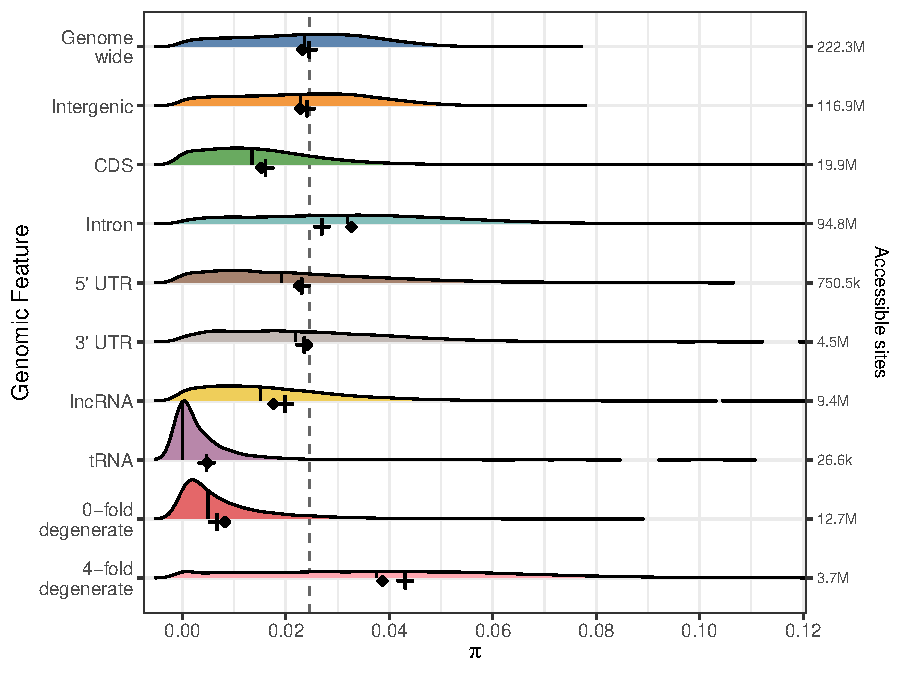
\includegraphics[width=0.6\textwidth]{figures/feature_pi.pdf}
    \caption{\textbf{Nucleotide diversity ($\pi$) across genomic
        features in Oregon \balgla.}
        The density histogram shows the distribution of windowed
        $\pi$ values across different genomic features annotated
        in the \bgla{} assembly. The vertical lines show the
        50\textsuperscript{th} quantile (median) of the distribution,
        while the crosses show the mean value.}
    \label{fig:feature_pi}
\end{figure}

\subsection*{Linkage disequilibrium decays within a few hundred base pairs}\label{sec:results_ld}

\llabel{ld_decay_results}To describe recombination along the genome, we measured how linkage
disequilibrium (LD) decays with the distance between SNPs.
With only six unphased diploid individuals, the usual measures of LD are not reliable.
In 10\,kbp windows, the mean $r^{2}$ between SNPs \citep[$Z_{nS}$;][]{kelly_test_1997},
calculated from genotypes \citep{rogers_linkage_2009}, was close to its sampling floor
for six individuals (median: 0.247), and it decreased as the number of SNPs in the
window increased (Spearman's $\rho$: $-0.52$).
Thus, windows with different SNP densities could not be compared.
We therefore used \sdsq{}, the ratio of the expected $D^{2}$ to the expected
product of allele-frequency variances at the two sites ($\pi_{2}$)
\citep{ohta_linkage_1969}.
We calculated $D^{2}$ and $\pi_{2}$ with the estimators of
\citet{ragsdale_unbiased_2020}, which are unbiased for the size of the sample and
use genotypes, so they do not need phased haplotypes.
Because these estimators are summed over all pairs of SNPs in a distance class,
\sdsq{} does not depend on the number of SNPs, and it can be compared among
regions with different levels of diversity
(see \nameref{sec:methods_ld}).
\vspace{0.1cm}

LD in \bgla{} decays over a short physical distance.
Over the 93 segments of chromosomes 1--15 (see below), \sdsq{} fell to half
of its value for SNPs 10--20\,bp apart at 162\,bp (95\% CI: 142--185\,bp), and to one
quarter at 705\,bp (579--880\,bp; Figure~\ref{fig:sup_ld_decay}A).
A fit of the equilibrium expectation of \citet{ohta_linkage_1971} gave a population
recombination rate ($4N_{e}r$) of 0.14 (0.12--0.17) per bp.
Divided by the median segment $\pi$ (0.024), this value gives $r/\mu \approx 6$.
However, the equilibrium model does not fit the shape of the decay well: the observed
\sdsq{} is 0.7 times the expected value at 14\,bp, and it is 15 times the
expected value at 10\,kbp (Figure~\ref{fig:sup_ld_decay}A).
We therefore use the fitted $4N_{e}r$ as a summary of the rate of decay, not as an
exact estimate of the recombination rate.
\vspace{0.1cm}

The genome contains large regions of reduced diversity (Figure~\ref{fig:genome_pi}D).
To compare them with the rest of the genome, we divided chromosomes 1--15
(excluding chromosome 16 due to its smaller size and uniformly low $\pi$)
into segments of constant mean $\pi$ with a changepoint method
(see \nameref{sec:methods_segments}).
Of the 93 segments, 29 had $\pi$ lower than 0.75 times the genome-wide value
(low-diversity segments; 199\,Mbp, median length 7.1\,Mbp), and 64 did not
(normal-diversity segments; 632\,Mbp, median length 8.9\,Mbp).
The median $\pi$ was 0.0132 in low-diversity segments and 0.0286 in normal-diversity
segments.
LD was higher in the low-diversity segments at all distances
(Figure~\ref{fig:sup_ld_decay}B).
In these segments, \sdsq{} fell to half of its short-distance value at
373\,bp (316--448\,bp), versus 150\,bp (132--174\,bp) in normal-diversity segments, and the
fitted $4N_{e}r$ was 0.036 per bp (0.028--0.051), against 0.15 per bp (0.13--0.18).
We then asked if a difference in $N_{e}$ alone explains this difference in LD decay.
If the two classes differed only in $N_{e}$, the low-diversity curve would equal the
normal-diversity curve with its distances scaled by the ratio of $\pi$ between the
two classes (0.46).
It did not: at the scaled distances, the low-diversity segments had 1.4 to 2.2 times
more LD, and the 95\% confidence intervals did not include 1 at any distance
(Figure~\ref{fig:sup_ld_decay}C).
The ratio of $4N_{e}r$ to $\pi$, which estimates $r/\mu$, gives the same result.
It was 2.7 (2.2--4.3) in the low-diversity segments, against 5.4 (4.6--6.3) in the
normal-diversity segments (ratio 0.51, 0.38--0.83).
Thus, our low-diversity segments have less recombination per mutation, additional LD
caused by linked selection, or both.

\subsection*{Diversity, but not divergence, increases with the population recombination rate}\label{sec:results_pi_rho}

\llabel{pi_rho_results}Linked selection, either background selection or recurrent
selective sweeps, removes more neutral diversity where recombination is low
\citep{kaplan_hitchhiking_1989,begun_levels_1992,charlesworth_effect_1993}.
To test for this pattern, we fitted $4N_{e}r$ in 1\,Mbp windows inside each segment
(827 windows) and compared it with $\pi$ in the same windows.
Because windows in one segment are not independent, all confidence intervals come
from resampling whole segments.
In the normal-diversity segments, $\pi$ increased with $4N_{e}r$ (Spearman's $\rho$:
0.53, 95\% CI: 0.40--0.63; 631 windows).
The correlation was similar when we included the low-diversity segments
(Spearman's $\rho$: 0.48, 0.33--0.60; 827 windows).
Some windows with very low diversity ($\pi < 0.008$) likely contain a large proportion of
genotyping errors, which carry no LD and increase the fitted $4N_{e}r$.
When we removed these 59 windows, the correlation in all segments was 0.57
(0.46--0.66).
The same pattern was present among whole segments (normal-diversity: 0.66, 0.52--0.81;
normal- and low-diversity: 0.59, 0.41--0.73).
Within the low-diversity segments alone, we found no clear relationship
(Spearman's $\rho$: $-0.26$, $-0.49$--0.03; 196 windows), and the negative value came
from the windows with $\pi < 0.008$.
\vspace{0.1cm}

\llabel{div_rho_results}A positive correlation between diversity and recombination
has two possible causes.
Under linked selection, $N_{e}$ is lower where recombination is low, and this reduces
diversity but not divergence between species.
If recombination is mutagenic, the mutation rate is higher where recombination is
high, and this increases both diversity and divergence
\citep{begun_levels_1992}.
To separate these causes, we compared $4N_{e}r$ with divergence between \bgla{} and
\textit{B. crenatus} at 4-fold degenerate sites ($d_{4}$) in the exons of the same
1\,Mbp windows.
In these windows, $\pi$ at 4-fold degenerate sites ($\pi_{4}$) increased with
$4N_{e}r$ (Spearman's $\rho$: 0.39, 0.27--0.50, in 611 normal-diversity windows; 0.43,
0.30--0.54, in all 790 windows).
However, $d_{4}$ did not increase with $4N_{e}r$ (normal-diversity: $-0.05$,
$-0.21$--0.11; all: $-0.08$, $-0.21$--0.07).
The upper limits of these confidence intervals are much lower than the correlation of
$\pi_{4}$ with $4N_{e}r$, so this result is not due to a lack of statistical power.
Also, $d_{4}$ was not correlated with $\pi$ (normal-diversity: 0.09, $-0.05$--0.24;
all: 0.11, $-0.03$--0.25).
The ratio $\pi_{4}/d_{4}$, which removes differences in the mutation rate among
windows, increased with $4N_{e}r$ at least as much as $\pi_{4}$ did (normal-diversity:
0.44, 0.32--0.55; all: 0.47, 0.32--0.58).
Thus, mutagenic recombination does not explain the correlation between diversity
and recombination in \bgla{}.
\vspace{0.1cm}


% Note, update this. The new panel in the main figure covers this so we
% need to make sure they are in sync.
Both $\pi$ and $4N_{e}r$ are proportional to $N_{e}$.
Thus, their correlation is expected when $N_{e}$ varies along the genome, as it does
under linked selection, even if $r$ is constant.
In normal-diversity windows, the slope of $\log(4N_{e}r)$ on $\log(\pi)$ was 1.46
(0.87--2.08), which includes the value of 1 expected if only $N_{e}$ varies.
Together, these results show that the variation in $\pi$ along the genome is a
variation in $N_{e}$, not in the mutation rate, as expected under linked selection.

Both $\pi$ and $4N_{e}r$ are proportional to $N_{e}$.
Thus, their correlation is expected when $N_{e}$ varies along the genome, even if $r$
is constant; in that case, the slope of $\log(4N_{e}r)$ on $\log(\pi)$ is 1.
Among normal-diversity segments, the slope was 2.53 (1.94--3.12;
Figure~\ref{fig:genome_pi}E), and it was 1.92 (1.34--2.45) among normal-diversity
windows. Both exclude 1, so $4N_{e}r/\pi$, which estimates $r/\mu$, increases with $\pi$.
Because $d_{4}$ did not increase with $4N_{e}r$, this is not caused by variation in the
mutation rate, but by a higher recombination rate where diversity is higher.
The relationship remained when we controlled for the number of SNPs and the length of
each segment (partial Spearman's $\rho$: 0.55, 0.35--0.73), and $\sigma_{D}^{2}$ for
SNPs 20--30\,bp apart, which does not depend on the Ohta--Kimura model, decreased with
$\pi$ under the same control ($-0.57$, $-0.74$ to $-0.37$).
Together, these results show that diversity along the \bgla{} genome is lower where
recombination is lower, as expected under linked selection, and that this pattern is
not explained by variation in the mutation rate.


\subsection*{\balgla{} exhibits large effective population sizes}

We estimated the effective population size (\Ne{}) for a central
Oregon \textit{B. glandula} population sample using the whole-genome genotypes.
As a simple estimate of the long-term \Ne{} of this population, we first
calculated \Ne{} using Watterson's estimator of genetic diversity ($\theta_\text{W}$),
observing a mean genome-wide $\theta_\text{W}$ of 0.0617\comment{[Old pixy value; pixy dropped invariant sites with QUAL $<$ 30, so $\pi$ and $\theta_W$ are about 2$\times$ too high. Corrected pooled $\theta_W$ = 0.0294, which gives $N_e \approx 2.5\times10^{6}$ with $\mu = 3\times10^{-9}$. Update.]} (median: 0.0635, standard
deviation: 0.0224; Figure~\ref{fig:sup_theta_ne}). Assuming a per-base,
per-generation mutation rate ($\mu$) of $3\times10^{-9}$ (as estimated by
\cite{nunez_footprints_2020} for the northern acorn barnacle \textit{S. balanoides})
and using the relationship between \Ne{} and $\theta_\text{W}$, this yields a
mean effective size of 5{,}137{,}172 (median: 5{,}289{,}211, standard deviation:
1{,}862{,}683), which is consistent with the expectation of large \Ne{} in this species.
\vspace{0.1cm}

Additionally, we estimated \Ne{} through time using a coalescent-based
approach with \textsc{msmc2} \citep{dutheil_msmc_2020}. This estimate also placed
the historical effective size of the population on the order of $10^{6}$ individuals
(between $10^{6}$ and $10^{7}$ generations ago) (Figure~\ref{fig:sup_mcmc_ne});
however, given our small sample size and the use of only within sample pairwise
comparisons, we were unable to obtain accurate \Ne{} estimates at more recent
($<10^{5}$ generations) timescales using \textsc{msmc2}.
Nevertheless, even these conservative estimates place \bgla{} among the
largest known effective population sizes for any eukaryote, yet orders of
magnitude below the census sizes observed in the field --- a disparity
central to Lewontin's Paradox and one we return to in the Discussion.

\section*{Discussion}\label{sec:discussion}

\subsection*{Genome evolution in large populations}

Evolutionary processes at large demographic scales are expected to leave distinct
signatures in the genome, several of which are observed in our Pacific acorn
barnacle assembly.
For example, large populations are expected to harbor increased levels of segregating
polymorphism, the product of both the reduction in the stochastic loss due to
genetic drift and the increase in the population-scaled mutation rate.
In accordance, we observe a barnacle genome with extreme levels of genetic diversity,
both at the individual and population level (Figure~\ref{fig:sup_kmers};
Table~\ref{tab:sup_popgen_stats}), a substantial proportion of which is located in
coding sequences.
\vspace{0.1cm}

Similarly, large populations are expected to experience an increase in the efficacy of
purifying selection, which is expected to reduce the levels of diversity and increase 
conservation across functional sequences.
We see these patterns reflected in the \bgla{} genome.
Putatively functional sites, particularly coding exons and tRNAs, show both increased
levels of sequence conservation (Figure~\ref{fig:phastcons}) and a reduction in
population-level genetic diversity (Figure~\ref{fig:feature_pi};
Table~\ref{tab:sup_feature_pi}) compared to less constrained features of the genome.
Notably, the rank ordering of the enrichment of conserved elements, with tRNAs and CDSs
as the most enriched, parallels findings in insects \citep{siepel_evolutionarily_2005},
suggesting that the targets of purifying selection are broadly conserved across
arthropods despite the much larger and more repeat-rich genome of \bgla{}.
Increased efficacy of purifying selection is also reflected in the results of the
McDonald-Kreitman test (Figure~\ref{fig:mkTest}), where we observe a relative decrease
in the proportion of non-synonymous polymorphism in a central Oregon \bgla{} population,
suggesting that weakly deleterious variants are more efficiently purged by selection
\citep{li_reverse_2008}.
Positive selection is also expected to increase in efficacy in large populations,
resulting in the fixation of a larger fraction of beneficial non-synonymous mutations.
We observe this pattern as well: in this central Oregon population, the majority
(54 to 61\%, depending on the metric of $\alpha$ used) of non-synonymous substitutions
reached fixation due to positive selection, a proportion higher than that observed in
diverse \textit{Drosophila} populations \citep{haller_asymptoticmk_2017}.
\vspace{0.1cm}

In large enough populations, selection should be efficacious enough that its effects
extend to synonymous sites, where substitutions are normally considered neutral.
This could result in a bias in the usage of synonymous codons, as different codons are
favored over others due to GC biases, mRNA stability, tRNA abundance, and other factors
\citep{galtier_codon_2018,presnyak_codon_2015}.
These effects are observed in the \bgla{} assembly in the form of reduction in the
effective number of codons seen across protein-coding genes.
On average, \bgla{} uses $\approx$ 43 out of 61 available codons, a greater reduction than
that observed in other metazoan genomes (Figure~\ref{fig:codon_enc};
Table~\ref{tab:sup_enc_summary}).
There is moderate evidence that this bias is not the product of compositional neutral
processes (Figure~\ref{fig:sup_enc_gc3s};~Figure~\ref{fig:sup_enc_reg}), suggesting an
increase in the efficacy of natural selection due to the large size of Pacific acorn
barnacle populations.
Moreover, these biases put into question the neutrality of at least some synonymous
substitutions in this system, which could have important ramifications for the study of
molecular evolution; however, the extent of these effects remain presently unknown and
should be the subject of future study.
\vspace{0.1cm}

In contrast, the distribution of transposable and repeat elements in the
\bgla{} assembly was unexpected, as we find a highly repetitive genome
composed of over 60\% repeats (Figure~\ref{fig:genome_pi};
Table~\ref{tab:sup_repeat_summary}).
Previous work has shown that purifying selection plays a key role in the accumulation
and fixation of transposable elements \citep{merel_relaxed_2025,langmuller_genomic_2023,
bourque_ten_2018}, following the expectation that repetitive sequences are, on average,
slightly deleterious.
Given the increased efficacy of selection we observed in the rest of the genome,
our expectation was to find a relatively small proportion of repeats.
However, the high repeat content observed in the genome does not necessarily
reflect the low efficacy of selection in these populations.
Some could be low-frequency, slightly deleterious variants in the process of being purged
from the population.
Other repeats might represent beneficial genetic variation, as transposable elements are
known to play roles in adaptive evolution \citep{schrader_impact_2019}.
For example, repeat elements can act as regulators of gene expression
\citep{trizzino_transposable_2017,rech_population-scale_2022}, and as such may provide
the regulatory plasticity required for survival in rapidly changing
intertidal environments.
Regardless of their role, disentangling the population-wide repeat landscape and its
fitness effects is likely impossible with a single haploid reference assembly.
Thus, this observation drives the need for larger comparative genomic studies across
barnacle populations before we can fully understand the dynamics of genomic repeats
and transposable elements in this and other large populations.

\subsection*{Molecular evolution in large populations: reconciling \dnds{} and the
McDonald-Kreitman test}\label{sec:discussion_dnds_mkt}

One of the more striking patterns in our results is the apparent discordance between
our two measures of selection on protein-coding genes.
The average pairwise \dnds{} between \bgla{} and \textit{B. crenatus} is 0.206,
indicating that the majority of coding sites are under purifying selection.
Yet the McDonald-Kreitman test reveals a seemingly opposite pattern: $\approx61\%$
of non-synonymous substitutions fixed between these species were driven by
positive selection ($\alpha_\text{asym}$ = 0.610).
At first glance, these results appear contradictory: how can coding sequences be
under strong purifying selection while simultaneously showing pervasive adaptive
evolution?
\vspace{0.1cm}

The resolution lies in the fact that \dnds{} and the McDonald-Kreitman test measure
fundamentally different quantities. The \dnds{} ratio averages across all
non-synonymous sites in a gene, the vast majority of which are under functional
constraint, resulting in a ratio well below one. In contrast, the McDonald-Kreitman
test partitions changes into polymorphism and divergence, using synonymous changes
as a neutral baseline to ask whether there is an \textit{excess} of non-synonymous
fixations relative to the neutral expectation. This test is therefore sensitive to
the subset of non-synonymous mutations that escape purifying selection and reach
fixation, even when most non-synonymous sites in a gene are constrained.
Moreover, pairwise \dnds{} is calculated from a single sequence per species and
therefore incorporates segregating polymorphisms into its divergence estimate. In
species with many weakly deleterious non-synonymous variants segregating at
appreciable frequencies, this can inflate the non-synonymous divergence and distort
estimates of selection \citep{li_reverse_2008}. By explicitly separating
polymorphism from fixation, the McDonald-Kreitman test avoids this conflation.
\vspace{0.1cm}

\citet{li_reverse_2008} compared the performance of \dnds{} and the McDonald-Kreitman
test across human, \textit{Drosophila}, and yeast genomes and found that the two
approaches identify distinct but correlated sets of genes as targets of selection.
Notably, the McDonald-Kreitman test was more powerful than \dnds{} only in
\textit{Drosophila}, the species with the highest polymorphism, where it
identified nearly three times as many genes under positive selection. In the
lower-diversity human and yeast datasets, the pattern was reversed. This finding
suggests that the statistical power of the McDonald-Kreitman test is greatest in
high-polymorphism species, making it particularly well suited for systems like
barnacles where segregating variation is abundant.
\vspace{0.1cm}

The pattern we observe in \bgla{} is thus consistent with theoretical expectations
for large populations: strong purifying selection efficiently removes the majority
of deleterious non-synonymous mutations, keeping \dnds{} low, while at the same time
the increased efficacy of positive selection drives a disproportionate fraction of
the remaining non-synonymous substitutions to fixation, producing a high
$\alpha$. This coupling of strong purifying and positive selection is a hallmark
of evolution in large populations and has been observed in \textit{Drosophila}, where
$\alpha_\text{asym}$ is approximately 0.57 \citep{messer_frequent_2013}.
Our estimate of $\alpha_\text{asym}$ of 0.610 in \bgla{} is comparable to
or slightly higher than that in \textit{Drosophila}, consistent with the expectation
that the even larger effective population size in barnacles further increases the
efficacy of both modes of selection.
\vspace{0.1cm}

\subsection*{Barnacles as models for evolution at biological extremes}

Our work shows that a Pacific acorn barnacle population from central Oregon exhibits
genetic diversity of over 5\% (mean genome-wide $\pi$ of 0.0506).\comment{[Old pixy value; pixy dropped invariant sites with QUAL $<$ 30, so $\pi$ and $\theta_W$ are about 2$\times$ too high. Corrected genome-wide $\pi$ = 0.023 (\texttt{pg\_gpu\_stats}). Update.]}
These levels of genetic diversity are higher than those observed for other model
systems known for their relatively large population sizes.
For example, the genome-wide $\pi$ we observe in this population is approximately
seven-fold\comment{[Old pixy value; pixy dropped invariant sites with QUAL $<$ 30, so $\pi$ and $\theta_W$ are about 2$\times$ too high. With the corrected $\pi$ this ratio is about 3-fold. Update.]} higher than that observed in sub-Saharan populations of
\textit{D. melanogaster} (Figure~\ref{fig:sup_pi_comp})
\citep{nunez_footprints_2025,li_comparative_2025,pool_population_2012,
langley_genomic_2012}.
Indeed, even the $\pi$ observed at 0-fold degenerate sites, the least diverse and
among the most constrained sites in the genome, exceeds the genome-wide diversity
observed in these \textit{Drosophila} populations.\comment{[Old pixy value; pixy dropped invariant sites with QUAL $<$ 30, so $\pi$ and $\theta_W$ are about 2$\times$ too high. The corrected 0-fold $\pi$ (0.0067) no longer exceeds the \textit{Drosophila} genome-wide mean (0.0076, Figure~\ref{fig:sup_pi_comp}); remove or reword this sentence. Update.]}
While elevated, this level of diversity is not unique to barnacles.
Similar magnitudes of genome-wide $\pi$ ($\approx10^{-2}$) have been observed
in other metazoan taxa, including corals \citep{meziere_corals_2025}, bivalves
\citep{liu_bivalves_2025}, mosquitoes \citep{kent_aedes_2025,ag1000g}, nematodes
\citep{teterina_nematodes_2023}, and lancelets \citep{braso-vives_highly_2026}.
The bivalve values, however, were computed from variant sites only, after the removal
of sites with a minor allele frequency below 5\% \citep{liu_bivalves_2025}; they are
therefore not per-site diversities and are not directly comparable to ours.
Moreover, as with other marine invertebrates, barnacle life history traits are likely
direct drivers of the elevated polymorphism observed, as factors such as large census
sizes, small propagule size, large brood size, long larval dispersal, and broad geographic
distribution have been positively correlated with high genetic diversity in these
organisms \citep{leffler_revisiting_2012,romiguier_comparative_2014}.
\vspace{0.1cm}

The magnitude of diversity observed in \bgla{} solidly places them among
hyperpolymorphic populations, those exhibiting diversity above 5\%\comment{[Old pixy value; pixy dropped invariant sites with QUAL $<$ 30, so $\pi$ and $\theta_W$ are about 2$\times$ too high. With corrected values, 4-fold $\pi$ = 4.2\% and genome-wide $\pi$ = 2.3\%; reword. Update.]}
\citep{cutter_molecular_2013}. This adds barnacles to a growing list of emerging
hyperpolymorphic model systems, which are key to studying the limits of biological
variation and molecular evolution in natural populations. Moreover, our observations
of extreme genetic diversity also have important implications for the study of species
boundaries. For example, recent work by~\citet{hart_genomic_2025} suggests that levels
of polymorphism above 1\% neutral diversity in eukaryotes likely serve as biological limits
for the definition of species. Barnacles and other hyperpolymorphic populations put these
putative cutoffs into question. We observe levels of genome-wide diversity of over 5\%
in just a very small portion of the biological range of the Pacific acorn barnacle.
Nucleotide diversity is even higher ($\approx8\%$\comment{[Old pixy value; pixy dropped invariant sites with QUAL $<$ 30, so $\pi$ and $\theta_W$ are about 2$\times$ too high. Corrected 4-fold $\pi$ = 4.2\%. Update.]}) at 4-fold degenerate, and putatively
neutral, sites (Figure~\ref{fig:feature_pi}; Table~\ref{tab:sup_feature_pi}).
Given the species' broader geographical and ecological distribution, genetic
diversity is likely to increase when looking across a larger spatial sampling.
This observation reiterates the importance of future studies of genetic diversity
of this species over its whole geographic range, providing some insights on
the mechanisms that maintain population and species boundaries in the presence
of extreme genetic diversity.
\vspace{0.1cm}

Beyond species boundaries, the extreme diversity observed in barnacles also speaks to
a long-standing question in population genetics: the relationship between effective
and census population sizes. From our results on diversity, we
observe that this barnacle population has an effective size of approximately $10^{6}$.\comment{[Old pixy value; pixy dropped invariant sites with QUAL $<$ 30, so $\pi$ and $\theta_W$ are about 2$\times$ too high. Recompute with the corrected $\theta_W$; see also the sea star rate below. Update.]}
However, these populations also show densities of $10^{4}$ individuals per square meter
\citep{menge_recruitment_2000}. Based on this estimate, the census size of the Pacific
acorn barnacle population in central Oregon should be, conservatively, in the billions of
individuals. While the general disparity between the effective and census size estimates
has been highlighted for decades, i.e., Lewontin's Paradox \citep{lewontin_genetic_1974},
the mechanisms underlying the differences have been long debated
\citep{gillespie_role_1999,gillespie_genetic_2000,smith_hitch-hiking_1974,
kimura_neutral_1983} and are still the subjects of study \citep{buffalo_quantifying_2021}.
Our work on the Pacific acorn barnacle provides a unique opportunity to empirically
study this disparity and the biological processes that maintain it.
\vspace{0.1cm}

\subsection*{Barnacles among highly fecund marine invertebrates}

\llabel{marine_sweepstakes}\revpoint{2}{5}With census sizes in the billions and high fecundity,
\bgla{} belongs to the group of marine invertebrates in which the relationship between
census size, effective size, and diversity has been debated for decades.
High fecundity combined with high early mortality can produce a very large variance in
reproductive success, such that a small fraction of adults produces most of the recruits
in each generation.
This sweepstakes reproductive success predicts ratios of effective to census size far
below one and genetic differences among cohorts and sites at small spatial scales
(chaotic genetic patchiness) \citep{hedgecock_does_1994}, and, when the variance is
extreme, genealogies with multiple mergers rather than the Kingman coalescent
\citep{eldon_coalescent_2006}.
Multiple-merger genealogies give an excess of rare variants and can bias estimates of
effective size and demographic history made under the Kingman coalescent.
The negative genome-wide Tajima's $D$ we observe is consistent with population growth,
with linked selection, and with sweepstakes reproduction, and our sample of six
individuals cannot separate these processes.
Our estimates of \Ne{} should therefore be read as the effective size of an equivalent
Kingman population.
\vspace{0.1cm}

\llabel{marine_oysters}Bivalves provide the closest precedent for the patterns in coding sequences that we
report.
In the Pacific oyster, \citet{sauvage_single_2007} found among the highest densities of
synonymous polymorphism then known in animals and studied their relation to codon
usage.
In the European flat oyster, \citet{harrang_high_2013} found a high load of non-neutral
amino-acid polymorphisms: the ratio of non-synonymous to silent diversity was 0.38, at
a synonymous diversity of only 0.006, and the authors related this load to sweepstakes
reproduction.
\bgla{} does not follow this pattern.
Its synonymous diversity is about seven times higher ($\pi_S = 0.042$) and its
$\pi_N/\pi_S$ is about one third as high (0.11).\comment{[Corrected values, from the MK
alignments with all invariant sites counted (revision\_analysis
\texttt{results/comparative}); they replace the pixy values used elsewhere in the
manuscript.]}
This value is inside the range predicted from the synonymous diversity of 86 animal
species, and inside the range of the marine invertebrates among them
\citep{romiguier_comparative_2014,galtier_adaptive_2016}
(Figure~\ref{fig:sup_comparative}).
A high load of amino-acid polymorphism is thus not a general property of highly fecund
marine invertebrates, and in \bgla{} purifying selection on amino-acid variation is as
efficient as its synonymous diversity predicts.
\vspace{0.1cm}

\llabel{marine_sv}Marine invertebrate genomes also carry extensive structural variation.
Gene presence-absence variation is widespread in the Mediterranean mussel
\citep{gerdol_massive_2020}; duplications cover 16.5\% of the eastern oyster genome
across 60 individuals \citep{modak_extensive_2021}; sequences present in only one
haplotype make up about 69\% of each haplotype of a \textit{Crassostrea sikamea}
genome \citep{liu_bivalves_2025}; inversion polymorphisms segregate in \textit{Ciona}
\citep{satou_chromosomal_2021}; and copy number variants make up about one fifth of
sequenced loci in the American lobster, where they, and not SNPs, are associated with
sea temperature \citep{dorant_copy_2020}.
The \bgla{} genome shows signs of the same complexity: a $k$-mer heterozygosity above
3\% (Figure~\ref{fig:sup_kmers}), about 240\,Mbp of haplotig sequence removed during
assembly (Table~\ref{tab:sup_asm_stats}), and a repeat content above 60\%.
Our SNP-based analyses do not capture this variation.
Population samples sequenced with long reads will be necessary to measure the total
genetic variation in \bgla{} and to test whether, as in the lobster, structural
variants carry a large part of its adaptive variation.
\vspace{0.1cm}

\llabel{marine_mutation_rate}Direct estimates of the germline mutation rate now exist for highly
fecund marine invertebrates.
In the crown-of-thorns sea star, $\mu = 9.13 \times 10^{-9}$ per site per generation
(95\% CI $6.5 \times 10^{-9}$ to $1.2 \times 10^{-8}$), from 14 parent-offspring trios
\citep{popovic_high_2024}, three times the rate we used here.
With this rate, our genome-wide diversity gives a long-term \Ne{} of about
$6 \times 10^{5}$ (about $1.2 \times 10^{6}$ from 4-fold degenerate sites), which makes
the gap to census size even larger.\comment{[From corrected $\pi$: genome-wide 0.0231,
4-fold 0.0423.]}
In tunicates, the estimates are indirect, and they suggest a per-generation rate no
higher than in vertebrates \citep{tsagkogeorga_population_2012}.
A high mutation rate thus does not appear to explain the high diversity of these
species, and the gap between effective and census size must come from other processes,
such as linked selection or sweepstakes reproduction.

\section*{Conclusion}

In this work, we take one of the first looks at the genomic signatures of evolution
in large populations using the Pacific acorn barnacle, \balgla{}.
In accordance with population genetics theory, we find evidence for the increased
efficacy of selection in this large barnacle population, manifested as both purifying
selection reducing diversity and maintaining conservation across functional sites, and
pervasive positive selection driving adaptive divergence in protein-coding genes.
Surprisingly, however, we find a highly repetitive genome, in apparent contrast to
the expectation that purifying selection should limit the proliferation of repetitive
sequences.
At the population scale, we observe average genome-wide
nucleotide diversity exceeding 5\%\comment{[Old pixy value; pixy dropped invariant sites with QUAL $<$ 30, so $\pi$ and $\theta_W$ are about 2$\times$ too high. Corrected genome-wide $\pi$ = 0.023 (\texttt{pg\_gpu\_stats}). Update.]}, placing this species among hyperpolymorphic
organisms.
Yet, while this diversity implies large effective population sizes ($\approx10^{6}$\comment{[Old pixy value; pixy dropped invariant sites with QUAL $<$ 30, so $\pi$ and $\theta_W$ are about 2$\times$ too high. Recompute $N_e$ from the corrected $\theta_W$ (0.028). Update.]}
individuals), it still pales in comparison to the estimated census sizes
of this population, underscoring the long-standing disparity between effective
and census population sizes.
Together, these findings establish \bgla{} as a promising emerging model for studying
the mechanisms of evolution at biological extremes.


\input{sections/data_avail.tex}
\input{sections/acknowledgments}
\input{sections/author_contributions}

% Clear a new page for the bibliography
\clearpage

\printbibliography

% Supplements
\clearpage

\fancyhead[L]{\textit{SUPPLEMENTS}}

\input{sections/supplement_methods}

\clearpage

\section*{Supplemental Tables}

% Stats for the different stages of the assembly
\begin{table}[ht]
    \centering
    \suptablecaption{\textbf{Assembly statistics for the \balgla{} genome
        at different stages of the assembly process.}
        Default contigs refers to the sequences assembled by \textsc{hifiasm} with
            default parameters.
        Optimized contigs denotes the sequences generated using \textsc{hifiasm}
            followed by removal of contaminant sequences and purging of haplotigs.
        Hi-C scaffolds refer to the scaffolds generated by \textsc{YaHS}.
        Curated assembly refers to the sequences generated after manual curation of 
            the Hi-C contact map and polishing with \textsc{Inspector}.
        \textsc{BUSCO} results refer to the \texttt{arthropoda\_odb10} dataset.}
    \shadedrows
    \begin{tabular}{lrrrr}
        \toprule
        Assembly Stage &
            \shortstack{Default \\ contigs} &
            \shortstack{Optimized \\ contigs} &
            \shortstack{Hi-C \\ scaffolds} &
            \shortstack{Curated \\ assembly} \\
        \midrule \startshading
        Sequence length (Mbp)          & 1.64        & 1.05        & 1.05       & 1.04 \\
        Fragments (N)                  & \num{4212}  & \num{1342}  & 650        & 592 \\
        Contig N50 (Mbp)               & 0.734       & 1.35        & 1.18       & 1.18 \\
        Scaffold N50 (Mbp)             & \texttt{NA} & \texttt{NA} & 50.96      & 51.41 \\
        \textsc{BUSCO} complete (\%).  & 95.66       & 93.88       & 93.98      & 94.08 \\
        \textsc{BUSCO} single (\%)     & 45.31       & 89.04       & 89.24      & 89.44 \\
        \textsc{BUSCO} duplicates (\%) & 50.35       & 4.84        & 4.74       & 4.64 \\
        \textsc{BUSCO} fragmented (\%) & 0.79        & 1.18        & 0.89       & 0.89 \\
        \textsc{BUSCO} missing (\%)    & 3.55        & 4.94        & 5.13       & 5.03 \\
        \textsc{BUSCO} size (N)        & \num{1013}  & \num{1013}  & \num{1013} & \num{1013} \\
        \bottomrule
    \end{tabular}
    \label{tab:sup_asm_stats}
\end{table}

% Gene-completeness in the annotation
\begin{table}[ht]
    \centering
    \suptablecaption{\textbf{Completeness metrics for the \balgla{} protein-coding
        gene annotation.}
        \textsc{BUSCO} completeness was determined by \textsc{compleasm}
        \texttt{protein}.}
    \shadedrows
    \begin{tabular}{lrr}
        \toprule
        Metric &
            \texttt{arthropoda\_odb10} &
            \texttt{crustacea\_odb12} \\
        \midrule \startshading
        \textsc{BUSCO} complete (\%)   & 93.58      & 84.77 \\
        \textsc{BUSCO} single (\%)     & 79.76      & 72.66 \\
        \textsc{BUSCO} duplicates (\%) & 13.82      & 12.11 \\
        \textsc{BUSCO} fragmented (\%) & 1.78       & 4.10 \\
        \textsc{BUSCO} missing (\%)    & 4.64       & 11.13 \\
        \textsc{BUSCO} size (N)        & \num{1013} & \num{1536} \\
        \bottomrule
    \end{tabular}
    \label{tab:sup_annot_stats}
\end{table}

% Repeat annotation
\begin{table}[htbp]
\centering
\suptablecaption{\textbf{High-level repeat annotation of the \balgla{}
        assembly.}
            Repeats were first identified with the \textsc{EarlGrey} software.
            The classification is the merge of \textsc{EarlGrey}'s homology-based
            assignment, followed by the re-classification of unknown elements by
            \textsc{TEsorter} and \textsc{DeepTE}.
            Coverage is the total number of masked sites per class; ``\% Genome''
            is the coverage divided by assembly size (1{,}043{,}519{,}078\,bp).}
    \label{tab:sup_repeat_summary}
    \shadedrows
    \begin{tabular}{lrrrr}
        \toprule
            Classification &
                Coverage (bp) &
                Count &
                \% Genome &
                \shortstack{Distinct \\ elements} \\
        \midrule \startshading
            DNA                                        & \num{379178613} & \num{895512}  & 36.34 & 35 \\
            LINE                                       & \num{107103442} & \num{223314}  & 10.26 & 20 \\
            LTR                                        & \num{50161694}  & \num{120887}  &  4.81 &  8 \\
            \shortstack[l]{Other (Simple Repeat, \\
                ~~Microsatellite, RNA)}                & \num{37359678}  & \num{74786}   &  3.58 &  3 \\
            Penelope                                   & \num{25833119}  & \num{65921}   &  2.48 &  4 \\
            Rolling Circle                             & \num{22238826}  & \num{42257}   &  2.13 &  1 \\
            Retroposon                                 & \num{2095328}   & \num{5834}    &  0.20 &  2 \\
            SINE                                       & \num{1253619}   & \num{4437}    &  0.12 &  3 \\
            DIRS                                       & \num{1184091}   & \num{1285}    &  0.11 &  2 \\
            Unclassified                               & \num{61450725}  & \num{148647}  &  5.89 &  1 \\
            \midrule
            Total                                      & \num{687859135} & \num{1582880} & 65.92 & 79 \\
    \bottomrule
    \end{tabular}
\end{table}

% Stats about polymorphism in the reference individual and the popgen samples.
\begin{table}[ht]
    \centering
    \suptablecaption{\textbf{Genetic variation in central Oregon \balgla{}.}
        \comment{the ref indidivual stats have to be updated}
        Density of SNPs per accessible kbp is calculated only for windows with more
        than 100 accessible sites ($1000 \times N_\text{window SNPs} / N_\text{window accessible}$).
        Density of SNP in coding sequences was calculated only for exons with more than
        100 accessible sites and adjusting for exon length
        ($1000 \times N_\text{exon SNPs} / N_\text{exon accessible}$).}
    \shadedrows
    \begin{tabular}{lrr}
        \toprule
        Metric &
            Reference Individual &
            Cape Perpetua (N=6) \\
        \midrule \startshading
        Reference sequence length (bp)        & \num{904940360} & \num{904940360} \\
        Accessible sites post-filtering (bp)  & \num{314105136} & \num{231589201} \\
        Total variant sites (N)               & \num{9081889}   & \num{21395217} \\
        Percent variant sites (\%)            & 2.89            & 9.24 \\
        SNPs (N)                              & \num{8725877}   & \num{20495291} \\ % 8.85 of sites
        Indels (N)                            & \num{356012}    & \num{899926} \\
        Multiallelic SNPs (N)                 & \texttt{NA}     & \num{910949} \\ % 4.6% of var sites
        Percent multiallelic SNPs (\%)        & \texttt{NA}     & 4.6 \\
        \midrule
            \rowcolor{white}SNP density \\
        \midrule
        % This is 1000 x N_snps / N_accessible in 1000 bp windows
        Mean SNPs per accessible kbp          & 14.66           & 83.3 \\
        Median SNPs per accessible kbp        & 6               & 80.7 \\
        StDev SNPs per accessible kbp         & 19.86           & 53.9 \\
        \midrule
            \rowcolor{white}Coding variation \\
        \midrule
        % This is 1000 x N_exon_snps x N_exon_accessible across each exon interval
        SNPs in CDS (N)                       & \num{398773}    & \num{1061714} \\
        Percent SNPs in CDS (\%)              & 4.69            & 5.18 \\
        Mean SNPs per accessible CDS kbp      & 4.34            & 51.0 \\
        Median SNPs per accessible CDS kbp    & 1               & 46.5 \\
        StDev SNPs per accessible CDS kbp     & 11.75           & 33.8 \\
        \bottomrule
    \end{tabular}
\label{tab:sup_popgen_stats}
\end{table}

% Stats about the phasCons conserved elements and enrichment of genomic elements.
\begin{sidewaystable}[ht]
    \suptablecaption{\textbf{Enchrichment of annotated features among \textsc{phastCons}
        highly conserved elements.}
        The total feature proportion was determined according to the 841{,}166{,}098\,bp
        corresponding to the 16 chromosome-level scaffolds.
        Proportion of highly-conserved elements (HCE) was calculated based on the
        50{,}849{,}898\,bp-span of all HCEs in the genome.
        The number of chromosomes denotes the number of chromosome-level scaffolds
        containing annotations of the given feature.}
    \centering
    \label{tab:sup_phastcons_enrichment}
    \shadedrows
    \begin{tabular}{lrrrrrrrr}
    \toprule
        Feature &
            \shortstack{Total feature \\ length (bp)} &
            \shortstack{Total feature \\ proportion} &
            \shortstack{HCE feature \\ length (bp)} &
            \shortstack{HCE feature \\ proportion} &
            \shortstack{Mean $\log_2$ \\ enrichment} &
            \shortstack{Median $\log_2$ \\ enrichment} &
            \shortstack{St Dev $\log_2$ \\ enrichment} &
            \shortstack{Number of \\ chromosomes} \\
    \midrule \startshading
        3' UTR     & \num{2358104}   & $2.80\mathrm{e}{-3}$ & \num{152598}   & $3.00\mathrm{e}{-3}$ & $-0.0861$    & 0.0332       & 0.508        & 16 \\
        5' UTR     & \num{530151}    & $6.30\mathrm{e}{-4}$ & \num{27679}    & $5.44\mathrm{e}{-4}$ & $-0.292$     & $-0.332$     & 0.453        & 16 \\
        CDS        & \num{16273411}  & 0.0193               & \num{2225138}  & 0.0438               & 0.752        & 0.984        & 0.926        & 16 \\
        TE         & \num{370573528} & 0.441                & \num{17505920} & 0.344                & $-0.359$     & $-0.305$     & 0.180        & 16 \\
        intergenic & \num{196612776} & 0.234                & \num{10688761} & 0.210                & $-0.167$     & $-0.178$     & 0.167        & 16 \\
        intron     & \num{111562654} & 0.133                & \num{8575960}  & 0.169                & 0.419        & 0.297        & 0.432        & 16 \\
        lncRNA     & \num{2211027}   & $2.63\mathrm{e}{-3}$ & \num{130744}   & $2.57\mathrm{e}{-3}$ & $-0.174$     & $-0.133$     & 0.567        & 16 \\
        multiple   & \num{141022121} & 0.168                & \num{11537936} & 0.227                & 0.418        & 0.438        & 0.167        & 16 \\
        rRNA       & \num{2106}      & $2.50\mathrm{e}{-6}$ & 0.000          & 0.000                & \texttt{NaN} & \texttt{NaN} & \texttt{NaN} & 6 \\
        tRNA       & \num{20220}     & $2.40\mathrm{e}{-5}$ & \num{5162}     & $1.02\mathrm{e}{-4}$ & 2.143        & 2.041        & 0.959        & 16 \\
   \bottomrule
\end{tabular}
\end{sidewaystable}

% Breakdown of per-species codon usage bias
\begin{sidewaystable}[ht]
    \centering
    \small
    \suptablecaption{\textbf{Codon usage biases across metazoan genomes.}
        Table shows the codon usage statistics (effective number of codons; ENC), GC
        proportion, and GC proportion at third codon positions (GC3s) for length-filtered
        (CDS $\geq$ 300\,bp, within 2 standard deviations of the per-species mean length)
        genes in each genome.
        The first four rows (\texttt{BalGla}, \texttt{BalCre}, \texttt{AmpAmp}, and
        \texttt{PolPol}) denote the focal barnacle genomes.}
    \label{tab:sup_enc_summary}
    \shadedrows
    \begin{tabular}{llrrrrrrrrrr}
    \toprule
    & & & \multicolumn{3}{c}{ENC} & \multicolumn{3}{c}{GC} & \multicolumn{3}{c}{GC3s} \\
    \cmidrule(lr){4-6} \cmidrule(lr){7-9} \cmidrule(lr){10-12}
    Genome &
        Species &
        \shortstack{Number \\ of Genes} &
        Mean & Median & StDev &
        Mean & Median & StDev &
        Mean & Median & StDev \\
    \midrule \startshading
    \texttt{BalGla} & \balgla{}                              & \num{16217} & 43.17 & 42.84 & 5.52 & 0.645 & 0.648 & 0.061 & 0.781 & 0.796 & 0.102 \\
    \texttt{BalCre} & \textit{Balanus crenatus}              & \num{7675}  & 42.23 & 41.40 & 4.78 & 0.645 & 0.649 & 0.055 & 0.815 & 0.837 & 0.093 \\
    \texttt{AmpAmp} & \textit{Amphibalanus amphitrite}       & \num{25242} & 44.33 & 43.93 & 5.05 & 0.632 & 0.636 & 0.054 & 0.775 & 0.792 & 0.099 \\
    \texttt{PolPol} & \textit{Pollicipes pollicipes}         & \num{17607} & 42.04 & 41.57 & 4.56 & 0.644 & 0.648 & 0.049 & 0.829 & 0.845 & 0.082 \\
    \texttt{DroMel} & \textit{Drosophila melanogaster}       & \num{12312} & 49.97 & 50.47 & 3.99 & 0.534 & 0.540 & 0.053 & 0.630 & 0.640 & 0.110 \\
    \texttt{AnoGam} & \textit{Anopheles gambiae}             & \num{11804} & 48.43 & 48.92 & 5.09 & 0.556 & 0.566 & 0.062 & 0.667 & 0.688 & 0.136 \\
    \texttt{CaeBre} & \textit{Caenorhabditis brenneri}       & \num{22904} & 50.95 & 51.55 & 3.21 & 0.436 & 0.430 & 0.045 & 0.411 & 0.399 & 0.088 \\
    \texttt{MagGig} & \textit{Magallana gigas}               & \num{24963} & 53.34 & 53.66 & 2.58 & 0.442 & 0.441 & 0.043 & 0.433 & 0.426 & 0.085 \\
    \texttt{StrPur} & \textit{Strongylocentrotus purpuratus} & \num{25759} & 53.92 & 54.39 & 2.68 & 0.481 & 0.480 & 0.035 & 0.489 & 0.486 & 0.079 \\
    \texttt{BraLan} & \textit{Branchiostoma lanceolatum}     & \num{23301} & 51.20 & 51.78 & 3.57 & 0.537 & 0.536 & 0.043 & 0.620 & 0.619 & 0.095 \\
    \texttt{CioInt} & \textit{Ciona intestinalis}            & \num{14370} & 52.49 & 52.75 & 2.66 & 0.424 & 0.422 & 0.037 & 0.369 & 0.367 & 0.069 \\
    \texttt{HomSap} & \textit{Homo sapiens}                  & \num{21573} & 49.39 & 50.57 & 4.51 & 0.538 & 0.541 & 0.087 & 0.593 & 0.603 & 0.163 \\
    \bottomrule
    \end{tabular}
\end{sidewaystable}

% Summary of ENC models
\begin{table}[htbp]
    \centering
    \small
    \suptablecaption{\textbf{Summary of ENC model fits across metazoan genomes.}
        Table shows the fits for the model between the expected and observed effective
        number of codons (ENC) across 12 metazoan genomes.
        ENC deviation values represents the deviation from Wright's curve, as shown in
        Figure~\ref{fig:sup_enc_gc3s}.
        Larger ($\gg0$) values denote a reduction in the observed number of effective
        codons when compared to the GC3s-based expectation, suggesting translational
        selection.
        The linear regression values represent the linear relationship between the
        observed and expected number of effective codons, as seen in Figure~\ref{fig:sup_enc_reg}.
        Deviations in ENC product of translational selection are seen as a reduction in
        both slope and coefficient of determination ($\text{R}^2$).
        }
    \label{tab:sup_enc_models}
    \shadedrows
    \begin{tabular}{llrcccccccc}
    \toprule
    & & & \multicolumn{5}{c}{ENC deviation} & \multicolumn{3}{c}{Linear regression} \\
    \cmidrule(lr){4-8} \cmidrule(lr){9-11}
    Genome &
        Species &
        \shortstack{Number \\ of Genes} &
        Mean & Median & StDev & Min & Max &
        Slope & Intercept & $\text{R}^2$ \\
    \midrule \startshading
    \texttt{BalGla} & \bgla{}                  & \num{16217} & 0.065 & 0.053 & 0.090 & $-0.344$ & 0.571 & 0.580 & 16.18 & 0.492 \\
    \texttt{BalCre} & \textit{B. crenatus}     & \num{7675}  & 0.040 & 0.044 & 0.052 & $-0.235$ & 0.382 & 0.725 & 10.19 & 0.844 \\
    \texttt{AmpAmp} & \textit{A. amphitrite}   & \num{25242} & 0.052 & 0.055 & 0.047 & $-0.225$ & 0.517 & 0.747 & 9.27  & 0.868 \\
    \texttt{PolPol} & \textit{P. pollicipes}   & \num{17607} & 0.025 & 0.032 & 0.054 & $-0.265$ & 0.436 & 0.746 & 9.77  & 0.806 \\
    \texttt{DroMel} & \textit{D. melanogaster} & \num{12312} & 0.092 & 0.092 & 0.039 & $-0.125$ & 0.356 & 0.754 & 8.44  & 0.760 \\
    \texttt{AnoGam} & \textit{A. gambiae}      & \num{11804} & 0.074 & 0.075 & 0.040 & $-0.184$ & 0.480 & 0.779 & 7.58  & 0.871 \\
    \texttt{CaeBre} & \textit{C. brenneri}     & \num{22904} & 0.107 & 0.100 & 0.057 & $-0.079$ & 0.518 & 0.436 & 26.00 & 0.175 \\
    \texttt{MagGig} & \textit{M. gigas}        & \num{24963} & 0.079 & 0.076 & 0.040 & $-0.108$ & 0.567 & 0.560 & 20.89 & 0.330 \\
    \texttt{StrPur} & \textit{S. purpuratus}   & \num{25759} & 0.088 & 0.083 & 0.037 & $-0.287$ & 0.465 & 0.853 & 3.51  & 0.358 \\
    \texttt{BraLan} & \textit{B. lanceolatum}  & \num{23301} & 0.085 & 0.082 & 0.046 & $-0.166$ & 0.487 & 0.642 & 15.17 & 0.624 \\
    \texttt{CioInt} & \textit{C. intestinalis} & \num{14370} & 0.060 & 0.057 & 0.038 & $-0.156$ & 0.428 & 0.591 & 19.45 & 0.588 \\
    \texttt{HomSap} & \textit{H. sapiens}      & \num{21573} & 0.086 & 0.091 & 0.046 & $-0.201$ & 0.486 & 0.693 & 11.83 & 0.818 \\
    \bottomrule
    \end{tabular}
\end{table}


% Breakdown of the per-feature Pi
\begin{sidewaystable}[ht]
    \centering
    \small
    \setlength{\tabcolsep}{4pt}
    \suptablecaption{\textbf{Nucleotide diversity ($\pi$) across different genomic features.}
        For all features, pooled $\pi$ denotes the total sum of pairwise differences over
        the sum pairwise comparisons ($\sum\text{differences}/\sum\text{comparisons}$) for all
        accessible sites.
        Genome-wide and intergenic statistics are calculated over 10\,kbp windows with at
        \num{1000} accessible sites.
        Diversity over smaller genomic intervals (CDS, introns, 5' UTR, 3' UTR, and lncRNA)
        are calculated on windows with at least 50 accessible sites; $20>$ accessible sites
        for tRNAs.
        Diversity at 0-fold and 4-fold degenerate sites are calculated for exons with
        $\geq50$ accessible sites and pooled over the span of the whole gene.}
    \label{tab:sup_feature_pi}
    \shadedrows
    \begin{tabular}{lrrrrrrrrrrrr}
        \toprule
        & \multicolumn{4}{c}{$\pi$} & &
            \multicolumn{3}{c}{Window length (bp)} & &
            \multicolumn{3}{c}{Accessible sites per window} \\
        \cmidrule(lr){2-5} \cmidrule(lr){7-9} \cmidrule(lr){11-13}
        Feature &
            Pooled & Mean & Median & StDev &
            \shortstack{Number \\ of \\ windows} &
            Mean & Median & StDev &
            \shortstack{Number \\ of \\ sites} &
            Mean & Median & StDev \\
        \midrule \startshading
        % Feature                          pooledPi               meanPi                 medianPi               sdPi                   nWinds        meanWinLen       MedWinLen     sdWinLen         nBP               meanWinBP        medWinBP     sdWinBP
        \shortstack[l]{Genome\\wide}       & 0.0245               & 0.0232               & 0.0235               & 0.0127               & \num{63098} & \num{9999.176} & \num{10000} & 65.586         & \num{222343515} & \num{3523.781} & \num{3154} & \num{1862.624} \\
        Intergenic                         & 0.0241               & 0.0228               & 0.0229               & 0.0130               & \num{38889} & \num{9210.389} & \num{10000} & \num{1961.534} & \num{116883842} & \num{3005.576} & \num{2514} & \num{1737.172} \\
        CDS                                & 0.0161               & 0.0152               & 0.0135               & 0.0112               & \num{77517} & 294.236        & 165         & 451.357        & \num{19880799}  & 256.470        & 158        & 376.958 \\
        Intron                             & 0.0270               & 0.0327               & 0.0319               & 0.0191               & \num{86036} & \num{3592.945} & \num{1002}  & \num{8494.484} & \num{94754847}  & \num{1101.340} & 407        & \num{2741.384} \\
        5' UTR                             & 0.0231               & 0.0226               & 0.0192               & 0.0171               & \num{4636}  & 188.612        & 142         & 157.460        & \num{750453}    & 161.875        & 124        & 130.790 \\
        3' UTR                             & 0.0236               & 0.0241               & 0.0219               & 0.0160               & \num{8111}  & 670.819        & 559         & 485.006        & \num{4457431}   & 549.554        & 455        & 405.146 \\
        lncRNA                             & 0.0198               & 0.0176               & 0.0152               & 0.0132               & \num{26739} & 414.910        & 189         & 524.890        & \num{9385177}   & 350.992        & 176        & 441.441 \\
        tRNA                               & $4.70\mathrm{e}{-3}$ & $4.81\mathrm{e}{-3}$ & 0                    & 0.0102               & 435         & 65.607         & 72          & 17.266         & \num{26650}     & 61.264         & 72         & 18.738 \\
        \shortstack[l]{0-fold\\degenerate} & $6.69\mathrm{e}{-3}$ & $8.25\mathrm{e}{-3}$ & $4.98\mathrm{e}{-3}$ & $9.48\mathrm{e}{-3}$ & \num{15647} & \num{1425.765} & \num{1116}  & \num{1345.175} & \num{12688329}  & 810.911        & 623        & 807.874 \\
        \shortstack[l]{4-fold\\degenerate} & 0.0431               & 0.0387               & 0.0375               & 0.0249               & \num{15647} & \num{1425.765} & \num{1116}  & \num{1345.175} & \num{3718088}   & 237.623        & 178        & 233.329 \\
    \bottomrule
    \end{tabular}
\end{sidewaystable}

% Genebank/RefSeq data used
\begin{table}[ht]
    \centering
    \suptablecaption{\textbf{Publicly available NCBI assemblies used for comparative
        analyses.} For the NCBI accessions, \texttt{GCF\_*} denotes RefSeq assemblies and
        annotations. \texttt{GCA\_*} accessions denote GenBank assemblies and (when available)
        annotations.}
    \shadedrows
    \begin{tabular}{lll}
        \toprule
            Genome & Species & NCBI accession \\
        \midrule \startshading
            \texttt{AmpAmp} & \textit{Amphibalanus amphitrite}       & \texttt{GCF\_019059575.1} \\
            \texttt{AmpAmp} & \textit{Amphibalanus amphitrite}       & \texttt{GCA\_037642225.1} \\
            \texttt{AmpImp} & \textit{Amphibalanus improvisus}       & \texttt{GCA\_964274985.1} \\
            \texttt{CapMit} & \textit{Capitulum mitella}             & \texttt{GCA\_030062745.1} \\
            \texttt{PolPol} & \textit{Pollicipes pollicipes}         & \texttt{GCF\_011947565.3} \\
            \texttt{DroMel} & \textit{Drosophila melanogaster}       & \texttt{GCF\_000001215.4} \\
            \texttt{AnoGam} & \textit{Anopheles gambiae}             & \texttt{GCF\_943734735.2} \\
            \texttt{CaeBre} & \textit{Caenorhabditis brenneri}       & \texttt{GCA\_964036135.1} \\
            \texttt{MagGig} & \textit{Magallana gigas}               & \texttt{GCF\_963853765.1} \\
            \texttt{StrPur} & \textit{Strongylocentrotus purpuratus} & \texttt{GCF\_000002235.5} \\
            \texttt{BraLan} & \textit{Branchiostoma lanceolatum}     & \texttt{GCF\_035083965.1} \\
            \texttt{CioInt} & \textit{Ciona intestinalis}            & \texttt{GCF\_018327825.1} \\
            \texttt{HomSap} & \textit{Homo sapiens}                  & \texttt{GCF\_000001405.40} \\
        \bottomrule
    \end{tabular}
    \label{tab:sup_ncbi_genomes}
\end{table}

% SRA data
\begin{table}[ht]
    \centering
    \suptablecaption{\textbf{Publicly available NCBI short-read archive data used
        for comparative analyses.}}
    \shadedrows
    \begin{tabular}{lll}
        \toprule
            SRA & BioProject & Species \\
        \midrule \startshading
            % SRA                  BioProject             Species
            \texttt{SRR8775109}  & \texttt{PRJNA528777} & \textit{Amphibalanus improvisus} \\
            \texttt{SRR8775110}  & \texttt{PRJNA528777} & \textit{Amphibalanus improvisus} \\
            \texttt{SRR8775111}  & \texttt{PRJNA528777} & \textit{Amphibalanus improvisus} \\
            \texttt{SRR8775112}  & \texttt{PRJNA528777} & \textit{Amphibalanus improvisus} \\
            \texttt{SRR8775113}  & \texttt{PRJNA528777} & \textit{Amphibalanus improvisus} \\
            \texttt{SRR8775114}  & \texttt{PRJNA528777} & \textit{Amphibalanus improvisus} \\
            \texttt{SRR8775115}  & \texttt{PRJNA528777} & \textit{Amphibalanus improvisus} \\
            \texttt{SRR8775116}  & \texttt{PRJNA528777} & \textit{Amphibalanus improvisus} \\
            \texttt{SRR8775117}  & \texttt{PRJNA528777} & \textit{Amphibalanus improvisus} \\
            \texttt{SRR8775118}  & \texttt{PRJNA528777} & \textit{Amphibalanus improvisus} \\
            \texttt{SRR8775119}  & \texttt{PRJNA528777} & \textit{Amphibalanus improvisus} \\
            \texttt{SRR8775120}  & \texttt{PRJNA528777} & \textit{Amphibalanus improvisus} \\
            \texttt{SRR8775121}  & \texttt{PRJNA528777} & \textit{Amphibalanus improvisus} \\
            \texttt{SRR8775122}  & \texttt{PRJNA528777} & \textit{Amphibalanus improvisus} \\
            \texttt{SRR8775123}  & \texttt{PRJNA528777} & \textit{Amphibalanus improvisus} \\
            \texttt{SRR8775124}  & \texttt{PRJNA528777} & \textit{Amphibalanus improvisus} \\
            \texttt{SRR8775125}  & \texttt{PRJNA528777} & \textit{Amphibalanus improvisus} \\
            \texttt{SRR8775126}  & \texttt{PRJNA528777} & \textit{Amphibalanus improvisus} \\
            \texttt{SRR8775127}  & \texttt{PRJNA528777} & \textit{Amphibalanus improvisus} \\
            \texttt{SRR8775128}  & \texttt{PRJNA528777} & \textit{Amphibalanus improvisus} \\
            \texttt{SRR8775129}  & \texttt{PRJNA528777} & \textit{Amphibalanus improvisus} \\
            \texttt{SRR8775130}  & \texttt{PRJNA528777} & \textit{Amphibalanus improvisus} \\
            \texttt{SRR8775131}  & \texttt{PRJNA528777} & \textit{Amphibalanus improvisus} \\
            \texttt{SRR8755479}  & \texttt{PRJNA528169} & \textit{Amphibalanus improvisus} \\
            \texttt{SRR18959849} & \texttt{PRJNA816681} & \textit{Capitulum mitella} \\
            \texttt{SRR14354747} & \texttt{PRJNA725059} & \textit{Capitulum mitella} \\
            \texttt{SRR20067441} & \texttt{PRJNA856037} & \textit{Capitulum mitella} \\
            \texttt{SRR20067442} & \texttt{PRJNA856037} & \textit{Capitulum mitella} \\
            \texttt{SRR20067443} & \texttt{PRJNA856037} & \textit{Capitulum mitella} \\
            \texttt{SRR20067446} & \texttt{PRJNA856037} & \textit{Capitulum mitella} \\
            \texttt{SRR20067447} & \texttt{PRJNA856037} & \textit{Capitulum mitella} \\
            \texttt{SRR20067448} & \texttt{PRJNA856037} & \textit{Capitulum mitella} \\
            \texttt{SRR20067449} & \texttt{PRJNA856037} & \textit{Capitulum mitella} \\
            \texttt{SRR20067444} & \texttt{PRJNA856037} & \textit{Capitulum mitella} \\
            \texttt{SRR20067445} & \texttt{PRJNA856037} & \textit{Capitulum mitella} \\
            \texttt{SRR13527601} & \texttt{PRJNA681321} & \textit{Capitulum mitella} \\
            \texttt{SRR13527602} & \texttt{PRJNA681321} & \textit{Capitulum mitella} \\
            \texttt{SRR13527603} & \texttt{PRJNA681321} & \textit{Capitulum mitella} \\
            \texttt{SRR13527604} & \texttt{PRJNA681321} & \textit{Capitulum mitella} \\
        \bottomrule
    \end{tabular}
    \label{tab:sup_sra_data}
\end{table}



\clearpage

\section*{Supplemental Figures}

% k-mer distribution of the raw hi-fi reads
\begin{figure}[ht]
    \centering
    \captionsetup{width=0.95\linewidth}
    \includegraphics[width=0.8\textwidth]{figures/sups_kmers.png}
    \supfigurecaption{\textbf{\textsc{GenomeScope} profile of the raw PacBio HiFi
        data.} Distribution of 21-mers shows an estimated genome size of
        845.01\,Mbp and a heterozygosity of 3.3\% in the \bgla{}
        reference assembly.}
    \label{fig:sup_kmers}
\end{figure}

% Hi-C contact map
\begin{figure}[ht]
    \centering
    \captionsetup{width=0.95\linewidth}
    \includegraphics[width=1.0\textwidth]{figures/sups_hic.pdf}
    \supfigurecaption{\textbf{Hi-C contact map of the \balgla{} assembly.}
        The contact map shows the assembly following manual curation in
        \textsc{Juicebox}. The numbers (1--16) denote the 16 chromosome-level
        scaffolds. The dashed lines show the boundary between these 16
        chromosome-level scaffolds and the unplaced contigs. Note that this
        numbering does not reflect the final ID of the assembled sequences.
        IDs were re-assigned following additional curation and sorting of the
        sequences.}
    \label{fig:sup_hic}
\end{figure}

% dN/dS
\begin{figure}[ht]
    \centering
    \captionsetup{width=0.95\linewidth}
    \includegraphics[width=0.7\textwidth]{figures/dnds.pdf}
    \supfigurecaption{\textbf{Distribution of the pairwise rate of non-synonymous
        to synonymous substitutions (\dnds{}).}
        The distribution is calculated across 9{,}082 single-copy orthologs
        identified between \balgla{} and \textit{Balanus
        crenatus}. The solid gray line marks the boundary between genes under
        positive selection (\dnds{} $>$ 1) and genes under purifying selection
        (\dnds{} $<$ 1). The dashed and dotted lines show the mean (0.206) and
        median (0.158) \dnds{}, both showing that on average \bgla{} coding
        sequences are evolving under a regime of purifying selection.}
    \label{fig:sup_dnds}
\end{figure}

% Direction of selection.
\begin{figure}[ht]
    \centering
    \captionsetup{width=0.95\linewidth}
    \includegraphics[width=0.7\textwidth]{figures/sups_mkt_dos.pdf}
    \supfigurecaption{\textbf{Distribution of per-gene direction of selection values.}
        The distribution shows Direction of Selection (DoS) calculated across 7{,}056
        single-copy orthologs identified between \balgla{} and
        \textit{Balanus crenatus}. The solid black line at zero marks the boundary
        between genes evolving under a regime of positive selection (DoS $>0$) and
        genes exhibiting an excess of slightly deleterious non-synonymous polymorphism
        (DoS $<0$). The light blue dashed line shows the mean DoS (0.103), while
        the dark blue dotted line shows the median DoS (0.109).
        This distribution shows that, on average, coding sequences in \bgla{} appear
        to be evolving under positive selection.}
    \label{fig:sup_dos}
\end{figure}

% Extended GO terms.
\begin{figure}[ht]
    \centering
    \captionsetup{width=0.95\linewidth}
    \includegraphics[width=0.925\textwidth]{figures/sups_go_extended.pdf}
    \supfigurecaption{\textbf{Significant GO term enrichment among the candidates
        under positive selection in the McDonald-Kreitman test.}
        Enrichment for the 367 candidates under selection with annotated GO terms.
        $p_\text{elim}$ denotes the $p$-value calculated from \textsc{topGO}'s
        \texttt{elim} algorithm.
        Top, middle, and bottom panels show the top 15 most enriched terms across
        the three GO categories: biological processes, cellular component, and
        molecular function.
        }
    \label{fig:sup_go}
\end{figure}

% Coding GC, GC3s, and GC4d
\begin{figure}[ht]
    \centering
    \captionsetup{width=0.95\linewidth}
    \includegraphics[width=1.0\textwidth]{figures/sups_coding_gc.pdf}
    \supfigurecaption{\textbf{Distribution of coding GC proportions across metazoan
        genomes.}
        Top, middle, and bottom panels show the GC proportions coding sequence-wide,
        at 3rd codon positions (GC3s), and at 4-fold degerate sites (GC4d),
        respectively.
        Distribution are shown across 12 metazoan genomes, including four barnacles:
        \bgla{} (\texttt{BalGla}), \textit{B. crenatus} (\texttt{BalCre}),
        \textit{A. amphitrite} (\texttt{AmpAmp}), and \textit{P. pollicipes}
        (\texttt{PolPol}).
        See Table~\ref{tab:sup_enc_summary} for additional description of the
        genomes.}
    \label{fig:sup_coding_gc}
\end{figure}

% ENC vs GC3s
\begin{figure}[ht]
    \centering
    \captionsetup{width=0.95\linewidth}
    \includegraphics[width=1.0\textwidth]{figures/sups_enc_gc3s.png}
    \supfigurecaption{\textbf{Relationship between effective codons and GC content.}
        Nc-plots showing the relationship between GC proportion at 3rd codon positions
        (GC3s; X-axis) and the effective number of codons (ENC; Y-axis) for 12
        metazoan genomes.
        At each panel, each point represents a single gene.
        The black curve shows the expected relationship between GC3s and ENC, according
        to Wright's curve: \wrightenc{}, where $s$ denotes GC3s.
        The ``mean dev'' annotation shows the mean deviation in ENC from the theoretical
        expectation.
        Higher values show a larger proportion of genes showing a smaller than expected
        number of effective codons, a putative signature of translational selection.
        See Table~\ref{tab:sup_enc_summary} for additional description of the
        genomes.}
    \label{fig:sup_enc_gc3s}
\end{figure}

% Exp vs Obs ENC
\begin{figure}[ht]
    \centering
    \captionsetup{width=0.95\linewidth}
    \includegraphics[width=1.0\textwidth]{figures/sups_enc_regression.png}
    \supfigurecaption{\textbf{Relationship between the expected and observed number of
        effective codons.}
        Plots show the observed effective number of codons (ENC; Y-axis) as a function
        of the expected ENC (X-axis), as defined by Wright's curve, for 12 metazoan
        genomes.
        At each panel, points represents single genes.
        Dashed line shows the one-to-one relationship, while the solid black line
        shows the linear regression.
        Annotations in the plot show the regression's slope and coefficient of
        determination ($\text{R}^2$).
        Small ($\ll1$) slopes and low $\text{R}^2$ show a reduction in the observed
        number of effective codons when compared to the theoretical expectation,
        a potential signature of translational selection.
        See Table~\ref{tab:sup_enc_summary} for additional description of the
        genomes.}
    \label{fig:sup_enc_reg}
\end{figure}

% Pi vs other species.
\begin{figure}[ht]
    \centering
    \captionsetup{width=0.95\linewidth}
    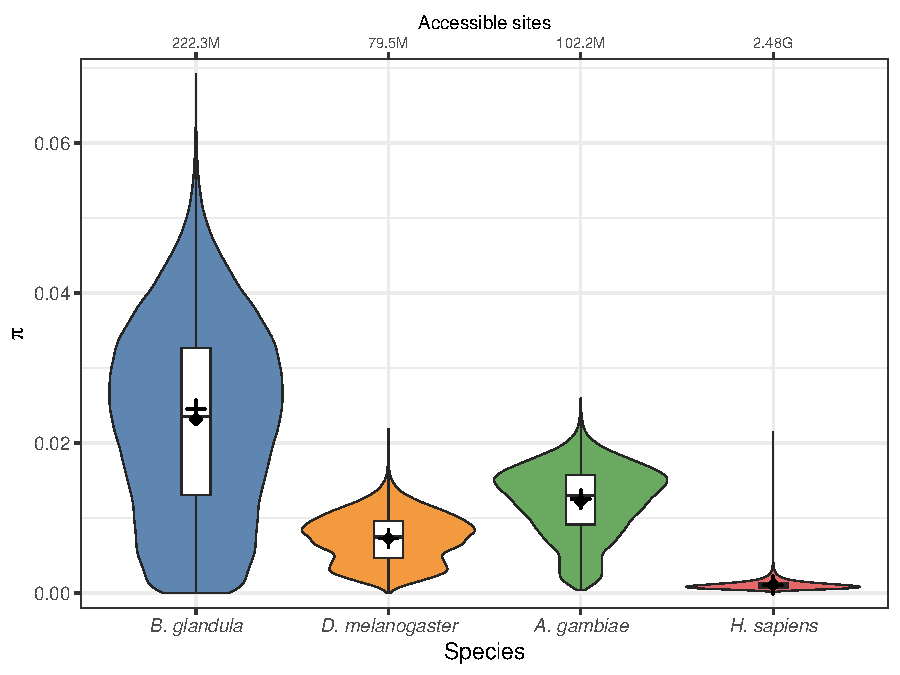
\includegraphics[width=0.9\textwidth]{figures/sups_pi_comparisons.pdf}
    \supfigurecaption{\textbf{Comparing nucleotide diversity ($\pi$) between
        barnacles and biological model systems.}
        Average $\pi$ in 10\,kbp windows between the
        Oregon Pacific acorn barnacle (\balgla{}; \texttt{BalGla}),
        Sub-Saharan populations of the fruit fly (\textit{Drosophila melanogaster};
            \texttt{DroMel}),
        malaria mosquitoes from the Central African Republic (\textit{Anopheles
            gambiae}; \texttt{AnoGam}),
        and human populations of Yoruba ancestry (\textit{Homo sapiens}; \texttt{HomSap}).
        Diamond and crosses denote the mean and pooled (sum of ratios) averages, respectively.
        Consistent with the large \Ne{} expected for \bgla{}, this barnacle population
        exhibits an average (pooled $\pi$) diversity of 0.0242.
        This is $\approx3.4\times$ higher than \textit{Drosophila} (pooled $\pi$ = 0.00728),
        $\approx2\times$ higher than \textit{An. gambiae} (pooled $\pi$ = 0.0125), and
        $\approx23\times$ higher than diverse human cohorts (pooled $\pi$ = 0.00106).}
    \label{fig:sup_pi_comp}
\end{figure}

% Pairwise correlation among different genomic feature and diversity metrics.
\begin{figure}[ht]
    \centering
    \captionsetup{width=0.95\linewidth}
    \includegraphics[width=1.0\textwidth]{figures/sups_pi_pairplot.png}
    \supfigurecaption{\textbf{Pairplot of genomic features and genetic variation
        in Oregon \balgla{}.}
        Diagonal shows the density histogram of the proportion of the genomics
        elements (e.g., CDS, lncRNA, tRNA, repeats, and introns), proportion of
        variant sites, proportion of callable sites post-filtering, and nucleotide
        diversity ($\pi$). All values computed across 10\,kbp windows. Below
        the diagonal, plots show the correlation across all pairwise comparisons.
        Red and blue lines show the linear and Loess regression, respectively.
        Above the diagonal, panels show the Spearman's rank correlation
        coefficient ($\rho$) for the given pairwise comparison.}
    \label{fig:sup_pi_pairplot}
\end{figure}

% Decay of LD with distance
\begin{figure}[ht]
    \centering
    \captionsetup{width=0.95\linewidth}
    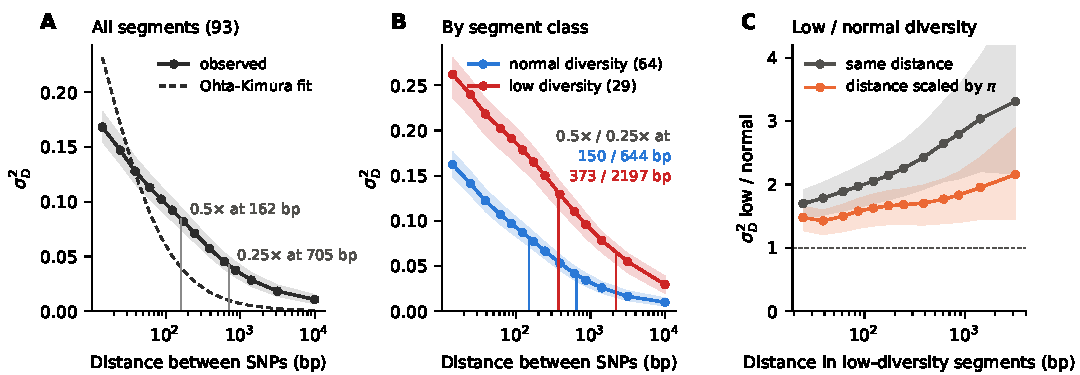
\includegraphics[width=1.0\textwidth]{figures/sups_ld_decay.pdf}
    \supfigurecaption{\textbf{Decay of linkage disequilibrium with distance in Oregon
        \balgla{}.}
        \sdsq{} is the sum of $D^{2}$ divided by the sum of $\pi_{2}$ over all
        pairs of SNPs in a distance class, calculated with the unbiased genotype
        estimators of \citet{ragsdale_unbiased_2020}. Points are at the geometric
        midpoint of each distance class. Shaded bands show 95\% confidence intervals
        from resampling segments within each class.
        \textbf{A.} All 93 segments of chromosomes 1--15. The dashed line shows the
        fitted expectation of \citet{ohta_linkage_1971} ($4N_{e}r$ = 0.14 per bp). Vertical
        lines show the distances at which \sdsq{} falls to one half and to one
        quarter of its value for SNPs 10--20\,bp apart.
        \textbf{B.} Normal-diversity (64) and low-diversity (29) segments. As in panel A,
        vertical lines show the distance at \sdsq{} falls to one half and to one
        quarter for each class.
        \textbf{C.} Ratio of \sdsq{} in low-diversity segments to \sdsq{}
        in normal-diversity segments, at the same distance (grey) and with the normal-diversity
        distances scaled by the ratio of median segment $\pi$ (0.46; orange). A ratio
        above 1 after scaling shows LD that the lower \Ne{} of the low-diversity
        segments does not explain. The first and last distance classes are not shown.}
    \label{fig:sup_ld_decay}
\end{figure}

% Diversity, divergence, and recombination
\begin{figure}[ht]
    \centering
    \captionsetup{width=0.95\linewidth}
    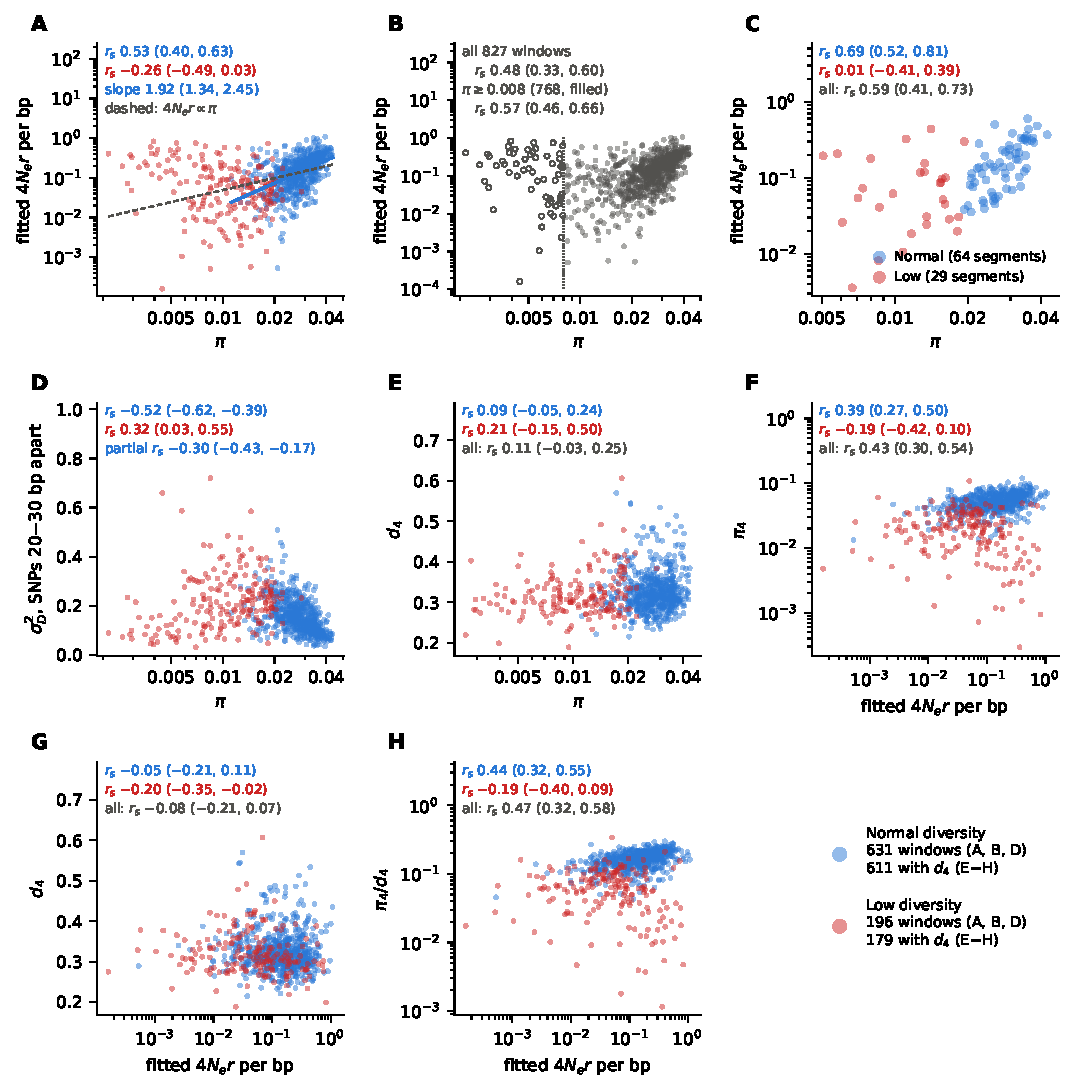
\includegraphics[width=0.95\textwidth]{figures/sups_rho_div.pdf}
    \supfigurecaption{\textbf{Diversity, divergence, and recombination in Oregon
        \balgla{}.}
        Genomic regions of normal (blue) and low (red) diversity are compared for
        metrics of genetic diversity, divergence, and recombination.
        \textbf{A.} Fitted recombination rate $\rho$ ($4N_{e}r$) against $\pi$ in
        normal and low diversity windows 1\,Mbp in length.
        The solid line is the least-squares fit of $\log 4N_{e}r$ on $\log\pi$ in
        normal windows; the dashed line is $4N_{e}r \propto \pi$.
        For all panels, $r_{s}$ denotes the Spearman's correlation coefficient with
        95\% CIs from resampling whole segments.
        \textbf{B.} Fitted $4N_{e}r$ against $\pi$ for all window pooled. The open
        circles show the 59 windows with $\pi < 0.008$.
        \textbf{C.} Fitted $4N_{e}r$ against $\pi$ for normal and low diversity
        segments (defined according to the point change analysis). Complimentary
        plot showing the slopes is shown in Figure~\ref{fig:genome_pi}E.
        \textbf{D.} \sdsq{} for SNPs 20--30\,bp apart against $\pi$ in 1\,Mbp windows.
        The partial $r_s$ count and window length constant.
        \textbf{E.} Divergence at four-fold degenerate sites ($d_4$) against $\pi$
        in 1\,Mbp windows.
        \textbf{F.} Nucleotide diversity at four-fold degenerate sites ($\pi_4$)
        against $4N_{e}r$ in 1\,Mbp windows.
        \textbf{G.} $d_4$ against $4N_{e}r$ in 1\,Mbp windows.
        \textbf{H.} $\pi_4/d_4$ against $N_{e}r$ in 1\,Mbp windows.}
    \label{fig:sup_div_rho}
\end{figure}

% Theta_W Ne
\begin{figure}[ht]
    \centering
    \captionsetup{width=0.95\linewidth}
    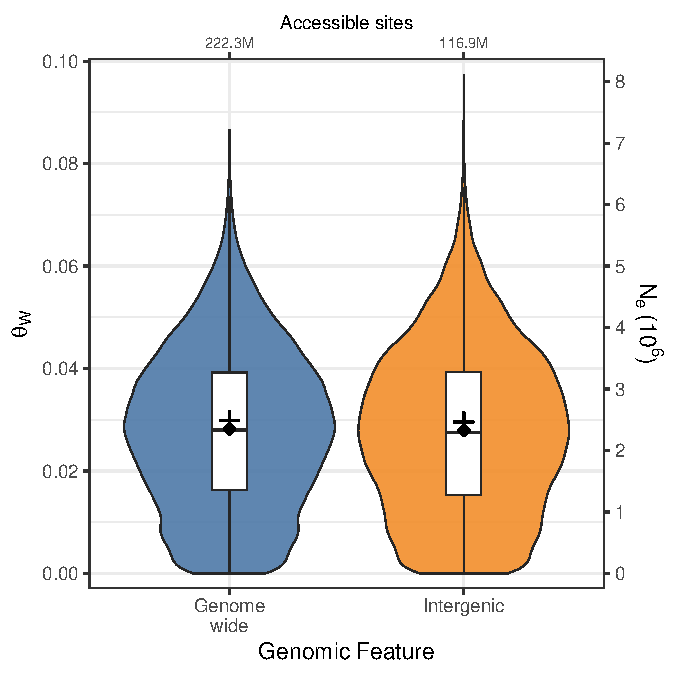
\includegraphics[width=0.8\textwidth]{figures/sups_theta_ne.pdf}
    \supfigurecaption{\textbf{Effective population (\Ne) size estimation
        of \balgla{} based on the Watterson's estimator ($\theta_\text{W}$).}
        Effective size of the population was calculated according to the
        relationship $\theta_\text{W}=4N_{e}\mu$, using a mutation rate per-base,
        per-generation ($\mu$) of $3\times10^{-9}$.
        Diamond and crosses denote the mean and pooled (sum of ratios) averages,
        respectively.
        Estimating pooled $\theta_\text{W}$ across genome-wide and intergenic sites
        in the barnacle genome yield similar long-term \Ne estimates, $2.49\times10^{6}$
        and $2.46\times10^{6}$, respectively.}
    \label{fig:sup_theta_ne}
\end{figure}

% msmc2 Ne
\begin{figure}[ht]
    \centering
    \captionsetup{width=0.95\linewidth}
    \includegraphics[width=0.9\textwidth]{figures/sups_msmc2_ne.pdf}
    \supfigurecaption{\textbf{Coalescent estimation of the effective
    population (\Ne) size estimation of \balgla{}.}
        Estimation of \Ne{} through time was done using the
        \textsc{msmc2} software, using a mutation rate per-base,
        per-generation ($\mu$) of $3\times10^{-9}$, and fixing the
        generation time ($g$) to 1.
        Each line represents the \Ne{} trajectory for each sample.
        Using just six diploid samples, and estimating only between pairs
        of unphased diploid genotypes within samples, we estimate the
        historical effective size of the population in the order of $10^{6}$
        individuals; however, we do not obtain enough resolution to resolve
        \Ne{} at recent ($<10^{5}$) time intervals.}
    \label{fig:sup_mcmc_ne}
\end{figure}

% B. glandula against published comparative data (Romiguier 2014, Galtier 2016)
\begin{figure}[ht]
    \centering
    \captionsetup{width=0.95\linewidth}
    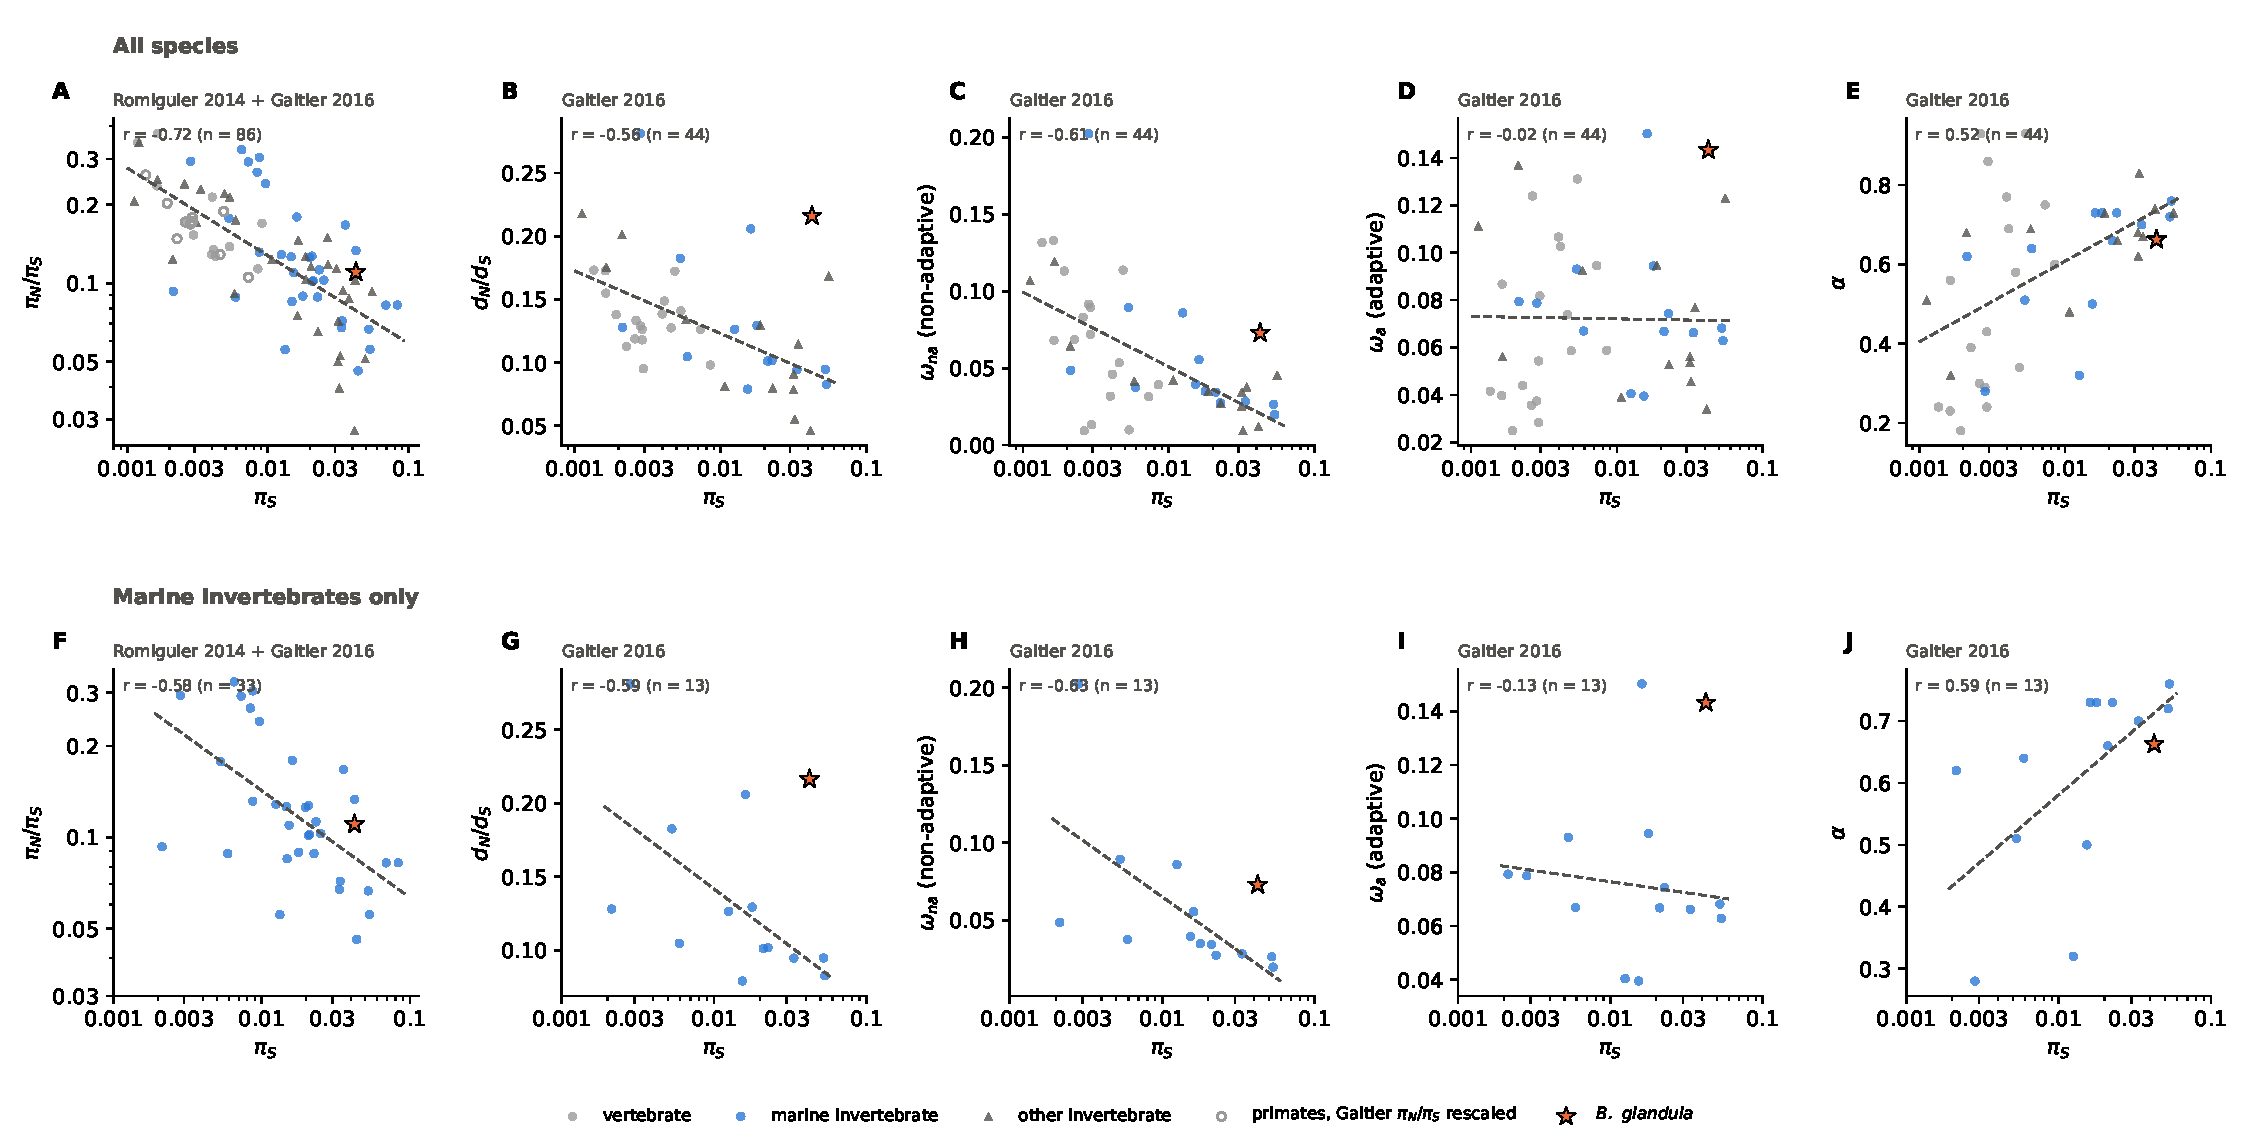
\includegraphics[width=1.0\textwidth]{figures/sups_comparative.pdf}
    \supfigurecaption{\textbf{\bgla{} in the context of published animal data.}
        Synonymous diversity ($\pi_S$) against (A, F) the ratio of non-synonymous to
        synonymous diversity ($\pi_N/\pi_S$), (B, G) \dnds{}, (C, H) the rate of
        non-adaptive amino-acid substitution ($\omega_{na}$), (D, I) the rate of
        adaptive amino-acid substitution ($\omega_{a}$), and (E, J) the proportion of
        adaptive amino-acid substitutions ($\alpha$). Top row (A--E): all species;
        bottom row (F--J): marine invertebrates only. Points are species from
        \citet{romiguier_comparative_2014} and \citet{galtier_adaptive_2016} (86 species
        for $\pi_N/\pi_S$, 44 for the other panels; 33 and 13 marine invertebrates).
        For ten primates present only in \citet{galtier_adaptive_2016}, $\pi_N/\pi_S$ was
        rescaled to the site convention of \citet{romiguier_comparative_2014} (open
        circles). $\omega_{a}$ and $\omega_{na}$ were computed per site as
        $\alpha \cdot$\dnds{} and $(1-\alpha) \cdot$\dnds{}. Dashed lines are
        least-squares fits of each variable on $\log_{10}\pi_S$; $r$ is the Pearson
        correlation. The star shows \bgla{} (all genes; $\pi_S$, $\pi_N/\pi_S$ and \dnds{}
        from the McDonald-Kreitman alignments; $\alpha$, $\omega_{a}$ and $\omega_{na}$
        from a gamma-exponential distribution of fitness effects fitted to the unfolded
        site frequency spectrum, as in \citet{galtier_adaptive_2016}; bars show 95\%
        bootstrap intervals).}
    \label{fig:sup_comparative}
\end{figure}



% Now this version matches the GENETICS submission.
% Start the edits from here.

% === Review Responses (extracted to a separate PDF by the Makefile) ===
% Revision build only. Records the absolute page number where the
% responses begin into review-responses-pagenum.txt so the Makefile can
% split main_revision.pdf into the manuscript and the response document.
\ifdefined\revisionmode
  \clearpage
  \newwrite\pageinfo
  \immediate\openout\pageinfo=review-responses-pagenum.txt
  \immediate\write\pageinfo{\thepage}
  \immediate\closeout\pageinfo
  \setcounter{page}{1}
  \label{review-responses-start}
  \nolinenumbers
  \pagestyle{plain}
  \fancyhead[L]{}
  \fancyhead[R]{}
  \begin{center}
  {\LARGE \textbf{Response to Reviewers}}\\[1em]
  {\large Large population sizes shape genome evolution in barnacles}
  \end{center}
  \vskip 2em
  % Cover letter and point-by-point reviewer responses.
% Reviewer text is verbatim from genetics_review.txt; \reply{...} blocks
% are scaffolded as TODO placeholders to be filled in during the revision.
% Wherever a change is made in the manuscript in response to a point,
% mark the manuscript line with \revpoint{R}{P} and cite it here with
% \revref (inside the matching {point}) or \revreffull{R}{P}.
%
% Reviewer labels used for \revpoint: E (editors), 1, 2.

\begin{minipage}[b]{2.5in}
  Resubmission Cover Letter \\
  {\it GENETICS} \\
  Manuscript GENETICS-2026-309883
\end{minipage}
\hfill
\begin{minipage}[b]{3.0in}
  \raggedleft
  Angel G.\ Rivera-Col\'on (on behalf of all authors) \\
  \today
\end{minipage}

\vskip 2em

\noindent
{\bf Dear Dr.\ Larracuente,}

\vskip 1em

TODO

\vskip 2em

\noindent\hspace{4em}
\begin{minipage}{4.5in}
\noindent
{\bf Sincerely,}

\vskip 2em

{\bf
  Angel G.\ Rivera-Col\'on (on behalf of all authors)
}\\
\end{minipage}

\vskip 4em

\pagebreak

%%%%%%%%%%%%%%%%%%%%%%%%%%%%%%%%%%%%%%%%%%%%%%%%%%%%%%%%%%%%%%%%%%%%%%%%%
% Editors' comments. Set up by hand rather than with \reviewersection so
% the heading doesn't read "Reviewer E"; points are tagged \revpoint{E}{P}.
\renewcommand{\thereviewer}{E}
\setcounter{point}{0}
\section*{Editors:}

\begin{itquote}
Two experts in the field have reviewed your manuscript, and the editors
have read it as well. As you can see below, both reviewers found your
manuscript well written and your system interesting, but they vary in
their view of the impact. Each reviewer has specific concerns that you
can read at the end of this e-mail. Your work clearly presents a valuable
empirical resource, however the current manuscript does not adequately
place the results in the context of other work in the field. While your
manuscript is not currently acceptable for publication in GENETICS, we
would welcome a substantially revised manuscript. Both reviewers and the
editors have comments and concerns to be addressed in a revised
manuscript.

If you do submit a revised manuscript, the revisions will need to clearly
place this work in a broader context. Please carefully consider the
comments from reviewer 2 as your revise. To be further considered by
GENETICS, the revised manuscript should emphasize how this study
contributes to our understanding of how population size interacts with
population genetic mechanisms. The revised manuscript should include
additional analyses and a major revision to the text.
\end{itquote}

\reply{TODO}

% Editor point #1
\begin{point}{} % dN/dS vs MK tension
There is no need to discuss a tension between dn/ds and the MK tests, as
you explain in the discussion that genes can experience both purifying
and positive selection.
\end{point}

\reply{TODO}

% Editor point #2
\begin{point}{} % purifying vs background selection language
Please carefully revise your language about purifying selection and
background selection, as noted by reviewers. Only use background
selection if you are are referring to the effects of purifying selection
on linked variation.
\end{point}

\reply{We agree, and we have corrected this language throughout the manuscript. We
now use ``purifying selection'' only for the direct removal of deleterious alleles at
the selected sites, and ``background selection'' only for the effect of this removal on
linked neutral variation. Two sentences used ``background selection'' for the direct
effect, and both now say ``purifying selection'' \revref, \llname{purifying_results}.
The Introduction now defines the two effects \llname{intro_linked}. In the Results, we
state that the lower diversity of whole features can come from either effect
\llname{feature_pi_linked}, and that the comparison of 0-fold and 4-fold sites in the
same codons isolates the direct effect \llname{pi0_pi4_direct}. New analyses of
linkage disequilibrium and recombination now support our statements about linked
selection; we describe them in our reply to Reviewer 1, point 1.}

% Editor point #3
\begin{point}{} % TE adaptation too speculative; TE age / size distributions
The discuss of TE adaptation is too speculative based on the data that
you present. A deeper analysis of TE age and size distributions may help
you distinguish between some of your alternative hypotheses.
\end{point}

\reply{TODO}

% Editor point #4
\begin{point}{} % focus on 4-fold pi rather than genomic pi
Don't focus so much on genomic pi. Many factors can influence this,
especially the proportion of repetitive and/or non-functional DNA in a
genome. It is much better for comparative work to focus on 4-fold
degenerate pi, as these sites are easily alignable and under weaker
selection in most lineages.
\end{point}

\reply{TODO}

% Editor point #5
\begin{point}{} % repeat-masked reference for SNP calling?
Please clarify if you used a repeat-masked reference for SNP calling, as
this may affect the level of polymorphism in non-coding regions
especially given the high repeat content of your genome.
\end{point}

\reply{TODO}

% Editor point #6
\begin{point}{} % quantitative context: 4-fold pi, Ne, MK
As noted by reviewer 2, it is important that you make an effort to
quantitatively place your findings in the context of the broader
literature addressing the relationship between 4 fold degenerate pi, Ne,
and MK tests.
\end{point}

\reply{TODO}

% Editor point #7
\begin{point}{} % correlation between dN/dS and synonymous pi
It might be interesting to look at the correlation between dN/dS and
synonymous pi. If directional selection dominates, then the correlation
might be negative.
\end{point}

\reply{TODO}

% Editor point #8
\begin{point}{} % line 47: Hill-Robertson effects
Line 47 - better stated as Hill Robertson effects
\end{point}

\reply{TODO}

% Editor point #9
\begin{point}{} % shared ortholog MK results
It may be interesting to look for shared ortholog MK results, if there
are such comparative resources.
\end{point}

\reply{TODO}

% Editor point #10
\begin{point}{} % Fig 5d: low pi regions / centromeres, physical scale
In Fig 5d, regions of low pi are indicative of centromeres exhibiting
reduced crossing-over. What is the physical scale of the phenomenon? It's
hard to tell from the figure. Are there properties of the variation or
divergence indicative of weaker selection in such regions?
\end{point}

\reply{TODO}

% Editor point #11
\begin{point}{} % lines 908-909: source of mutation rate
Lines 908-909, Please clarify where this mutation rate comes from in the
text. It appears to reference an average of 4 arthropod species rather
than one estimated based on S. balanoides data, as described in the Nunez
PNAS paper.
\end{point}

\reply{TODO}

% Editor point #12
\begin{point}{} % B. crenatus window pi from assembly heterozygosity
Regarding the B. crenatus assembly. Could one estimate a window pi from
heterozygosity in the individual used for the assembly and then
investigate whether the orthologous window pi is correlated in the two
barnacle species?
\end{point}

\reply{TODO}

% Editor point #13
\begin{point}{} % line 954: 'moderate evidence' of non-compositional ENC bias
Line 954, Be explicit about the evidence you are alluding to here
regarding the `moderate evidence' of non-compositional bias in the ENC
reduction.
\end{point}

\reply{TODO}


%%%%%%%%%%%%%%%%%%%%%%%%%%%%%%%%%%%%%%%%%%%%%%%%%%%%%%%%%%%%%%%%%%%%%%%%%
\reviewersection{1}

\begin{itquote}
This is a very strong manuscript that tackles important questions in
evolutionary biology. I agree with the authors that species with
exceptionally large Ne offer unique opportunities to investigate the
efficacy of natural selection and other fundamental evolutionary
processes, making barnacles ideal systems to tackle these questions.

The authors provide a chromosome-level genome assembly and pair this
resource with comprehensive molecular evolutionary analyses that paint a
compelling picture of the strong efficacy of selection in the species.
Overall, I am excited about this paper. I only have a few comments for
the authors to consider:
\end{itquote}

\reply{TODO}

% Reviewer 1 point #1
\begin{point}{Purifying vs.\ Background selection}
I found the evidence for efficient purifying selection in B. glandula
convincing. Yet, I got the impression that the terms ``purifying
selection'' and ``background selection'' were being used somewhat
interchangeably. To me, the manuscript makes a very strong case for the
former, whereas the latter feels harder to establish without additional
information on recombination and patterns of linkage. Since the authors
note that characterizing recombination will be focus of future work, I
encourage caution when invoking background selection in the absence of
those data.
\end{point}

\reply{We thank the reviewer for this point. We agree that we used the two terms
interchangeably, and we have corrected this throughout (see our reply to the editor,
point 2). The two sentences that gave background selection as the cause of the low
diversity in coding sequences now say purifying selection \revref,
\llname{purifying_results}. Our evidence for purifying selection is now the comparison
of 0-fold and 4-fold sites in the same codons, which linked selection cannot explain
\llname{pi0_pi4_direct}.

We also followed the reviewer's advice and examined recombination. Our sample of six
unphased individuals is too small for a recombination map, so we measured the decay of
linkage disequilibrium with the unbiased estimators of
\citet{ragsdale_unbiased_2020}. LD falls to half of its short-distance value within
161\,bp \llname{ld_decay_results}. Nucleotide diversity increases with the fitted
population recombination rate (Spearman's $\rho = 0.54$ in normal-diversity windows)
\llname{pi_rho_results}, but divergence from \textit{B. crenatus} does not
\llname{div_rho_results}. Thus, the correlation comes from variation in \Ne{} along the
genome, not from variation in the mutation rate, which is the signature of linked
selection. Background selection and recurrent selective sweeps both produce this
pattern, and our data cannot separate them. Thus, as the reviewer advises, we do not
attribute the pattern to background selection; we use the general term ``linked
selection'' \llname{disc_linked_selection}.}

% Reviewer 1 point #2
\begin{point}{Adaptive TEs}
The possibility that transposable elements contribute to adaptation in
this species is certainly intriguing. However, I would like to see a
somewhat broader discussion of non-adaptive explanations. The manuscript
paints a very consistent picture of highly efficient selection, and given
those patterns, one has to wonder why (or how) is such TE-rich genome
maintained... could there also be a role for unique dynamics of
insertion-deletion balance, or maybe heterogeneity in the recombination
landscape, etc?
\end{point}

\reply{TODO}

% Reviewer 1 point #3
\begin{point}{Codon bias}
I think the ENC/GC composition analyses are very interesting. Given the
high GC-rich nature of the genome, could GC-biased gene conversion (gBGC)
also have contributed to the observed patterns of codon usage??
\end{point}

\reply{TODO}

% Reviewer 1 point #4
\begin{point}{The balancing selection outlier}
One result that caught my attention was the candidate locus exhibiting a
strong excess of polymorphism relative to divergence. I realize this
observation is not a central focus of the manuscript, and I am not
suggesting additional analyses. However, I was curious whether the
authors have any additional thoughts about this locus. The observation
that this homolog has been implicated in osmotic stress responses makes
the result particularly intriguing, and I wonder whether the authors view
this pattern as potentially consistent with ecological processes capable
of maintaining polymorphism (e.g., intertidal zonation like that of Mpi).
I ask this simply out of curiosity.
\end{point}

\reply{TODO}


%%%%%%%%%%%%%%%%%%%%%%%%%%%%%%%%%%%%%%%%%%%%%%%%%%%%%%%%%%%%%%%%%%%%%%%%%
\reviewersection{2}

\begin{itquote}
This manuscript presents a new chromosome-level genome assembly and a
population genomic analysis of the Pacific acorn barnacle Balanus
glandula, a species characterized by very large census population sizes
and exceptionally high genetic diversity. The authors report genome-wide
nucleotide diversity exceeding 5\%, investigate the distribution of
diversity across functional categories, patterns of codon usage,
demographic history, and adaptive protein evolution. They find reduced
diversity in functional elements, as expected under purifying selection,
and infer a high contribution of positive selection to protein
divergence. Overall, the analyses are carefully conducted and the
manuscript is clearly written. B. glandula is certainly an interesting
addition to the relatively small set of species for which such high
levels of nucleotide diversity have been characterized at the
whole-genome level.

I nevertheless have two major concerns, one concerning the scope of the
study and the other its positioning with respect to the existing
literature.
\end{itquote}

\reply{TODO}


% --- Major concerns ---

% Reviewer 2 point #1
\begin{point}{Scope}
Although I found the analyses technically sound, I am not convinced that
the results provide sufficient conceptual advance.

The main novelty is essentially the detailed genomic characterization of
a single, exceptionally polymorphic species. This is valuable, but highly
polymorphic species have already been included in broad comparative
studies of genetic diversity and molecular evolution, including species
with nucleotide diversity in the same general range. The manuscript
itself cites some of this work, including Cutter's work on highly
polymorphic Caenorhabditis, but the comparative context is narrower than
it should be. Other classical examples include Ciona savignyi,
Caenorhabditis remanei and C. brenneri, and Schizophyllum commune. Large
comparative datasets such as Romiguier et al. (2014) and subsequent
studies by Galtier (on Codon Usage Bias, cited in the ms, or on adaptive
protein evolution, not cited in the ms
\url{https://doi.org/10.1371/journal.pgen.1005774}) have also included
highly polymorphic non-model species (with pi$>$5\%) and investigated the
relationships between genetic diversity, effective population size,
efficacy of purifying selection and adaptive protein evolution.

Consequently, most of the major conclusions here are consistent with
expectations and previous empirical work: very high diversity in a
species with a very large population size, stronger signatures of
purifying selection in functional sequences, and efficient adaptive
protein evolution, although Lewontin's paradox remains. I see
considerable value in documenting these patterns in B. glandula,
particularly with a high-quality genome, but less of a general conceptual
advance than suggested by the manuscript.

I therefore think that this is a good population genomic study, but one
whose contribution is primarily the genomic characterization of an
interesting non-model species.
\end{point}

\reply{TODO}

% Reviewer 2 point #2
\begin{point}{The marine population genetics literature is largely overlooked}
Another concern is the literature review and, consequently, the framing
of the study. I was quite surprised by how little the manuscript engages
with the extensive literature on genetic diversity and population
genetics of marine invertebrates.

Marine invertebrates have been central to discussions of extreme genetic
diversity since the allozyme era. High polymorphism in highly fecund
marine organisms, its relationship with census and effective population
size, and the unusual demographic processes affecting such species have
been studied for decades. In this context, I find it particularly
surprising that the work of Hedgecock and others is not discussed. The
concepts of sweepstakes reproductive success, very large variance in
reproductive success, low Ne/N ratios and, more recently, multiple-merger
coalescents and chaotic genetic patchiness are directly relevant to the
biological interpretation of the patterns reported here.

This omission matters because several observations presented as
characteristic consequences of the exceptional population size of B.
glandula have precedents in marine population genetics. For example, high
nucleotide polymorphism and its consequences for protein variation have
been investigated in marine bivalves for many years. Sauvage et al.
(2007) explicitly studied both nucleotide polymorphism and codon usage in
the Pacific oyster, reporting levels of diversity among the highest known
in animals at the time. Harrang et al. (2013) investigated the unusually
high load of non-neutral amino-acid polymorphisms in the European flat
oyster and explicitly discussed its relationship with high fecundity and
sweepstakes reproduction. More generally, marine genomes are now known to
contain extensive structural variation. Massive gene presence-absence
variation has been described in mussels (e.g. Gerdol et al. 2020), and
abundant CNVs and other structural variants have been documented in
oysters (Modak et al. 2021, Lui et al. 2025) and other marine
invertebrates (e.g. tunicates: Satou et al. 2021, lobster: Dorant et al.
2020). Thus, the genomic complexity observed here should also be
discussed in the context of this literature rather than primarily in
comparison with classical model organisms.

Similarly, mutation rate is no longer entirely unexplored in highly
fecund marine invertebrates. Direct germline mutation-rate estimates are
available, for example in sea stars (Popovic et al. 2024), and relevant
estimates also exist in tunicates. These studies are particularly
relevant to the discussion of Lewontin's paradox because they explicitly
address the respective contributions of mutation rate, census population
size and demographic history to high genetic diversity.

I am not suggesting that all these earlier studies addressed exactly the
same questions or had access to chromosome-level whole-genome data.
Clearly they did not. Rather, my concern is that the manuscript currently
creates the impression that highly polymorphic species, and particularly
highly fecund marine invertebrates, represent a largely unexplored
empirical domain. This is not the case. A more thorough treatment of this
literature would both provide a fairer historical perspective and make it
clearer what the present study genuinely adds.
\end{point}

\reply{We thank the reviewer for this point and agree that the manuscript did not
engage with the marine invertebrate literature. We have made four changes.
(1) The Introduction now places \bgla{} in this literature and in the comparative
studies that include hyperdiverse species, and no longer presents large populations as
an unexplored domain \revref.
(2) A new Discussion subsection, ``Barnacles among highly fecund marine
invertebrates'', discusses sweepstakes reproductive success, low ratios of effective to
census size, chaotic genetic patchiness and multiple-merger coalescents
\citep{hedgecock_does_1994,eldon_coalescent_2006}, and what they mean for our
estimates of \Ne{} \llname{marine_sweepstakes}.
(3) The same subsection compares our coding-sequence results with the oyster studies
the reviewer cites \llname{marine_oysters}. Unlike the flat oyster
\citep{harrang_high_2013}, \bgla{} does not carry a high load of amino-acid
polymorphism: its $\pi_N/\pi_S$ (0.11) is inside the range predicted from its $\pi_S$
across 86 animal species and across the marine invertebrates among them (new
Figure~\ref{fig:sup_comparative}). It also discusses the structural variation
documented in mussels, oysters, tunicates and lobster
\citep{gerdol_massive_2020,modak_extensive_2021,liu_bivalves_2025,
satou_chromosomal_2021,dorant_copy_2020} in relation to the complexity of the \bgla{}
genome \llname{marine_sv}.
(4) The subsection ends with the direct germline mutation rate of the crown-of-thorns
sea star \citep{popovic_high_2024}, which gives a long-term \Ne{} of about
$6\times10^{5}$ to $1.2\times10^{6}$ for \bgla{}, and with the indirect estimates
available for tunicates \citep{tsagkogeorga_population_2012}
\llname{marine_mutation_rate}.}


% --- Additional comments ---

% Reviewer 2 point #3
\begin{point}{} % codon usage: preferred vs unpreferred codons (Fop), gBGC
I am not fully convinced by the codon-usage analysis. ENC is useful as a
general measure of codon bias, but it does not directly identify which
synonymous codons are selectively preferred. In the context of this
manuscript, an analysis based on preferred versus unpreferred codons, for
example using Fop or a related measure after identifying preferred
codons, would be considerably more informative. This is particularly
important because GC3 correction alone does not fully resolve the
distinction between selection on codon usage and GC-biased gene
conversion or other GC-associated processes. Knowing whether preferred
codons are GC- or AT-ending would help discriminate among these
explanations. The literature on codon usage in highly polymorphic
species, including comparative studies by Galtier and colleagues and the
earlier work in Pacific oyster by Sauvage et al. (2007), would provide
useful context here.
\end{point}

\reply{TODO}

% Reviewer 2 point #4
\begin{point}{} % interpreting high alpha; Galtier 2016
Relatedly, I would be cautious about interpreting high alpha from
McDonald-Kreitman analyses too directly as evidence that the
exceptionally large population size of B. glandula produces unusually
strong adaptive evolution. Comparative analyses have already shown that
the relationship between effective population size and alpha is not
straightforward. In particular, Galtier (2016) found that much of the
relationship between diversity and alpha across animals could be
explained by more efficient purifying selection and a reduced
contribution of slightly deleterious substitutions, rather than by a
higher rate of adaptive substitution per se. This distinction seems
particularly relevant here.
\end{point}

\reply{TODO}

% Reviewer 2 point #5
\begin{point}{} % sweepstakes reproduction / multiple-merger coalescents
The demographic interpretation could also engage more explicitly with
reproductive biology. For a highly fecund broadcast-spawning marine
species, a Wright-Fisher model based on conventional Ne should at least
be discussed alongside sweepstakes reproduction and multiple-merger
genealogies. These processes can substantially alter the relationship
between nucleotide diversity, census size and the demographic parameters
inferred under a standard Kingman coalescent.
\end{point}

\reply{TODO}

% Reviewer 2 point #6
\begin{point}{} % connect to existing B. glandula popgen / latitudinal cline
Finally, given that B. glandula itself has a substantial population
genetic and phylogeographic literature, including work on its strong
latitudinal genetic cline, I think the manuscript could do more to
connect the new genome-wide results to what is already known about
population structure and demographic history in this particular species.
\end{point}

\reply{TODO}

% Reviewer 2 point #7
\begin{point}{Overall assessment}
This is a carefully conducted study based on a valuable new genomic
resource, and I have no major concerns about the overall quality of the
analyses. My reservations concern primarily the level of novelty claimed
and the incomplete treatment of previous work. The study provides an
interesting whole-genome characterization of an extremely polymorphic
marine species, but many of its main biological conclusions have
precedents in comparative population genomics and, especially, in the
long-standing literature on highly fecund marine invertebrates. A
substantial revision of the introduction and discussion would therefore
be necessary to place the results in their appropriate context and to
more clearly identify what is genuinely new.
\end{point}

\reply{TODO}

\fi

\end{document}
"
% which turns on line numbers and appends the point-by-point response
% document (genetics_rev1/review-responses.tex) after the supplement.
\ifdefined\revisionmode
  % Macros for reviewer responses and back-links from the response document
% to manuscript line numbers. Pattern adapted from the mkado / popgensbi
% manuscripts.
%
% Loaded only in revision mode (see the \revisionmode block in main.tex).
% Expects the lineno package to be loaded by the calling document and
% \linenumbers to be active in the manuscript body.

% Reviewer / point counters
\newcommand{\thereviewer}{}
\newcounter{point}
\setcounter{point}{0}

% Start a new reviewer block. Argument is the reviewer label
% (e.g. \reviewersection{1} or \reviewersection{AE}).
\newcommand{\reviewersection}[1]{%
  \renewcommand{\thereviewer}{#1}%
  \setcounter{point}{0}%
  \section*{Reviewer \thereviewer:}%
}

% A single review point. Argument is an optional name (often empty).
% Pattern from
% http://tex.stackexchange.com/questions/2317/latex-style-or-macro-for-detailed-response-to-referee-report
\newenvironment{point}[1]
  {\color{gray}\refstepcounter{point}\bigskip\hrule\medskip\noindent
   \slshape{\fontseries{b}\selectfont (\thereviewer.\thepoint) #1}}
  {}

\newcommand{\reply}{\normalfont\medskip\noindent\textbf{Reply}:\ }

% \revpoint{R}{P} marks a manuscript line that addresses reviewer R, point P.
% Use this in the manuscript wherever you make a change in response to a
% reviewer point so the response document can back-link to it.
\newcommand{\revpoint}[2]{\hypertarget{llineno:rev#1:#2}{\linelabel{rr:rev#1:#2}}}

% \revreffull{R}{P} renders a (page, line) reference to such a target.
\newcommand{\revreffull}[2]{{(p.\ \hyperlink{llineno:rev#1:#2}{\pageref{rr:rev#1:#2}, l.\ \lineref{rr:rev#1:#2}})}}

% \revref expands to the page/line reference for the current reviewer/point
% inside a {point} environment.
\newcommand{\revref}{\revreffull{\thereviewer}{\thepoint}\xspace}

% Named back-links: place \llabel{name} in the manuscript, refer to it
% from anywhere with \llname{name}.
\newcommand{\llabel}[1]{\hypertarget{ll:#1}{\linelabel{#1}}}
\newcommand{\llname}[1]{{(p.\ \hyperlink{ll:#1}{\pageref{#1}, l.\ \lineref{#1}})}}

% Italics-quoted block (used to set off the verbatim reviewer text).
\newenvironment{itquote}
  {\begin{quote}\color{gray}\itshape}
  {\end{quote}}

% Convenience macros
\newcommand{\rollover}{\reply{The reviewer makes an excellent point that we have missed out entirely. We have made all the changes suggested, down to the minutiae \revref.}}
\newcommand{\playdead}{\reply{The reviewer makes an excellent point. We have made an utterly trivial change \revref{}that we think deals entirely with the concern raised.}}

% lineno + amsmath fix: lineno doesn't number lines inside align/equation
% environments by default. Patch from
% http://tex.stackexchange.com/questions/43648
\ifcsname patchAmsMathEnvironmentForLineno\endcsname
\else
\newcommand*\patchAmsMathEnvironmentForLineno[1]{%
  \expandafter\let\csname old#1\expandafter\endcsname\csname #1\endcsname
  \expandafter\let\csname oldend#1\expandafter\endcsname\csname end#1\endcsname
  \renewenvironment{#1}%
    {\linenomath\csname old#1\endcsname}%
    {\csname oldend#1\endcsname\endlinenomath}}
\newcommand*\patchBothAmsMathEnvironmentsForLineno[1]{%
  \patchAmsMathEnvironmentForLineno{#1}%
  \patchAmsMathEnvironmentForLineno{#1*}}
\AtBeginDocument{%
  \patchBothAmsMathEnvironmentsForLineno{equation}%
  \patchBothAmsMathEnvironmentsForLineno{align}%
  \patchBothAmsMathEnvironmentsForLineno{flalign}%
  \patchBothAmsMathEnvironmentsForLineno{alignat}%
  \patchBothAmsMathEnvironmentsForLineno{gather}%
  \patchBothAmsMathEnvironmentsForLineno{multline}%
}
\fi

\else
  \providecommand{\revpoint}[2]{}%
  \providecommand{\revref}{}%
  \providecommand{\revreffull}[2]{}%
  \providecommand{\llabel}[1]{}%
  \providecommand{\llname}[1]{}%
\fi
% ---------------------------------------------------------------------
) by main.tex, submission_main.tex,
% and submission_sups.tex, immediately after \documentclass. This
% is done here to avoid sync issues between the main and submission
% documents. Any file-specific settings are done locally
% ============================================================

\usepackage{graphicx} % Required for inserting images
\usepackage[utf8]{inputenc}
\usepackage[letterpaper,margin=1.0in]{geometry}
%% Some formatting stuff
\usepackage{authblk}
\usepackage{fancyhdr}
\usepackage{lineno}
\usepackage{siunitx}
\sisetup{group-separator={,}, group-minimum-digits=4}
\usepackage{hyperref}
\usepackage{booktabs}
\usepackage{textgreek}
\setlength{\headheight}{13.59999pt}
\pagestyle{fancy}
\fancyhead[R]{\textbf{Rivera-Col\'{o}n \textit{et al.} 2026 - \textit{B. glandula} genome}}
% for figures
\usepackage{graphicx}
\usepackage{wrapfig}
\usepackage{breakcites}
\usepackage{nameref}
\usepackage{amsmath}
\usepackage{lipsum}
\usepackage{rotating}
\usepackage{xspace}
\usepackage{fixltx2e}
% for highlighting text. xcolor is loaded once, with dvipsnames for the named
% colors (RoyalBlue, PineGreen); a second plain load is an option clash.
\usepackage{soul}
\usepackage[dvipsnames,table]{xcolor}
% Alternating grey rows in tables. Put \shadedrows right before \begin{tabular} and
% \startshading right after the header's \midrule. Header rows stay white; the first
% data row is white and every second row after it is grey. colortbl counts \cmidrule
% lines as rows, so instead of counting header rows, shading starts at row 1000 and
% \startshading jumps the row counter there. colortbl picks each row's colour at the
% end of the row before it, so the first data row is already set to white by then and
% the counter is set to 1000 to make the second data row 1001 (odd, grey).
% Change the grey level here.
\definecolor{tablerowgrey}{gray}{0.92}
\newcommand{\shadedrows}{\rowcolors{1000}{tablerowgrey}{}}
\newcommand{\startshading}{\noalign{\global\rownum=1000\relax}}
\usepackage{caption}
\usepackage[T1]{fontenc}
\usepackage{lmodern}

% For supplemental figure and table numbering
\newcounter{supfigure}
\newcounter{suptable}

% Commands for supplemental tables and figures
\newcommand{\suptablecaption}[1]{%
    \refstepcounter{suptable}% Step forward our supplemental counter
    \renewcommand{\thetable}{S\arabic{suptable}}% Temporarily change table numbering
    \caption{#1}%
    \renewcommand{\thetable}{\arabic{table}}% Restore normal table numbering
}

\newcommand{\supfigurecaption}[1]{%
    \refstepcounter{supfigure}% Step forward our supplemental counter
    \renewcommand{\thefigure}{S\arabic{supfigure}}% Temporarily change figure numbering
    \caption{#1}%
    \renewcommand{\thefigure}{\arabic{figure}}% Restore normal figure numbering
}

% Colors for hyperlinks and other things
\hypersetup{
    colorlinks=true,
    citecolor=MidnightBlue,
    urlcolor=RoyalBlue,
    linkcolor=Blue
}
\setstcolor{Red}
\urlstyle{same}

% For the citations
\usepackage[backend=biber, style=apa, natbib=true,
    doi=true, url=true, eprint=true, isbn=false]{biblatex}
\addbibresource{references/references.bib}

% Some aliases for text
\newcommand{\dnds}{d\textsubscript{N}/d\textsubscript{S}\xspace}
\newcommand{\balgla}{\textit{Balanus glandula}\xspace}
\newcommand{\bgla}{\textit{B. glandula}\xspace}
\newcommand{\Ne}{$N_{e}$\xspace}
\newcommand{\Ks}{K\textsubscript{S}\xspace}
\newcommand{\sdsq}{$\sigma_{D}^{2}$\xspace}
\newcommand{\wrightenc}{$\text{ENC}_{exp} = 2 + s + 29/[s^{2} + (1-s)^{2}]$\xspace}
\newcommand{\comment}[1]{{\color{PineGreen} #1}}
\newcommand{\commentauth}[2]{{\color{RedViolet} \underline{#1:} #2}}

% --- Revision-mode infrastructure ------------------------------------
% Normal builds (`make`, `make submission`) leave \revisionmode undefined
% and are completely unaffected: the \revpoint / \revref / \llabel /
% \llname tags sprinkled into the sections expand to nothing.
% The revision build (`make revision`) compiles main.tex with
%   pdflatex -jobname=main_revision "\def\revisionmode{}\documentclass[11pt]{article}

% Shared packages, settings, and macros (see preamble.tex)
% ============================================================
% Shared preamble for the B. glandula genome manuscript.
%
% Included (via % ============================================================
% Shared preamble for the B. glandula genome manuscript.
%
% Included (via \input{preamble}) by main.tex, submission_main.tex,
% and submission_sups.tex, immediately after \documentclass. This
% is done here to avoid sync issues between the main and submission
% documents. Any file-specific settings are done locally
% ============================================================

\usepackage{graphicx} % Required for inserting images
\usepackage[utf8]{inputenc}
\usepackage[letterpaper,margin=1.0in]{geometry}
%% Some formatting stuff
\usepackage{authblk}
\usepackage{fancyhdr}
\usepackage{lineno}
\usepackage{siunitx}
\sisetup{group-separator={,}, group-minimum-digits=4}
\usepackage{hyperref}
\usepackage{booktabs}
\usepackage{textgreek}
\setlength{\headheight}{13.59999pt}
\pagestyle{fancy}
\fancyhead[R]{\textbf{Rivera-Col\'{o}n \textit{et al.} 2026 - \textit{B. glandula} genome}}
% for figures
\usepackage{graphicx}
\usepackage{wrapfig}
\usepackage{breakcites}
\usepackage{nameref}
\usepackage{amsmath}
\usepackage{lipsum}
\usepackage{rotating}
\usepackage{xspace}
\usepackage{fixltx2e}
% for highlighting text. xcolor is loaded once, with dvipsnames for the named
% colors (RoyalBlue, PineGreen); a second plain load is an option clash.
\usepackage{soul}
\usepackage[dvipsnames,table]{xcolor}
% Alternating grey rows in tables. Put \shadedrows right before \begin{tabular} and
% \startshading right after the header's \midrule. Header rows stay white; the first
% data row is white and every second row after it is grey. colortbl counts \cmidrule
% lines as rows, so instead of counting header rows, shading starts at row 1000 and
% \startshading jumps the row counter there. colortbl picks each row's colour at the
% end of the row before it, so the first data row is already set to white by then and
% the counter is set to 1000 to make the second data row 1001 (odd, grey).
% Change the grey level here.
\definecolor{tablerowgrey}{gray}{0.92}
\newcommand{\shadedrows}{\rowcolors{1000}{tablerowgrey}{}}
\newcommand{\startshading}{\noalign{\global\rownum=1000\relax}}
\usepackage{caption}
\usepackage[T1]{fontenc}
\usepackage{lmodern}

% For supplemental figure and table numbering
\newcounter{supfigure}
\newcounter{suptable}

% Commands for supplemental tables and figures
\newcommand{\suptablecaption}[1]{%
    \refstepcounter{suptable}% Step forward our supplemental counter
    \renewcommand{\thetable}{S\arabic{suptable}}% Temporarily change table numbering
    \caption{#1}%
    \renewcommand{\thetable}{\arabic{table}}% Restore normal table numbering
}

\newcommand{\supfigurecaption}[1]{%
    \refstepcounter{supfigure}% Step forward our supplemental counter
    \renewcommand{\thefigure}{S\arabic{supfigure}}% Temporarily change figure numbering
    \caption{#1}%
    \renewcommand{\thefigure}{\arabic{figure}}% Restore normal figure numbering
}

% Colors for hyperlinks and other things
\hypersetup{
    colorlinks=true,
    citecolor=MidnightBlue,
    urlcolor=RoyalBlue,
    linkcolor=Blue
}
\setstcolor{Red}
\urlstyle{same}

% For the citations
\usepackage[backend=biber, style=apa, natbib=true,
    doi=true, url=true, eprint=true, isbn=false]{biblatex}
\addbibresource{references/references.bib}

% Some aliases for text
\newcommand{\dnds}{d\textsubscript{N}/d\textsubscript{S}\xspace}
\newcommand{\balgla}{\textit{Balanus glandula}\xspace}
\newcommand{\bgla}{\textit{B. glandula}\xspace}
\newcommand{\Ne}{$N_{e}$\xspace}
\newcommand{\Ks}{K\textsubscript{S}\xspace}
\newcommand{\sdsq}{$\sigma_{D}^{2}$\xspace}
\newcommand{\wrightenc}{$\text{ENC}_{exp} = 2 + s + 29/[s^{2} + (1-s)^{2}]$\xspace}
\newcommand{\comment}[1]{{\color{PineGreen} #1}}
\newcommand{\commentauth}[2]{{\color{RedViolet} \underline{#1:} #2}}

% --- Revision-mode infrastructure ------------------------------------
% Normal builds (`make`, `make submission`) leave \revisionmode undefined
% and are completely unaffected: the \revpoint / \revref / \llabel /
% \llname tags sprinkled into the sections expand to nothing.
% The revision build (`make revision`) compiles main.tex with
%   pdflatex -jobname=main_revision "\def\revisionmode{}\input{main}"
% which turns on line numbers and appends the point-by-point response
% document (genetics_rev1/review-responses.tex) after the supplement.
\ifdefined\revisionmode
  \input{genetics_rev1/review-response-commands}
\else
  \providecommand{\revpoint}[2]{}%
  \providecommand{\revref}{}%
  \providecommand{\revreffull}[2]{}%
  \providecommand{\llabel}[1]{}%
  \providecommand{\llname}[1]{}%
\fi
% ---------------------------------------------------------------------
) by main.tex, submission_main.tex,
% and submission_sups.tex, immediately after \documentclass. This
% is done here to avoid sync issues between the main and submission
% documents. Any file-specific settings are done locally
% ============================================================

\usepackage{graphicx} % Required for inserting images
\usepackage[utf8]{inputenc}
\usepackage[letterpaper,margin=1.0in]{geometry}
%% Some formatting stuff
\usepackage{authblk}
\usepackage{fancyhdr}
\usepackage{lineno}
\usepackage{siunitx}
\sisetup{group-separator={,}, group-minimum-digits=4}
\usepackage{hyperref}
\usepackage{booktabs}
\usepackage{textgreek}
\setlength{\headheight}{13.59999pt}
\pagestyle{fancy}
\fancyhead[R]{\textbf{Rivera-Col\'{o}n \textit{et al.} 2026 - \textit{B. glandula} genome}}
% for figures
\usepackage{graphicx}
\usepackage{wrapfig}
\usepackage{breakcites}
\usepackage{nameref}
\usepackage{amsmath}
\usepackage{lipsum}
\usepackage{rotating}
\usepackage{xspace}
\usepackage{fixltx2e}
% for highlighting text. xcolor is loaded once, with dvipsnames for the named
% colors (RoyalBlue, PineGreen); a second plain load is an option clash.
\usepackage{soul}
\usepackage[dvipsnames,table]{xcolor}
% Alternating grey rows in tables. Put \shadedrows right before \begin{tabular} and
% \startshading right after the header's \midrule. Header rows stay white; the first
% data row is white and every second row after it is grey. colortbl counts \cmidrule
% lines as rows, so instead of counting header rows, shading starts at row 1000 and
% \startshading jumps the row counter there. colortbl picks each row's colour at the
% end of the row before it, so the first data row is already set to white by then and
% the counter is set to 1000 to make the second data row 1001 (odd, grey).
% Change the grey level here.
\definecolor{tablerowgrey}{gray}{0.92}
\newcommand{\shadedrows}{\rowcolors{1000}{tablerowgrey}{}}
\newcommand{\startshading}{\noalign{\global\rownum=1000\relax}}
\usepackage{caption}
\usepackage[T1]{fontenc}
\usepackage{lmodern}

% For supplemental figure and table numbering
\newcounter{supfigure}
\newcounter{suptable}

% Commands for supplemental tables and figures
\newcommand{\suptablecaption}[1]{%
    \refstepcounter{suptable}% Step forward our supplemental counter
    \renewcommand{\thetable}{S\arabic{suptable}}% Temporarily change table numbering
    \caption{#1}%
    \renewcommand{\thetable}{\arabic{table}}% Restore normal table numbering
}

\newcommand{\supfigurecaption}[1]{%
    \refstepcounter{supfigure}% Step forward our supplemental counter
    \renewcommand{\thefigure}{S\arabic{supfigure}}% Temporarily change figure numbering
    \caption{#1}%
    \renewcommand{\thefigure}{\arabic{figure}}% Restore normal figure numbering
}

% Colors for hyperlinks and other things
\hypersetup{
    colorlinks=true,
    citecolor=MidnightBlue,
    urlcolor=RoyalBlue,
    linkcolor=Blue
}
\setstcolor{Red}
\urlstyle{same}

% For the citations
\usepackage[backend=biber, style=apa, natbib=true,
    doi=true, url=true, eprint=true, isbn=false]{biblatex}
\addbibresource{references/references.bib}

% Some aliases for text
\newcommand{\dnds}{d\textsubscript{N}/d\textsubscript{S}\xspace}
\newcommand{\balgla}{\textit{Balanus glandula}\xspace}
\newcommand{\bgla}{\textit{B. glandula}\xspace}
\newcommand{\Ne}{$N_{e}$\xspace}
\newcommand{\Ks}{K\textsubscript{S}\xspace}
\newcommand{\sdsq}{$\sigma_{D}^{2}$\xspace}
\newcommand{\wrightenc}{$\text{ENC}_{exp} = 2 + s + 29/[s^{2} + (1-s)^{2}]$\xspace}
\newcommand{\comment}[1]{{\color{PineGreen} #1}}
\newcommand{\commentauth}[2]{{\color{RedViolet} \underline{#1:} #2}}

% --- Revision-mode infrastructure ------------------------------------
% Normal builds (`make`, `make submission`) leave \revisionmode undefined
% and are completely unaffected: the \revpoint / \revref / \llabel /
% \llname tags sprinkled into the sections expand to nothing.
% The revision build (`make revision`) compiles main.tex with
%   pdflatex -jobname=main_revision "\def\revisionmode{}\documentclass[11pt]{article}

% Shared packages, settings, and macros (see preamble.tex)
\input{preamble}

% Shared title, authors, and affiliations (see title_authors.tex)
\input{title_authors}

\begin{document}

\maketitle

% Line numbers in the manuscript body for reviewer reference (revision only).
\ifdefined\revisionmode\linenumbers\fi

\input{sections/abstract}

%% Main sections
\input{sections/introduction}
\input{sections/methods}
\input{sections/results}
\input{sections/discussion}
\input{sections/conclusion}
\input{sections/data_avail.tex}
\input{sections/acknowledgments}
\input{sections/author_contributions}

% Clear a new page for the bibliography
\clearpage

\printbibliography

% Supplements
\clearpage

\fancyhead[L]{\textit{SUPPLEMENTS}}

\input{sections/supplement_methods}

\clearpage

\input{sections/supplement_tables}

\clearpage

\input{sections/supplement_figures}

% Now this version matches the GENETICS submission.
% Start the edits from here.

% === Review Responses (extracted to a separate PDF by the Makefile) ===
% Revision build only. Records the absolute page number where the
% responses begin into review-responses-pagenum.txt so the Makefile can
% split main_revision.pdf into the manuscript and the response document.
\ifdefined\revisionmode
  \clearpage
  \newwrite\pageinfo
  \immediate\openout\pageinfo=review-responses-pagenum.txt
  \immediate\write\pageinfo{\thepage}
  \immediate\closeout\pageinfo
  \setcounter{page}{1}
  \label{review-responses-start}
  \nolinenumbers
  \pagestyle{plain}
  \fancyhead[L]{}
  \fancyhead[R]{}
  \begin{center}
  {\LARGE \textbf{Response to Reviewers}}\\[1em]
  {\large Large population sizes shape genome evolution in barnacles}
  \end{center}
  \vskip 2em
  \input{genetics_rev1/review-responses}
\fi

\end{document}
"
% which turns on line numbers and appends the point-by-point response
% document (genetics_rev1/review-responses.tex) after the supplement.
\ifdefined\revisionmode
  % Macros for reviewer responses and back-links from the response document
% to manuscript line numbers. Pattern adapted from the mkado / popgensbi
% manuscripts.
%
% Loaded only in revision mode (see the \revisionmode block in main.tex).
% Expects the lineno package to be loaded by the calling document and
% \linenumbers to be active in the manuscript body.

% Reviewer / point counters
\newcommand{\thereviewer}{}
\newcounter{point}
\setcounter{point}{0}

% Start a new reviewer block. Argument is the reviewer label
% (e.g. \reviewersection{1} or \reviewersection{AE}).
\newcommand{\reviewersection}[1]{%
  \renewcommand{\thereviewer}{#1}%
  \setcounter{point}{0}%
  \section*{Reviewer \thereviewer:}%
}

% A single review point. Argument is an optional name (often empty).
% Pattern from
% http://tex.stackexchange.com/questions/2317/latex-style-or-macro-for-detailed-response-to-referee-report
\newenvironment{point}[1]
  {\color{gray}\refstepcounter{point}\bigskip\hrule\medskip\noindent
   \slshape{\fontseries{b}\selectfont (\thereviewer.\thepoint) #1}}
  {}

\newcommand{\reply}{\normalfont\medskip\noindent\textbf{Reply}:\ }

% \revpoint{R}{P} marks a manuscript line that addresses reviewer R, point P.
% Use this in the manuscript wherever you make a change in response to a
% reviewer point so the response document can back-link to it.
\newcommand{\revpoint}[2]{\hypertarget{llineno:rev#1:#2}{\linelabel{rr:rev#1:#2}}}

% \revreffull{R}{P} renders a (page, line) reference to such a target.
\newcommand{\revreffull}[2]{{(p.\ \hyperlink{llineno:rev#1:#2}{\pageref{rr:rev#1:#2}, l.\ \lineref{rr:rev#1:#2}})}}

% \revref expands to the page/line reference for the current reviewer/point
% inside a {point} environment.
\newcommand{\revref}{\revreffull{\thereviewer}{\thepoint}\xspace}

% Named back-links: place \llabel{name} in the manuscript, refer to it
% from anywhere with \llname{name}.
\newcommand{\llabel}[1]{\hypertarget{ll:#1}{\linelabel{#1}}}
\newcommand{\llname}[1]{{(p.\ \hyperlink{ll:#1}{\pageref{#1}, l.\ \lineref{#1}})}}

% Italics-quoted block (used to set off the verbatim reviewer text).
\newenvironment{itquote}
  {\begin{quote}\color{gray}\itshape}
  {\end{quote}}

% Convenience macros
\newcommand{\rollover}{\reply{The reviewer makes an excellent point that we have missed out entirely. We have made all the changes suggested, down to the minutiae \revref.}}
\newcommand{\playdead}{\reply{The reviewer makes an excellent point. We have made an utterly trivial change \revref{}that we think deals entirely with the concern raised.}}

% lineno + amsmath fix: lineno doesn't number lines inside align/equation
% environments by default. Patch from
% http://tex.stackexchange.com/questions/43648
\ifcsname patchAmsMathEnvironmentForLineno\endcsname
\else
\newcommand*\patchAmsMathEnvironmentForLineno[1]{%
  \expandafter\let\csname old#1\expandafter\endcsname\csname #1\endcsname
  \expandafter\let\csname oldend#1\expandafter\endcsname\csname end#1\endcsname
  \renewenvironment{#1}%
    {\linenomath\csname old#1\endcsname}%
    {\csname oldend#1\endcsname\endlinenomath}}
\newcommand*\patchBothAmsMathEnvironmentsForLineno[1]{%
  \patchAmsMathEnvironmentForLineno{#1}%
  \patchAmsMathEnvironmentForLineno{#1*}}
\AtBeginDocument{%
  \patchBothAmsMathEnvironmentsForLineno{equation}%
  \patchBothAmsMathEnvironmentsForLineno{align}%
  \patchBothAmsMathEnvironmentsForLineno{flalign}%
  \patchBothAmsMathEnvironmentsForLineno{alignat}%
  \patchBothAmsMathEnvironmentsForLineno{gather}%
  \patchBothAmsMathEnvironmentsForLineno{multline}%
}
\fi

\else
  \providecommand{\revpoint}[2]{}%
  \providecommand{\revref}{}%
  \providecommand{\revreffull}[2]{}%
  \providecommand{\llabel}[1]{}%
  \providecommand{\llname}[1]{}%
\fi
% ---------------------------------------------------------------------


% Shared title, authors, and affiliations (see title_authors.tex)
% Shared title, author list, and affiliations, included by main.tex,
% submission_main.tex, and submission_sups.tex so the three documents cannot
% drift apart. Edit here only.
%
% Input this after % ============================================================
% Shared preamble for the B. glandula genome manuscript.
%
% Included (via \input{preamble}) by main.tex, submission_main.tex,
% and submission_sups.tex, immediately after \documentclass. This
% is done here to avoid sync issues between the main and submission
% documents. Any file-specific settings are done locally
% ============================================================

\usepackage{graphicx} % Required for inserting images
\usepackage[utf8]{inputenc}
\usepackage[letterpaper,margin=1.0in]{geometry}
%% Some formatting stuff
\usepackage{authblk}
\usepackage{fancyhdr}
\usepackage{lineno}
\usepackage{siunitx}
\sisetup{group-separator={,}, group-minimum-digits=4}
\usepackage{hyperref}
\usepackage{booktabs}
\usepackage{textgreek}
\setlength{\headheight}{13.59999pt}
\pagestyle{fancy}
\fancyhead[R]{\textbf{Rivera-Col\'{o}n \textit{et al.} 2026 - \textit{B. glandula} genome}}
% for figures
\usepackage{graphicx}
\usepackage{wrapfig}
\usepackage{breakcites}
\usepackage{nameref}
\usepackage{amsmath}
\usepackage{lipsum}
\usepackage{rotating}
\usepackage{xspace}
\usepackage{fixltx2e}
% for highlighting text. xcolor is loaded once, with dvipsnames for the named
% colors (RoyalBlue, PineGreen); a second plain load is an option clash.
\usepackage{soul}
\usepackage[dvipsnames,table]{xcolor}
% Alternating grey rows in tables. Put \shadedrows right before \begin{tabular} and
% \startshading right after the header's \midrule. Header rows stay white; the first
% data row is white and every second row after it is grey. colortbl counts \cmidrule
% lines as rows, so instead of counting header rows, shading starts at row 1000 and
% \startshading jumps the row counter there. colortbl picks each row's colour at the
% end of the row before it, so the first data row is already set to white by then and
% the counter is set to 1000 to make the second data row 1001 (odd, grey).
% Change the grey level here.
\definecolor{tablerowgrey}{gray}{0.92}
\newcommand{\shadedrows}{\rowcolors{1000}{tablerowgrey}{}}
\newcommand{\startshading}{\noalign{\global\rownum=1000\relax}}
\usepackage{caption}
\usepackage[T1]{fontenc}
\usepackage{lmodern}

% For supplemental figure and table numbering
\newcounter{supfigure}
\newcounter{suptable}

% Commands for supplemental tables and figures
\newcommand{\suptablecaption}[1]{%
    \refstepcounter{suptable}% Step forward our supplemental counter
    \renewcommand{\thetable}{S\arabic{suptable}}% Temporarily change table numbering
    \caption{#1}%
    \renewcommand{\thetable}{\arabic{table}}% Restore normal table numbering
}

\newcommand{\supfigurecaption}[1]{%
    \refstepcounter{supfigure}% Step forward our supplemental counter
    \renewcommand{\thefigure}{S\arabic{supfigure}}% Temporarily change figure numbering
    \caption{#1}%
    \renewcommand{\thefigure}{\arabic{figure}}% Restore normal figure numbering
}

% Colors for hyperlinks and other things
\hypersetup{
    colorlinks=true,
    citecolor=MidnightBlue,
    urlcolor=RoyalBlue,
    linkcolor=Blue
}
\setstcolor{Red}
\urlstyle{same}

% For the citations
\usepackage[backend=biber, style=apa, natbib=true,
    doi=true, url=true, eprint=true, isbn=false]{biblatex}
\addbibresource{references/references.bib}

% Some aliases for text
\newcommand{\dnds}{d\textsubscript{N}/d\textsubscript{S}\xspace}
\newcommand{\balgla}{\textit{Balanus glandula}\xspace}
\newcommand{\bgla}{\textit{B. glandula}\xspace}
\newcommand{\Ne}{$N_{e}$\xspace}
\newcommand{\Ks}{K\textsubscript{S}\xspace}
\newcommand{\sdsq}{$\sigma_{D}^{2}$\xspace}
\newcommand{\wrightenc}{$\text{ENC}_{exp} = 2 + s + 29/[s^{2} + (1-s)^{2}]$\xspace}
\newcommand{\comment}[1]{{\color{PineGreen} #1}}
\newcommand{\commentauth}[2]{{\color{RedViolet} \underline{#1:} #2}}

% --- Revision-mode infrastructure ------------------------------------
% Normal builds (`make`, `make submission`) leave \revisionmode undefined
% and are completely unaffected: the \revpoint / \revref / \llabel /
% \llname tags sprinkled into the sections expand to nothing.
% The revision build (`make revision`) compiles main.tex with
%   pdflatex -jobname=main_revision "\def\revisionmode{}\input{main}"
% which turns on line numbers and appends the point-by-point response
% document (genetics_rev1/review-responses.tex) after the supplement.
\ifdefined\revisionmode
  \input{genetics_rev1/review-response-commands}
\else
  \providecommand{\revpoint}[2]{}%
  \providecommand{\revref}{}%
  \providecommand{\revreffull}[2]{}%
  \providecommand{\llabel}[1]{}%
  \providecommand{\llname}[1]{}%
\fi
% ---------------------------------------------------------------------
: the affiliations need authblk and the
% corresponding-author line needs hyperref.
%
% The title text is also kept on its own in \mstitle, so a document can build a
% variant of it without repeating the wording -- submission_sups.tex prefixes it
% with "Supplementary information for:" by redefining \title after the \input.

\newcommand{\mstitle}{Large population sizes shape genome evolution in barnacles}
\title{\mstitle}

\author[1*]{Angel G. Rivera-Col\'{o}n}
\author[1]{Scott T. Small}
\author[2,3]{Erin Jezuit}
\author[4,5]{John P. Wares}
\author[1]{\mbox{Andrew D. Kern}}

\affil[1]{\small{Department of Biology, Institute of Ecology and Evolution, University of Oregon, USA}}
\affil[2]{\small{Department of Biology, Institute of Molecular Biology, University of Oregon, USA}}
\affil[3]{\small{Department of Biology, Oregon Institute of Marine Biology, University of Oregon, USA}}
\affil[4]{\small{Odum School of Ecology, University of Georgia, USA}}
\affil[5]{\small{Department of Genetics, University of Georgia, USA}}
\affil[*]{\small{Address correspondence to: \href{mailto:ariverac@uoregon.edu}{ariverac@uoregon.edu}}}


\begin{document}

\maketitle

% Line numbers in the manuscript body for reviewer reference (revision only).
\ifdefined\revisionmode\linenumbers\fi

% Having a shared abstract here because before the main and submission versions
% of the document were not in sync. This should avoid this issue in the future.
\begin{abstract}

Population size is a key factor underlying the mode and tempo of evolution,
particularly as it relates to the strength of selection and drift.
While the mechanisms underlying the interactions between population size
and selection have been studied in population genetics for over a century, empirical
knowledge of these dynamics has been limited to species with small-to-moderate
historical population sizes. This gap in knowledge highlights the need for empirical
studies in systems with historically large population sizes and elevated diversity.
The Pacific acorn barnacle (\balgla) presents an exceptional model to study evolution
in extremely large populations, exhibiting census sizes often exceeding the tens of
thousands of individuals per square meter.
We generated a new chromosome-level genome assembly for this species, which we leverage
in one of the first large-scale genomic analyses in this system.
This assembly reveals a highly polymorphic genome with over 3\% heterozygosity.
At a population level, \bgla{} exhibits extreme levels of polymorphism,
with nucleotide diversity surpassing 5\%\comment{[Old pixy value; pixy dropped invariant sites with QUAL $<$ 30, so $\pi$ and $\theta_W$ are about 2$\times$ too high. Corrected genome-wide $\pi$ = 0.024 (\texttt{pg\_gpu\_stats}). Update.]} genome-wide in just a small collection of
individuals.
Nucleotide diversity is lower in functional elements, including both coding and
non-coding sequences.
In protein-coding sequences, diversity at non-synonymous sites is much lower than at
synonymous sites in the same codons, which shows strong purifying selection.
Diversity also increases with the population recombination rate, which shows that
selection at linked sites reduces diversity along the genome.
At the same time, McDonald-Kreitman tests reveal that the majority of non-synonymous
substitutions between barnacle species were driven by positive selection, consistent
with the expected increase in the efficacy of selection in large populations.
These remarkable levels of diversity set \bgla{} as a unique model for the study of
evolution at extreme demographic scales and highlights the importance of testing
evolutionary theory across a wide variety of empirical systems.

\end{abstract}


%% Main sections
\section*{Introduction}

The size of a population is a key factor mediating the mode and tempo of evolution,
particularly as it relates to the strength of stochastic versus deterministic
evolutionary processes \citep{kimura_mutation_1963,gillespie_genetic_2000}.
Population genetics theory predicts that selection is less efficacious in small populations
\citep{charlesworth_effective_2009,gravel_when_2016}, resulting in reduced genetic
diversity from genetic drift and an increase in genetic load due to the accumulation
of deleterious mutations \citep{lande_risk_1994,lynch_mutation_1995,dussex_purging_2023}.
These dynamics have been extensively observed in natural populations, e.g., the
increase in genetic load in humans as a function of their geographic distance to more
diverse groups in sub-Saharan Africa \citep{henn_distance_2016} and the increase in
genetic load and inbreeding depression in small populations of conservation concern
\citep{lande_genetics_1988,westemeier_prairiechicken_1998,frankham_genetics_2005,
kardos_inbreeding_2023}, empirically supporting the theoretical expectations.
\vspace{0.1cm}

In contrast, evolution in large populations is thought to be primarily mediated by
deterministic processes due to an increase in the efficacy of selection
\citep{charlesworth_effective_2009,gravel_when_2016,lanfear_population_2014}.
The dynamics of selection in large populations are expected to produce patterns
\comment{Hill Robertson?}
such as clonal-interference effects driven by soft sweeps and recurrent mutation
\citep{park_clonal_2007,weissman_rate_2014}, as well as the loss of genetic
diversity through the hitchhiking effect \citep{smith_hitch-hiking_1974}.
In sufficiently large populations, this process is predicted to be a primary driver
of stochastic diversity loss \citep{gillespie_genetic_2000,gillespie_role_1999}.
\llabel{intro_linked}Purifying selection has a similar linked effect.
Its direct effect is the removal of deleterious alleles at the selected sites.
Its linked effect, background selection, is the loss of neutral diversity at sites
linked to the selected sites \citep{charlesworth_effect_1993}.
Both forms of linked selection, selective sweeps and background selection, reduce
diversity most where recombination is low \citep{begun_levels_1992}.
\revpoint{2}{2}Highly fecund marine invertebrates have long been central to this question.
Since the allozyme era they have been among the most polymorphic animals known,
and the links between their diversity and their
reproductive biology have been studied for decades \citep{hedgecock_does_1994}.
Hyperdiverse species are also part of broad comparative studies of diversity and
molecular evolution \citep{romiguier_comparative_2014,galtier_adaptive_2016,
galtier_codon_2018}, and several have been studied in detail, including the sea squirt
\textit{Ciona savignyi} \citep{small_extreme_2007}, the nematodes
\textit{Caenorhabditis remanei} and \textit{C. brenneri}
\citep{cutter_high_2006,dey_molecular_2013}, and the fungus \textit{Schizophyllum commune}
\citep{baranova_extraordinary_2015}; other studies of genetic diversity and the
mechanisms of evolution in large populations include
\citet{ag1000g,teterina_pervasive_2025,anderson_population_2017,braso-vives_highly_2026}.
However, most of this work, particularly that focused on marine organisms,
 used tens of loci, transcriptomes, or a single genome, and
chromosome-level analyses of population samples in highly fecund marine invertebrates
remain few.
Instead, empirical work on this subject has mainly focused on eukaryotic species with
small-to-moderate historical population sizes \citep{cutter_molecular_2013,
leffler_revisiting_2012,buffalo_quantifying_2021}, limiting our capacity to observe
these evolutionary dynamics at demographic extremes.
This gap highlights the need for empirical studies in systems with historically large
population sizes and elevated levels of genetic polymorphism.
\vspace{0.1cm}

The Pacific acorn barnacle (\balgla{}; Balanidae) presents an exceptional model for
studying the dynamics and mechanisms of evolution in large populations.
This species is widespread across the Pacific intertidal of North America, from Baja
California to Alaska, where it can reach densities of $10^4$ of individuals per square
meter \citep{menge_recruitment_2000}.
Like most acorn barnacles, \bgla{} is a sessile, simultaneous hermaphrodite that
reproduces through cross-fertilization, mating with its neighbors via pseudo-copulation;
even isolated individuals, beyond the reach of any mate, can produce outcrossed broods
by capturing water-borne sperm \citep{barazandeh_spermcast_2014}.
Individuals of this species can be long-lived ($8 \mbox{--} 10$ years;
\citealp{newman_cirripedia_1980}) and show high fecundity, with 2--6 broods per year
\citep{hoeg_cirripedia_1987,hines_reproduction_1978}, brood sizes of $10^3 \mbox{--} 10^4$
embryos \citep{barnes_general_1956}, and a reproductive output of $\approx10^3$ nauplius
larvae per individual \citep{leslie_barnacle_2005}.
Additionally, \bgla{} displays high dispersive potential.
Nauplius larvae feed and develop in the plankton for a period of weeks before settling
\citep{brown_larvae_1985,pfeiffer-hoyt_modeling_2005}, leading to their dispersal up
to hundreds of kilometers \citep{sotka_larvae_2006,sotka_strong_2004}.
This combination of high fecundity, outcrossing, and long-lived planktonic larvae
capable of long-distance dispersal, together with these enormous census sizes, is
consistent with very large effective population sizes, making \bgla{} an ideal system
for testing theoretical predictions about selection and drift in large populations.
\vspace{0.1cm}

This species has been the focus of extensive ecological and genetic research. Prior work
has linked environmental factors to variation in development, recruitment, dispersal,
and reproduction \citep{berger_spatial_2006,berger_reproduction_2009,
barshis_coastal_2011,pfeiffer-hoyt_modeling_2005,schubart_recruitment_1995}, and
substantial effort has characterized the spatial population structure of \bgla{}
along the Pacific coast, particularly a steep genetic cline on the coast of
California that separates northern and southern populations
\citep{sotka_strong_2004,wares_diversification_2005,wares_maintenance_2019,
wares_diversity_2021}.
Yet, \bgla{} remains genomically understudied.
Previous research has been limited to a handful of nuclear and mitochondrial markers,
with the most extensive study employing reduced representation sequencing in the
absence of a reference genome \citep{wares_diversity_2021}.
Moreover, while two reference assemblies for \bgla{} exist in public databases, both are
highly fragmented and likely incomplete, which limits their use when studying genome-wide
patterns of diversity and selection in this system.
\vspace{0.1cm}

Most publicly available barnacle assemblies suffer from similar limitations, presumably
due to the difficulty of assembling highly polymorphic genomes from short reads
\citep{vinson_assembly_2005,kajitani_efficient_2014}.
Despite this limitation, a handful of chromosome-level assemblies have been recently
generated for several barnacle species \citep{han_new_2024,bishop_genome_2025,
bernot_chromosome-level_2022,carlson_reference_2025,blaxter_genome_2023}.
Yet, these genomes largely belong to evolutionarily or geographically distant species.
While useful for the long-term comparisons we perform here, their evolutionary distance
limits the utility of these resources for studies in \bgla{}.
This drives the need for high-quality assemblies of both evolutionarily
closely related species, which could serve as outgroups for recent evolutionary
comparisons, and co-localized species, which enable the study of ecological factors
maintaining diversity in this system.
\vspace{0.1cm}

Work in other barnacle species has revealed substantial levels of genetic diversity
\citep{alm_rosenblad_genomic_2021}, in accordance with the expectation of very large
effective populations, and complex patterns of selection at remarkably small spatial
scales.
The best-characterized example is the balanced polymorphism at the mannose-6-phosphate
isomerase (\textit{Mpi}) locus in the northern acorn barnacle \textit{Semibalanus
balanoides}, which segregates across intertidal environments
\citep{schmidt_environmental_2000,nunez_footprints_2020}.
Building on this single-locus work, whole-genome pooled resequencing across intertidal
microhabitats has shown that spatially varying selection extends beyond \textit{Mpi},
leaving genomic signatures of adaptation to environmental heterogeneity at loci
throughout the \textit{S. balanoides} genome \citep{nunez_tides_2021}.
These studies demonstrate that selection can structure barnacle genetic variation over
just meters of tidal height; however, such genome-wide inference has so far relied on
a fragmented draft assembly in a single species, and the landscape of diversity and
selection remains uncharacterized across most of the barnacle tree, including \bgla{}.
\vspace{0.1cm}

In this work we start addressing the need for empirical systems to study evolution in
large populations by generating a high-quality, chromosome-level assembly for the Pacific
acorn barnacle.
We additionally generate a draft assembly for its congener, the wrinkled barnacle
\textit{Balanus crenatus}, providing a closely related outgroup for divergence-based analyses.
We use these assemblies to perform whole-genome comparative analyses, revealing conservation
in genome architecture across 165 million years of barnacle evolution.
We further conduct the first genome-wide assessment of genetic variation in this system,
uncovering extreme levels ($>5\%$)\comment{[Old pixy value; pixy dropped invariant sites with QUAL $<$ 30, so $\pi$ and $\theta_W$ are about 2$\times$ too high. Corrected: genome-wide $\pi$ = 0.024, 4-fold $\pi$ = 0.043 (\texttt{pg\_gpu\_stats}). Update.]} of nucleotide diversity, with over 20 million SNPs
observed in just six individuals.
Consistent with theoretical expectations, we observe reduced diversity in protein-coding
sequences, reflecting strong \revpoint{E}{2}\revpoint{1}{1}purifying selection and functional
constraints.
McDonald-Kreitman tests further reveal that the majority of non-synonymous substitutions
between species were driven by positive selection, as expected when selection is highly
efficacious in large populations.
In addition to providing high-quality genomic resources for a genomically understudied
group, our assemblies lay the groundwork for future work in \bgla{} and other barnacles as
models for the study of evolution in large, hyperpolymorphic populations.
\vspace{0.1cm}


\section*{Materials and Methods}

\subsection*{DNA and RNA sequencing}

\subsubsection*{High-molecular weight DNA and PacBio sequencing}

For genome sequencing using PacBio Hi-Fi reads, we sampled several \balgla{}
individuals from the docks in the Oregon Institute of Marine Biology, in Charleston,
Oregon, USA (43.346 N, 124.325 W). Individuals were hand collected at low tide in
February 2023. High-molecular weight (HMW) DNA was extracted using the PacBio Nanobind
tissue kit (PacBio) and quality checked using
fluorometric quantification of concentration (Qubit; Invitrogen) and fragment
length distribution (Fragment Analyzer; Advanced Analytical). The extracted DNA
of a single individual was sequenced on three SMRTcells of a PacBio Sequel
II machine at the University of Oregon's Genomics and Cell Characterization Core
Facility (GC3F). These three sequencing runs yielded a total of 5.93 million
reads with a read N50 of 12.4\,kbp.

\subsubsection*{Chromosome conformation capture}

We generated chromosome conformation capture (Hi-C) libraries from a \textit{B.
glandula} individual collected from Cape Perpetua, Oregon, USA (44.279 N, 124.112
W) in August 2023. Library construction was performed by Phase Genomics, Inc.
The final library was sequenced on an Illumina NovaSeq6000 S4 lane at the University
of Oregon's GC3F, yielding 414.3 million read pairs.

\subsubsection*{ONT ultra-long read sequencing}

The HMW DNA from a \bgla{} individual collected from Cape Perpetua,
Oregon, USA in August 2023 was extracted using the QIAGEN Genomic-Tips 20/G kit,
processed using an Ultra-Long DNA Sequencing Kit and sequenced
using an Oxford Nanopore (ONT) GridION at the University of Oregon's GC3F. This
library yielded 387 thousand ONT reads with a read N50 of 42.7\,kbp.

\subsubsection*{RNA sequencing}

RNA was extracted from a \bgla{} individual collected from Cape
Perpetua, Oregon, USA in August 2023. For RNAseq, RNA was extracted from the
testes and cirri, and sequenced on an Illumina NovaSeq6000 S4 lane at the University
of Oregon's GC3F, resulting in 276.8 million read pairs across both tissue types.
The same extracted RNA was used for Iso-Seq, preparing libraries from cirri and testes,
and sequenced on a PacBio SMRTcell at the University of Oregon's GC3F. The
testes library yielded 1.4 million reads with a read N50 of 1.4\,kbp, while the
cirri library yielded 1.9 million reads with a read N50 of 1.5\,kbp. In total,
the two libraries combined resulted in 3.3 million reads, with a read N50 of
1.5\,kbp.

\subsubsection*{Whole-genome shotgun sequencing}

Genomic DNA was extracted from eight \bgla{} individuals collected
from Cape Perpetua, Oregon, USA in August 2023 using the QIAGEN Genomic-Tips
20/G kit. The extracted DNA was processed using the Illumina TrueSeq library
kit and sequenced, pooled along with other samples, on two Illumina NovaSeq6000
S4 2 $\times$ 150\,bp lanes at the University of Oregon's GC3F. Across both lanes,
the sequencing process yielded 1.97 billion reads across the eight individuals,
an average of 246.3 million reads per individual. In total, these individuals
were sequenced at an estimated depth of $\approx$ 60x.

\subsection*{Genome assembly}\label{sec:methods_assembly}

\subsubsection*{Genome size and heterozygosity estimation}

We estimated the genome size and heterozygosity of the \bgla{}
genome using $k$-mers. First, we used the \texttt{count} command of the
\textsc{jellyfish} software version \texttt{2.2.10} \citep{marcais_fast_2011}
to count the unique $k$-mers present in the PacBio HiFi reads. We counted $k$-mers
of size 21 (\texttt{-{}-mer-len 21}) present in both strands (\texttt{-{}-canonical}).
From these counts, we then generated an empirical $k$-mer distribution using
\textsc{jellyfish}'s \texttt{histo} command. Finally, we used
\textsc{GenomeScope2} version \texttt{2.0} \citep{ranallo-benavidez_genomescope_2020}
to model the distribution of $k$-mers in the diploid genome (\texttt{-{}-ploidy 2})
based on the empirical counts.

\subsubsection*{Base contig-level genome assembly}

A base, contig-level genome assembly for \bgla{} was generated from
the PacBio HiFi reads using \textsc{hifiasm} version \texttt{0.19.6-r595}
\citep{cheng_haplotype-resolved_2021,cheng_haplotype-resolved_2022} with default
parameters. This base assembly was assessed for contiguity using \textsc{quast}
version \texttt{5.2.0} \citep{gurevich_quast_2013}, and for gene-completeness with
\textsc{compleasm} version \texttt{0.12-r237} \citep{huang_compleasm_2023} using
the \texttt{arthropoda\_odb10} reference \textsc{BUSCO} dataset \citep{simao_busco_2015,
manni_busco_2021,tegenfeldt_orthodb_2025} (Table~\ref{tab:sup_asm_stats}).

\subsubsection*{Assembly decontamination}

Following the generation of a contig-level genome assembly, we detected
exogenous contamination (i.e., sequences not belonging to \bgla)
in both reads and assembled contigs using the \textsc{BlobToolKit} software version
\texttt{4.3.0} \citep{challis_blobtoolkit_2020}. To achieve this, we first created
a new \textsc{blobtools} database, using the \texttt{create} command, specifying the
contig-level assembly as our reference sequence (\texttt{-{}-fasta}), the NCBI
taxonomic identifier for \bgla{} (\texttt{-{}-taxid 110520}), and the NCBI reference
taxonomy files (\texttt{-{}-taxdump}, downloaded on 2023/12/13).
\vspace{0.1cm}

To add depth of coverage to this database, we aligned our PacBio HiFi sequencing
reads to our base, contig-level reference assembly using \textsc{minimap2} version
\texttt{2.26-r1175} \citep{li_minimap2_2018}, running in the \texttt{map-hifi}
configuration (\texttt{-x map-hifi}) and exporting alignments in SAM format
(\texttt{-a}). Alignments were then processed, sorted, and indexed using
\textsc{samtools} version \texttt{1.18} \citep{li_sequence_2009}. The processed
alignments were then added to the \textsc{blobtools} database using the \texttt{add}
command.
\vspace{0.1cm}

We performed taxonomic assignment of each sequence in the assembly by first aligning
our contigs against NCBI's non-redundant (\texttt{nr}) database (downloaded on
2023/12/13). We aligned each contig against the database using \textsc{blastn} version
\texttt{2.15.0+}, as implemented in \textsc{BLAST+} \citep{camacho_blast_2009},
specifying a minimum e-value cutoff (\texttt{-evalue}) of $1\times10^{-10}$, exporting
hits for a maximum of 25 target sequences (\texttt{-max\_target\_seqs 25}), and exporting
results in tabular format (\texttt{-outfmt 6}). These \textsc{BLAST} alignments
were then added to the \textsc{blobtools} database using the \texttt{add} command,
specifying the rule for taxonomic assignment (\texttt{-{}-taxrule bestsumorder}).
Using this approach, the \textsc{blobtools} database provides a single taxonomic
assignment to each contig.
\vspace{0.1cm}

Following taxonomic assignment of the assembled contigs, we used
\textsc{blobtools}'s \texttt{filter} command to obtain the IDs of sequencing
reads that were assigned to a given taxon. We specified paths of our reference
contigs (\texttt{-{}-fasta}), alignments (\texttt{-{}-cov}), and sequencing reads
(\texttt{-{}-fastq}). For filtering, we specified the parameters to select the reads
aligned to contigs assigned to the class Thecostraca (\texttt{-{}-Keys=Thecostraca})
using a given taxonomic assignment rule (\texttt{-{}-param bestsumorder\_class}). We
then used the (\texttt{-{}-invert}) option to specify that we wished to export the
IDs of reads matching this assignment (i.e., keeping only reads specific to the
barnacle class Thecostraca).
\vspace{0.1cm}

Lastly, we used the IDs of the Thecostraca-assigned reads to filter our raw
PacBio HiFi FASTQ file using the \texttt{subseq} command from the \textsc{seqtk}
software version \texttt{1.4-r130} \citep{li_seqtk}. This
filtering retained 5.74 million Thecostraca-specific PacBio HiFi reads, representing
96.8\% of the total sequencing library. This taxonomic assignment and read
filtering was also performed on the ONT reads, retaining 371 thousand (95.8\%)
reads.

\subsubsection*{Optimized contig-level genome assembly}\label{sec:methods_optimized_assembly}

We generated a new contig-level genome assembly using the filtered data and iterating over
different assembly parameters and filtering schemes,
selecting an optimal assembly based on the best contiguity and gene-completeness
metrics \citep{rayamajhi_evaluating_2022}, as determined by \textsc{quast} and
\textsc{compleasm}, respectively.
This optimized assembly was generated using \textsc{hifiasm} version \texttt{0.19.8-r603},
including our filtered PacBio HiFi reads as well as the ultra-long ONT
(\texttt{-{}-ul}).
This assembly was done using an estimated haploid genome size of 800\,Mbp
(\texttt{-{}-hg-size 800m}), dropping $k$-mers observed over ten times the average coverage
(\texttt{-D 10.0}), and allowing scaffolding (\texttt{-{}-dual-scaf}).
For identifying and correctly phasing haplotype sequences, we set the expected coverage
at homozygous sites (\texttt{-{}-hom-cov 68}) and the upper bound of coverage to purging
duplicates (\texttt{-{}-purge-max 68}) at 68x, along with setting the similarity threshold
between duplicate haplotigs to 25\% (\texttt{-s 0.25}).
This assembly was composed of 2{,}218 contigs, with a total length of 1.29\,Gbp, and a contig
N50 of 1.16\,Mbp.
\vspace{0.1cm}

Following the initial assembly of contigs, we purged haplotig sequences using the
\textsc{purge\_dups} software version \texttt{1.2.5} \citep{guan_identifying_2020}.
Following the \textsc{purge\_dups} documentation, we first mapped the PacBio HiFi
reads to this contig-level assembly using \textsc{minimap2} \texttt{-x map-hifi}.
We then calculated the read-depth histogram using the \texttt{pbcstat} command,
followed by determining the base-level coverage cutoffs using the command
\texttt{calcuts}. Subsequently, we split the assembly at gaps, if present, using
the \texttt{split\_fa} command, followed by a self-alignment using \textsc{minimap2}
\texttt{-x asm5}. The \texttt{purge\_dups} command was then used to mark haplotig
sequences in a BED file according to the coverage cutoffs empirically determined
from the data. Lastly, the assembly FASTA was processed to remove sequences tagged
as haplotigs using the \texttt{get\_seqs} command, only removing sequences at the
ends of contigs (\texttt{-e}) and allowing the splitting of contigs (\texttt{-s}).
The purging process removed 876 fragments from the primary assembly, accounting for
$\approx$ 240\,Mbp of haplotig sequences (Table~\ref{tab:sup_asm_stats}).

\subsubsection*{Hi-C scaffolding}

We scaffolded the purged contig-level assembly into chromosome-level scaffolds using
Hi-C data. First, we aligned the Hi-C short-read data to our assembly using
\textsc{bwa} \texttt{mem} version \texttt{0.7.17-r1188} \citep{li_aligning_2013},
setting the minimum alignment score to output to zero (\texttt{-T 0}), skipping mate
rescue (\texttt{-S}), mate pairing (\texttt{-P}), and setting the smallest query
coordinate as primary for split alignments (\texttt{-5}). Alignments were converted
to BAM format using \textsc{samtools} version \texttt{1.18}.
\vspace{0.1cm}

We processed the aligned Hi-C data using \textsc{pairtools} version \texttt{1.0.2}
\citep{open2c_pairtools_2023}, following the Dovetail analysis pipeline
\citep{dovetail}. Briefly, we recorded valid ligation
events using \textsc{pairtools} \texttt{parse}, setting a minimum mapping quality of
40 (\texttt{-{}-min-mapq 40}), a maximum inter-alignment gap of 30\,kbp
(\texttt{-{}-max-inter-align-gap 30}), and reporting the 5'-most unique alignment when
detecting multiple ligation events (\texttt{-{}-walks-policy 5unique}). We then sorted
the processed alignment pairs using \textsc{pairtools} \texttt{sort}, and marked PCR
duplicate reads using \textsc{pairtools} \texttt{dedup -{}-mark-dups}. Finally, we used
\textsc{pairtools} \texttt{split} to process the data into a BAM file of valid
alignments and a ``pairs'' file with the read pairs forming the contact map. The
resulting alignment BAM was sorted and indexed using \textsc{samtools}.
\vspace{0.1cm}

The processed Hi-C alignments were used to scaffold the genome using the \textsc{YaHS}
software version \texttt{1.2a.1} \citep{zhou_yahs_2023}. Since our assembly consisted of
highly fragmented contigs, we reduced the minimum resolution size to 1\,kbp (\texttt{-r
1000}). Following the \textsc{YaHS} documentation, we generated a Hi-C contact map
using the \textsc{juicer} suite of tools \citep{durand_juicer_2016,dudchenko_juicebox_2018}.
First, we used the \textsc{juicer} \texttt{pre} command (version \texttt{1.1}) to
convert the \textsc{YaHS} output into the \textsc{juicer} format in assembly mode
(\texttt{-a}). We then ran \textsc{juicer tools} version \texttt{1.9.9} to generate
the \texttt{*.assembly} and \texttt{*.hic} files required for manual curation using
the \textsc{Juicebox} GUI version \texttt{2.17.00}. Following manual curation of
the contact map, we regenerated the assembly using \textsc{juicer} \texttt{post}. This
scaffolded assembly was composed of 650 fragments, a total length of 1.05\,Gbp, and
a scaffold N50 of 50.96\,Mbp (Table~\ref{tab:sup_asm_stats}).

\subsubsection*{Polishing and correcting}

After manual curation of the scaffolded genome, we performed one round of polishing and
automatic curation using the \textsc{Inspector} software version \texttt{1.0.1}
\citep{chen_accurate_2021}. First, we evaluated the assembly using \texttt{inspector.py},
mapping the PacBio HiFi reads against the assembly.
\textsc{Inspector} calculated a mapping rate of 99.98\% of these reads to the assembly
(87.94\% for larger contigs) and a quality value (QV) of 30.49.
It additionally identified 742 structural errors larger than 50\,bp, including
357 haplotype switches, 303 sequence expansions, and 16 inversions.
Assessing smaller ($<$50\,bp) errors, \textsc{Inspector} identified 1{,}929 small-scale
expansions, 1{,}756 small-scale collapses, and 15{,}618 base substitutions.
After evaluation, the assembly was then processed using \texttt{inspector-correct.py}
(Table~\ref{tab:sup_asm_stats}) to export the corrected scaffolds in FASTA format.

\subsection*{Genome annotation}\label{sec:methods_annotation}

\subsubsection*{Repeat annotation}

We identified and classified repetitive elements in the \bgla{} genome
using the \textsc{EarlGrey} software version \texttt{4.1.0} \citep{baril_earl_2024}.
Before running \textsc{EarlGrey}, we first downloaded the \textsc{Dfam 3.8} database
\citep{storer_dfam_2021}, extracting the annotated crustacean repeat sequences to generate
an initial consensus masking library. We provided this initial consensus library to
\textsc{EarlGrey} (\texttt{-l}). We also used ``arthropoda'' as the search term for
\textsc{RepeatMasker} version \texttt{4.1.2} \citep{smit_repeatmasker_2013}. In addition,
we clustered the final TE library to reduce redundancy (\texttt{-c yes}) and generated a
soft-masked genome (\texttt{-d yes}).
\vspace{0.1cm}

Since the homology-based repeat classification from \textsc{EarlGrey} produces a large
fraction of unknown elements ($>$35\% of the assembly), we ran additional classification
steps on this unknown subset of identified repeats.
First, we ran \textsc{TEsorter} version \texttt{1.5.1} \citep{zhang_tesorter_2022},
searching against the \texttt{REXdb} version \texttt{3.1} metazoan repeat domain
database \citep{neumann_rexdb_2019} using \textsc{HMMER} version \texttt{3.4}
\citep{eddy_hmmer_2011}.
The resulting unknown fraction was then classified using \textsc{DeepTE} (commit
\href{https://github.com/LiLabAtVT/DeepTE/commit/1f76ff9da6e1dbfbb771868cdd0e149ec41457a2}{\texttt{1f76ff9}};
\citealp{yan_deepte_2020}), which uses a convolutional neutral network pre-trained on
the $k$-mers of known repeats for TE classification.
We ran \textsc{DeepTE} in two rounds.
First, we ran \texttt{DeepTE\_domain.py} to perform domain assignment on these unknown
sequences, using \textsc{HMMER} to search against the supplied \texttt{minifam} database.
For the second round, we ran the main classification using \texttt{DeepTE.py},
supplying the found domains to the main classifier (\texttt{-modify}), searching against
the pre-trained Metazoan model set (\texttt{-m Metazoan},~\texttt{-sp M}; archived
2019/12/13), and setting a stricter probability threshold of 80\% for filtering
classified repeats (\texttt{-prop\_thr 0.8}).

\subsubsection*{Annotation of protein-coding genes}\label{sec:methods_protein_coding}

After masking the repetitive sequences in the genome, we took an integrative approach to
annotate protein-coding genes, combining evidence from short-read RNAseq data, PacBio
IsoSeq long reads, and protein sequences. For protein-level evidence, we downloaded the
Arthropoda and Crustacea partitions of \textsc{OrthoDB} version \texttt{11}
\citep{kriventseva_orthodb_2019,zdobnov_orthodb_2021}.
\vspace{0.1cm}

When processing the short-read data, we first filtered and processed the raw RNAseq
Illumina reads using \textsc{fastp} version \texttt{0.23.4} \citep{chen_fastp_2018,
chen_ultrafast_2023}, setting the minimum length of reads post-filtering to 25\,bp
(\texttt{-{}-length\_required 25}) and enabling the detection of adapter sequences in the
paired reads (\texttt{-{}-detect\_adapter\_for\_pe}). We then aligned the processed RNAseq
reads to the \bgla{} assembly using \textsc{hisat2} version \texttt{2.2.1}
\citep{kim_graph-based_2019}, exporting alignments tailored for \textit{de novo}
transcriptome assemblers (\texttt{-{}-dta}). The alignments were further processed and
sorted using \textsc{samtools}.
\vspace{0.1cm}

Using this aligned RNAseq data, we annotated protein-coding genes using \textsc{BRAKER}
version \texttt{3.0.8} \citep{gabriel_braker3_2024}. We ran \textsc{BRAKER} in
\texttt{ETP} mode \citep{bruna_genemark-etp_2024}, providing both RNAseq alignments
(\texttt{-{}-bams}) and Arthropod protein sequences (\texttt{-{}-prot\_seq}) as input.
We also used the Arthropod dataset from \textsc{BUSCO} \citep{simao_busco_2015} to
enforce a set of orthologs as hints for \textsc{Augustus} \citep{stanke_using_2008}
and reduce the number of missing single-copy orthologs in the final annotation
(\texttt{-{}-busco\_lineage arthropoda\_odb10}). After running \textsc{BRAKER}, we assessed
the quality of the generated annotation using \textsc{compleasm} version \texttt{0.2.5}
\citep{huang_compleasm_2023} in \texttt{protein} mode, using the Arthropod ortholog set
as reference (\texttt{-{}-lineage arthropoda\_odb10}).
\vspace{0.1cm}

In parallel, we annotated protein-coding genes using the PacBio IsoSeq data, aligning it
to the assembly using \textsc{minimap2} version \texttt{2.26-r1175} (\texttt{-x splice:hq})
and processing the downstream alignments with \textsc{samtools}. We then annotated the
genome using the long-read branch of \textsc{BRAKER} version \texttt{3.0.8}. Similar to
the short-read annotation, we ran \textsc{BRAKER} in \texttt{ETP} mode, using the aligned
IsoSeq data (\texttt{-{}-bam}) and Arthropod protein sequences (\texttt{-{}-prot\_seq}) as
evidence, and enforcing the \textsc{BUSCO} Arthropod reference set in the annotation
(\texttt{-{}-busco\_lineage arthropoda\_odb10}). Lastly, we used \textsc{compleasm}
\texttt{protein} to assess the completeness of the annotation.
\vspace{0.1cm}

Once the RNAseq- and IsoSeq-based \textsc{BRAKER} annotations were completed, we merged
the two using \textsc{TSEBRA} \citep{gabriel_tsebra_2021}. As recommended by published
protocols \citep{bonizzoni_navigating_2025}, we merged the two annotations by providing
the hint files (\texttt{-{}-hintfiles}) and final GTF (\texttt{-{}-gtf}) of each
individual \textsc{BRAKER} run as inputs to the \texttt{tsebra.py} script. We assessed
the gene-completeness of the merged annotation using \textsc{compleasm} \texttt{protein},
using both the \texttt{arthropoda\_odb10} and \texttt{crustacea\_odb12} reference datasets.

\subsubsection*{Transcript and isoform curation}

We performed an additional curation of the annotated protein coding sequences using
our PacBio Iso-Seq data.
First, transcripts and isoforms were annotated from the Iso-Seq long reads using
the \textsc{nf-core/isoseq} pipeline version \texttt{2.0.0}
\citep{guizard_nf-coreisoseq_2023}.
Quality control of the annotated isoforms was then performed using \textsc{sqanti3}
pipeline version \texttt{5.2.2} \citep{pardo_sqanti3_2024}.
Following the \textsc{sqanti3} documentation, we first performed quality control
of the isoforms using \texttt{sqanti3\_gc}, using the \textsc{BRAKER} GTF as our
reference annotation, and providing short-read RNAseq reads to infer junction
coverage and determine expression levels.
Isoforms were then filtered using \texttt{sqanti3\_filter} using the default rules,
except that we retained mono-exonic transcripts.
Lastly, we rescued filtered transcripts and isoforms using \texttt{sqanti3\_rescue},
rescuing all isoform types (\texttt{-{}-mode "full"}) and using default parameters.
\vspace{0.1cm}

The rescued isoforms from \textsc{sqanti3} were processed using \textsc{TransDecoder}
version \texttt{5.7.1} \citep{hass_transdecoder} to identify protein-coding sequences
among the annotated sequences.
Following the \textsc{TransDecoder} documentation, we first extracted the longest coding
sequences from the rescued \textsc{sqanti3} GFF using \texttt{TransDecoder.LongOrfs}.
We then identified homology among the putative transcripts using \textsc{hmmsearch}
version \texttt{3.4} \citep{eddy_hmmer_2011} against the \texttt{Pfam} database
(downloaded on 2025/07/25), and using \textsc{blastp} version \texttt{2.15.0+} against
the \texttt{UniProtSprot} database (downloaded on 2025/08/08).
Then, we performed the final coding sequence prediction integrating the homology
results using \texttt{TransDecoder.Predict}.
Predicted transcripts were mapped back to the genome and to the isoform annotation
using the \textsc{TransDecoder} auxiliary scripts, filtering whole transcripts and
isoforms lacking homology and coding predictions.
\vspace{0.1cm}

Lastly, we merged this curated isoform annotation with our \textsc{BRAKER} annotation
using the \textsc{tacoRNA} software version \texttt{0.7.3} \citep{niknafs_taco_2017}.
First, we used \texttt{taco\_run} to merge the two annotations, disabling the filter
by expression levels (\texttt{-{}-filter-min-expr "0.0"}).
The merged annotation was then compared to the reference genome and annotation using
\texttt{taco\_refcomp} to ensure overlap of the merged transcripts.
The final annotation was processed using \textsc{agat} version \texttt{1.4.3}
\citep{dainat_another_2022} to sort by genomic coordinates, add missing annotation features,
and standardize annotation IDs.
We performed quality control of the merged annotation by assessing gene-completeness
using \textsc{compleasm} \texttt{protein} against both the \texttt{arthropoda\_odb10}
and \texttt{crustacea\_odb12} reference datasets (Table~\ref{tab:sup_annot_stats}).

\subsubsection*{Functional annotation}

Functional annotation of the processed protein coding genes was performed using the
\textsc{EnTAP} software version \texttt{2.3.0} \citep{hart_span_2020}.
We compared the \bgla{} protein sequences against the following curated databases:
\texttt{eggNOG} (downloaded on 2025/07/08), \texttt{NCBI nr} (downloaded on 2025/10/08),
\texttt{RefSeq Protein} (downloaded on 2025/08/08), \texttt{Swiss-Prot}
(downloaded on 2025/08/08), and \texttt{InterProScan} (downloaded on 2025/07/25).
We considered sequences as contaminant if they had high similarity to bacteria, fungi,
viridiplantae, archaea, nematoda, cestoda, and trematoda.
Contaminant sequences were removed from the annotation GFF file.

\subsubsection*{Annotation of non-coding RNAs}\label{sec:methods_ncrna}

We annotated three classes of non-coding transcripts in the \bgla{} assembly: ribosomal
RNAs (rRNA), transfer RNAs (tRNA), and long, non-coding RNAs (lncRNAs). First, we annotated
rRNAs using \textsc{barrnap} version \texttt{0.9} \citep{seemann_barrnap_2018}, specifying
the search against eukaryotic sequences (\texttt{-{}-kingdom euk}). Transfer RNAs were
annotated using the \textsc{tRNAscan-SE} software version \texttt{2.0.12}
\citep{chan_trnascan-se_2021}. We specified the annotation of eukaryotic tRNA motifs
(\texttt{-E}) and reporting the source of all sequence hits in the outputs
(\texttt{-{}-hitsrc}). We removed pseudogenized tRNA copies from downstream analyses.
\vspace{0.1cm}

For annotating lncRNAs, we first re-aligned our PacBio IsoSeq transcripts to the
assembly using \textsc{minimap2} (using the \texttt{-ax splice:hq} option). Then, we
called \textit{de novo} transcripts from the aligned long-reads using \textsc{StringTie}
version \texttt{2.2.1} \citep{shumate_improved_2022,kovaka_transcriptome_2019}. We ran
\textsc{StringTie} in long-read mode (\texttt{-L}), providing our curated protein-coding
annotation as a guide for transcript assembly (\texttt{-G}). After calling \textit{de novo}
transcripts, we annotated lncRNAs using the \textsc{FEELnc} pipeline version \texttt{0.01}
\citep{wucher_feelnc_2017}. In this pipeline, we used \texttt{FEELnc\_filter} to filter
the \textsc{StringTie} annotation to look for candidate non-coding transcripts not
present in the reference protein-coding gene annotation. We then used
\texttt{FEELnc\_codpot} to calculate the coding potential of the candidate transcripts,
modeling the coding potential against a non-coding fraction of the genome
(\texttt{-{}-mode=intergenic}). Lastly, we classified candidate non-coding transcripts
according to their location relative to nearby genes using \texttt{FEELnc\_classifier}.
\vspace{0.1cm}

After their annotation, all three non-coding RNA classes were separately processed
using \textsc{agat} in order to sort features by chromosomal coordinates, add
missing features, add biotypes, standardize IDs, and merge records into a single GFF file.

\subsection*{Identifying orthologous gene families}\label{sec:methods_orthologs}

We identified orthologous gene families across annotated barnacle genomes. In
addition to the \bgla{} annotated protein-coding genes, we used annotations for
a newly generated assembly and annotation for the wrinkled barnacle
(\textit{Balanus crenatus}; see \nameref{sec:sup_methods_balcre}), as well as
published annotations and/or transcriptomic data for the striped barnacle
(\textit{Amphibalanus amphitrite};~\citealp{han_new_2024,kim_draft_2019}), the
Bay barnacle (\textit{Amphibalanus improvisus};~\citealp{bishop_genome_2025}),
and the gooseneck barnacle (\textit{Pollicipes pollicipes};
\citealp{bernot_chromosome-level_2022}).
See \nameref{sec:sup_methods_barnacle_rna} for additional details.
For all species, we used the longest isoform as representative for each gene for
all downstream analyses.
\vspace{0.1cm}

We identified orthologs across the protein-coding genes of these five genomes using
\textsc{OrthoFinder} version \texttt{3.1.0} \citep{emms_orthofinder_2015,
emms_orthofinder_2019,emms_orthofinder_2025}. We used the default search parameters
in \textsc{OrthoFinder}, inferring gene trees from multiple-sequence alignments
(\texttt{-M msa}), searching homologous sequences using \textsc{diamond} version
\texttt{2.1.9.163}, generating multiple-sequence alignments using \textsc{famsa}
version \texttt{2.4.1}, and building gene trees using \textsc{fasttree} version
\texttt{2.1.11}. Additionally, we split paralogous claded below the root into
separate orthogroups (\texttt{-y}). Across all genomes, we assigned $88.5\%$ of
genes into 15{,}184 orthogroups, including 2{,}576 containing single-copy orthologs
present in all five species.

\subsection*{Conserved synteny analysis}

We identified regions of conserved synteny between barnacle genomes using the software
\textsc{Synolog} version \texttt{1.0} \citep{madrigal_synolog_2026}.
First, we used the \texttt{synolog\_cctl.py} script to build a new \textsc{Synolog}
cache (\texttt{new} command).
The assembly and annotation for the target genomes (\bgla{},
\textit{A. amphitrite}, and \textit{P. pollicipes}) were then added to this cache
using the \texttt{species}, \texttt{annotation}, \texttt{genes}, and
\texttt{integration} commands.
After the cache was populated, we used the \texttt{synolog\_blastctl.py} to run
pairwise sequence comparisons between all species, using \textsc{blastp}
version \texttt{2.15.0}.
The core \textsc{Synolog} algorithm was then executed using the \texttt{synolog\_run.py}
script.
Genome-wide synteny plots were generated using the \texttt{synolog\_plot.py genome}
command, plotting only orthologs identified in all species (\texttt{-{}-span}), coloring
orthologs by their chromosome of origin (\texttt{-{}-color 0}), and only plotting
sequences larger than 5\,Mbp (\texttt{-{}-min 5e6}).

\subsection*{Identifying highly-conserved elements}

We identified highly-conserved genomic elements (HCE) across the genomes of six
barnacle species (\bgla, \textit{B. crenatus}, \textit{A. amphitrite},
\textit{A. improvisus}, \textit{C. mitella}, and \textit{P. pollicipes}).
First, we generated a whole-genome alignment of these five species using
\textsc{cactus} version \texttt{2.9.7} \citep{armstrong_progressive_2020}.
We used the phylogenetic tree generated by \textsc{OrthoFinder} as the guide tree
for the alignment.
Next, we ran the \texttt{phyloFit} program, part of \textsc{phast} version
\texttt{1.5} \citep{siepel_evolutionarily_2005} to generate a neutral
phylogenetic model based on the resulting alignment and general time reversible
substitution model (\texttt{-{}-subst-mod REV}).
Lastly, we calculated conservation scores on the aligned sequences using 
\texttt{phastCons}.
We exported the coordinates (\texttt{-{}-most-conserved}) and assigned
log-odd scores (\texttt{-{}-scores}) to the HCEs.
\vspace{0.1cm}

We used a custom Python script (\texttt{tally\_phastcon\_elements.py}) to
annotate and calculate the enrichment of known annotated features present in
the \texttt{phastCons}. The script provides general statistics about the HCEs
(e.g., number of HCE and size distribution) and annotates conserved sites
based on their overlap to annotated features in the genome.

\subsection*{Estimating rates of non-synonymous to synonymous substitution}

We calculated pairwise \dnds{} between the coding sequences of \bgla{} and its
congener \textit{B. crenatus}. We first took the orthologous protein coding genes
identified between the two species by \textsc{OrthoFinder}.
Then, we used a custom Python script (\texttt{extract\_orthogroups\_cds.py}) to
extract the per-species coding sequences for each single-copy ortholog between the
two species.
We generated a multiple-sequence alignment (MSA) for each ortholog using
\textsc{prank} version \texttt{v.170427} \citep{loytynoja2005_prank} in codon
mode (\texttt{-codon}), using the \textsc{OrthoFinder} phylogeny as the guide
tree for alignment (\texttt{-tree}; \texttt{-prunetree}), and performing three
iterations of re-alignments (\texttt{-iterate=3}).
The MSAs were then processed using \textsc{ClipKIT} version \texttt{2.7.0}
\citep{steenwyk2020_clipkit}, trimming the alignment by codons (\texttt{-{}-codon}).
Lastly, we filtered all alignments shorter than 100\,bp.
\vspace{0.1cm}

After generating and processing alignments for the resulting 9{,}082 single-copy
orthologs, we calculated \dnds{} rates using a custom Python script
(\texttt{pairwise\_dnds.py}).
The script uses the \texttt{dnds} Python package version \texttt{2.1}
\citep{qalieh_dnds} to calculate \dnds{} using the codon-by-codon
counting method described by~\citet{nei1986_dnds}.
For each alignment, we calculated the total number of non-synonymous and
synonymous sites (N\textsubscript{C} and S\textsubscript{C}, respectively),
accounting for the degenerate codons.
We then calculated the number of non-synonymous (N\textsubscript{D}) and
synonymous differences (S\textsubscript{D}) observed between the two sequences.
The rate between the number non-synonymous (d\textsubscript{N}) and synonymous
(d\textsubscript{S}) substitutions and sites is then calculated, and corrected for
multiple substitutions using the Jukes-Cantor correction \citep{JC69}.

\subsection*{McDonald-Kreitman test}\label{sec:methods_mkt}

We calculated the deviation from synonymous to non-synonymous polymorphism and
divergence using the McDonald-Kreitman (MK) test \citep{mcdonald_adaptive_1991},
using the single-copy orthologs between \bgla{} and \textit{B. crenatus} described
above.
For determining the levels of polymorphism, we took population genetic data from
\bgla{} from Central Oregon (see \nameref{sec:methods_popgen}).
We used a custom Python script (\texttt{extract\_hap\_cds.py}) to map these
variants (both SNPs and indels) to the \bgla{} coding sequences, effectively
creating two allelic variants for each sample for each protein coding gene.
This polymorphism data was re-organized for each ortholog, generating a
per-ortholog multi-species FASTA file, containing both polymorphic sequences for
\bgla{} and the corresponding \textit{B. crenatus} outgroup sequence.
Similar to the \dnds{} analysis, we generated codon-aware multiple-sequence
alignments of all coding sequences using \textsc{prank} \texttt{-codon}.
Orthologs whose alignments contained frameshift mutations were removed from the
analysis.
The resulting alignments were processed with \textsc{ClipKIT}, trimming the
alignment by codons (\texttt{-{}-codon}), and trimming sites above a gap threshold
of 25\% (\texttt{-{}-mode gappy}; \texttt{-{}-gaps 0.25}).
Alignments smaller than 100\,bp were also discarded, retaining sequences for 7{,}374 
orthologs.
\vspace{0.1cm}

The MK test and associated statistics were calculated using the \textsc{MKado}
version \texttt{0.2.0} software \citep{mkado_2026}.
\textsc{MKado} parses the multiple-sequence alignments and computes the 
non-synonymous and synonymous changes in divergence and polymorphism
(D\textsubscript{N}, D\textsubscript{S}, P\textsubscript{N}, P\textsubscript{S},
respectively), between ingroup and outgroup sequences.
We ran \textsc{MKado} three times, each time calculating a different variant of
the MK test.
First, we calculated the standard MK test \citep{mcdonald_adaptive_1991} for all
7{,}374 orthologs using the \textsc{MKado} \texttt{batch} command, calculating the
per-gene proportion of non-synonymous sites fixed by selection ($\alpha$;
\citealp{smith_adaptive_2002}), Neutrality Index (NI;~\citealp{rand_excess_1996})
and Direction of Selection (DoS;~\citealp{stoletzki_estimation_2011}).
Next, we calculated the asymptotic MK test (\texttt{-{}-asymptotic};
\citealp{messer_frequent_2013}) to correct for the biases introduced by low
frequency polymorphism, and estimating $\alpha_\text{asym}$ aggregated across
all genes.
Lastly, we calculated the Tarone-Greenland weighted estimator
($\alpha_\text{TG}$;~\citealp{stoletzki_estimation_2011}) using
\textsc{MKado}'s \texttt{-{}-alpha-tg}, which provides an unbiased estimator of
genome-wide $\alpha$ when comparing across multiple genes.

\subsection*{Gene ontology enrichment}

We calculated functional enrichment among our candidate genes under positive selection
using the \textsc{topGO} R package version \texttt{2.62.0} \citep{alexa_topgo_2017},
along with the Gene Ontology (GO) annotation available in \textsc{GO.db} version
\texttt{3.22.0} (\citealp{carlson_godb_2017}; released on 2025/07/22).
First, we took the 7{,}374 genes analysed with \textsc{MKado}'s MK test and linked
them to the functional annotation (including GO terms) generated by \textsc{EnTAP}.
In total, we retained 5{,}101 genes having both MK test results and annotated GO terms.
This gene subset included 367 of our candidate genes under positive selection.
Then, for each of the three GO domains (Biological Process, Cellular Component, and
Molecular Function), we used the \texttt{annFUN.gene2GO} function to build a
\texttt{topGOdata} object mapping genes and GO terms, pruning terms with fewer than five
annotated genes.
Using the \texttt{runTest} function we tested for GO term enrichment in our 367 candidate
gene set against the 5{,}101-gene background using a Fisher's exact test.
In addition to the default parameters, we ran this test with the \texttt{elim} topology-aware
algorithm, which accounts for the hierarchical nature of GO terms to prevent the inflation
in a term's enrichment originating from parent-child relationships in the GO graph
\citep{alexa_topgo_2006}, i.e., genes annotated to a significant child term are removed
before its parent terms are tested.
Per-term counts and $p$-values were then extracted using the \texttt{GenTable} and
\texttt{score} functions.

\subsection*{Codon usage biases}

\comment{Update all of this}
We calculated codon usage biases on the \bgla{} coding sequences using the R package
\textsc{cubar} version \texttt{1.2.0} \citep{liu_cubar_2026}.
Before running \textsc{cubar}, we processed the annotation to extract only the longest
isoform for each gene using \textsc{agat}'s \texttt{agat\_sp\_keep\_longest\_isoform.pl}
and \texttt{agat\_sp\_extract\_sequences.pl}.
In \textsc{cubar}, we first filtered coding sequences using the \texttt{check\_cds}
function, ensuring the presence of canonical start and stop codons.
To prevent known biases in small coding sequences, we then removed transcripts smaller
than 300\,bp and those above and below two standard deviations of the mean transcript
length.
This process retained 16{,}217 sequences in \bgla{}.
After obtaining the empirical codon distribution using the \texttt{count\_codons} function,
we then used \texttt{get\_enc} to calculate codon usage biases using the effective number
of codons (ENC) metric, which captures the deviation from equal codon usage across
synonymous codons \citep{wright_effective_1990}.
More specifically, we calculated an improved implementation of ENC, accounting for
usage differences across different codon subfamilies \citep{sun_improved_2013}.
In addition to ENC, we calculated GC proportions using the following \textsc{cubar}
functions: \texttt{get\_gc} for coding sequence-wide GC proportion, \texttt{get\_gc3s}
for GC proportion at 3rd codon sites (GC3s), and \texttt{get\_gc4d} for GC proportion
at 4-fold degenerate sites (GC4d).
Lastly, we used Wright's curve (\wrightenc, were $s$ denotes GC3s;
\citealp{wright_effective_1990}) to determine the expected distribution of the number of
effective codons given a given GC3s distribution.
At each gene, we calculated its deviation from this empirical ENC distribution using
$\text{ENC}_{dev} = (\text{ENC}_{exp} - \text{ENC}_{obs}) / \text{ENC}_{exp}$,
as well as a linear regression of $\text{ENC}_{obs}$ given $\text{ENC}_{exp}$ using
\texttt{R}'s \texttt{lm} function.
We compared the ENC results in \bgla{} by calculating empirical and expected ENC
distributions for 11 other metazoan genomes, as specified in Table~\ref{tab:sup_enc_summary}.

\subsection*{Genetic variation in the \balgla{} reference}\label{sec:methods_ref_geno}

We genotyped our barnacle reference individual to assess the levels of genetic variation
present in our genome assembly.
To achieve this, we first re-aligned our processed PacBio HiFi reads to the assembly using
\textsc{minimap2} version \texttt{2.28-r1209} with the \texttt{-x map-hifi} preset.
A total of 99.97\% of reads were successfully mapped to the reference.
The aligned reads were then sorted and filtered using \textsc{samtools} version \texttt{1.21}
to remove non-primary and supplementary alignments.
Lastly, we used the \textsc{mosdepth} software version \texttt{0.3.10}
\citep{pedersen_mosdepth_2018} to calculate the depth of coverage along 10\,kbp windows
(\texttt{-{}-no-per-base}; \texttt{-{}-by 10000}) and calculating the proportion of bases
covered at specified coverage thresholds (\texttt{-{}-thresholds "1,3,5,10,20"}).
After filtering and processing alignments, the reference individual retained a mean
depth of coverage of 50.88x (median: 47.94x, standard deviation: 100.32x).
\vspace{0.1cm}

Genotypes were called from these alignments using the standard \textsc{bcftools} version
\texttt{1.21} \citep{danecek_bcftools_2021} genotyping pipeline, consisting of the
\texttt{mpileup} and \texttt{call} commands for generating genotype likelihoods and calling
genotypes, respectively.
We only genotyped the 58 contigs larger than 1\,Mbp, processing each contig separately
(using \texttt{-{}-regions}).
For \texttt{mpileup}, we only used a maximum depth of 250 x (\texttt{-{}-max-depth 250}),
and adding an annotation for both per-sample and per-site total and allelic depth
(\texttt{-{}-annotate "FORMAT/AD,FORMAT/DP,INFO/AD"}).
For the \texttt{call} command, we used the updated calling model
(\texttt{-{}-multiallelic-caller}), adding annotations for genotype qualities and posterior
probabilities (\texttt{-{}-annotate "GQ,GP"}).
Additionally, we used the \textsc{bcftools} \texttt{norm} command to join adjacent SNPs
and indels into single multiallelic sites.
\vspace{0.1cm}

\comment{Some of this needs to be updated}
After calling genotypes, we filtered the resulting variants using \textsc{bcftools}.
Using the \texttt{filter} command, we removed sites (both variant and invariant) with
low quality (\texttt{-{}-exclude "QUAL < 30"}), with too high coverage (\texttt{-{}-exclude
"INFO/DP > 125"}), adjacent to indels (\texttt{-{}-SnpGap 3}; \texttt{-{}-IndelGap 5}), and
within the span of annotated repeats (\texttt{-{}-mask-file repeats.bed}). We filtered
individual genotypes with a low genotyping quality (\texttt{-{}-exclude "FORMAT/GQ < 30"}),
low depth (\texttt{-{}-exclude "FORMAT/DP < 10"}), and a large allelic imbalance
(\texttt{-{}-exclude "(GT=='het') \& \%MAX(FMT/AD)/(FMT/DP) < 0.3"}).
We also removed sites with more than two alleles using (\texttt{-{}-max-alleles 2}) from
the \texttt{view} command.
Lastly, we merged all the files together in a single genome-wide VCF using
\textsc{bcftools} \texttt{concat}.
\vspace{0.1cm}

We classified the effects of heterozygous variants present in the reference genome using
\textsc{snpEff} version \texttt{5.2} \citep{cingolani_program_2012}.
We first built a \textsc{snpEff} database of our \bgla{} reference genome and annotation
using the \texttt{build} command.
Then, we estimated the effects of variants using the \texttt{eff} command, exporting a
CSV file containing a breakdown of all annotated variants (\texttt{-csvStats}).

\subsection*{Population genetics of central Oregon barnacles}\label{sec:methods_popgen}

\subsubsection*{Aligning reads}

We used whole-genome shotgun sequencing in order to assess the genetic diversity of
a \bgla{} population in central Oregon.
We aligned the Illumina paired-end reads to the reference genome using \textsc{bwa}
\texttt{mem} version \texttt{0.7.18-r1243}.
Resulting alignments were processed and sorted using \textsc{samtools} version
\texttt{1.21}.
We used \textsc{Picard} \texttt{MarkDuplicates} version \texttt{3.3.0}
\citep{picard} to identify PCR duplicate reads, and
\textsc{gtak} \texttt{LeftAlignIndels} version \texttt{4.6.1.0}
\citep{mckenna_gatk_2010,depristo_framework_2011} to process indels.
Then, we used \textsc{samtools} \texttt{view} to filter and export the alignments,
removing those with low mapping quality (\texttt{-q 30}), unmapped reads (\texttt{-F 4}),
non-primary (\texttt{-F 256}) and secondary (\texttt{-F 2048}) alignments, and those
flagged as PCR duplicates (\texttt{-F 1024}).
Lastly, we calculated depth of coverage using \textsc{mosdepth}.
Two individuals had low genome-wide average coverage ($<$5x) and were removed from
downstream analysis.
For the six remaining individuals, an average of 94.13\% of reads aligned to the 
reference genome, resulting in a mean genome-wide coverage of 48.83x.

\subsubsection*{Genotyping}

\comment{update filter here}
These six individuals were genotyped using the same \textsc{bcftools}
\texttt{mpileup}/\texttt{call} approach used for our reference sample
(see \nameref{sec:methods_ref_geno}), except allowing for a maximum depth of 1000x when
genotyping (\texttt{-{}-max-depth 1000}).
After normalizing indels using \textsc{bcftools} \texttt{norm}, we filtered the called
variants using \textsc{bcftools} \texttt{filter} and \texttt{view}.
We removed sites with low quality, adjacent to indels, and within the span of annotated
repeats.
Additionally, we removed sites with per-sample coverage lower than 10x, genotype quality
lower than 30, and allelic imbalance larger than 30\%.
After merging individual per-chromosome variants into a single genome-wide VCF, we also
removed any sites containing missing genotypes (\texttt{bcftools view -g \^{}miss}).
The effects of the kept variants was determined using \textsc{snpEff}.

\subsubsection*{Population genetic statistics}

\comment{Re-read this}
We used the GPU library \textsc{pg\_gpu} (commit \texttt{0fb9a24};~\citet{pope_gpu_2026})
to obtain genome-wide measures of genetic diversity, including nucleotide diversity ($\pi$),
Watterson's $\theta$ ($\theta_\text{W}$), and segregating sites.
First, we converted the VCF to the VCF Zarr format using \textsc{bio2zarr} version
\texttt{0.2.1} \citep{czech_analysis-ready_2025}.
We processed each chromosome separately, loading each as a \textsc{pg\_gpu}
\texttt{HaplotypeMatrix} object.
This matrix was then filtered to include only SNPs located in accessible regions
without any missing genotypes (\texttt{HaplotypeMatrix.get\_subset};
see filtering methods above \comment{add reference}).
We then calculated these three statistics over genomic windows using \textsc{pg\_gpu}'s
\texttt{windowed\_analysis}, specifiying 10\,kbp windows (\texttt{window\_size=10000}).
To obtain pooled statistics that account for invariant sites, we ran using the
\texttt{per\_base=False} option, which returns the sum of the per-site statistic over the
kept SNPs in a window.
This summed statistic is then divided by the number of accessible sites in a window
times the number of pairwise comparisons (66 for 12 haplotypes without missing data).
\vspace{0.1cm}

We performed additional diversity calculations with \textsc{pg\_gpu} on different regions
of interest in the genome.
Instead of running on uniform 10\,kbp windows along the genome, we calculated $\pi$ along the
span of annotated genomic features (coding sequences, introns, 5' UTRs, 3' UTRs, lncRNAs,
rRNAs, and intergenic regions).
We loaded the same Zarr and accesibility mask and, for each feature, specified the interval
of interest according to a coordinates BED file.
These BED coordinates were passed as the \texttt{\_win\_starts} and \texttt{\_win\_stops}
options of \textsc{pg\_gpu}'s \texttt{windowed\_statistics\_fused} function, exporting
pooled statistics as described above.
\vspace{0.1cm}

We also calculated diversity metrics at 0-fold and 4-fold degenerate sites.
For this, we first determined the degeneracy at each coding site in the genome using the
\texttt{degenotate} version \texttt{1.3} tool from the \textsc{snpArcher} pipeline
\citep{mirchandani_snparcher_2023}.
After determining degeneracy we separately calculated diversity for 0-fold and 4-fold
degenerate sites using the same \textsc{pg\_gpu} approach described above, expect that we
specified a specific site set based on the corresponding codon class.
Diversity was pooled at at the exon level for both 0-fold and 4-fold sites.

\subsubsection*{Segmentation of diversity along chromosomes}\label{sec:methods_segments}

\comment{update this to the pg gpu results}
\llabel{segments_methods}To find regions of reduced diversity, we divided each of
chromosomes 1--15 into segments of constant mean $\pi$.
We used the \textsc{pixy} $\pi$ values in 10\,kbp windows, and kept the windows with
more than 1{,}000 called sites in which more than 10\% of the positions were called
(42{,}459 windows).
We detected changes in the mean $\pi$ with the Pruned Exact Linear Time (PELT)
algorithm \citep{killick_optimal_2012} and a Normal mean-change cost, as implemented in
the \texttt{cpt.mean} function of the \textsc{R} package \textsc{changepoint} version
\texttt{2.3} \citep{killick_changepoint_2014}.
Each chromosome was segmented separately, with a minimum segment length of 50 windows
(500\,kbp).
The Normal cost assumes independent observations with unit variance, but adjacent
windows are correlated (lag-1 autocorrelation $\approx0.43$).
We therefore divided the window values by a long-run standard deviation,
$\sigma_{LR} = \sigma\sqrt{f}$.
Here, $\sigma$ is the short-scale standard deviation, estimated as the median absolute
deviation of the differences between adjacent windows divided by $\sqrt{2}$, and
$f = 1 + 2\sum_{k=1}^{50} (1 - k/51)\,\rho_{k}$ is a Bartlett-weighted sum of the
autocorrelations $\rho_{k}$ of the residuals around a running median of 151 windows
\citep{newey_simple_1987}.
The genome-wide estimate was $f = 3.83$.
We used a penalty of $3\log(n)$ per changepoint, where $n$ is the number of windows on
the chromosome. This is the modified Bayes information criterion penalty of
\citet{zhang_modified_2007} without its term for segment length.
The number of changepoints decreased steadily as the penalty increased, with no clear
optimum, so we use the segments to describe the data, not as tested breakpoints.
For each segment, we calculated $\pi$ as the sum of pairwise differences divided by the
sum of pairwise comparisons over its windows.
Segments with $\pi$ lower than 0.75 times the genome-wide value (calculated in the same
way) were classified as low-diversity segments, and all other segments as normal-diversity
segments.
This classification used the \textsc{pixy} values, which overestimate $\pi$
(see \nameref{sec:methods_ld}).
The two classes remain distinct with the corrected values (median segment $\pi$:
0.0129 in low-diversity and 0.0273 in normal-diversity segments).

\subsubsection*{Linkage disequilibrium and population recombination rate}\label{sec:methods_ld}

\llabel{ld_methods}For the LD analyses, we used the biallelic SNPs that passed the
filters described above (see \nameref{sec:methods_popgen}), except that we kept sites with
fewer than half of the genotypes missing (genotypes called in at least four of the six
individuals).
\comment{Update this. Some of these methods moved above.}
We converted the VCF to the VCF Zarr format with \textsc{bio2zarr} version
\texttt{0.2.1} \citep{czech_analysis-ready_2025}, and calculated all statistics with
the GPU library \textsc{pg\_gpu} (commit \texttt{0fb9a24}) \citep{pope_gpu_2026}.
We used only accessible sites: sites that passed all filters, or invariant sites
that failed only the quality filter (\textsc{QUAL} $<30$), which is not informative
for invariant sites.
We removed indels, and all sites within 3\,bp of the span of an indel.
With these accessible sites, we also calculated $\pi$ in 10\,kbp windows as the sum of
pairwise differences divided by the number of accessible sites.
\textsc{pixy} had excluded the invariant sites with low quality, which made its $\pi$
values too high.
\vspace{0.1cm}

To measure LD in 10\,kbp windows, we calculated $Z_{nS}$ \citep{kelly_test_1997}, the
mean $r^{2}$ over all pairs of SNPs in a window, with the genotype estimator of $r$
\citep{rogers_linkage_2009}.
To measure the decay of LD with distance, we used the unbiased estimators of $D^{2}$
and $\pi_{2}$ from unphased genotype counts \citep{ragsdale_unbiased_2020}.
For each pair of SNPs, the genotype counts used only the individuals genotyped at both
sites.
In each segment, we summed $D^{2}$ and $\pi_{2}$ over all pairs of SNPs in 14 distance
bins at 10, 20, 30, 50, 75, 100, 150, 200, 300, 500, 750, 1{,}000,
2{,}000, 5{,}000, and 20{,}000\,bp.
For a set of segments, $\sigma_{D}^{2}$ in a distance bin is the sum of $D^{2}$
divided by the sum of $\pi_{2}$.
We calculated 95\% confidence intervals from 2{,}000 bootstrap samples of segments,
drawn within each class.
The scale of the decay is the distance at which $\sigma_{D}^{2}$ falls to one half and
to one quarter of its value in the 10--20\,bp class, using a linear interpolation in the
logarithm of distance.
We fitted the expectation
$\sigma_{D}^{2} = (10 + \rho_{d}) / (22 + 13\rho_{d} + \rho_{d}^{2})$
\citep{ohta_linkage_1971}, with $\rho_{d} = 4N_{e}r\,d$ for SNPs $d$\,bp apart
and $d$ the geometric midpoint of each distance class.
We estimated $4N_{e}r$ per bp by least squares on $\sigma_{D}^{2}$ over all distance
classes.
To ask whether the higher LD in low-diversity segments comes only from their lower
$N_{e}$, we compared the low-diversity curve with a scaled normal-diversity curve.
To make the scaled curve, we read the normal-diversity curve at each distance multiplied
by the ratio of median segment $\pi$ (low-diversity divided by normal-diversity), with
interpolation on the logarithm of distance.
If the two classes differed only in $N_{e}$, the two curves would be equal.
We also estimated $r/\mu$ in each class as the $4N_{e}r$ fitted to the curve of the
class divided by its median segment $\pi$, with confidence intervals from the same
bootstrap samples.
For single segments, we divided the fitted $4N_{e}r$ by the segment $\pi$ and compared
the two classes with a Mann-Whitney $U$ test.
\vspace{0.1cm}

To compare $4N_{e}r$ with diversity, we divided each segment into 1\,Mbp windows
and joined any last window shorter than 500\,kbp to the window before it, so
that no window crossed a segment boundary.
In each window, we fitted $4N_{e}r$ as above and calculated $\pi$ from the 10\,kbp
windows inside it.
We calculated Spearman's rank correlations between $\pi$ and $4N_{e}r$ for the
normal-diversity windows and for all windows, with 95\% confidence intervals from 2{,}000
bootstrap samples of segments drawn within each class, so that each sampled segment
contributed all of its windows.
In windows with $\pi < 0.008$, genotyping errors may be a large proportion of the SNPs.
These errors carry no LD and increase the fitted $4N_{e}r$, so we repeated the
correlations without these windows.
To test whether recombination is mutagenic, we calculated divergence between the
\bgla{} haplotypes and \textit{B. crenatus} at 4-fold degenerate sites in the
alignments of the McDonald-Kreitman test (see \nameref{sec:methods_mkt}), with the
Jukes-Cantor correction.
We summed the differences and comparisons over the exons in each 1\,Mbp window (each exon
assigned by its midpoint), and kept windows with at least 1{,}000 comparisons.
In the same exons, we calculated $\pi_{4}$ from the accessible 4-fold degenerate sites
with \textsc{pg\_gpu}, and the ratio $\pi_{4}/d_{4}$.
We calculated Spearman's correlations of $d_{4}$, $\pi_{4}$, and $\pi_{4}/d_{4}$ with
$4N_{e}r$, with confidence intervals as above.

\subsection*{Inference of effective population size}

We used our filtered whole-genome genotypes from central Oregon \bgla{} to estimate the
population's effective size.
First, we estimated the long-term average \Ne{} in this population based on the
estimates of $\theta_\text{W}$ along 10\,kbp windows (both spanning and excluding
genic sites) using \textsc{pg\_gpu}.
We calculated effective population size using the known relationship of
$N_{e} = \theta_\text{W}/4\mu$.
We used a per-base per-generation mutation rate ($\mu$) of $3\times10^{-9}$, the
arthropod-wide estimate used by~\citet{nunez_footprints_2020} for the northern acorn
barnacle \textit{Semibalanus balanoides}.
Using this relationship, we calculated \Ne{} along these 10\,kbp windows, obtaining a
distribution of effective size along the genome.
\vspace{0.1cm}

Using the same set of filtered genotypes, we additionally estimated the coalescent-based
effective size of the population using the \textsc{msmc2} software version \texttt{2.1.4}
\citep{dutheil_msmc_2020}, as implemented in the \textsc{DemInfHelper} program version
\texttt{0.1.1} \citep{forest_popsize_2024}.
We ran \textsc{msmc2} with 25 iterations (\texttt{-i 25}), using the default
time segments (\texttt{-p 1*2+25*1+1*2+1*3}), a generation time of 1 (to keep the inference
in generations instead of years), and a $\mu$ of $3\times10^{-9}$.
We estimated historical \Ne{} for our six Cape Perpetua individuals; however since
our genotypes were not phased, we ran \textsc{msmc2} for each individual separately.

\section*{Results}

\subsection*{Genome assembly and annotation}

We assembled a chromosome-level reference genome for the Pacific acorn barnacle
using PacBio HiFi long reads and Hi-C data.
Preliminary $k$-mer assessment of the HiFi reads revealed an expected genome
size of $\approx$ 845\,Mbp, with a heterozygosity of over 3\% (Figure~\ref{fig:sup_kmers}).
After purging haplotigs, scaffolding, and polishing the sequences (see
\nameref{sec:methods_assembly}), the curated assembly was composed of 592 fragments,
and had a total sequence length of 1.04\,Gbp and a scaffold N50 of 51.41\,Mbp
(Table~\ref{tab:sup_asm_stats}).
The assembly was 94.08\% gene-complete, with 4.64\% duplicates, for the
\texttt{arthropoda\_odb10} \textsc{BUSCO} dataset
\citep{simao_busco_2015,manni_busco_2021,tegenfeldt_orthodb_2025}.
Of the 1.04\,Gbp assembled, 906.6\,Mbp (86.74\%) was contained in 58 scaffolds
larger than 1\,Mbp.
Moreover, the 16 largest fragments ($>$ 8.5\,Mbp; Figure~\ref{fig:sup_hic})
contained 841.2\,Mbp (80.61\%) of the total sequence, and likely represent 16 chromosomes.
This karyotype number, N=16, is in agreement with that observed for other species in the
genus \textit{Balanus} \citep{austin_chromosome_1958} and other acorn barnacles in the
family Balanidae \citep{han_new_2024}.
\vspace{0.1cm}

Following assembly, we annotated and masked repeat sequences in the genome using
\textsc{EarlGrey} \citep{baril_earl_2024}.
This analysis identified 687.9\,Mbp (65.92\%) of the assembly as repetitive elements;
however, the majority of these, 404.5\,Mbp (38.76\% of the assembly), were unable to
be classified among the major repeat families.
This large fraction of unclassified repeats is likely the product of the small number
of representative barnacle sequences among reference repeat databases, further reflecting
the status of barnacles as a genomically understudied group.
Re-classification of this unknown fraction by \textsc{TEsorter}
\citep{zhang_tesorter_2022} and \textsc{DeepTE} \citep{yan_deepte_2020} reduced the
fraction of unclassified elements to only 5.89\% of the total assembly.
This classification approach identified DNA repeat elements as the most common repeat
class in the \bgla{} genome, comprising 36.3\% of the total assembly
(Table~\ref{tab:sup_repeat_summary}).
LINEs and LTRs were the second and third most common repeat types, comprising 10.26\%
and 4.81\% of the assembly, respectively.
\vspace{0.1cm}

We annotated protein-coding genes in the \bgla{} assembly using a combination of
short-read RNAseq and long-read PacBio Iso-Seq data.
This process resulted in 20{,}234 protein-coding genes annotated, which had a
\textsc{BUSCO} completeness of 93.58\% and 84.77\% for the \texttt{arthropoda\_odb10}
and \texttt{crustacea\_odb12} datasets, respectively (Table~\ref{tab:sup_annot_stats}).
Comparing this annotation against the proteomes of four other barnacle species assigned
orthology to 16{,}978 (83.91\%) \bgla{} protein-coding genes, including 2{,}576
single-copy orthologs across all five species.
In addition to protein-coding genes, we also annotated non-coding elements in the
genome, identifying 7{,}532 long, non-coding RNAs (lncRNA), 1{,}203 transfer RNAs (tRNA),
and 24 ribosomal RNA (rRNA) genes.
In total, across protein-coding and non-coding transcripts, we were able to annotate
28{,}993 genes in the \bgla{} reference assembly.
\vspace{0.1cm}

Together, the high contiguity, gene-completeness, chromosome-level scaffolding,
and comprehensive annotation of this assembly make it among the most complete genomic
resources available for any barnacle species, and a strong foundation for downstream
population genomic and comparative analyses.

\subsection*{Conserved architecture across barnacle genomes}

To assess large-scale structural conservation across barnacle genomes, we performed
a conserved synteny analysis using \textsc{Synolog} \citep{madrigal_synolog_2026}.
We compared our \bgla{} genome against the chromosome-level assemblies of the
striped barnacle \textit{Amphibalanus amphitrite} \citep[Balanidae;][]{han_new_2024}
and the gooseneck barnacle \textit{Pollicipes pollicipes}
\citep[Pollicipedidae;][]{bernot_chromosome-level_2022}.
These genomes display conservation in their large-scale organization, including
one-to-one correspondence between 16 putatively orthologous chromosomes across the
three species (Figure~\ref{fig:synteny}).
Smaller deviations from this one-to-one relationship likely represent assembly errors
are not reflective to changes in chromosomal evolution in these species.
Observing this strong correspondance shows that our scaffolding
of the \bgla{} assembly likely reflects the biological structure of
the genome and is not the product of technical artifacts, and further suggests
conservation of genome architecture across barnacles spanning $\approx$ 165 Mya
of evolution \citep{han_new_2024,bernot_chromosome-level_2022}.
This striking chromosomal stability provides a shared framework for comparative
genomic analyses across the order and suggests that large-scale genome
rearrangements have not been a major driver of diversification in barnacles.

% Synteny
\begin{figure}[ht]
    \centering
    \captionsetup{width=0.95\linewidth}
    \includegraphics[width=0.95\textwidth]{figures/synteny.pdf}
    \caption{\textbf{Conserved synteny across barnacle genomes.}
        Genome-wide synteny plots showing one-to-one correspondence across
        16 putatively orthologous chromosomes between the genomes of \balgla{}
        (top), \textit{Amphibalanus amphitrite} (middle), and \textit{Pollicipes
        pollicipes} (bottom).
        Each colored line shows protein-coding orthologs across the three
        assemblies, colored according to their chromosome of origin in \bgla{}.
        Cladogram on the left shows the evolutionary relationship among the three
        species.}
    \label{fig:synteny}
\end{figure}

\subsection*{High genetic diversity in the \balgla{} reference assembly}

We estimated the genetic diversity present in the \bgla{} genome by identifying
heterozygous variants in our reference individual. After filtering low-quality sites
and masking regions with annotated repeats, we obtained genotypes for 314 million
sites along the genome, equivalent to 34.71\% of the 904.94\,Mbp present in the 58
scaffolds larger than 1\,Mbp (Table~\ref{tab:sup_popgen_stats}). Among these sites, 
9.08 million (2.89\%) were heterozygous in the reference individual, including 8.73
million SNPs and 356 thousand indels.
In total, this variation represents a mean density of 14.66 heterozygous sites per kbp
(median: 6 per kbp; standard deviation: 19.86).
Moreover, we observed nearly 400 thousand variant sites within protein-coding sequences,
including 144 thousand non-synonymous point mutations.
Transcripts in the reference individual had a mean of 7.74 (median: 3, standard
deviation: 14.97) non-synonymous heterozygous variants, indicating considerable coding
variation segregating within a single individual.
Even from this single genome, the sheer volume of heterozygosity underscores
the exceptionally large population sizes of this species and foreshadows
the extreme diversity observed at the population level.

\subsection*{Functional elements are conserved in barnacle genomes}

We used the \textsc{phastCons} package \citep{siepel_evolutionarily_2005} on the
\textsc{cactus} whole-genome alignment \citep{armstrong_progressive_2020} between
six barnacle species to identify highly conserved elements (HCE) in the Pacific
acorn barnacle genome.
Across the 16 putative chromosomes in the \textit{B. glandula} assembly, \textsc{phastCons}
identified 196{,}141 HCEs, spanning 50.85\,Mbp (6.05\%) of the 16 assembled chromosomes.
In \textit{B. glandula}, the HCEs had a mean length of 259.25\,bp (median: 42\,bp,
standard deviation: 990.40\,bp).
\vspace{0.1cm}

Following the identification of HCEs, we compared their sequence composition against
the genome-wide background (Figure~\ref{fig:phastcons}).
We first intersected the genomic coordinates of the HCEs with the \bgla{}
annotation, obtaining the proportion of annotated features among HCE sites
(Figure~\ref{fig:phastcons}A). Among our target features — which include an
``intergenic'' class for the unannotated fraction of the genome and a ``multiple''
class for overlapping features (e.g., a site spanning both a transposable element
and an intron) — all but one are present among HCEs. We did not observe any conserved
rRNA sites; however, this is likely the product of the whole-genome alignment, given
rRNA's repetitive nature and alignment difficulty \citep{gillespie_characterizing_2004},
and not an accurate measure of conservation (or lack thereof).
Aside from the absence of rRNAs, the sequence composition of HCEs largely followed that
of the whole genome.
Most annotated features do not appear substantially enriched among HCE sites
(Figure~\ref{fig:phastcons}B; Table~\ref{tab:sup_phastcons_enrichment}).
The two clear exceptions are coding sequences (CDSs) and tRNAs.
Protein-coding sequences display an approximately 2-fold enrichment among HCEs (mean
$\log_2$ enrichment: 0.75, median: 0.98, standard deviation: 0.93), reflecting the
conservation of protein-coding genes among barnacle genomes.
Similarly, tRNAs exhibit $\approx$4-fold enrichment in HCEs (mean $\log_2$ enrichment:
2.14, median: 2.04, standard deviation: 0.96), likely reflecting the strong functional
constraints on these sequences.
\vspace{0.1cm}

% Phastcons and enrichment
\begin{figure}[htbp]
    \centering
    \captionsetup{width=0.95\linewidth}
    \includegraphics[width=0.9\textwidth]{figures/phastcons.pdf}
    \caption{\textbf{Highly conserved elements in the \balgla{} assembly.}
        \textbf{A.} Proportion of annotated features in the whole genome
        (left column) and the 50.85 Mbp spanning \textsc{phastCons}-conserved elements
        (right column). Values are shown only for elements with proportions larger than
        0.01. Sites that overlap more than one non-intergenic annotation type are
        represented by the ``multiple'' feature.
        \textbf{B.} Enrichment of the annotated features in the highly conserved
        elements compared to the genome-wide background, calculated as the $\log_2$ of
        the relative enrichment. The $\log_2$ enrichment values for each of the 16
        chromosomes are shown as points. The diamonds in the boxplot indicate the
        mean enrichment across the genome.}
    \label{fig:phastcons}
\end{figure}

The enrichment among conserved elements in \bgla{} mirrors patterns observed across other
groups of organisms.
First, coding sequences are consistently enriched among conserved elements, following the
patterns characterized by \citet{siepel_evolutionarily_2005} across vertebrate, insect, worm,
and yeast genomes.
While the raw composition of enriched conserved elements is different across all these
species, the consistent enrichment of CDSs is in accordance with the expectation that
protein-coding sequences are among the most functionally constrained genomic regions.
Secondly, the enrichment pattern in barnacles follows the same ordering observed across
both plants \citep{hupalo_conservation_2013} and animals \citep{siepel_evolutionarily_2005}:
tRNAs are the most enriched annotation among conserved regions, followed by CDSs, while
transposable elements are drastically underrepresented among HCEs.
In contrast, introns are mildly enriched among barnacle HCEs (Figure~\ref{fig:phastcons}B;
Table~\ref{tab:sup_phastcons_enrichment}), while depleted in plant
\citep{hupalo_conservation_2013}, insect, and vertebrate conserved elements
\citep{siepel_evolutionarily_2005}.
However, it remains unknown if this enrichment reflects the larger intronic fraction
of the barnacle genome or genuine intronic conservation in this lineage.
Overall, the conservation of functional elements across barnacle genomes indicates
that purifying selection has been effective at maintaining functionally constrained sequences
despite the highly repetitive nature of the genome, a pattern we revisit in the context
of the broader selective regime acting on these large populations.
% \vspace{0.1cm}

\subsection*{Patterns of molecular evolution reflect positive selection in protein-coding genes}

To examine the rate of molecular evolution in protein-coding sequences, we calculated
the pairwise ratio of non-synonymous to synonymous substitutions (\dnds) between
\bgla{} and its congener, the wrinkled barnacle \textit{Balanus crenatus},
using the codon counting approach described by~\citet{nei1986_dnds}.
We identified and aligned 9{,}082 single-copy orthologs between the two species.
The mean pairwise \dnds{} was 0.206 (median: 0.158, standard deviation: 0.191;
Figure~\ref{fig:sup_dnds}). This ratio indicates that, on average, coding
sequences in these barnacle genomes are under purifying selection, reflecting the
expected evolutionary constraints on sequences of functional importance.
\vspace{0.1cm}

Of the nine thousand genes assessed, 70 (0.77\%) displayed a \dnds{} $>$ 1, and are
likely candidates for positive selection.
The predicted function of the majority ($>80\%$) of these genes is unknown; however,
this is expected, since homology is likely harder to determine for fast-evolving
sequences putatively under strong selection.
Despite this limitation, we found several genes with known function among our positive
selection candidates, including a follistatin-A-like homolog, which is involved
in myogenesis and muscle development in crustaceans \citep{yan_identification_2021}.
We also observed a homolog of $\gamma$-interferon-inducible lysosomal thiol reductase,
which plays a role in crustacean innate immune response \citep{liu_involvement_2019}.
Additionally, we found evidence of positive selection in homologs of tumor protein
p53-inducible protein 11, which is involved in cell cycle regulation and is up-regulated
in crabs after viral infection \citep{cheng_p53_2021}, as well as a Quiver homolog, a
gene related to neuronal activity and sleep regulation in \textit{Drosophila}
\citep{wang_quiver_2010}.
\vspace{0.1cm}

We expanded on our \dnds{} measures of positive selection in protein-coding sequences
in the \bgla{} genome by incorporating population-level polymorphism using the
McDonald-Kreitman (MK) test \citep{mcdonald_adaptive_1991}.
Specifically, we used polymorphism data derived from a population panel of six \bgla{}
individuals from the central Oregon coast (see \nameref{sec:results_popgen}), comparing
those against the orthologous coding sequences in the \textit{B. crenatus} outgroup.
After removing alignments shorter than 100\,bp and those containing premature stop
codons and/or frameshift mutations, we calculated the MK test for 7{,}374 orthologous
sequences between \bgla{} and \textit{B. crenatus}.
\vspace{0.1cm}

Four hundred and forty-four (444, 6.02\%) of these orthologs showed a significant
deviation from the expected proportion of non-synonymous and synonymous substitutions
and polymorphisms (Figure~\ref{fig:mkTest}A).
We additionally calculated the Neutrality Index (NI;~\citealp{rand_excess_1996}) and
Direction of Selection (DoS;~\citealp{stoletzki_estimation_2011}) at each ortholog.
We observed a mean NI value of 0.745 (median: 0.554; standard deviation: 1.079) and
a mean DoS of 0.102 (median: 0.106; standard deviation: 0.131; Figure~\ref{fig:sup_dos}).
Both of these statistics (NI $<1$ and DoS $>0$) show that on average, and in contrast
with our measurements of \dnds{} (see \nameref{sec:discussion_dnds_mkt}), protein-coding
sequences in \bgla{} exhibit an excess of non-synonymous substitutions, suggesting that
they are evolving under positive directional selection when compared to the outgroup sequence.
Moreover, the near absence of genes displaying a significant excess in non-synonymous
polymorphism (NI $>1$) reflect a reduction the proportion of slightly deleterious
variants segregating in the population, suggesting the presence of highly efficacious
\llabel{purifying_results}purifying selection.
\vspace{0.1cm}

In addition to NI and DoS, we calculated $\alpha$, a measure of the proportion
of non-synonymous substitutions fixed by positive selection \citep{smith_adaptive_2002}.
We calculated two adjusted versions of $\alpha$ to account for the presence of known
biases.
First, we calculated the Tarone-Greenland $\alpha$ estimator ($\alpha_\text{TG}$), a
weighted estimator that corrects for the effects of averaging over a large number of
genes \citep{stoletzki_estimation_2011}.
Across our 7{,}374 genes, we calculated an $\alpha_\text{TG}$ of 0.540 ($95\%$ CI:
0.534--0.550), which indicates that $\approx$ 54\% of non-synonymous substitutions in
this \bgla{} population were fixed as a product of positive selection.
Secondly, we calculated $\alpha$ using the asymptotic MK test ($\alpha_\text{asym}$),
which corrects for the presence of weakly deleterious non-synonymous polymorphisms
present at low frequency in the population \citep{messer_frequent_2013} which might
obscure the signal of positive selection.
We found a mean $\alpha_\text{asym}$ of 0.610 ($95\%$ CI: 0.610--0.622), a
larger proportion than that observed in \textit{Drosophila} ($\alpha_\text{asym} = 0.57$)
and humans ($\alpha_\text{asym} = 0.13$; \citealp{haller_asymptoticmk_2017,messer_frequent_2013}).
Regardless of the metric used, both $\alpha_\text{TG}$ and $\alpha_\text{asym}$ agree
that the majority of non-synonymous substitutions in this barnacle population are the
outcome of directional positive selection.
Notably, this pervasive signal of positive selection stands in apparent tension with
the low genome-wide \dnds{}, a discordance we address in the \nameref{sec:discussion}.
\vspace{0.1cm}

We explored the predicted function of the candidate genes under positive selection
identified in the MK test by performing a gene ontology (GO) enrichment analysis on the
367 candidates with available functional annotation.
The most enriched GO terms describe a coherent set of cellular functions, spanning the
plasma membrane, adherens junctions, myosin and spectrin complexes, and collagen trimers
(Figure~\ref{fig:mkTest}B;~Figure~\ref{fig:sup_go}).
Among the collagen-related terms, we additionally observe the enrichment of processes
related to the molting of arthropod cuticles (e.g., molting cycle, collagen and
cuticulin-based cuticle).
Together, these enrichment patterns suggest strong directional selection in \bgla{}
on genes involved in the building and remodeling of the cell surface, interactions with
the extracellular matrix, cell-cell adhesion, and related functions.
\vspace{0.1cm}

Several of our candidates under strong positive selection are direct components of these
enriched functions.
For example, two of our top candidates are non-muscle myosin heavy chain and myosin-VIIa homologs,
both showing a very large fraction of non-synonymous substitutions fixed by positive selection,
$\alpha$ of 0.961 and 0.940, respectively.
There is additional evidence of positive selection on proteins with known direct interactions,
such as the components of the spectrin heterodimer, spectrin $\beta$ chain ($\alpha = 0.898$) and
spectrin $\alpha$ chain ($\alpha = 0.895$), the integrin heterodimer, integrin $\alpha$
($\alpha$ = 0.793) and integrin $\beta$ ($\alpha = 0.810$), as well as non-muscle myosin heavy
chain ($\alpha = 0.961$; seen above) and its direct activator Rho-associated protein kinase 1
(ROCK1;~$\alpha = 0.939$).
Observing evidence of positive selection on interacting pairs is strongly suggestive of the
coevolution of these sequences, in a compensatory or correlated fashion; however, future research
is required to fully characterize the molecular interactions produced by these non-synonymous
substitutions in \bgla{}.
\vspace{0.1cm}

Outside of this cell remodeling and adhesion core, the remaining candidates of selection
appear largely functionally heterogeneous, spanning protein synthesis, osmoregulation,
and development (e.g., homologs of eukaryotic translation initiation factor 3 subunits
L and B, transmembrane channel-like 7, and patched domain-containing protein 3-like,
all with $\alpha > 0.9$; \citealp{lee_eif3_2015,liu_osmoregulatory_2025,bolatto_spatial_2015}).
Of these candidates, only a single significant gene in the MK test also appears among our
candidates of selection in the \dnds{} analysis --- a putative homolog of formin-like
protein 3, a member of a family of proteins known to play a role in crustacean immunity
\citep{li_formin-like_2025} --- further highlighting the discrepancy between the two
tests of selection.
Finally, our single candidate showing a significant excess of polymorphism relative to
divergence is a homolog of tubulin $\alpha$-1C chain-like, a major constituent of
microtubules and thus directly linked to the cell-remodeling machinery under positive
selection.
The large excess of polymorphism at this gene (NI = 18.54) instead suggests balancing
selection, and this homolog has additionally been observed as differentially expressed
in response to osmotic stress in barnacles \citep{chandramouli_transcriptome_2015}.

% MK test volcano plot
\begin{figure}[htbp]
    \centering
    \captionsetup{width=0.95\linewidth}
    \includegraphics[width=0.95\textwidth]{figures/mkTest.pdf}
    \caption{\textbf{Signatures of positive selection in \balgla{}
        protein-coding genes.}
        \textbf{A.} Selection on 7{,}374 protein-coding genes was assessed using the
        McDonald-Kreitman test.
        X-axis denotes the $-\log_{10}$ of the Neutrality Index, with values on the
        right (NI $<1$) indicating excess of non-synonymous substitutions indicative of
        positive selection.
        Y-axis denotes the $-\log_{10}$ $p$-value of the McDonald-Kreitman test.
        The dashed and dot-dashed lines show the raw ($p<0.05$) and Bonferroni-corrected
        ($p<6.20\times10^{-6}$) significance thresholds, respectively.
        Points in red show the 444 candidates under positive selection, genes with a
        significant excess of fixed non-synonymous substitutions.
        Point in green show the one significant gene with an excess of non-synonymous
        polymorphism.
        \textbf{B.} Significant GO term enrichment among the candidates under
        positive selection in the McDonald-Kreitman test.
        $p_\text{elim}$ denotes the $p$-value calculated from \textsc{topGO}'s
        \texttt{elim} algorithm \citep{alexa_topgo_2006}, which accounts for redundancy
        among GO terms.
        Top, middle, and bottom panels show the top four terms with the largest
        enrichment among the candidates under selection for the three GO categories:
        biological processes, cellular component, and molecular function.}
    \label{fig:mkTest}
\end{figure}

\subsection*{Barnacle genes show biases in the use of synonymous codons}

We compared biases in the usage and composition of synonymous codons in 12 metazoan
genomes, including four barnacles (Table~\ref{tab:sup_enc_summary}), to study the effects of
translational selection in the context of large populations.
Using the annotated transcript sequences in these genomes we calculated the effective number
of codons (ENC), a measure of the extent of departure from equal usage across synonymous
codons \citep{wright_effective_1990,sun_improved_2013}.
In addition to ENC, we also estimated compositional biases by calculating both the overall
coding sequence GC proportion, and the proportion of GC bases at third codon positions (GC3s).
Across 16{,}217 genes in \bgla{}, we find a mean ENC of 43.17 (median: 42.84, standard
deviation: 5.52; Figure~\ref{fig:codon_enc}A;~Table~\ref{tab:sup_enc_summary}).
This number of effective codons is similar to the one observed across three other barnacle
genomes (mean ENC ranging from 42.04 to 44.33; Table~\ref{tab:sup_enc_summary}), highlighting a
substantial reduction in the number of synonymous codon used in barnacles when compared to other
metazoans (Figure~\ref{fig:codon_enc}A).
A similar trend is observed when compared nucleotide composition in barnacle coding sequences.
All four barnacle genomes studied showed coding sequence GC content of $\approx64\%$, 10 to 20\%
higher than the other studied genomes (Figure~\ref{fig:codon_enc}B;~Table~\ref{tab:sup_enc_summary}).
The higher coding GC proportion in barnacles is also observed when looking at the GC proportion
at 3rd codon positions and at 4-fold degenerate sites (Figure~\ref{fig:sup_coding_gc}).
\vspace{0.1cm}

We explored the selective basis of the increased bias in codon usage in barnacle genomes by
comparing the empirical ENC distribution against a theoretical expectation.
In its original definition of the ENC statistic, \citet{wright_effective_1990} devised a
relationship between GC3s and ENC, resulting in an expected number of effective codons for a
given GC content.
Deviations from this expectation, specifically observing a smaller number of effective codons
than expected, suggest the presence of strong translational selection acting on the genome.
After testing this relationship across these 12 genomes, we observe that the reduction in
the number of effective codons observed in barnacles can in most cases be explained by their
coding GC proportion (Figure~\ref{fig:sup_enc_gc3s}; Figure~\ref{fig:sup_enc_reg}), suggesting
a codon usage bias driven by neutral processes.
In \bgla{} specifically, we observed a moderate deviation (mean: 0.065, median: 0.053, standard
deviation: 0.090; Table~\ref{tab:sup_enc_models}) when comparing the empirical ENC
distribution against Wright's curve (Figure~\ref{fig:codon_enc}C); however, when comparing the
linear relationship between observed and expected ENC, a better fit for GC biased genomes such
as \bgla{}, we do observe a reduction in the model's slope and coefficient of determination
($\text{R}^2$; Figure~\ref{fig:codon_enc}D).
This poorer fit of the model indicates a smaller than expected number of effective codons, and
suggests the presence of strong translational selection acting on the genome and the potential
non-neutrality of at least some synonymous codons in large \bgla{} populations.
\vspace{0.1cm}

Comparing the ENC and GC3s distribution in relation to population size highlights some
interesting patterns.
Evidence for selection-driven codon usage biases is observed for some hyper-diverse, large
population species, e.g., the nematode \textit{Caenorhabditis brenneri}, the Pacific oyster
\textit{Magallana gigas}, and the European lancelet \textit{Branchiostoma lanceolatum}
(Figure~\ref{fig:sup_enc_gc3s}; Figure~\ref{fig:sup_enc_reg}; Table~\ref{tab:sup_enc_models}).
More moderate deviation is observed for other diverse species, e.g, the malaria mosquito
\textit{Anopheles gambiae} and the tunicate \textit{Ciona intestinalis}.
In contrast, in three of our studied barnacles (\textit{B. crenatus}, \textit{A. amphitrite},
and \textit{P. pollicipes}), the observed codon usage biases appear are indistinguishable from
neutral or non-adaptive compositional processes (e.g., \revpoint{1}{3}GC-biased gene conversion).
In \bgla{}, evidence for non-neutral codon usage biases is moderate to strong depending on the
method used.
Overall, while we do not observe a clear relationship between population size and codon usage
biases in the 12 studied genomes, the lineage-specific patterns described here provide an
unexplored avenue of study of the efficacy and breadth of selection in highly diverse genomes.

% ENC codon bias
\begin{figure}[htbp]
    \centering
    \captionsetup{width=0.95\linewidth}
    \includegraphics[width=0.9\textwidth]{figures/codon_bias.pdf}
    \caption{\textbf{Codon usage biases in \balgla.}
        \textbf{A.} Genome-wide distribution of the effective number of codons (ENC)
        in \bgla{} (\texttt{BalGla}) and other metazoan genomes (see Table~\ref{tab:sup_enc_summary}),
        including the barnacles \textit{B. crenatus} (\texttt{BalCre}), \textit{A. amphitrite}
        (\texttt{AmpAmp}), and \textit{P. pollicipes} (\texttt{PolPol}).
        The vertical lines show the 50\textsuperscript{th} quantile (median) of the
        distribution, while the crosses show the mean value.
        \textbf{B.} Distribution in the proportion of GC bases in coding sequences
        of 12 metazoan genomes. Vertical lines and crosses show the mean and median
        values, respectively.
        \textbf{C.} Relationship between the GC proportion at the 3rd codon site (GC3s)
        and ENC in \bgla{}. Each black dot represents a gene, while the red curve shows
        the expected relationship in accordance with Wright's curve
        \citep{wright_effective_1990}. Points below the curve show genes with a smaller
        than expected number of effective codons, candidates for translational selection.
        \textbf{D.} Relationship between the expected number of effective codons (according
        to Wright's curve) and the empirical ENC distribution in \bgla{}. Red line shows the
        linear regression between expected and observed ENC distributions.}
    \label{fig:codon_enc}
\end{figure}

\subsection*{Barnacle populations exhibit elevated genetic polymorphism}\label{sec:results_popgen}

We sequenced the whole genomes of eight \bgla{} individuals from the central Oregon coast
using Illumina short reads.
After removal of two samples with poor quality sequences, and the stringent filtering of
sites with low coverage, low quality, and/or missing genotypes, we recovered a total of
111.6 million genotyped sites (Table~\ref{tab:sup_popgen_stats}), 21.4 million (19.16\%)
of which were variant in the six retained samples.
Among these variant sites, we recovered 20.5 million point mutations, 4.86\% of which 
were multiallelic in just these six individuals.
In total, the amount of polymorphism observed in our sampling translates to a mean
density of 41.1 variant sites per kbp (median: 29, standard deviation: 40.82).
Moreover, 1.1 million of these variant sites (5.23\%) were located in coding sequences.
These coding variants included 360 thousand missense (non-synonymous) mutations,
corresponding to a mean of 18.93 non-synonymous variants per transcript
(median: 10, standard deviation: 28.50).
Overall, these represent a substantial proportion of coding variation segregating in
central Oregon.
This \bgla{} population displayed a mean genome-wide nucleotide
diversity ($\pi$) of 0.0506 (median: 0.0531, standard deviation: 0.0188;\comment{[Old pixy value; pixy dropped invariant sites with QUAL $<$ 30, so $\pi$ and $\theta_W$ are about 2$\times$ too high. Corrected pooled genome-wide $\pi$ = 0.0242; recompute the window mean, median and SD from the \texttt{pg\_gpu\_stats} 10 kb tables. Update.]}
Figure~\ref{fig:genome_pi}; Table~\ref{tab:sup_feature_pi}).
For context, this magnitude of $\pi$ is approximately $4\times$ higher than that
observed in \textit{Anopheles gambiae} mosquitos, a species known for their high
levels of polymorphism, $\approx7\times$ higher than the diversity in Sub-Saharan
populations of \textit{Drosophila melanogaster}, and $\approx48\times$ higher than the
diversity observed in large human cohorts~(Figure~\ref{fig:sup_pi_comp}).
\vspace{0.1cm}

Along each chromosome, we did not observe any strong correlation between the density
of specific genomic features (e.g., CDSs, lncRNAs, tRNAs, introns, and repeats) and
$\pi$, particularly not at the scale of 10\,kbp (Figure~\ref{fig:genome_pi};
Figure~\ref{fig:sup_pi_pairplot}).
However, stronger relationships are likely present at other genomic intervals given
the differences in diversity seen across genetic elements (see below).
The strongest correlation was, expectedly, observed between the density of segregating sites
within 10\,kbp windows and $\pi$ (Spearman's $\rho$: 0.706; Figure~\ref{fig:sup_pi_pairplot}).
The proportion of segregating sites in itself was not correlated with the density of
particular genomic features, except for repeats; however, this is likely an artifact of the
masking of genotypes located within repetitive intervals in the reference
(see \nameref{sec:methods_popgen}).
Despite the lack of clear correlation, the patterns of $\pi$ observed along
the chromosomes are qualitatively similar to those expected under regimes of
strong linked selection, which reduces diversity most in regions of low
recombination (e.g., near centromeres).
\llabel{recomb_forward}We test this expectation with patterns of linkage disequilibrium
in the next two sections (see \nameref{sec:results_ld} and \nameref{sec:results_pi_rho}).
\vspace{0.1cm}

% Genome-wide pi & repeat and gene density
\begin{figure}[htbp]
    \centering
    \captionsetup{width=0.95\linewidth}
    \includegraphics[width=1.0\textwidth]{figures/genome_pi.pdf}
    \caption{\textbf{Nucleotide diversity ($\pi$) and coding and repeat density
        along the \balgla{} genome.}
        \textbf{A.} Density of coding sequences (CDS) along the genome, defined as the
        proportion of bases annotated as CDS within 10\,kbp windows. Line reflects the
        kernel-smoothed values along a 1\,Mbp window. Dashed horizontal line shows
        the genome-wide average proportion of CDS bases (0.0288). Top and bottom
        horizontal axes show the chromosome number and genomic position, respectively.
        \textbf{B.} Density of repeat elements annotated within 10\,kbp windows, smoothed
        along 1\,Mbp intervals. Dashed horizontal line shows the genome-wide average
        proportion of repeat bases (0.597).
        \textbf{C.} Density of segregating sites, calculated as the proportion of SNPs
        within 10\,kbp windows, smoothed along 1\,Mbp intervals. Dashed horizontal line
        shows the genome-wide average proportion of segregating SNPs per 10\,kbp
        (0.0307).
        \textbf{D.} $\pi$ within 10\,kbp windows, smoothed along 1\,Mbp intervals.
        Horizontal dashed line shows the mean genome-wide $\pi$ (0.0506).}
    \label{fig:genome_pi}
\end{figure}

Looking at diversity across the genome, we observed an overall reduction in $\pi$
at putatively functional sites. For example, the mean $\pi$ in sequences spanning
annotated CDSs is 0.0302 (median: 0.0270, standard deviation: 0.0221;
Figure~\ref{fig:feature_pi}; Table~\ref{tab:sup_feature_pi}),
which represents a $\approx1.6\times$ reduction in diversity when compared to the
genome-wide average. A reduction in diversity of similar magnitude is also observed
in the sequences of lncRNAs ($1.4\times$) and 5' UTRs ($1.3\times$).
The largest reduction in diversity was observed in tRNAs, with
$\pi~\approx4.3\times$ lower than the genome-wide average and consistent with the
strong functional constraint evidenced by their enrichment in highly conserved elements.
In contrast to most other elements of the genome, introns display a relative increase in
diversity, with a mean $\pi$ of 0.0646 (median: 0.0650, standard deviation: 0.0299),
approximately $1.3\times$ higher than the genome-wide average.
\llabel{feature_pi_linked}Two effects can reduce $\pi$ in a feature: purifying selection
on the sites of the feature, and background selection, the loss of neutral diversity
at sites linked to selected sites nearby \citep{charlesworth_effect_1993}.
Comparisons among features do not separate these two effects.
For example, the lower $\pi$ of 5' UTRs could come from their own constraint or from
selection on the coding sequences next to them.
\vspace{0.1cm}

Zooming in further on coding sequences, we explored the patterns of $\pi$
at 0-fold degenerate ($\pi_{0}$), in which any mutation produces a non-synonymous
substitution, and 4-fold degenerate sites ($\pi_{4}$), in which any mutation results
in a synonymous change.
\llabel{pi0_pi4_direct}This comparison separates the direct effect of purifying selection
from its linked effect.
The 0-fold and 4-fold sites are in the same codons, so linked selection has approximately
the same effect on both classes, and the difference between them comes from direct
selection at 0-fold sites.
The 4-fold sites have little or no direct selection, but they are not free of
linked selection (see \nameref{sec:results_pi_rho}).
In this central Oregon population of \bgla{}, the mean $\pi_{0}$, was 0.0107\comment{[Old pixy value; pixy dropped invariant sites with QUAL $<$ 30, so $\pi$ and $\theta_W$ are about 2$\times$ too high. Corrected pooled 0-fold $\pi$ = 0.0068 (\texttt{pg\_gpu\_stats}, codon tables). Update.]} (median:
0.00292, standard deviation: 0.0178).
This is the lowest diversity among the studied categories in the genome, not a
surprising result given the higher functional constraint expected at these sites.
In contrast, mean $\pi_{4}$ was 0.0790\comment{[Old pixy value; pixy dropped invariant sites with QUAL $<$ 30, so $\pi$ and $\theta_W$ are about 2$\times$ too high. Corrected pooled 4-fold $\pi$ = 0.0428; $\pi_0/\pi_4$ = 0.16, not 0.21. Update.]} (median: 0.0750, standard deviation: 0.0483),
$\approx1.6\times$ higher than the genome-wide average and the highest in the genome.
The nearly 8-fold difference between $\pi_{0}$ and $\pi_{4}$ highlights the
strong constraint on non-synonymous sites and suggests that purifying selection is
highly effective in this population, consistent with theoretical predictions for
species with large effective population sizes.

% Distribution of pi for different features in the genome
\begin{figure}[htbp]
    \centering
    \captionsetup{width=0.95\linewidth}
    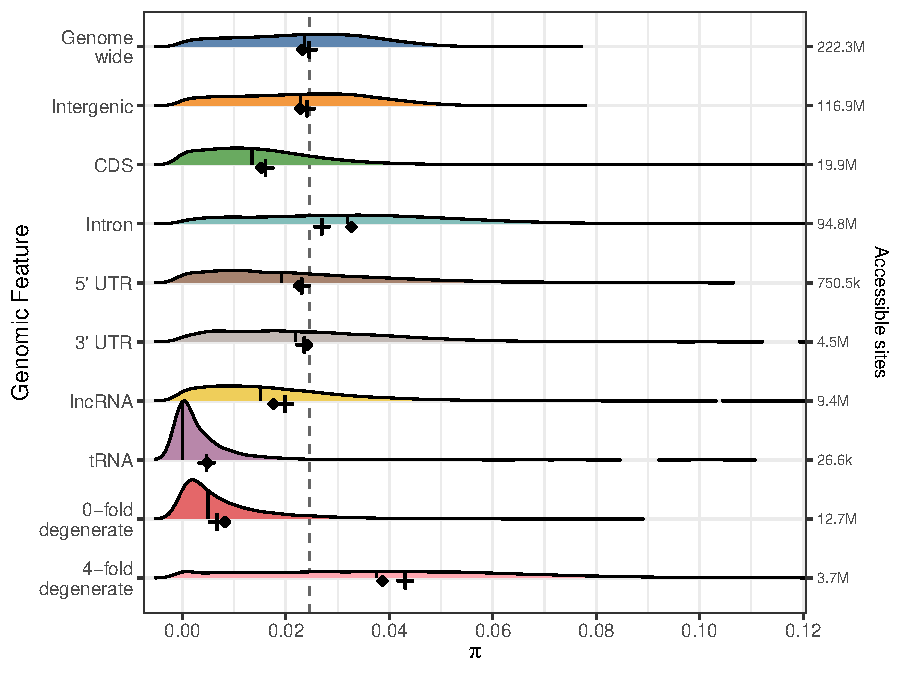
\includegraphics[width=0.6\textwidth]{figures/feature_pi.pdf}
    \caption{\textbf{Nucleotide diversity ($\pi$) across genomic
        features in Oregon \balgla.}
        The density histogram shows the distribution of windowed
        $\pi$ values across different genomic features annotated
        in the \bgla{} assembly. The vertical lines show the
        50\textsuperscript{th} quantile (median) of the distribution,
        while the crosses show the mean value.}
    \label{fig:feature_pi}
\end{figure}

\subsection*{Linkage disequilibrium decays within a few hundred base pairs}\label{sec:results_ld}

\llabel{ld_decay_results}To describe recombination along the genome, we measured how linkage
disequilibrium (LD) decays with the distance between SNPs.
With only six unphased diploid individuals, the usual measures of LD are not reliable.
In 10\,kbp windows, the mean $r^{2}$ between SNPs \citep[$Z_{nS}$;][]{kelly_test_1997},
calculated from genotypes \citep{rogers_linkage_2009}, was close to its sampling floor
for six individuals (median: 0.247), and it decreased as the number of SNPs in the
window increased (Spearman's $\rho$: $-0.52$).
Thus, windows with different SNP densities could not be compared.
We therefore used \sdsq{}, the ratio of the expected $D^{2}$ to the expected
product of allele-frequency variances at the two sites ($\pi_{2}$)
\citep{ohta_linkage_1969}.
We calculated $D^{2}$ and $\pi_{2}$ with the estimators of
\citet{ragsdale_unbiased_2020}, which are unbiased for the size of the sample and
use genotypes, so they do not need phased haplotypes.
Because these estimators are summed over all pairs of SNPs in a distance class,
\sdsq{} does not depend on the number of SNPs, and it can be compared among
regions with different levels of diversity
(see \nameref{sec:methods_ld}).
\vspace{0.1cm}

LD in \bgla{} decays over a short physical distance.
Over the 93 segments of chromosomes 1--15 (see below), \sdsq{} fell to half
of its value for SNPs 10--20\,bp apart at 162\,bp (95\% CI: 142--185\,bp), and to one
quarter at 705\,bp (579--880\,bp; Figure~\ref{fig:sup_ld_decay}A).
A fit of the equilibrium expectation of \citet{ohta_linkage_1971} gave a population
recombination rate ($4N_{e}r$) of 0.14 (0.12--0.17) per bp.
Divided by the median segment $\pi$ (0.024), this value gives $r/\mu \approx 6$.
However, the equilibrium model does not fit the shape of the decay well: the observed
\sdsq{} is 0.7 times the expected value at 14\,bp, and it is 15 times the
expected value at 10\,kbp (Figure~\ref{fig:sup_ld_decay}A).
We therefore use the fitted $4N_{e}r$ as a summary of the rate of decay, not as an
exact estimate of the recombination rate.
\vspace{0.1cm}

The genome contains large regions of reduced diversity (Figure~\ref{fig:genome_pi}D).
To compare them with the rest of the genome, we divided chromosomes 1--15
(excluding chromosome 16 due to its smaller size and uniformly low $\pi$)
into segments of constant mean $\pi$ with a changepoint method
(see \nameref{sec:methods_segments}).
Of the 93 segments, 29 had $\pi$ lower than 0.75 times the genome-wide value
(low-diversity segments; 199\,Mbp, median length 7.1\,Mbp), and 64 did not
(normal-diversity segments; 632\,Mbp, median length 8.9\,Mbp).
The median $\pi$ was 0.0132 in low-diversity segments and 0.0286 in normal-diversity
segments.
LD was higher in the low-diversity segments at all distances
(Figure~\ref{fig:sup_ld_decay}B).
In these segments, \sdsq{} fell to half of its short-distance value at
373\,bp (316--448\,bp), versus 150\,bp (132--174\,bp) in normal-diversity segments, and the
fitted $4N_{e}r$ was 0.036 per bp (0.028--0.051), against 0.15 per bp (0.13--0.18).
We then asked if a difference in $N_{e}$ alone explains this difference in LD decay.
If the two classes differed only in $N_{e}$, the low-diversity curve would equal the
normal-diversity curve with its distances scaled by the ratio of $\pi$ between the
two classes (0.46).
It did not: at the scaled distances, the low-diversity segments had 1.4 to 2.2 times
more LD, and the 95\% confidence intervals did not include 1 at any distance
(Figure~\ref{fig:sup_ld_decay}C).
The ratio of $4N_{e}r$ to $\pi$, which estimates $r/\mu$, gives the same result.
It was 2.7 (2.2--4.3) in the low-diversity segments, against 5.4 (4.6--6.3) in the
normal-diversity segments (ratio 0.51, 0.38--0.83).
Thus, our low-diversity segments have less recombination per mutation, additional LD
caused by linked selection, or both.

\subsection*{Diversity, but not divergence, increases with the population recombination rate}\label{sec:results_pi_rho}

\llabel{pi_rho_results}Linked selection, either background selection or recurrent
selective sweeps, removes more neutral diversity where recombination is low
\citep{kaplan_hitchhiking_1989,begun_levels_1992,charlesworth_effect_1993}.
To test for this pattern, we fitted $4N_{e}r$ in 1\,Mbp windows inside each segment
(827 windows) and compared it with $\pi$ in the same windows.
Because windows in one segment are not independent, all confidence intervals come
from resampling whole segments.
In the normal-diversity segments, $\pi$ increased with $4N_{e}r$ (Spearman's $\rho$:
0.53, 95\% CI: 0.40--0.63; 631 windows).
The correlation was similar when we included the low-diversity segments
(Spearman's $\rho$: 0.48, 0.33--0.60; 827 windows).
Some windows with very low diversity ($\pi < 0.008$) likely contain a large proportion of
genotyping errors, which carry no LD and increase the fitted $4N_{e}r$.
When we removed these 59 windows, the correlation in all segments was 0.57
(0.46--0.66).
The same pattern was present among whole segments (normal-diversity: 0.66, 0.52--0.81;
normal- and low-diversity: 0.59, 0.41--0.73).
Within the low-diversity segments alone, we found no clear relationship
(Spearman's $\rho$: $-0.26$, $-0.49$--0.03; 196 windows), and the negative value came
from the windows with $\pi < 0.008$.
\vspace{0.1cm}

\llabel{div_rho_results}A positive correlation between diversity and recombination
has two possible causes.
Under linked selection, $N_{e}$ is lower where recombination is low, and this reduces
diversity but not divergence between species.
If recombination is mutagenic, the mutation rate is higher where recombination is
high, and this increases both diversity and divergence
\citep{begun_levels_1992}.
To separate these causes, we compared $4N_{e}r$ with divergence between \bgla{} and
\textit{B. crenatus} at 4-fold degenerate sites ($d_{4}$) in the exons of the same
1\,Mbp windows.
In these windows, $\pi$ at 4-fold degenerate sites ($\pi_{4}$) increased with
$4N_{e}r$ (Spearman's $\rho$: 0.39, 0.27--0.50, in 611 normal-diversity windows; 0.43,
0.30--0.54, in all 790 windows).
However, $d_{4}$ did not increase with $4N_{e}r$ (normal-diversity: $-0.05$,
$-0.21$--0.11; all: $-0.08$, $-0.21$--0.07).
The upper limits of these confidence intervals are much lower than the correlation of
$\pi_{4}$ with $4N_{e}r$, so this result is not due to a lack of statistical power.
Also, $d_{4}$ was not correlated with $\pi$ (normal-diversity: 0.09, $-0.05$--0.24;
all: 0.11, $-0.03$--0.25).
The ratio $\pi_{4}/d_{4}$, which removes differences in the mutation rate among
windows, increased with $4N_{e}r$ at least as much as $\pi_{4}$ did (normal-diversity:
0.44, 0.32--0.55; all: 0.47, 0.32--0.58).
Thus, mutagenic recombination does not explain the correlation between diversity
and recombination in \bgla{}.
\vspace{0.1cm}


% Note, update this. The new panel in the main figure covers this so we
% need to make sure they are in sync.
Both $\pi$ and $4N_{e}r$ are proportional to $N_{e}$.
Thus, their correlation is expected when $N_{e}$ varies along the genome, as it does
under linked selection, even if $r$ is constant.
In normal-diversity windows, the slope of $\log(4N_{e}r)$ on $\log(\pi)$ was 1.46
(0.87--2.08), which includes the value of 1 expected if only $N_{e}$ varies.
Together, these results show that the variation in $\pi$ along the genome is a
variation in $N_{e}$, not in the mutation rate, as expected under linked selection.

Both $\pi$ and $4N_{e}r$ are proportional to $N_{e}$.
Thus, their correlation is expected when $N_{e}$ varies along the genome, even if $r$
is constant; in that case, the slope of $\log(4N_{e}r)$ on $\log(\pi)$ is 1.
Among normal-diversity segments, the slope was 2.53 (1.94--3.12;
Figure~\ref{fig:genome_pi}E), and it was 1.92 (1.34--2.45) among normal-diversity
windows. Both exclude 1, so $4N_{e}r/\pi$, which estimates $r/\mu$, increases with $\pi$.
Because $d_{4}$ did not increase with $4N_{e}r$, this is not caused by variation in the
mutation rate, but by a higher recombination rate where diversity is higher.
The relationship remained when we controlled for the number of SNPs and the length of
each segment (partial Spearman's $\rho$: 0.55, 0.35--0.73), and $\sigma_{D}^{2}$ for
SNPs 20--30\,bp apart, which does not depend on the Ohta--Kimura model, decreased with
$\pi$ under the same control ($-0.57$, $-0.74$ to $-0.37$).
Together, these results show that diversity along the \bgla{} genome is lower where
recombination is lower, as expected under linked selection, and that this pattern is
not explained by variation in the mutation rate.


\subsection*{\balgla{} exhibits large effective population sizes}

We estimated the effective population size (\Ne{}) for a central
Oregon \textit{B. glandula} population sample using the whole-genome genotypes.
As a simple estimate of the long-term \Ne{} of this population, we first
calculated \Ne{} using Watterson's estimator of genetic diversity ($\theta_\text{W}$),
observing a mean genome-wide $\theta_\text{W}$ of 0.0617\comment{[Old pixy value; pixy dropped invariant sites with QUAL $<$ 30, so $\pi$ and $\theta_W$ are about 2$\times$ too high. Corrected pooled $\theta_W$ = 0.0294, which gives $N_e \approx 2.5\times10^{6}$ with $\mu = 3\times10^{-9}$. Update.]} (median: 0.0635, standard
deviation: 0.0224; Figure~\ref{fig:sup_theta_ne}). Assuming a per-base,
per-generation mutation rate ($\mu$) of $3\times10^{-9}$ (as estimated by
\cite{nunez_footprints_2020} for the northern acorn barnacle \textit{S. balanoides})
and using the relationship between \Ne{} and $\theta_\text{W}$, this yields a
mean effective size of 5{,}137{,}172 (median: 5{,}289{,}211, standard deviation:
1{,}862{,}683), which is consistent with the expectation of large \Ne{} in this species.
\vspace{0.1cm}

Additionally, we estimated \Ne{} through time using a coalescent-based
approach with \textsc{msmc2} \citep{dutheil_msmc_2020}. This estimate also placed
the historical effective size of the population on the order of $10^{6}$ individuals
(between $10^{6}$ and $10^{7}$ generations ago) (Figure~\ref{fig:sup_mcmc_ne});
however, given our small sample size and the use of only within sample pairwise
comparisons, we were unable to obtain accurate \Ne{} estimates at more recent
($<10^{5}$ generations) timescales using \textsc{msmc2}.
Nevertheless, even these conservative estimates place \bgla{} among the
largest known effective population sizes for any eukaryote, yet orders of
magnitude below the census sizes observed in the field --- a disparity
central to Lewontin's Paradox and one we return to in the Discussion.

\section*{Discussion}\label{sec:discussion}

\subsection*{Genome evolution in large populations}

Evolutionary processes at large demographic scales are expected to leave distinct
signatures in the genome, several of which are observed in our Pacific acorn
barnacle assembly.
For example, large populations are expected to harbor increased levels of segregating
polymorphism, the product of both the reduction in the stochastic loss due to
genetic drift and the increase in the population-scaled mutation rate.
In accordance, we observe a barnacle genome with extreme levels of genetic diversity,
both at the individual and population level (Figure~\ref{fig:sup_kmers};
Table~\ref{tab:sup_popgen_stats}), a substantial proportion of which is located in
coding sequences.
\vspace{0.1cm}

Similarly, large populations are expected to experience an increase in the efficacy of
purifying selection, which is expected to reduce the levels of diversity and increase 
conservation across functional sequences.
We see these patterns reflected in the \bgla{} genome.
Putatively functional sites, particularly coding exons and tRNAs, show both increased
levels of sequence conservation (Figure~\ref{fig:phastcons}) and a reduction in
population-level genetic diversity (Figure~\ref{fig:feature_pi};
Table~\ref{tab:sup_feature_pi}) compared to less constrained features of the genome.
Notably, the rank ordering of the enrichment of conserved elements, with tRNAs and CDSs
as the most enriched, parallels findings in insects \citep{siepel_evolutionarily_2005},
suggesting that the targets of purifying selection are broadly conserved across
arthropods despite the much larger and more repeat-rich genome of \bgla{}.
Increased efficacy of purifying selection is also reflected in the results of the
McDonald-Kreitman test (Figure~\ref{fig:mkTest}), where we observe a relative decrease
in the proportion of non-synonymous polymorphism in a central Oregon \bgla{} population,
suggesting that weakly deleterious variants are more efficiently purged by selection
\citep{li_reverse_2008}.
Positive selection is also expected to increase in efficacy in large populations,
resulting in the fixation of a larger fraction of beneficial non-synonymous mutations.
We observe this pattern as well: in this central Oregon population, the majority
(54 to 61\%, depending on the metric of $\alpha$ used) of non-synonymous substitutions
reached fixation due to positive selection, a proportion higher than that observed in
diverse \textit{Drosophila} populations \citep{haller_asymptoticmk_2017}.
\vspace{0.1cm}

In large enough populations, selection should be efficacious enough that its effects
extend to synonymous sites, where substitutions are normally considered neutral.
This could result in a bias in the usage of synonymous codons, as different codons are
favored over others due to GC biases, mRNA stability, tRNA abundance, and other factors
\citep{galtier_codon_2018,presnyak_codon_2015}.
These effects are observed in the \bgla{} assembly in the form of reduction in the
effective number of codons seen across protein-coding genes.
On average, \bgla{} uses $\approx$ 43 out of 61 available codons, a greater reduction than
that observed in other metazoan genomes (Figure~\ref{fig:codon_enc};
Table~\ref{tab:sup_enc_summary}).
There is moderate evidence that this bias is not the product of compositional neutral
processes (Figure~\ref{fig:sup_enc_gc3s};~Figure~\ref{fig:sup_enc_reg}), suggesting an
increase in the efficacy of natural selection due to the large size of Pacific acorn
barnacle populations.
Moreover, these biases put into question the neutrality of at least some synonymous
substitutions in this system, which could have important ramifications for the study of
molecular evolution; however, the extent of these effects remain presently unknown and
should be the subject of future study.
\vspace{0.1cm}

In contrast, the distribution of transposable and repeat elements in the
\bgla{} assembly was unexpected, as we find a highly repetitive genome
composed of over 60\% repeats (Figure~\ref{fig:genome_pi};
Table~\ref{tab:sup_repeat_summary}).
Previous work has shown that purifying selection plays a key role in the accumulation
and fixation of transposable elements \citep{merel_relaxed_2025,langmuller_genomic_2023,
bourque_ten_2018}, following the expectation that repetitive sequences are, on average,
slightly deleterious.
Given the increased efficacy of selection we observed in the rest of the genome,
our expectation was to find a relatively small proportion of repeats.
However, the high repeat content observed in the genome does not necessarily
reflect the low efficacy of selection in these populations.
Some could be low-frequency, slightly deleterious variants in the process of being purged
from the population.
Other repeats might represent beneficial genetic variation, as transposable elements are
known to play roles in adaptive evolution \citep{schrader_impact_2019}.
For example, repeat elements can act as regulators of gene expression
\citep{trizzino_transposable_2017,rech_population-scale_2022}, and as such may provide
the regulatory plasticity required for survival in rapidly changing
intertidal environments.
Regardless of their role, disentangling the population-wide repeat landscape and its
fitness effects is likely impossible with a single haploid reference assembly.
Thus, this observation drives the need for larger comparative genomic studies across
barnacle populations before we can fully understand the dynamics of genomic repeats
and transposable elements in this and other large populations.

\subsection*{Molecular evolution in large populations: reconciling \dnds{} and the
McDonald-Kreitman test}\label{sec:discussion_dnds_mkt}

One of the more striking patterns in our results is the apparent discordance between
our two measures of selection on protein-coding genes.
The average pairwise \dnds{} between \bgla{} and \textit{B. crenatus} is 0.206,
indicating that the majority of coding sites are under purifying selection.
Yet the McDonald-Kreitman test reveals a seemingly opposite pattern: $\approx61\%$
of non-synonymous substitutions fixed between these species were driven by
positive selection ($\alpha_\text{asym}$ = 0.610).
At first glance, these results appear contradictory: how can coding sequences be
under strong purifying selection while simultaneously showing pervasive adaptive
evolution?
\vspace{0.1cm}

The resolution lies in the fact that \dnds{} and the McDonald-Kreitman test measure
fundamentally different quantities. The \dnds{} ratio averages across all
non-synonymous sites in a gene, the vast majority of which are under functional
constraint, resulting in a ratio well below one. In contrast, the McDonald-Kreitman
test partitions changes into polymorphism and divergence, using synonymous changes
as a neutral baseline to ask whether there is an \textit{excess} of non-synonymous
fixations relative to the neutral expectation. This test is therefore sensitive to
the subset of non-synonymous mutations that escape purifying selection and reach
fixation, even when most non-synonymous sites in a gene are constrained.
Moreover, pairwise \dnds{} is calculated from a single sequence per species and
therefore incorporates segregating polymorphisms into its divergence estimate. In
species with many weakly deleterious non-synonymous variants segregating at
appreciable frequencies, this can inflate the non-synonymous divergence and distort
estimates of selection \citep{li_reverse_2008}. By explicitly separating
polymorphism from fixation, the McDonald-Kreitman test avoids this conflation.
\vspace{0.1cm}

\citet{li_reverse_2008} compared the performance of \dnds{} and the McDonald-Kreitman
test across human, \textit{Drosophila}, and yeast genomes and found that the two
approaches identify distinct but correlated sets of genes as targets of selection.
Notably, the McDonald-Kreitman test was more powerful than \dnds{} only in
\textit{Drosophila}, the species with the highest polymorphism, where it
identified nearly three times as many genes under positive selection. In the
lower-diversity human and yeast datasets, the pattern was reversed. This finding
suggests that the statistical power of the McDonald-Kreitman test is greatest in
high-polymorphism species, making it particularly well suited for systems like
barnacles where segregating variation is abundant.
\vspace{0.1cm}

The pattern we observe in \bgla{} is thus consistent with theoretical expectations
for large populations: strong purifying selection efficiently removes the majority
of deleterious non-synonymous mutations, keeping \dnds{} low, while at the same time
the increased efficacy of positive selection drives a disproportionate fraction of
the remaining non-synonymous substitutions to fixation, producing a high
$\alpha$. This coupling of strong purifying and positive selection is a hallmark
of evolution in large populations and has been observed in \textit{Drosophila}, where
$\alpha_\text{asym}$ is approximately 0.57 \citep{messer_frequent_2013}.
Our estimate of $\alpha_\text{asym}$ of 0.610 in \bgla{} is comparable to
or slightly higher than that in \textit{Drosophila}, consistent with the expectation
that the even larger effective population size in barnacles further increases the
efficacy of both modes of selection.
\vspace{0.1cm}

\subsection*{Barnacles as models for evolution at biological extremes}

Our work shows that a Pacific acorn barnacle population from central Oregon exhibits
genetic diversity of over 5\% (mean genome-wide $\pi$ of 0.0506).\comment{[Old pixy value; pixy dropped invariant sites with QUAL $<$ 30, so $\pi$ and $\theta_W$ are about 2$\times$ too high. Corrected genome-wide $\pi$ = 0.023 (\texttt{pg\_gpu\_stats}). Update.]}
These levels of genetic diversity are higher than those observed for other model
systems known for their relatively large population sizes.
For example, the genome-wide $\pi$ we observe in this population is approximately
seven-fold\comment{[Old pixy value; pixy dropped invariant sites with QUAL $<$ 30, so $\pi$ and $\theta_W$ are about 2$\times$ too high. With the corrected $\pi$ this ratio is about 3-fold. Update.]} higher than that observed in sub-Saharan populations of
\textit{D. melanogaster} (Figure~\ref{fig:sup_pi_comp})
\citep{nunez_footprints_2025,li_comparative_2025,pool_population_2012,
langley_genomic_2012}.
Indeed, even the $\pi$ observed at 0-fold degenerate sites, the least diverse and
among the most constrained sites in the genome, exceeds the genome-wide diversity
observed in these \textit{Drosophila} populations.\comment{[Old pixy value; pixy dropped invariant sites with QUAL $<$ 30, so $\pi$ and $\theta_W$ are about 2$\times$ too high. The corrected 0-fold $\pi$ (0.0067) no longer exceeds the \textit{Drosophila} genome-wide mean (0.0076, Figure~\ref{fig:sup_pi_comp}); remove or reword this sentence. Update.]}
While elevated, this level of diversity is not unique to barnacles.
Similar magnitudes of genome-wide $\pi$ ($\approx10^{-2}$) have been observed
in other metazoan taxa, including corals \citep{meziere_corals_2025}, bivalves
\citep{liu_bivalves_2025}, mosquitoes \citep{kent_aedes_2025,ag1000g}, nematodes
\citep{teterina_nematodes_2023}, and lancelets \citep{braso-vives_highly_2026}.
The bivalve values, however, were computed from variant sites only, after the removal
of sites with a minor allele frequency below 5\% \citep{liu_bivalves_2025}; they are
therefore not per-site diversities and are not directly comparable to ours.
Moreover, as with other marine invertebrates, barnacle life history traits are likely
direct drivers of the elevated polymorphism observed, as factors such as large census
sizes, small propagule size, large brood size, long larval dispersal, and broad geographic
distribution have been positively correlated with high genetic diversity in these
organisms \citep{leffler_revisiting_2012,romiguier_comparative_2014}.
\vspace{0.1cm}

The magnitude of diversity observed in \bgla{} solidly places them among
hyperpolymorphic populations, those exhibiting diversity above 5\%\comment{[Old pixy value; pixy dropped invariant sites with QUAL $<$ 30, so $\pi$ and $\theta_W$ are about 2$\times$ too high. With corrected values, 4-fold $\pi$ = 4.2\% and genome-wide $\pi$ = 2.3\%; reword. Update.]}
\citep{cutter_molecular_2013}. This adds barnacles to a growing list of emerging
hyperpolymorphic model systems, which are key to studying the limits of biological
variation and molecular evolution in natural populations. Moreover, our observations
of extreme genetic diversity also have important implications for the study of species
boundaries. For example, recent work by~\citet{hart_genomic_2025} suggests that levels
of polymorphism above 1\% neutral diversity in eukaryotes likely serve as biological limits
for the definition of species. Barnacles and other hyperpolymorphic populations put these
putative cutoffs into question. We observe levels of genome-wide diversity of over 5\%
in just a very small portion of the biological range of the Pacific acorn barnacle.
Nucleotide diversity is even higher ($\approx8\%$\comment{[Old pixy value; pixy dropped invariant sites with QUAL $<$ 30, so $\pi$ and $\theta_W$ are about 2$\times$ too high. Corrected 4-fold $\pi$ = 4.2\%. Update.]}) at 4-fold degenerate, and putatively
neutral, sites (Figure~\ref{fig:feature_pi}; Table~\ref{tab:sup_feature_pi}).
Given the species' broader geographical and ecological distribution, genetic
diversity is likely to increase when looking across a larger spatial sampling.
This observation reiterates the importance of future studies of genetic diversity
of this species over its whole geographic range, providing some insights on
the mechanisms that maintain population and species boundaries in the presence
of extreme genetic diversity.
\vspace{0.1cm}

Beyond species boundaries, the extreme diversity observed in barnacles also speaks to
a long-standing question in population genetics: the relationship between effective
and census population sizes. From our results on diversity, we
observe that this barnacle population has an effective size of approximately $10^{6}$.\comment{[Old pixy value; pixy dropped invariant sites with QUAL $<$ 30, so $\pi$ and $\theta_W$ are about 2$\times$ too high. Recompute with the corrected $\theta_W$; see also the sea star rate below. Update.]}
However, these populations also show densities of $10^{4}$ individuals per square meter
\citep{menge_recruitment_2000}. Based on this estimate, the census size of the Pacific
acorn barnacle population in central Oregon should be, conservatively, in the billions of
individuals. While the general disparity between the effective and census size estimates
has been highlighted for decades, i.e., Lewontin's Paradox \citep{lewontin_genetic_1974},
the mechanisms underlying the differences have been long debated
\citep{gillespie_role_1999,gillespie_genetic_2000,smith_hitch-hiking_1974,
kimura_neutral_1983} and are still the subjects of study \citep{buffalo_quantifying_2021}.
Our work on the Pacific acorn barnacle provides a unique opportunity to empirically
study this disparity and the biological processes that maintain it.
\vspace{0.1cm}

\subsection*{Barnacles among highly fecund marine invertebrates}

\llabel{marine_sweepstakes}\revpoint{2}{5}With census sizes in the billions and high fecundity,
\bgla{} belongs to the group of marine invertebrates in which the relationship between
census size, effective size, and diversity has been debated for decades.
High fecundity combined with high early mortality can produce a very large variance in
reproductive success, such that a small fraction of adults produces most of the recruits
in each generation.
This sweepstakes reproductive success predicts ratios of effective to census size far
below one and genetic differences among cohorts and sites at small spatial scales
(chaotic genetic patchiness) \citep{hedgecock_does_1994}, and, when the variance is
extreme, genealogies with multiple mergers rather than the Kingman coalescent
\citep{eldon_coalescent_2006}.
Multiple-merger genealogies give an excess of rare variants and can bias estimates of
effective size and demographic history made under the Kingman coalescent.
The negative genome-wide Tajima's $D$ we observe is consistent with population growth,
with linked selection, and with sweepstakes reproduction, and our sample of six
individuals cannot separate these processes.
Our estimates of \Ne{} should therefore be read as the effective size of an equivalent
Kingman population.
\vspace{0.1cm}

\llabel{marine_oysters}Bivalves provide the closest precedent for the patterns in coding sequences that we
report.
In the Pacific oyster, \citet{sauvage_single_2007} found among the highest densities of
synonymous polymorphism then known in animals and studied their relation to codon
usage.
In the European flat oyster, \citet{harrang_high_2013} found a high load of non-neutral
amino-acid polymorphisms: the ratio of non-synonymous to silent diversity was 0.38, at
a synonymous diversity of only 0.006, and the authors related this load to sweepstakes
reproduction.
\bgla{} does not follow this pattern.
Its synonymous diversity is about seven times higher ($\pi_S = 0.042$) and its
$\pi_N/\pi_S$ is about one third as high (0.11).\comment{[Corrected values, from the MK
alignments with all invariant sites counted (revision\_analysis
\texttt{results/comparative}); they replace the pixy values used elsewhere in the
manuscript.]}
This value is inside the range predicted from the synonymous diversity of 86 animal
species, and inside the range of the marine invertebrates among them
\citep{romiguier_comparative_2014,galtier_adaptive_2016}
(Figure~\ref{fig:sup_comparative}).
A high load of amino-acid polymorphism is thus not a general property of highly fecund
marine invertebrates, and in \bgla{} purifying selection on amino-acid variation is as
efficient as its synonymous diversity predicts.
\vspace{0.1cm}

\llabel{marine_sv}Marine invertebrate genomes also carry extensive structural variation.
Gene presence-absence variation is widespread in the Mediterranean mussel
\citep{gerdol_massive_2020}; duplications cover 16.5\% of the eastern oyster genome
across 60 individuals \citep{modak_extensive_2021}; sequences present in only one
haplotype make up about 69\% of each haplotype of a \textit{Crassostrea sikamea}
genome \citep{liu_bivalves_2025}; inversion polymorphisms segregate in \textit{Ciona}
\citep{satou_chromosomal_2021}; and copy number variants make up about one fifth of
sequenced loci in the American lobster, where they, and not SNPs, are associated with
sea temperature \citep{dorant_copy_2020}.
The \bgla{} genome shows signs of the same complexity: a $k$-mer heterozygosity above
3\% (Figure~\ref{fig:sup_kmers}), about 240\,Mbp of haplotig sequence removed during
assembly (Table~\ref{tab:sup_asm_stats}), and a repeat content above 60\%.
Our SNP-based analyses do not capture this variation.
Population samples sequenced with long reads will be necessary to measure the total
genetic variation in \bgla{} and to test whether, as in the lobster, structural
variants carry a large part of its adaptive variation.
\vspace{0.1cm}

\llabel{marine_mutation_rate}Direct estimates of the germline mutation rate now exist for highly
fecund marine invertebrates.
In the crown-of-thorns sea star, $\mu = 9.13 \times 10^{-9}$ per site per generation
(95\% CI $6.5 \times 10^{-9}$ to $1.2 \times 10^{-8}$), from 14 parent-offspring trios
\citep{popovic_high_2024}, three times the rate we used here.
With this rate, our genome-wide diversity gives a long-term \Ne{} of about
$6 \times 10^{5}$ (about $1.2 \times 10^{6}$ from 4-fold degenerate sites), which makes
the gap to census size even larger.\comment{[From corrected $\pi$: genome-wide 0.0231,
4-fold 0.0423.]}
In tunicates, the estimates are indirect, and they suggest a per-generation rate no
higher than in vertebrates \citep{tsagkogeorga_population_2012}.
A high mutation rate thus does not appear to explain the high diversity of these
species, and the gap between effective and census size must come from other processes,
such as linked selection or sweepstakes reproduction.

\section*{Conclusion}

In this work, we take one of the first looks at the genomic signatures of evolution
in large populations using the Pacific acorn barnacle, \balgla{}.
In accordance with population genetics theory, we find evidence for the increased
efficacy of selection in this large barnacle population, manifested as both purifying
selection reducing diversity and maintaining conservation across functional sites, and
pervasive positive selection driving adaptive divergence in protein-coding genes.
Surprisingly, however, we find a highly repetitive genome, in apparent contrast to
the expectation that purifying selection should limit the proliferation of repetitive
sequences.
At the population scale, we observe average genome-wide
nucleotide diversity exceeding 5\%\comment{[Old pixy value; pixy dropped invariant sites with QUAL $<$ 30, so $\pi$ and $\theta_W$ are about 2$\times$ too high. Corrected genome-wide $\pi$ = 0.023 (\texttt{pg\_gpu\_stats}). Update.]}, placing this species among hyperpolymorphic
organisms.
Yet, while this diversity implies large effective population sizes ($\approx10^{6}$\comment{[Old pixy value; pixy dropped invariant sites with QUAL $<$ 30, so $\pi$ and $\theta_W$ are about 2$\times$ too high. Recompute $N_e$ from the corrected $\theta_W$ (0.028). Update.]}
individuals), it still pales in comparison to the estimated census sizes
of this population, underscoring the long-standing disparity between effective
and census population sizes.
Together, these findings establish \bgla{} as a promising emerging model for studying
the mechanisms of evolution at biological extremes.


\input{sections/data_avail.tex}
\input{sections/acknowledgments}
\input{sections/author_contributions}

% Clear a new page for the bibliography
\clearpage

\printbibliography

% Supplements
\clearpage

\fancyhead[L]{\textit{SUPPLEMENTS}}

\input{sections/supplement_methods}

\clearpage

\section*{Supplemental Tables}

% Stats for the different stages of the assembly
\begin{table}[ht]
    \centering
    \suptablecaption{\textbf{Assembly statistics for the \balgla{} genome
        at different stages of the assembly process.}
        Default contigs refers to the sequences assembled by \textsc{hifiasm} with
            default parameters.
        Optimized contigs denotes the sequences generated using \textsc{hifiasm}
            followed by removal of contaminant sequences and purging of haplotigs.
        Hi-C scaffolds refer to the scaffolds generated by \textsc{YaHS}.
        Curated assembly refers to the sequences generated after manual curation of 
            the Hi-C contact map and polishing with \textsc{Inspector}.
        \textsc{BUSCO} results refer to the \texttt{arthropoda\_odb10} dataset.}
    \shadedrows
    \begin{tabular}{lrrrr}
        \toprule
        Assembly Stage &
            \shortstack{Default \\ contigs} &
            \shortstack{Optimized \\ contigs} &
            \shortstack{Hi-C \\ scaffolds} &
            \shortstack{Curated \\ assembly} \\
        \midrule \startshading
        Sequence length (Mbp)          & 1.64        & 1.05        & 1.05       & 1.04 \\
        Fragments (N)                  & \num{4212}  & \num{1342}  & 650        & 592 \\
        Contig N50 (Mbp)               & 0.734       & 1.35        & 1.18       & 1.18 \\
        Scaffold N50 (Mbp)             & \texttt{NA} & \texttt{NA} & 50.96      & 51.41 \\
        \textsc{BUSCO} complete (\%).  & 95.66       & 93.88       & 93.98      & 94.08 \\
        \textsc{BUSCO} single (\%)     & 45.31       & 89.04       & 89.24      & 89.44 \\
        \textsc{BUSCO} duplicates (\%) & 50.35       & 4.84        & 4.74       & 4.64 \\
        \textsc{BUSCO} fragmented (\%) & 0.79        & 1.18        & 0.89       & 0.89 \\
        \textsc{BUSCO} missing (\%)    & 3.55        & 4.94        & 5.13       & 5.03 \\
        \textsc{BUSCO} size (N)        & \num{1013}  & \num{1013}  & \num{1013} & \num{1013} \\
        \bottomrule
    \end{tabular}
    \label{tab:sup_asm_stats}
\end{table}

% Gene-completeness in the annotation
\begin{table}[ht]
    \centering
    \suptablecaption{\textbf{Completeness metrics for the \balgla{} protein-coding
        gene annotation.}
        \textsc{BUSCO} completeness was determined by \textsc{compleasm}
        \texttt{protein}.}
    \shadedrows
    \begin{tabular}{lrr}
        \toprule
        Metric &
            \texttt{arthropoda\_odb10} &
            \texttt{crustacea\_odb12} \\
        \midrule \startshading
        \textsc{BUSCO} complete (\%)   & 93.58      & 84.77 \\
        \textsc{BUSCO} single (\%)     & 79.76      & 72.66 \\
        \textsc{BUSCO} duplicates (\%) & 13.82      & 12.11 \\
        \textsc{BUSCO} fragmented (\%) & 1.78       & 4.10 \\
        \textsc{BUSCO} missing (\%)    & 4.64       & 11.13 \\
        \textsc{BUSCO} size (N)        & \num{1013} & \num{1536} \\
        \bottomrule
    \end{tabular}
    \label{tab:sup_annot_stats}
\end{table}

% Repeat annotation
\begin{table}[htbp]
\centering
\suptablecaption{\textbf{High-level repeat annotation of the \balgla{}
        assembly.}
            Repeats were first identified with the \textsc{EarlGrey} software.
            The classification is the merge of \textsc{EarlGrey}'s homology-based
            assignment, followed by the re-classification of unknown elements by
            \textsc{TEsorter} and \textsc{DeepTE}.
            Coverage is the total number of masked sites per class; ``\% Genome''
            is the coverage divided by assembly size (1{,}043{,}519{,}078\,bp).}
    \label{tab:sup_repeat_summary}
    \shadedrows
    \begin{tabular}{lrrrr}
        \toprule
            Classification &
                Coverage (bp) &
                Count &
                \% Genome &
                \shortstack{Distinct \\ elements} \\
        \midrule \startshading
            DNA                                        & \num{379178613} & \num{895512}  & 36.34 & 35 \\
            LINE                                       & \num{107103442} & \num{223314}  & 10.26 & 20 \\
            LTR                                        & \num{50161694}  & \num{120887}  &  4.81 &  8 \\
            \shortstack[l]{Other (Simple Repeat, \\
                ~~Microsatellite, RNA)}                & \num{37359678}  & \num{74786}   &  3.58 &  3 \\
            Penelope                                   & \num{25833119}  & \num{65921}   &  2.48 &  4 \\
            Rolling Circle                             & \num{22238826}  & \num{42257}   &  2.13 &  1 \\
            Retroposon                                 & \num{2095328}   & \num{5834}    &  0.20 &  2 \\
            SINE                                       & \num{1253619}   & \num{4437}    &  0.12 &  3 \\
            DIRS                                       & \num{1184091}   & \num{1285}    &  0.11 &  2 \\
            Unclassified                               & \num{61450725}  & \num{148647}  &  5.89 &  1 \\
            \midrule
            Total                                      & \num{687859135} & \num{1582880} & 65.92 & 79 \\
    \bottomrule
    \end{tabular}
\end{table}

% Stats about polymorphism in the reference individual and the popgen samples.
\begin{table}[ht]
    \centering
    \suptablecaption{\textbf{Genetic variation in central Oregon \balgla{}.}
        \comment{the ref indidivual stats have to be updated}
        Density of SNPs per accessible kbp is calculated only for windows with more
        than 100 accessible sites ($1000 \times N_\text{window SNPs} / N_\text{window accessible}$).
        Density of SNP in coding sequences was calculated only for exons with more than
        100 accessible sites and adjusting for exon length
        ($1000 \times N_\text{exon SNPs} / N_\text{exon accessible}$).}
    \shadedrows
    \begin{tabular}{lrr}
        \toprule
        Metric &
            Reference Individual &
            Cape Perpetua (N=6) \\
        \midrule \startshading
        Reference sequence length (bp)        & \num{904940360} & \num{904940360} \\
        Accessible sites post-filtering (bp)  & \num{314105136} & \num{231589201} \\
        Total variant sites (N)               & \num{9081889}   & \num{21395217} \\
        Percent variant sites (\%)            & 2.89            & 9.24 \\
        SNPs (N)                              & \num{8725877}   & \num{20495291} \\ % 8.85 of sites
        Indels (N)                            & \num{356012}    & \num{899926} \\
        Multiallelic SNPs (N)                 & \texttt{NA}     & \num{910949} \\ % 4.6% of var sites
        Percent multiallelic SNPs (\%)        & \texttt{NA}     & 4.6 \\
        \midrule
            \rowcolor{white}SNP density \\
        \midrule
        % This is 1000 x N_snps / N_accessible in 1000 bp windows
        Mean SNPs per accessible kbp          & 14.66           & 83.3 \\
        Median SNPs per accessible kbp        & 6               & 80.7 \\
        StDev SNPs per accessible kbp         & 19.86           & 53.9 \\
        \midrule
            \rowcolor{white}Coding variation \\
        \midrule
        % This is 1000 x N_exon_snps x N_exon_accessible across each exon interval
        SNPs in CDS (N)                       & \num{398773}    & \num{1061714} \\
        Percent SNPs in CDS (\%)              & 4.69            & 5.18 \\
        Mean SNPs per accessible CDS kbp      & 4.34            & 51.0 \\
        Median SNPs per accessible CDS kbp    & 1               & 46.5 \\
        StDev SNPs per accessible CDS kbp     & 11.75           & 33.8 \\
        \bottomrule
    \end{tabular}
\label{tab:sup_popgen_stats}
\end{table}

% Stats about the phasCons conserved elements and enrichment of genomic elements.
\begin{sidewaystable}[ht]
    \suptablecaption{\textbf{Enchrichment of annotated features among \textsc{phastCons}
        highly conserved elements.}
        The total feature proportion was determined according to the 841{,}166{,}098\,bp
        corresponding to the 16 chromosome-level scaffolds.
        Proportion of highly-conserved elements (HCE) was calculated based on the
        50{,}849{,}898\,bp-span of all HCEs in the genome.
        The number of chromosomes denotes the number of chromosome-level scaffolds
        containing annotations of the given feature.}
    \centering
    \label{tab:sup_phastcons_enrichment}
    \shadedrows
    \begin{tabular}{lrrrrrrrr}
    \toprule
        Feature &
            \shortstack{Total feature \\ length (bp)} &
            \shortstack{Total feature \\ proportion} &
            \shortstack{HCE feature \\ length (bp)} &
            \shortstack{HCE feature \\ proportion} &
            \shortstack{Mean $\log_2$ \\ enrichment} &
            \shortstack{Median $\log_2$ \\ enrichment} &
            \shortstack{St Dev $\log_2$ \\ enrichment} &
            \shortstack{Number of \\ chromosomes} \\
    \midrule \startshading
        3' UTR     & \num{2358104}   & $2.80\mathrm{e}{-3}$ & \num{152598}   & $3.00\mathrm{e}{-3}$ & $-0.0861$    & 0.0332       & 0.508        & 16 \\
        5' UTR     & \num{530151}    & $6.30\mathrm{e}{-4}$ & \num{27679}    & $5.44\mathrm{e}{-4}$ & $-0.292$     & $-0.332$     & 0.453        & 16 \\
        CDS        & \num{16273411}  & 0.0193               & \num{2225138}  & 0.0438               & 0.752        & 0.984        & 0.926        & 16 \\
        TE         & \num{370573528} & 0.441                & \num{17505920} & 0.344                & $-0.359$     & $-0.305$     & 0.180        & 16 \\
        intergenic & \num{196612776} & 0.234                & \num{10688761} & 0.210                & $-0.167$     & $-0.178$     & 0.167        & 16 \\
        intron     & \num{111562654} & 0.133                & \num{8575960}  & 0.169                & 0.419        & 0.297        & 0.432        & 16 \\
        lncRNA     & \num{2211027}   & $2.63\mathrm{e}{-3}$ & \num{130744}   & $2.57\mathrm{e}{-3}$ & $-0.174$     & $-0.133$     & 0.567        & 16 \\
        multiple   & \num{141022121} & 0.168                & \num{11537936} & 0.227                & 0.418        & 0.438        & 0.167        & 16 \\
        rRNA       & \num{2106}      & $2.50\mathrm{e}{-6}$ & 0.000          & 0.000                & \texttt{NaN} & \texttt{NaN} & \texttt{NaN} & 6 \\
        tRNA       & \num{20220}     & $2.40\mathrm{e}{-5}$ & \num{5162}     & $1.02\mathrm{e}{-4}$ & 2.143        & 2.041        & 0.959        & 16 \\
   \bottomrule
\end{tabular}
\end{sidewaystable}

% Breakdown of per-species codon usage bias
\begin{sidewaystable}[ht]
    \centering
    \small
    \suptablecaption{\textbf{Codon usage biases across metazoan genomes.}
        Table shows the codon usage statistics (effective number of codons; ENC), GC
        proportion, and GC proportion at third codon positions (GC3s) for length-filtered
        (CDS $\geq$ 300\,bp, within 2 standard deviations of the per-species mean length)
        genes in each genome.
        The first four rows (\texttt{BalGla}, \texttt{BalCre}, \texttt{AmpAmp}, and
        \texttt{PolPol}) denote the focal barnacle genomes.}
    \label{tab:sup_enc_summary}
    \shadedrows
    \begin{tabular}{llrrrrrrrrrr}
    \toprule
    & & & \multicolumn{3}{c}{ENC} & \multicolumn{3}{c}{GC} & \multicolumn{3}{c}{GC3s} \\
    \cmidrule(lr){4-6} \cmidrule(lr){7-9} \cmidrule(lr){10-12}
    Genome &
        Species &
        \shortstack{Number \\ of Genes} &
        Mean & Median & StDev &
        Mean & Median & StDev &
        Mean & Median & StDev \\
    \midrule \startshading
    \texttt{BalGla} & \balgla{}                              & \num{16217} & 43.17 & 42.84 & 5.52 & 0.645 & 0.648 & 0.061 & 0.781 & 0.796 & 0.102 \\
    \texttt{BalCre} & \textit{Balanus crenatus}              & \num{7675}  & 42.23 & 41.40 & 4.78 & 0.645 & 0.649 & 0.055 & 0.815 & 0.837 & 0.093 \\
    \texttt{AmpAmp} & \textit{Amphibalanus amphitrite}       & \num{25242} & 44.33 & 43.93 & 5.05 & 0.632 & 0.636 & 0.054 & 0.775 & 0.792 & 0.099 \\
    \texttt{PolPol} & \textit{Pollicipes pollicipes}         & \num{17607} & 42.04 & 41.57 & 4.56 & 0.644 & 0.648 & 0.049 & 0.829 & 0.845 & 0.082 \\
    \texttt{DroMel} & \textit{Drosophila melanogaster}       & \num{12312} & 49.97 & 50.47 & 3.99 & 0.534 & 0.540 & 0.053 & 0.630 & 0.640 & 0.110 \\
    \texttt{AnoGam} & \textit{Anopheles gambiae}             & \num{11804} & 48.43 & 48.92 & 5.09 & 0.556 & 0.566 & 0.062 & 0.667 & 0.688 & 0.136 \\
    \texttt{CaeBre} & \textit{Caenorhabditis brenneri}       & \num{22904} & 50.95 & 51.55 & 3.21 & 0.436 & 0.430 & 0.045 & 0.411 & 0.399 & 0.088 \\
    \texttt{MagGig} & \textit{Magallana gigas}               & \num{24963} & 53.34 & 53.66 & 2.58 & 0.442 & 0.441 & 0.043 & 0.433 & 0.426 & 0.085 \\
    \texttt{StrPur} & \textit{Strongylocentrotus purpuratus} & \num{25759} & 53.92 & 54.39 & 2.68 & 0.481 & 0.480 & 0.035 & 0.489 & 0.486 & 0.079 \\
    \texttt{BraLan} & \textit{Branchiostoma lanceolatum}     & \num{23301} & 51.20 & 51.78 & 3.57 & 0.537 & 0.536 & 0.043 & 0.620 & 0.619 & 0.095 \\
    \texttt{CioInt} & \textit{Ciona intestinalis}            & \num{14370} & 52.49 & 52.75 & 2.66 & 0.424 & 0.422 & 0.037 & 0.369 & 0.367 & 0.069 \\
    \texttt{HomSap} & \textit{Homo sapiens}                  & \num{21573} & 49.39 & 50.57 & 4.51 & 0.538 & 0.541 & 0.087 & 0.593 & 0.603 & 0.163 \\
    \bottomrule
    \end{tabular}
\end{sidewaystable}

% Summary of ENC models
\begin{table}[htbp]
    \centering
    \small
    \suptablecaption{\textbf{Summary of ENC model fits across metazoan genomes.}
        Table shows the fits for the model between the expected and observed effective
        number of codons (ENC) across 12 metazoan genomes.
        ENC deviation values represents the deviation from Wright's curve, as shown in
        Figure~\ref{fig:sup_enc_gc3s}.
        Larger ($\gg0$) values denote a reduction in the observed number of effective
        codons when compared to the GC3s-based expectation, suggesting translational
        selection.
        The linear regression values represent the linear relationship between the
        observed and expected number of effective codons, as seen in Figure~\ref{fig:sup_enc_reg}.
        Deviations in ENC product of translational selection are seen as a reduction in
        both slope and coefficient of determination ($\text{R}^2$).
        }
    \label{tab:sup_enc_models}
    \shadedrows
    \begin{tabular}{llrcccccccc}
    \toprule
    & & & \multicolumn{5}{c}{ENC deviation} & \multicolumn{3}{c}{Linear regression} \\
    \cmidrule(lr){4-8} \cmidrule(lr){9-11}
    Genome &
        Species &
        \shortstack{Number \\ of Genes} &
        Mean & Median & StDev & Min & Max &
        Slope & Intercept & $\text{R}^2$ \\
    \midrule \startshading
    \texttt{BalGla} & \bgla{}                  & \num{16217} & 0.065 & 0.053 & 0.090 & $-0.344$ & 0.571 & 0.580 & 16.18 & 0.492 \\
    \texttt{BalCre} & \textit{B. crenatus}     & \num{7675}  & 0.040 & 0.044 & 0.052 & $-0.235$ & 0.382 & 0.725 & 10.19 & 0.844 \\
    \texttt{AmpAmp} & \textit{A. amphitrite}   & \num{25242} & 0.052 & 0.055 & 0.047 & $-0.225$ & 0.517 & 0.747 & 9.27  & 0.868 \\
    \texttt{PolPol} & \textit{P. pollicipes}   & \num{17607} & 0.025 & 0.032 & 0.054 & $-0.265$ & 0.436 & 0.746 & 9.77  & 0.806 \\
    \texttt{DroMel} & \textit{D. melanogaster} & \num{12312} & 0.092 & 0.092 & 0.039 & $-0.125$ & 0.356 & 0.754 & 8.44  & 0.760 \\
    \texttt{AnoGam} & \textit{A. gambiae}      & \num{11804} & 0.074 & 0.075 & 0.040 & $-0.184$ & 0.480 & 0.779 & 7.58  & 0.871 \\
    \texttt{CaeBre} & \textit{C. brenneri}     & \num{22904} & 0.107 & 0.100 & 0.057 & $-0.079$ & 0.518 & 0.436 & 26.00 & 0.175 \\
    \texttt{MagGig} & \textit{M. gigas}        & \num{24963} & 0.079 & 0.076 & 0.040 & $-0.108$ & 0.567 & 0.560 & 20.89 & 0.330 \\
    \texttt{StrPur} & \textit{S. purpuratus}   & \num{25759} & 0.088 & 0.083 & 0.037 & $-0.287$ & 0.465 & 0.853 & 3.51  & 0.358 \\
    \texttt{BraLan} & \textit{B. lanceolatum}  & \num{23301} & 0.085 & 0.082 & 0.046 & $-0.166$ & 0.487 & 0.642 & 15.17 & 0.624 \\
    \texttt{CioInt} & \textit{C. intestinalis} & \num{14370} & 0.060 & 0.057 & 0.038 & $-0.156$ & 0.428 & 0.591 & 19.45 & 0.588 \\
    \texttt{HomSap} & \textit{H. sapiens}      & \num{21573} & 0.086 & 0.091 & 0.046 & $-0.201$ & 0.486 & 0.693 & 11.83 & 0.818 \\
    \bottomrule
    \end{tabular}
\end{table}


% Breakdown of the per-feature Pi
\begin{sidewaystable}[ht]
    \centering
    \small
    \setlength{\tabcolsep}{4pt}
    \suptablecaption{\textbf{Nucleotide diversity ($\pi$) across different genomic features.}
        For all features, pooled $\pi$ denotes the total sum of pairwise differences over
        the sum pairwise comparisons ($\sum\text{differences}/\sum\text{comparisons}$) for all
        accessible sites.
        Genome-wide and intergenic statistics are calculated over 10\,kbp windows with at
        \num{1000} accessible sites.
        Diversity over smaller genomic intervals (CDS, introns, 5' UTR, 3' UTR, and lncRNA)
        are calculated on windows with at least 50 accessible sites; $20>$ accessible sites
        for tRNAs.
        Diversity at 0-fold and 4-fold degenerate sites are calculated for exons with
        $\geq50$ accessible sites and pooled over the span of the whole gene.}
    \label{tab:sup_feature_pi}
    \shadedrows
    \begin{tabular}{lrrrrrrrrrrrr}
        \toprule
        & \multicolumn{4}{c}{$\pi$} & &
            \multicolumn{3}{c}{Window length (bp)} & &
            \multicolumn{3}{c}{Accessible sites per window} \\
        \cmidrule(lr){2-5} \cmidrule(lr){7-9} \cmidrule(lr){11-13}
        Feature &
            Pooled & Mean & Median & StDev &
            \shortstack{Number \\ of \\ windows} &
            Mean & Median & StDev &
            \shortstack{Number \\ of \\ sites} &
            Mean & Median & StDev \\
        \midrule \startshading
        % Feature                          pooledPi               meanPi                 medianPi               sdPi                   nWinds        meanWinLen       MedWinLen     sdWinLen         nBP               meanWinBP        medWinBP     sdWinBP
        \shortstack[l]{Genome\\wide}       & 0.0245               & 0.0232               & 0.0235               & 0.0127               & \num{63098} & \num{9999.176} & \num{10000} & 65.586         & \num{222343515} & \num{3523.781} & \num{3154} & \num{1862.624} \\
        Intergenic                         & 0.0241               & 0.0228               & 0.0229               & 0.0130               & \num{38889} & \num{9210.389} & \num{10000} & \num{1961.534} & \num{116883842} & \num{3005.576} & \num{2514} & \num{1737.172} \\
        CDS                                & 0.0161               & 0.0152               & 0.0135               & 0.0112               & \num{77517} & 294.236        & 165         & 451.357        & \num{19880799}  & 256.470        & 158        & 376.958 \\
        Intron                             & 0.0270               & 0.0327               & 0.0319               & 0.0191               & \num{86036} & \num{3592.945} & \num{1002}  & \num{8494.484} & \num{94754847}  & \num{1101.340} & 407        & \num{2741.384} \\
        5' UTR                             & 0.0231               & 0.0226               & 0.0192               & 0.0171               & \num{4636}  & 188.612        & 142         & 157.460        & \num{750453}    & 161.875        & 124        & 130.790 \\
        3' UTR                             & 0.0236               & 0.0241               & 0.0219               & 0.0160               & \num{8111}  & 670.819        & 559         & 485.006        & \num{4457431}   & 549.554        & 455        & 405.146 \\
        lncRNA                             & 0.0198               & 0.0176               & 0.0152               & 0.0132               & \num{26739} & 414.910        & 189         & 524.890        & \num{9385177}   & 350.992        & 176        & 441.441 \\
        tRNA                               & $4.70\mathrm{e}{-3}$ & $4.81\mathrm{e}{-3}$ & 0                    & 0.0102               & 435         & 65.607         & 72          & 17.266         & \num{26650}     & 61.264         & 72         & 18.738 \\
        \shortstack[l]{0-fold\\degenerate} & $6.69\mathrm{e}{-3}$ & $8.25\mathrm{e}{-3}$ & $4.98\mathrm{e}{-3}$ & $9.48\mathrm{e}{-3}$ & \num{15647} & \num{1425.765} & \num{1116}  & \num{1345.175} & \num{12688329}  & 810.911        & 623        & 807.874 \\
        \shortstack[l]{4-fold\\degenerate} & 0.0431               & 0.0387               & 0.0375               & 0.0249               & \num{15647} & \num{1425.765} & \num{1116}  & \num{1345.175} & \num{3718088}   & 237.623        & 178        & 233.329 \\
    \bottomrule
    \end{tabular}
\end{sidewaystable}

% Genebank/RefSeq data used
\begin{table}[ht]
    \centering
    \suptablecaption{\textbf{Publicly available NCBI assemblies used for comparative
        analyses.} For the NCBI accessions, \texttt{GCF\_*} denotes RefSeq assemblies and
        annotations. \texttt{GCA\_*} accessions denote GenBank assemblies and (when available)
        annotations.}
    \shadedrows
    \begin{tabular}{lll}
        \toprule
            Genome & Species & NCBI accession \\
        \midrule \startshading
            \texttt{AmpAmp} & \textit{Amphibalanus amphitrite}       & \texttt{GCF\_019059575.1} \\
            \texttt{AmpAmp} & \textit{Amphibalanus amphitrite}       & \texttt{GCA\_037642225.1} \\
            \texttt{AmpImp} & \textit{Amphibalanus improvisus}       & \texttt{GCA\_964274985.1} \\
            \texttt{CapMit} & \textit{Capitulum mitella}             & \texttt{GCA\_030062745.1} \\
            \texttt{PolPol} & \textit{Pollicipes pollicipes}         & \texttt{GCF\_011947565.3} \\
            \texttt{DroMel} & \textit{Drosophila melanogaster}       & \texttt{GCF\_000001215.4} \\
            \texttt{AnoGam} & \textit{Anopheles gambiae}             & \texttt{GCF\_943734735.2} \\
            \texttt{CaeBre} & \textit{Caenorhabditis brenneri}       & \texttt{GCA\_964036135.1} \\
            \texttt{MagGig} & \textit{Magallana gigas}               & \texttt{GCF\_963853765.1} \\
            \texttt{StrPur} & \textit{Strongylocentrotus purpuratus} & \texttt{GCF\_000002235.5} \\
            \texttt{BraLan} & \textit{Branchiostoma lanceolatum}     & \texttt{GCF\_035083965.1} \\
            \texttt{CioInt} & \textit{Ciona intestinalis}            & \texttt{GCF\_018327825.1} \\
            \texttt{HomSap} & \textit{Homo sapiens}                  & \texttt{GCF\_000001405.40} \\
        \bottomrule
    \end{tabular}
    \label{tab:sup_ncbi_genomes}
\end{table}

% SRA data
\begin{table}[ht]
    \centering
    \suptablecaption{\textbf{Publicly available NCBI short-read archive data used
        for comparative analyses.}}
    \shadedrows
    \begin{tabular}{lll}
        \toprule
            SRA & BioProject & Species \\
        \midrule \startshading
            % SRA                  BioProject             Species
            \texttt{SRR8775109}  & \texttt{PRJNA528777} & \textit{Amphibalanus improvisus} \\
            \texttt{SRR8775110}  & \texttt{PRJNA528777} & \textit{Amphibalanus improvisus} \\
            \texttt{SRR8775111}  & \texttt{PRJNA528777} & \textit{Amphibalanus improvisus} \\
            \texttt{SRR8775112}  & \texttt{PRJNA528777} & \textit{Amphibalanus improvisus} \\
            \texttt{SRR8775113}  & \texttt{PRJNA528777} & \textit{Amphibalanus improvisus} \\
            \texttt{SRR8775114}  & \texttt{PRJNA528777} & \textit{Amphibalanus improvisus} \\
            \texttt{SRR8775115}  & \texttt{PRJNA528777} & \textit{Amphibalanus improvisus} \\
            \texttt{SRR8775116}  & \texttt{PRJNA528777} & \textit{Amphibalanus improvisus} \\
            \texttt{SRR8775117}  & \texttt{PRJNA528777} & \textit{Amphibalanus improvisus} \\
            \texttt{SRR8775118}  & \texttt{PRJNA528777} & \textit{Amphibalanus improvisus} \\
            \texttt{SRR8775119}  & \texttt{PRJNA528777} & \textit{Amphibalanus improvisus} \\
            \texttt{SRR8775120}  & \texttt{PRJNA528777} & \textit{Amphibalanus improvisus} \\
            \texttt{SRR8775121}  & \texttt{PRJNA528777} & \textit{Amphibalanus improvisus} \\
            \texttt{SRR8775122}  & \texttt{PRJNA528777} & \textit{Amphibalanus improvisus} \\
            \texttt{SRR8775123}  & \texttt{PRJNA528777} & \textit{Amphibalanus improvisus} \\
            \texttt{SRR8775124}  & \texttt{PRJNA528777} & \textit{Amphibalanus improvisus} \\
            \texttt{SRR8775125}  & \texttt{PRJNA528777} & \textit{Amphibalanus improvisus} \\
            \texttt{SRR8775126}  & \texttt{PRJNA528777} & \textit{Amphibalanus improvisus} \\
            \texttt{SRR8775127}  & \texttt{PRJNA528777} & \textit{Amphibalanus improvisus} \\
            \texttt{SRR8775128}  & \texttt{PRJNA528777} & \textit{Amphibalanus improvisus} \\
            \texttt{SRR8775129}  & \texttt{PRJNA528777} & \textit{Amphibalanus improvisus} \\
            \texttt{SRR8775130}  & \texttt{PRJNA528777} & \textit{Amphibalanus improvisus} \\
            \texttt{SRR8775131}  & \texttt{PRJNA528777} & \textit{Amphibalanus improvisus} \\
            \texttt{SRR8755479}  & \texttt{PRJNA528169} & \textit{Amphibalanus improvisus} \\
            \texttt{SRR18959849} & \texttt{PRJNA816681} & \textit{Capitulum mitella} \\
            \texttt{SRR14354747} & \texttt{PRJNA725059} & \textit{Capitulum mitella} \\
            \texttt{SRR20067441} & \texttt{PRJNA856037} & \textit{Capitulum mitella} \\
            \texttt{SRR20067442} & \texttt{PRJNA856037} & \textit{Capitulum mitella} \\
            \texttt{SRR20067443} & \texttt{PRJNA856037} & \textit{Capitulum mitella} \\
            \texttt{SRR20067446} & \texttt{PRJNA856037} & \textit{Capitulum mitella} \\
            \texttt{SRR20067447} & \texttt{PRJNA856037} & \textit{Capitulum mitella} \\
            \texttt{SRR20067448} & \texttt{PRJNA856037} & \textit{Capitulum mitella} \\
            \texttt{SRR20067449} & \texttt{PRJNA856037} & \textit{Capitulum mitella} \\
            \texttt{SRR20067444} & \texttt{PRJNA856037} & \textit{Capitulum mitella} \\
            \texttt{SRR20067445} & \texttt{PRJNA856037} & \textit{Capitulum mitella} \\
            \texttt{SRR13527601} & \texttt{PRJNA681321} & \textit{Capitulum mitella} \\
            \texttt{SRR13527602} & \texttt{PRJNA681321} & \textit{Capitulum mitella} \\
            \texttt{SRR13527603} & \texttt{PRJNA681321} & \textit{Capitulum mitella} \\
            \texttt{SRR13527604} & \texttt{PRJNA681321} & \textit{Capitulum mitella} \\
        \bottomrule
    \end{tabular}
    \label{tab:sup_sra_data}
\end{table}



\clearpage

\section*{Supplemental Figures}

% k-mer distribution of the raw hi-fi reads
\begin{figure}[ht]
    \centering
    \captionsetup{width=0.95\linewidth}
    \includegraphics[width=0.8\textwidth]{figures/sups_kmers.png}
    \supfigurecaption{\textbf{\textsc{GenomeScope} profile of the raw PacBio HiFi
        data.} Distribution of 21-mers shows an estimated genome size of
        845.01\,Mbp and a heterozygosity of 3.3\% in the \bgla{}
        reference assembly.}
    \label{fig:sup_kmers}
\end{figure}

% Hi-C contact map
\begin{figure}[ht]
    \centering
    \captionsetup{width=0.95\linewidth}
    \includegraphics[width=1.0\textwidth]{figures/sups_hic.pdf}
    \supfigurecaption{\textbf{Hi-C contact map of the \balgla{} assembly.}
        The contact map shows the assembly following manual curation in
        \textsc{Juicebox}. The numbers (1--16) denote the 16 chromosome-level
        scaffolds. The dashed lines show the boundary between these 16
        chromosome-level scaffolds and the unplaced contigs. Note that this
        numbering does not reflect the final ID of the assembled sequences.
        IDs were re-assigned following additional curation and sorting of the
        sequences.}
    \label{fig:sup_hic}
\end{figure}

% dN/dS
\begin{figure}[ht]
    \centering
    \captionsetup{width=0.95\linewidth}
    \includegraphics[width=0.7\textwidth]{figures/dnds.pdf}
    \supfigurecaption{\textbf{Distribution of the pairwise rate of non-synonymous
        to synonymous substitutions (\dnds{}).}
        The distribution is calculated across 9{,}082 single-copy orthologs
        identified between \balgla{} and \textit{Balanus
        crenatus}. The solid gray line marks the boundary between genes under
        positive selection (\dnds{} $>$ 1) and genes under purifying selection
        (\dnds{} $<$ 1). The dashed and dotted lines show the mean (0.206) and
        median (0.158) \dnds{}, both showing that on average \bgla{} coding
        sequences are evolving under a regime of purifying selection.}
    \label{fig:sup_dnds}
\end{figure}

% Direction of selection.
\begin{figure}[ht]
    \centering
    \captionsetup{width=0.95\linewidth}
    \includegraphics[width=0.7\textwidth]{figures/sups_mkt_dos.pdf}
    \supfigurecaption{\textbf{Distribution of per-gene direction of selection values.}
        The distribution shows Direction of Selection (DoS) calculated across 7{,}056
        single-copy orthologs identified between \balgla{} and
        \textit{Balanus crenatus}. The solid black line at zero marks the boundary
        between genes evolving under a regime of positive selection (DoS $>0$) and
        genes exhibiting an excess of slightly deleterious non-synonymous polymorphism
        (DoS $<0$). The light blue dashed line shows the mean DoS (0.103), while
        the dark blue dotted line shows the median DoS (0.109).
        This distribution shows that, on average, coding sequences in \bgla{} appear
        to be evolving under positive selection.}
    \label{fig:sup_dos}
\end{figure}

% Extended GO terms.
\begin{figure}[ht]
    \centering
    \captionsetup{width=0.95\linewidth}
    \includegraphics[width=0.925\textwidth]{figures/sups_go_extended.pdf}
    \supfigurecaption{\textbf{Significant GO term enrichment among the candidates
        under positive selection in the McDonald-Kreitman test.}
        Enrichment for the 367 candidates under selection with annotated GO terms.
        $p_\text{elim}$ denotes the $p$-value calculated from \textsc{topGO}'s
        \texttt{elim} algorithm.
        Top, middle, and bottom panels show the top 15 most enriched terms across
        the three GO categories: biological processes, cellular component, and
        molecular function.
        }
    \label{fig:sup_go}
\end{figure}

% Coding GC, GC3s, and GC4d
\begin{figure}[ht]
    \centering
    \captionsetup{width=0.95\linewidth}
    \includegraphics[width=1.0\textwidth]{figures/sups_coding_gc.pdf}
    \supfigurecaption{\textbf{Distribution of coding GC proportions across metazoan
        genomes.}
        Top, middle, and bottom panels show the GC proportions coding sequence-wide,
        at 3rd codon positions (GC3s), and at 4-fold degerate sites (GC4d),
        respectively.
        Distribution are shown across 12 metazoan genomes, including four barnacles:
        \bgla{} (\texttt{BalGla}), \textit{B. crenatus} (\texttt{BalCre}),
        \textit{A. amphitrite} (\texttt{AmpAmp}), and \textit{P. pollicipes}
        (\texttt{PolPol}).
        See Table~\ref{tab:sup_enc_summary} for additional description of the
        genomes.}
    \label{fig:sup_coding_gc}
\end{figure}

% ENC vs GC3s
\begin{figure}[ht]
    \centering
    \captionsetup{width=0.95\linewidth}
    \includegraphics[width=1.0\textwidth]{figures/sups_enc_gc3s.png}
    \supfigurecaption{\textbf{Relationship between effective codons and GC content.}
        Nc-plots showing the relationship between GC proportion at 3rd codon positions
        (GC3s; X-axis) and the effective number of codons (ENC; Y-axis) for 12
        metazoan genomes.
        At each panel, each point represents a single gene.
        The black curve shows the expected relationship between GC3s and ENC, according
        to Wright's curve: \wrightenc{}, where $s$ denotes GC3s.
        The ``mean dev'' annotation shows the mean deviation in ENC from the theoretical
        expectation.
        Higher values show a larger proportion of genes showing a smaller than expected
        number of effective codons, a putative signature of translational selection.
        See Table~\ref{tab:sup_enc_summary} for additional description of the
        genomes.}
    \label{fig:sup_enc_gc3s}
\end{figure}

% Exp vs Obs ENC
\begin{figure}[ht]
    \centering
    \captionsetup{width=0.95\linewidth}
    \includegraphics[width=1.0\textwidth]{figures/sups_enc_regression.png}
    \supfigurecaption{\textbf{Relationship between the expected and observed number of
        effective codons.}
        Plots show the observed effective number of codons (ENC; Y-axis) as a function
        of the expected ENC (X-axis), as defined by Wright's curve, for 12 metazoan
        genomes.
        At each panel, points represents single genes.
        Dashed line shows the one-to-one relationship, while the solid black line
        shows the linear regression.
        Annotations in the plot show the regression's slope and coefficient of
        determination ($\text{R}^2$).
        Small ($\ll1$) slopes and low $\text{R}^2$ show a reduction in the observed
        number of effective codons when compared to the theoretical expectation,
        a potential signature of translational selection.
        See Table~\ref{tab:sup_enc_summary} for additional description of the
        genomes.}
    \label{fig:sup_enc_reg}
\end{figure}

% Pi vs other species.
\begin{figure}[ht]
    \centering
    \captionsetup{width=0.95\linewidth}
    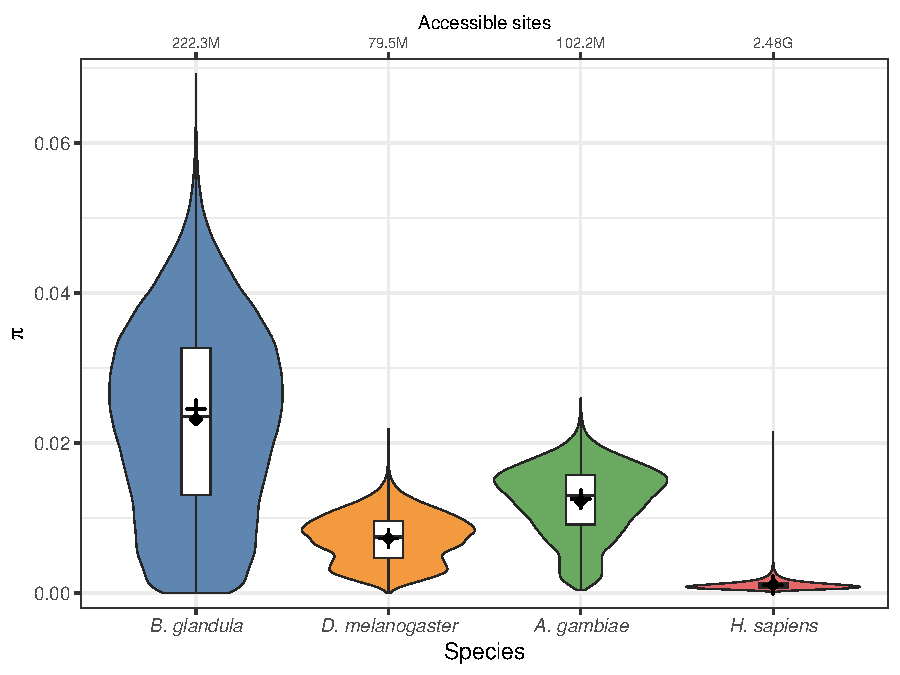
\includegraphics[width=0.9\textwidth]{figures/sups_pi_comparisons.pdf}
    \supfigurecaption{\textbf{Comparing nucleotide diversity ($\pi$) between
        barnacles and biological model systems.}
        Average $\pi$ in 10\,kbp windows between the
        Oregon Pacific acorn barnacle (\balgla{}; \texttt{BalGla}),
        Sub-Saharan populations of the fruit fly (\textit{Drosophila melanogaster};
            \texttt{DroMel}),
        malaria mosquitoes from the Central African Republic (\textit{Anopheles
            gambiae}; \texttt{AnoGam}),
        and human populations of Yoruba ancestry (\textit{Homo sapiens}; \texttt{HomSap}).
        Diamond and crosses denote the mean and pooled (sum of ratios) averages, respectively.
        Consistent with the large \Ne{} expected for \bgla{}, this barnacle population
        exhibits an average (pooled $\pi$) diversity of 0.0242.
        This is $\approx3.4\times$ higher than \textit{Drosophila} (pooled $\pi$ = 0.00728),
        $\approx2\times$ higher than \textit{An. gambiae} (pooled $\pi$ = 0.0125), and
        $\approx23\times$ higher than diverse human cohorts (pooled $\pi$ = 0.00106).}
    \label{fig:sup_pi_comp}
\end{figure}

% Pairwise correlation among different genomic feature and diversity metrics.
\begin{figure}[ht]
    \centering
    \captionsetup{width=0.95\linewidth}
    \includegraphics[width=1.0\textwidth]{figures/sups_pi_pairplot.png}
    \supfigurecaption{\textbf{Pairplot of genomic features and genetic variation
        in Oregon \balgla{}.}
        Diagonal shows the density histogram of the proportion of the genomics
        elements (e.g., CDS, lncRNA, tRNA, repeats, and introns), proportion of
        variant sites, proportion of callable sites post-filtering, and nucleotide
        diversity ($\pi$). All values computed across 10\,kbp windows. Below
        the diagonal, plots show the correlation across all pairwise comparisons.
        Red and blue lines show the linear and Loess regression, respectively.
        Above the diagonal, panels show the Spearman's rank correlation
        coefficient ($\rho$) for the given pairwise comparison.}
    \label{fig:sup_pi_pairplot}
\end{figure}

% Decay of LD with distance
\begin{figure}[ht]
    \centering
    \captionsetup{width=0.95\linewidth}
    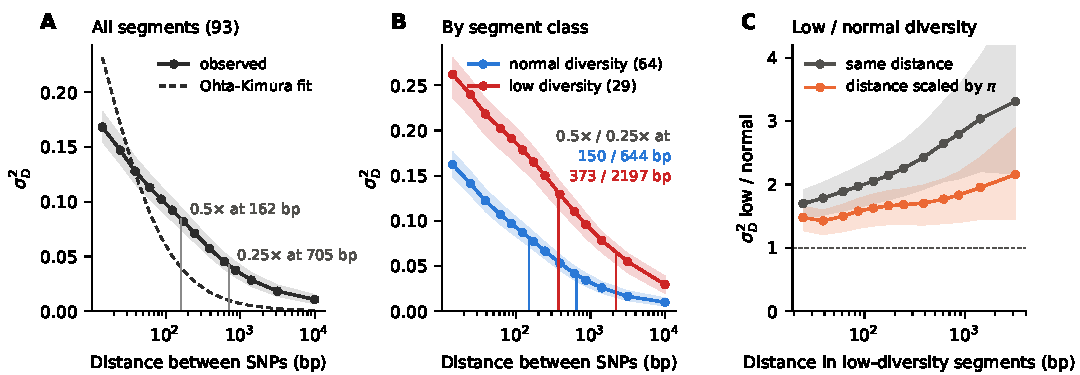
\includegraphics[width=1.0\textwidth]{figures/sups_ld_decay.pdf}
    \supfigurecaption{\textbf{Decay of linkage disequilibrium with distance in Oregon
        \balgla{}.}
        \sdsq{} is the sum of $D^{2}$ divided by the sum of $\pi_{2}$ over all
        pairs of SNPs in a distance class, calculated with the unbiased genotype
        estimators of \citet{ragsdale_unbiased_2020}. Points are at the geometric
        midpoint of each distance class. Shaded bands show 95\% confidence intervals
        from resampling segments within each class.
        \textbf{A.} All 93 segments of chromosomes 1--15. The dashed line shows the
        fitted expectation of \citet{ohta_linkage_1971} ($4N_{e}r$ = 0.14 per bp). Vertical
        lines show the distances at which \sdsq{} falls to one half and to one
        quarter of its value for SNPs 10--20\,bp apart.
        \textbf{B.} Normal-diversity (64) and low-diversity (29) segments. As in panel A,
        vertical lines show the distance at \sdsq{} falls to one half and to one
        quarter for each class.
        \textbf{C.} Ratio of \sdsq{} in low-diversity segments to \sdsq{}
        in normal-diversity segments, at the same distance (grey) and with the normal-diversity
        distances scaled by the ratio of median segment $\pi$ (0.46; orange). A ratio
        above 1 after scaling shows LD that the lower \Ne{} of the low-diversity
        segments does not explain. The first and last distance classes are not shown.}
    \label{fig:sup_ld_decay}
\end{figure}

% Diversity, divergence, and recombination
\begin{figure}[ht]
    \centering
    \captionsetup{width=0.95\linewidth}
    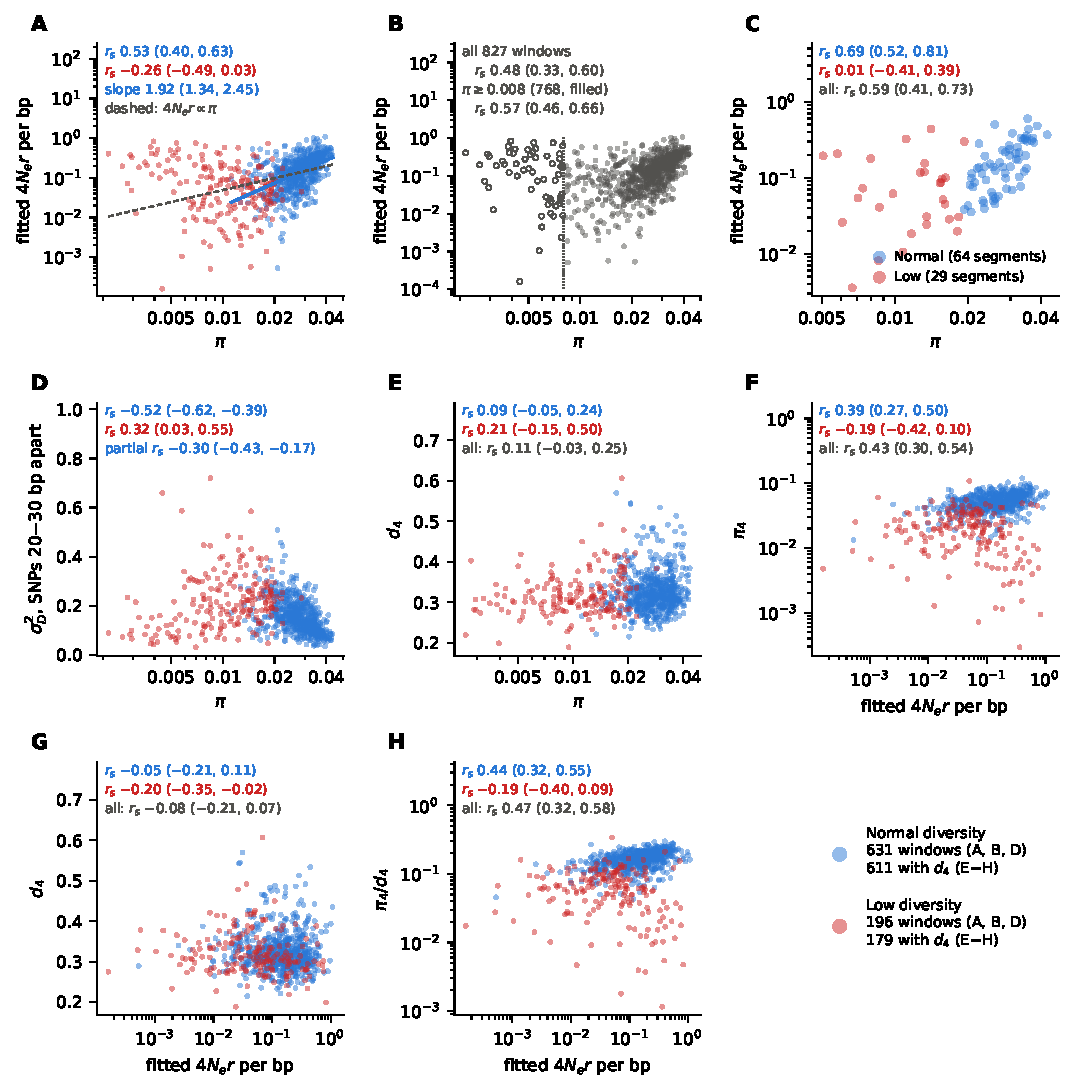
\includegraphics[width=0.95\textwidth]{figures/sups_rho_div.pdf}
    \supfigurecaption{\textbf{Diversity, divergence, and recombination in Oregon
        \balgla{}.}
        Genomic regions of normal (blue) and low (red) diversity are compared for
        metrics of genetic diversity, divergence, and recombination.
        \textbf{A.} Fitted recombination rate $\rho$ ($4N_{e}r$) against $\pi$ in
        normal and low diversity windows 1\,Mbp in length.
        The solid line is the least-squares fit of $\log 4N_{e}r$ on $\log\pi$ in
        normal windows; the dashed line is $4N_{e}r \propto \pi$.
        For all panels, $r_{s}$ denotes the Spearman's correlation coefficient with
        95\% CIs from resampling whole segments.
        \textbf{B.} Fitted $4N_{e}r$ against $\pi$ for all window pooled. The open
        circles show the 59 windows with $\pi < 0.008$.
        \textbf{C.} Fitted $4N_{e}r$ against $\pi$ for normal and low diversity
        segments (defined according to the point change analysis). Complimentary
        plot showing the slopes is shown in Figure~\ref{fig:genome_pi}E.
        \textbf{D.} \sdsq{} for SNPs 20--30\,bp apart against $\pi$ in 1\,Mbp windows.
        The partial $r_s$ count and window length constant.
        \textbf{E.} Divergence at four-fold degenerate sites ($d_4$) against $\pi$
        in 1\,Mbp windows.
        \textbf{F.} Nucleotide diversity at four-fold degenerate sites ($\pi_4$)
        against $4N_{e}r$ in 1\,Mbp windows.
        \textbf{G.} $d_4$ against $4N_{e}r$ in 1\,Mbp windows.
        \textbf{H.} $\pi_4/d_4$ against $N_{e}r$ in 1\,Mbp windows.}
    \label{fig:sup_div_rho}
\end{figure}

% Theta_W Ne
\begin{figure}[ht]
    \centering
    \captionsetup{width=0.95\linewidth}
    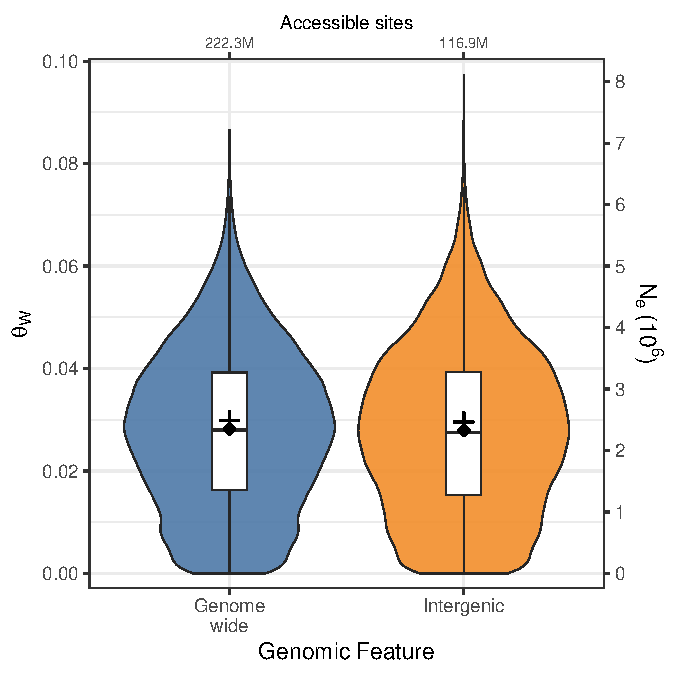
\includegraphics[width=0.8\textwidth]{figures/sups_theta_ne.pdf}
    \supfigurecaption{\textbf{Effective population (\Ne) size estimation
        of \balgla{} based on the Watterson's estimator ($\theta_\text{W}$).}
        Effective size of the population was calculated according to the
        relationship $\theta_\text{W}=4N_{e}\mu$, using a mutation rate per-base,
        per-generation ($\mu$) of $3\times10^{-9}$.
        Diamond and crosses denote the mean and pooled (sum of ratios) averages,
        respectively.
        Estimating pooled $\theta_\text{W}$ across genome-wide and intergenic sites
        in the barnacle genome yield similar long-term \Ne estimates, $2.49\times10^{6}$
        and $2.46\times10^{6}$, respectively.}
    \label{fig:sup_theta_ne}
\end{figure}

% msmc2 Ne
\begin{figure}[ht]
    \centering
    \captionsetup{width=0.95\linewidth}
    \includegraphics[width=0.9\textwidth]{figures/sups_msmc2_ne.pdf}
    \supfigurecaption{\textbf{Coalescent estimation of the effective
    population (\Ne) size estimation of \balgla{}.}
        Estimation of \Ne{} through time was done using the
        \textsc{msmc2} software, using a mutation rate per-base,
        per-generation ($\mu$) of $3\times10^{-9}$, and fixing the
        generation time ($g$) to 1.
        Each line represents the \Ne{} trajectory for each sample.
        Using just six diploid samples, and estimating only between pairs
        of unphased diploid genotypes within samples, we estimate the
        historical effective size of the population in the order of $10^{6}$
        individuals; however, we do not obtain enough resolution to resolve
        \Ne{} at recent ($<10^{5}$) time intervals.}
    \label{fig:sup_mcmc_ne}
\end{figure}

% B. glandula against published comparative data (Romiguier 2014, Galtier 2016)
\begin{figure}[ht]
    \centering
    \captionsetup{width=0.95\linewidth}
    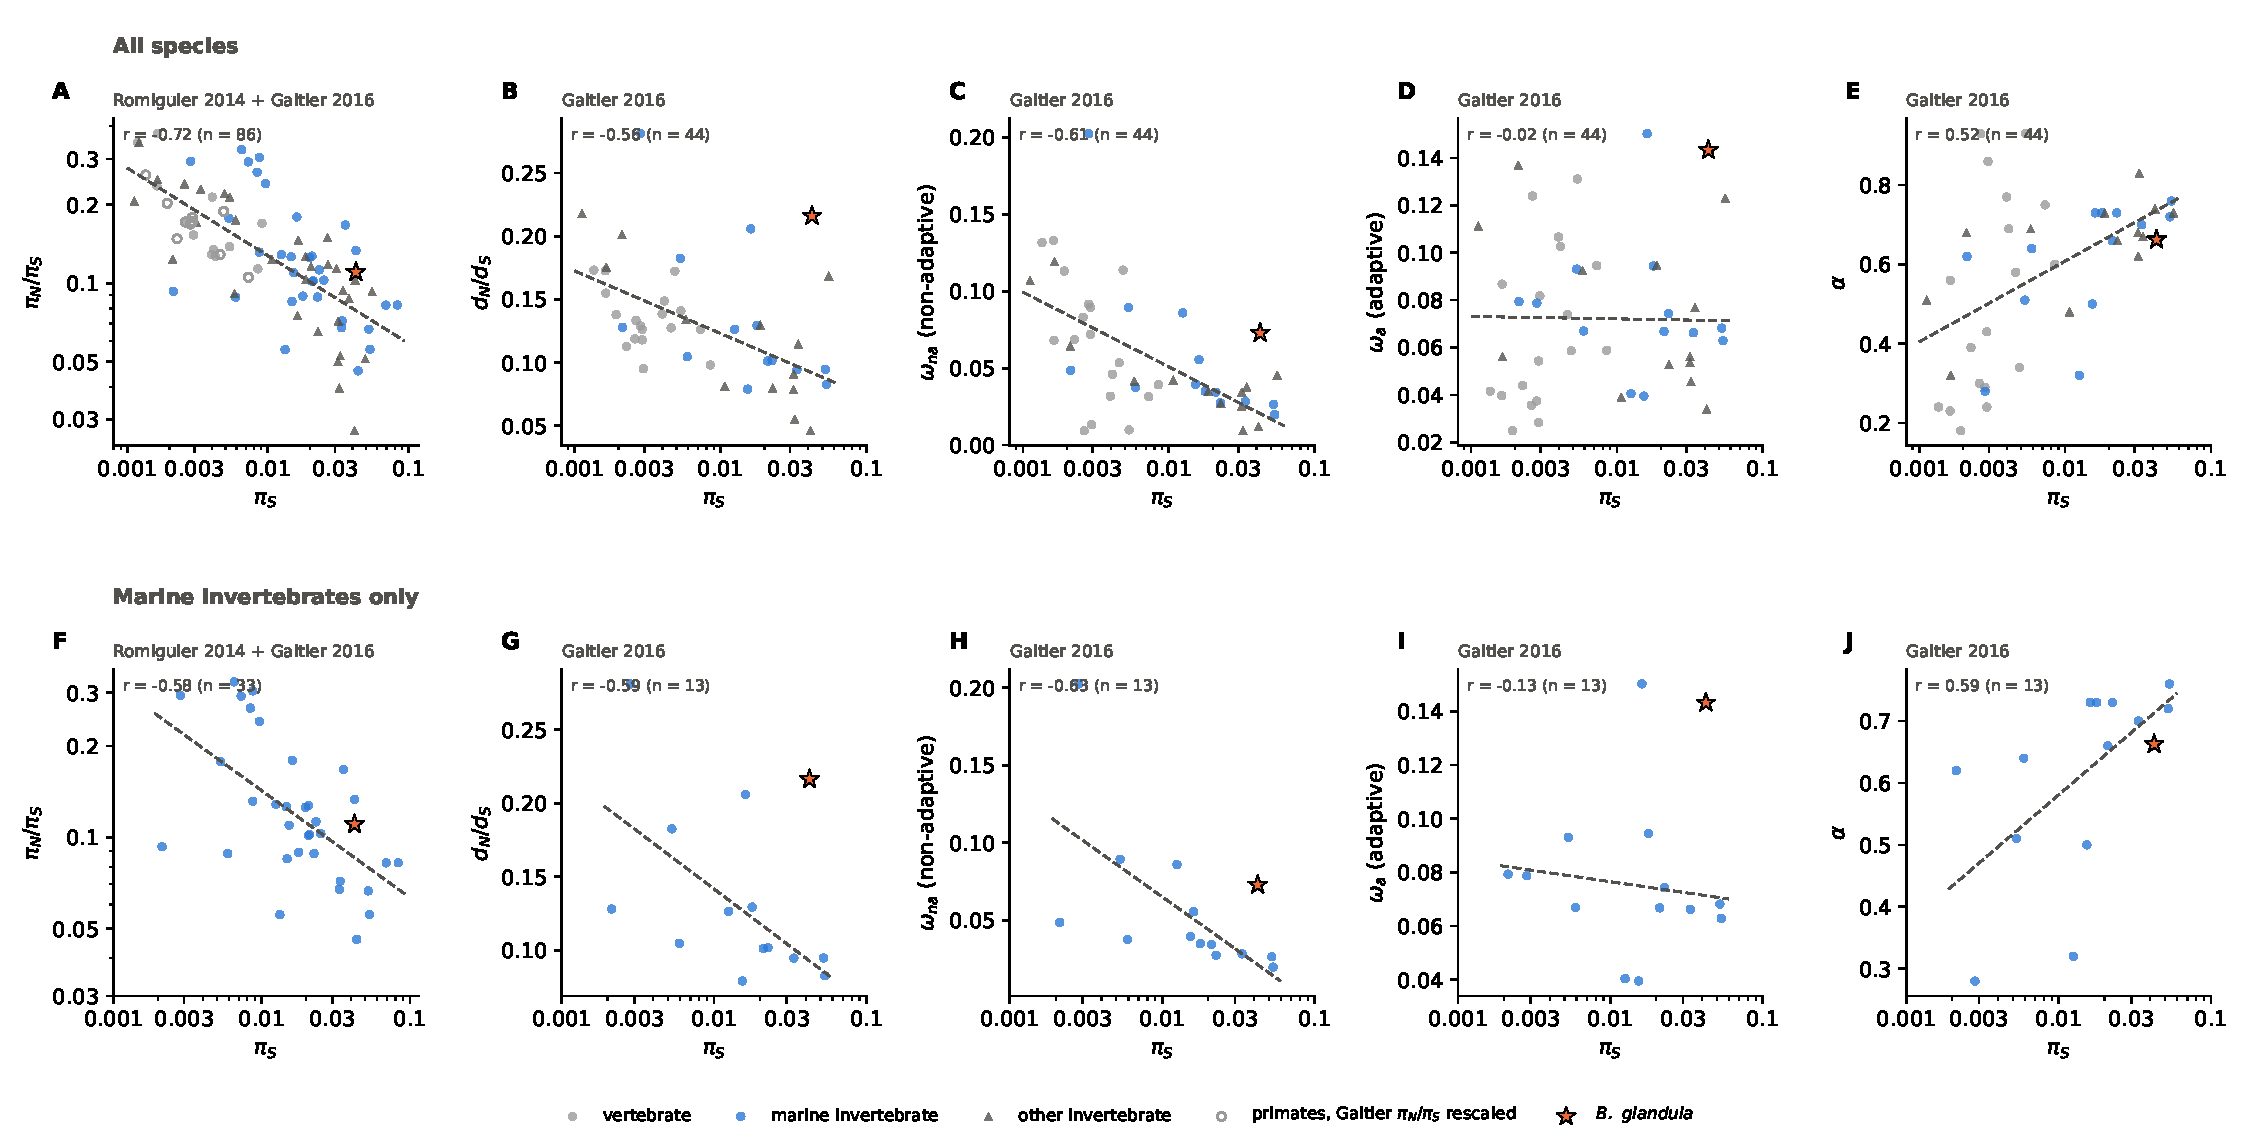
\includegraphics[width=1.0\textwidth]{figures/sups_comparative.pdf}
    \supfigurecaption{\textbf{\bgla{} in the context of published animal data.}
        Synonymous diversity ($\pi_S$) against (A, F) the ratio of non-synonymous to
        synonymous diversity ($\pi_N/\pi_S$), (B, G) \dnds{}, (C, H) the rate of
        non-adaptive amino-acid substitution ($\omega_{na}$), (D, I) the rate of
        adaptive amino-acid substitution ($\omega_{a}$), and (E, J) the proportion of
        adaptive amino-acid substitutions ($\alpha$). Top row (A--E): all species;
        bottom row (F--J): marine invertebrates only. Points are species from
        \citet{romiguier_comparative_2014} and \citet{galtier_adaptive_2016} (86 species
        for $\pi_N/\pi_S$, 44 for the other panels; 33 and 13 marine invertebrates).
        For ten primates present only in \citet{galtier_adaptive_2016}, $\pi_N/\pi_S$ was
        rescaled to the site convention of \citet{romiguier_comparative_2014} (open
        circles). $\omega_{a}$ and $\omega_{na}$ were computed per site as
        $\alpha \cdot$\dnds{} and $(1-\alpha) \cdot$\dnds{}. Dashed lines are
        least-squares fits of each variable on $\log_{10}\pi_S$; $r$ is the Pearson
        correlation. The star shows \bgla{} (all genes; $\pi_S$, $\pi_N/\pi_S$ and \dnds{}
        from the McDonald-Kreitman alignments; $\alpha$, $\omega_{a}$ and $\omega_{na}$
        from a gamma-exponential distribution of fitness effects fitted to the unfolded
        site frequency spectrum, as in \citet{galtier_adaptive_2016}; bars show 95\%
        bootstrap intervals).}
    \label{fig:sup_comparative}
\end{figure}



% Now this version matches the GENETICS submission.
% Start the edits from here.

% === Review Responses (extracted to a separate PDF by the Makefile) ===
% Revision build only. Records the absolute page number where the
% responses begin into review-responses-pagenum.txt so the Makefile can
% split main_revision.pdf into the manuscript and the response document.
\ifdefined\revisionmode
  \clearpage
  \newwrite\pageinfo
  \immediate\openout\pageinfo=review-responses-pagenum.txt
  \immediate\write\pageinfo{\thepage}
  \immediate\closeout\pageinfo
  \setcounter{page}{1}
  \label{review-responses-start}
  \nolinenumbers
  \pagestyle{plain}
  \fancyhead[L]{}
  \fancyhead[R]{}
  \begin{center}
  {\LARGE \textbf{Response to Reviewers}}\\[1em]
  {\large Large population sizes shape genome evolution in barnacles}
  \end{center}
  \vskip 2em
  % Cover letter and point-by-point reviewer responses.
% Reviewer text is verbatim from genetics_review.txt; \reply{...} blocks
% are scaffolded as TODO placeholders to be filled in during the revision.
% Wherever a change is made in the manuscript in response to a point,
% mark the manuscript line with \revpoint{R}{P} and cite it here with
% \revref (inside the matching {point}) or \revreffull{R}{P}.
%
% Reviewer labels used for \revpoint: E (editors), 1, 2.

\begin{minipage}[b]{2.5in}
  Resubmission Cover Letter \\
  {\it GENETICS} \\
  Manuscript GENETICS-2026-309883
\end{minipage}
\hfill
\begin{minipage}[b]{3.0in}
  \raggedleft
  Angel G.\ Rivera-Col\'on (on behalf of all authors) \\
  \today
\end{minipage}

\vskip 2em

\noindent
{\bf Dear Dr.\ Larracuente,}

\vskip 1em

TODO

\vskip 2em

\noindent\hspace{4em}
\begin{minipage}{4.5in}
\noindent
{\bf Sincerely,}

\vskip 2em

{\bf
  Angel G.\ Rivera-Col\'on (on behalf of all authors)
}\\
\end{minipage}

\vskip 4em

\pagebreak

%%%%%%%%%%%%%%%%%%%%%%%%%%%%%%%%%%%%%%%%%%%%%%%%%%%%%%%%%%%%%%%%%%%%%%%%%
% Editors' comments. Set up by hand rather than with \reviewersection so
% the heading doesn't read "Reviewer E"; points are tagged \revpoint{E}{P}.
\renewcommand{\thereviewer}{E}
\setcounter{point}{0}
\section*{Editors:}

\begin{itquote}
Two experts in the field have reviewed your manuscript, and the editors
have read it as well. As you can see below, both reviewers found your
manuscript well written and your system interesting, but they vary in
their view of the impact. Each reviewer has specific concerns that you
can read at the end of this e-mail. Your work clearly presents a valuable
empirical resource, however the current manuscript does not adequately
place the results in the context of other work in the field. While your
manuscript is not currently acceptable for publication in GENETICS, we
would welcome a substantially revised manuscript. Both reviewers and the
editors have comments and concerns to be addressed in a revised
manuscript.

If you do submit a revised manuscript, the revisions will need to clearly
place this work in a broader context. Please carefully consider the
comments from reviewer 2 as your revise. To be further considered by
GENETICS, the revised manuscript should emphasize how this study
contributes to our understanding of how population size interacts with
population genetic mechanisms. The revised manuscript should include
additional analyses and a major revision to the text.
\end{itquote}

\reply{TODO}

% Editor point #1
\begin{point}{} % dN/dS vs MK tension
There is no need to discuss a tension between dn/ds and the MK tests, as
you explain in the discussion that genes can experience both purifying
and positive selection.
\end{point}

\reply{TODO}

% Editor point #2
\begin{point}{} % purifying vs background selection language
Please carefully revise your language about purifying selection and
background selection, as noted by reviewers. Only use background
selection if you are are referring to the effects of purifying selection
on linked variation.
\end{point}

\reply{We agree, and we have corrected this language throughout the manuscript. We
now use ``purifying selection'' only for the direct removal of deleterious alleles at
the selected sites, and ``background selection'' only for the effect of this removal on
linked neutral variation. Two sentences used ``background selection'' for the direct
effect, and both now say ``purifying selection'' \revref, \llname{purifying_results}.
The Introduction now defines the two effects \llname{intro_linked}. In the Results, we
state that the lower diversity of whole features can come from either effect
\llname{feature_pi_linked}, and that the comparison of 0-fold and 4-fold sites in the
same codons isolates the direct effect \llname{pi0_pi4_direct}. New analyses of
linkage disequilibrium and recombination now support our statements about linked
selection; we describe them in our reply to Reviewer 1, point 1.}

% Editor point #3
\begin{point}{} % TE adaptation too speculative; TE age / size distributions
The discuss of TE adaptation is too speculative based on the data that
you present. A deeper analysis of TE age and size distributions may help
you distinguish between some of your alternative hypotheses.
\end{point}

\reply{TODO}

% Editor point #4
\begin{point}{} % focus on 4-fold pi rather than genomic pi
Don't focus so much on genomic pi. Many factors can influence this,
especially the proportion of repetitive and/or non-functional DNA in a
genome. It is much better for comparative work to focus on 4-fold
degenerate pi, as these sites are easily alignable and under weaker
selection in most lineages.
\end{point}

\reply{TODO}

% Editor point #5
\begin{point}{} % repeat-masked reference for SNP calling?
Please clarify if you used a repeat-masked reference for SNP calling, as
this may affect the level of polymorphism in non-coding regions
especially given the high repeat content of your genome.
\end{point}

\reply{TODO}

% Editor point #6
\begin{point}{} % quantitative context: 4-fold pi, Ne, MK
As noted by reviewer 2, it is important that you make an effort to
quantitatively place your findings in the context of the broader
literature addressing the relationship between 4 fold degenerate pi, Ne,
and MK tests.
\end{point}

\reply{TODO}

% Editor point #7
\begin{point}{} % correlation between dN/dS and synonymous pi
It might be interesting to look at the correlation between dN/dS and
synonymous pi. If directional selection dominates, then the correlation
might be negative.
\end{point}

\reply{TODO}

% Editor point #8
\begin{point}{} % line 47: Hill-Robertson effects
Line 47 - better stated as Hill Robertson effects
\end{point}

\reply{TODO}

% Editor point #9
\begin{point}{} % shared ortholog MK results
It may be interesting to look for shared ortholog MK results, if there
are such comparative resources.
\end{point}

\reply{TODO}

% Editor point #10
\begin{point}{} % Fig 5d: low pi regions / centromeres, physical scale
In Fig 5d, regions of low pi are indicative of centromeres exhibiting
reduced crossing-over. What is the physical scale of the phenomenon? It's
hard to tell from the figure. Are there properties of the variation or
divergence indicative of weaker selection in such regions?
\end{point}

\reply{TODO}

% Editor point #11
\begin{point}{} % lines 908-909: source of mutation rate
Lines 908-909, Please clarify where this mutation rate comes from in the
text. It appears to reference an average of 4 arthropod species rather
than one estimated based on S. balanoides data, as described in the Nunez
PNAS paper.
\end{point}

\reply{TODO}

% Editor point #12
\begin{point}{} % B. crenatus window pi from assembly heterozygosity
Regarding the B. crenatus assembly. Could one estimate a window pi from
heterozygosity in the individual used for the assembly and then
investigate whether the orthologous window pi is correlated in the two
barnacle species?
\end{point}

\reply{TODO}

% Editor point #13
\begin{point}{} % line 954: 'moderate evidence' of non-compositional ENC bias
Line 954, Be explicit about the evidence you are alluding to here
regarding the `moderate evidence' of non-compositional bias in the ENC
reduction.
\end{point}

\reply{TODO}


%%%%%%%%%%%%%%%%%%%%%%%%%%%%%%%%%%%%%%%%%%%%%%%%%%%%%%%%%%%%%%%%%%%%%%%%%
\reviewersection{1}

\begin{itquote}
This is a very strong manuscript that tackles important questions in
evolutionary biology. I agree with the authors that species with
exceptionally large Ne offer unique opportunities to investigate the
efficacy of natural selection and other fundamental evolutionary
processes, making barnacles ideal systems to tackle these questions.

The authors provide a chromosome-level genome assembly and pair this
resource with comprehensive molecular evolutionary analyses that paint a
compelling picture of the strong efficacy of selection in the species.
Overall, I am excited about this paper. I only have a few comments for
the authors to consider:
\end{itquote}

\reply{TODO}

% Reviewer 1 point #1
\begin{point}{Purifying vs.\ Background selection}
I found the evidence for efficient purifying selection in B. glandula
convincing. Yet, I got the impression that the terms ``purifying
selection'' and ``background selection'' were being used somewhat
interchangeably. To me, the manuscript makes a very strong case for the
former, whereas the latter feels harder to establish without additional
information on recombination and patterns of linkage. Since the authors
note that characterizing recombination will be focus of future work, I
encourage caution when invoking background selection in the absence of
those data.
\end{point}

\reply{We thank the reviewer for this point. We agree that we used the two terms
interchangeably, and we have corrected this throughout (see our reply to the editor,
point 2). The two sentences that gave background selection as the cause of the low
diversity in coding sequences now say purifying selection \revref,
\llname{purifying_results}. Our evidence for purifying selection is now the comparison
of 0-fold and 4-fold sites in the same codons, which linked selection cannot explain
\llname{pi0_pi4_direct}.

We also followed the reviewer's advice and examined recombination. Our sample of six
unphased individuals is too small for a recombination map, so we measured the decay of
linkage disequilibrium with the unbiased estimators of
\citet{ragsdale_unbiased_2020}. LD falls to half of its short-distance value within
161\,bp \llname{ld_decay_results}. Nucleotide diversity increases with the fitted
population recombination rate (Spearman's $\rho = 0.54$ in normal-diversity windows)
\llname{pi_rho_results}, but divergence from \textit{B. crenatus} does not
\llname{div_rho_results}. Thus, the correlation comes from variation in \Ne{} along the
genome, not from variation in the mutation rate, which is the signature of linked
selection. Background selection and recurrent selective sweeps both produce this
pattern, and our data cannot separate them. Thus, as the reviewer advises, we do not
attribute the pattern to background selection; we use the general term ``linked
selection'' \llname{disc_linked_selection}.}

% Reviewer 1 point #2
\begin{point}{Adaptive TEs}
The possibility that transposable elements contribute to adaptation in
this species is certainly intriguing. However, I would like to see a
somewhat broader discussion of non-adaptive explanations. The manuscript
paints a very consistent picture of highly efficient selection, and given
those patterns, one has to wonder why (or how) is such TE-rich genome
maintained... could there also be a role for unique dynamics of
insertion-deletion balance, or maybe heterogeneity in the recombination
landscape, etc?
\end{point}

\reply{TODO}

% Reviewer 1 point #3
\begin{point}{Codon bias}
I think the ENC/GC composition analyses are very interesting. Given the
high GC-rich nature of the genome, could GC-biased gene conversion (gBGC)
also have contributed to the observed patterns of codon usage??
\end{point}

\reply{TODO}

% Reviewer 1 point #4
\begin{point}{The balancing selection outlier}
One result that caught my attention was the candidate locus exhibiting a
strong excess of polymorphism relative to divergence. I realize this
observation is not a central focus of the manuscript, and I am not
suggesting additional analyses. However, I was curious whether the
authors have any additional thoughts about this locus. The observation
that this homolog has been implicated in osmotic stress responses makes
the result particularly intriguing, and I wonder whether the authors view
this pattern as potentially consistent with ecological processes capable
of maintaining polymorphism (e.g., intertidal zonation like that of Mpi).
I ask this simply out of curiosity.
\end{point}

\reply{TODO}


%%%%%%%%%%%%%%%%%%%%%%%%%%%%%%%%%%%%%%%%%%%%%%%%%%%%%%%%%%%%%%%%%%%%%%%%%
\reviewersection{2}

\begin{itquote}
This manuscript presents a new chromosome-level genome assembly and a
population genomic analysis of the Pacific acorn barnacle Balanus
glandula, a species characterized by very large census population sizes
and exceptionally high genetic diversity. The authors report genome-wide
nucleotide diversity exceeding 5\%, investigate the distribution of
diversity across functional categories, patterns of codon usage,
demographic history, and adaptive protein evolution. They find reduced
diversity in functional elements, as expected under purifying selection,
and infer a high contribution of positive selection to protein
divergence. Overall, the analyses are carefully conducted and the
manuscript is clearly written. B. glandula is certainly an interesting
addition to the relatively small set of species for which such high
levels of nucleotide diversity have been characterized at the
whole-genome level.

I nevertheless have two major concerns, one concerning the scope of the
study and the other its positioning with respect to the existing
literature.
\end{itquote}

\reply{TODO}


% --- Major concerns ---

% Reviewer 2 point #1
\begin{point}{Scope}
Although I found the analyses technically sound, I am not convinced that
the results provide sufficient conceptual advance.

The main novelty is essentially the detailed genomic characterization of
a single, exceptionally polymorphic species. This is valuable, but highly
polymorphic species have already been included in broad comparative
studies of genetic diversity and molecular evolution, including species
with nucleotide diversity in the same general range. The manuscript
itself cites some of this work, including Cutter's work on highly
polymorphic Caenorhabditis, but the comparative context is narrower than
it should be. Other classical examples include Ciona savignyi,
Caenorhabditis remanei and C. brenneri, and Schizophyllum commune. Large
comparative datasets such as Romiguier et al. (2014) and subsequent
studies by Galtier (on Codon Usage Bias, cited in the ms, or on adaptive
protein evolution, not cited in the ms
\url{https://doi.org/10.1371/journal.pgen.1005774}) have also included
highly polymorphic non-model species (with pi$>$5\%) and investigated the
relationships between genetic diversity, effective population size,
efficacy of purifying selection and adaptive protein evolution.

Consequently, most of the major conclusions here are consistent with
expectations and previous empirical work: very high diversity in a
species with a very large population size, stronger signatures of
purifying selection in functional sequences, and efficient adaptive
protein evolution, although Lewontin's paradox remains. I see
considerable value in documenting these patterns in B. glandula,
particularly with a high-quality genome, but less of a general conceptual
advance than suggested by the manuscript.

I therefore think that this is a good population genomic study, but one
whose contribution is primarily the genomic characterization of an
interesting non-model species.
\end{point}

\reply{TODO}

% Reviewer 2 point #2
\begin{point}{The marine population genetics literature is largely overlooked}
Another concern is the literature review and, consequently, the framing
of the study. I was quite surprised by how little the manuscript engages
with the extensive literature on genetic diversity and population
genetics of marine invertebrates.

Marine invertebrates have been central to discussions of extreme genetic
diversity since the allozyme era. High polymorphism in highly fecund
marine organisms, its relationship with census and effective population
size, and the unusual demographic processes affecting such species have
been studied for decades. In this context, I find it particularly
surprising that the work of Hedgecock and others is not discussed. The
concepts of sweepstakes reproductive success, very large variance in
reproductive success, low Ne/N ratios and, more recently, multiple-merger
coalescents and chaotic genetic patchiness are directly relevant to the
biological interpretation of the patterns reported here.

This omission matters because several observations presented as
characteristic consequences of the exceptional population size of B.
glandula have precedents in marine population genetics. For example, high
nucleotide polymorphism and its consequences for protein variation have
been investigated in marine bivalves for many years. Sauvage et al.
(2007) explicitly studied both nucleotide polymorphism and codon usage in
the Pacific oyster, reporting levels of diversity among the highest known
in animals at the time. Harrang et al. (2013) investigated the unusually
high load of non-neutral amino-acid polymorphisms in the European flat
oyster and explicitly discussed its relationship with high fecundity and
sweepstakes reproduction. More generally, marine genomes are now known to
contain extensive structural variation. Massive gene presence-absence
variation has been described in mussels (e.g. Gerdol et al. 2020), and
abundant CNVs and other structural variants have been documented in
oysters (Modak et al. 2021, Lui et al. 2025) and other marine
invertebrates (e.g. tunicates: Satou et al. 2021, lobster: Dorant et al.
2020). Thus, the genomic complexity observed here should also be
discussed in the context of this literature rather than primarily in
comparison with classical model organisms.

Similarly, mutation rate is no longer entirely unexplored in highly
fecund marine invertebrates. Direct germline mutation-rate estimates are
available, for example in sea stars (Popovic et al. 2024), and relevant
estimates also exist in tunicates. These studies are particularly
relevant to the discussion of Lewontin's paradox because they explicitly
address the respective contributions of mutation rate, census population
size and demographic history to high genetic diversity.

I am not suggesting that all these earlier studies addressed exactly the
same questions or had access to chromosome-level whole-genome data.
Clearly they did not. Rather, my concern is that the manuscript currently
creates the impression that highly polymorphic species, and particularly
highly fecund marine invertebrates, represent a largely unexplored
empirical domain. This is not the case. A more thorough treatment of this
literature would both provide a fairer historical perspective and make it
clearer what the present study genuinely adds.
\end{point}

\reply{We thank the reviewer for this point and agree that the manuscript did not
engage with the marine invertebrate literature. We have made four changes.
(1) The Introduction now places \bgla{} in this literature and in the comparative
studies that include hyperdiverse species, and no longer presents large populations as
an unexplored domain \revref.
(2) A new Discussion subsection, ``Barnacles among highly fecund marine
invertebrates'', discusses sweepstakes reproductive success, low ratios of effective to
census size, chaotic genetic patchiness and multiple-merger coalescents
\citep{hedgecock_does_1994,eldon_coalescent_2006}, and what they mean for our
estimates of \Ne{} \llname{marine_sweepstakes}.
(3) The same subsection compares our coding-sequence results with the oyster studies
the reviewer cites \llname{marine_oysters}. Unlike the flat oyster
\citep{harrang_high_2013}, \bgla{} does not carry a high load of amino-acid
polymorphism: its $\pi_N/\pi_S$ (0.11) is inside the range predicted from its $\pi_S$
across 86 animal species and across the marine invertebrates among them (new
Figure~\ref{fig:sup_comparative}). It also discusses the structural variation
documented in mussels, oysters, tunicates and lobster
\citep{gerdol_massive_2020,modak_extensive_2021,liu_bivalves_2025,
satou_chromosomal_2021,dorant_copy_2020} in relation to the complexity of the \bgla{}
genome \llname{marine_sv}.
(4) The subsection ends with the direct germline mutation rate of the crown-of-thorns
sea star \citep{popovic_high_2024}, which gives a long-term \Ne{} of about
$6\times10^{5}$ to $1.2\times10^{6}$ for \bgla{}, and with the indirect estimates
available for tunicates \citep{tsagkogeorga_population_2012}
\llname{marine_mutation_rate}.}


% --- Additional comments ---

% Reviewer 2 point #3
\begin{point}{} % codon usage: preferred vs unpreferred codons (Fop), gBGC
I am not fully convinced by the codon-usage analysis. ENC is useful as a
general measure of codon bias, but it does not directly identify which
synonymous codons are selectively preferred. In the context of this
manuscript, an analysis based on preferred versus unpreferred codons, for
example using Fop or a related measure after identifying preferred
codons, would be considerably more informative. This is particularly
important because GC3 correction alone does not fully resolve the
distinction between selection on codon usage and GC-biased gene
conversion or other GC-associated processes. Knowing whether preferred
codons are GC- or AT-ending would help discriminate among these
explanations. The literature on codon usage in highly polymorphic
species, including comparative studies by Galtier and colleagues and the
earlier work in Pacific oyster by Sauvage et al. (2007), would provide
useful context here.
\end{point}

\reply{TODO}

% Reviewer 2 point #4
\begin{point}{} % interpreting high alpha; Galtier 2016
Relatedly, I would be cautious about interpreting high alpha from
McDonald-Kreitman analyses too directly as evidence that the
exceptionally large population size of B. glandula produces unusually
strong adaptive evolution. Comparative analyses have already shown that
the relationship between effective population size and alpha is not
straightforward. In particular, Galtier (2016) found that much of the
relationship between diversity and alpha across animals could be
explained by more efficient purifying selection and a reduced
contribution of slightly deleterious substitutions, rather than by a
higher rate of adaptive substitution per se. This distinction seems
particularly relevant here.
\end{point}

\reply{TODO}

% Reviewer 2 point #5
\begin{point}{} % sweepstakes reproduction / multiple-merger coalescents
The demographic interpretation could also engage more explicitly with
reproductive biology. For a highly fecund broadcast-spawning marine
species, a Wright-Fisher model based on conventional Ne should at least
be discussed alongside sweepstakes reproduction and multiple-merger
genealogies. These processes can substantially alter the relationship
between nucleotide diversity, census size and the demographic parameters
inferred under a standard Kingman coalescent.
\end{point}

\reply{TODO}

% Reviewer 2 point #6
\begin{point}{} % connect to existing B. glandula popgen / latitudinal cline
Finally, given that B. glandula itself has a substantial population
genetic and phylogeographic literature, including work on its strong
latitudinal genetic cline, I think the manuscript could do more to
connect the new genome-wide results to what is already known about
population structure and demographic history in this particular species.
\end{point}

\reply{TODO}

% Reviewer 2 point #7
\begin{point}{Overall assessment}
This is a carefully conducted study based on a valuable new genomic
resource, and I have no major concerns about the overall quality of the
analyses. My reservations concern primarily the level of novelty claimed
and the incomplete treatment of previous work. The study provides an
interesting whole-genome characterization of an extremely polymorphic
marine species, but many of its main biological conclusions have
precedents in comparative population genomics and, especially, in the
long-standing literature on highly fecund marine invertebrates. A
substantial revision of the introduction and discussion would therefore
be necessary to place the results in their appropriate context and to
more clearly identify what is genuinely new.
\end{point}

\reply{TODO}

\fi

\end{document}
"
% which turns on line numbers and appends the point-by-point response
% document (genetics_rev1/review-responses.tex) after the supplement.
\ifdefined\revisionmode
  % Macros for reviewer responses and back-links from the response document
% to manuscript line numbers. Pattern adapted from the mkado / popgensbi
% manuscripts.
%
% Loaded only in revision mode (see the \revisionmode block in main.tex).
% Expects the lineno package to be loaded by the calling document and
% \linenumbers to be active in the manuscript body.

% Reviewer / point counters
\newcommand{\thereviewer}{}
\newcounter{point}
\setcounter{point}{0}

% Start a new reviewer block. Argument is the reviewer label
% (e.g. \reviewersection{1} or \reviewersection{AE}).
\newcommand{\reviewersection}[1]{%
  \renewcommand{\thereviewer}{#1}%
  \setcounter{point}{0}%
  \section*{Reviewer \thereviewer:}%
}

% A single review point. Argument is an optional name (often empty).
% Pattern from
% http://tex.stackexchange.com/questions/2317/latex-style-or-macro-for-detailed-response-to-referee-report
\newenvironment{point}[1]
  {\color{gray}\refstepcounter{point}\bigskip\hrule\medskip\noindent
   \slshape{\fontseries{b}\selectfont (\thereviewer.\thepoint) #1}}
  {}

\newcommand{\reply}{\normalfont\medskip\noindent\textbf{Reply}:\ }

% \revpoint{R}{P} marks a manuscript line that addresses reviewer R, point P.
% Use this in the manuscript wherever you make a change in response to a
% reviewer point so the response document can back-link to it.
\newcommand{\revpoint}[2]{\hypertarget{llineno:rev#1:#2}{\linelabel{rr:rev#1:#2}}}

% \revreffull{R}{P} renders a (page, line) reference to such a target.
\newcommand{\revreffull}[2]{{(p.\ \hyperlink{llineno:rev#1:#2}{\pageref{rr:rev#1:#2}, l.\ \lineref{rr:rev#1:#2}})}}

% \revref expands to the page/line reference for the current reviewer/point
% inside a {point} environment.
\newcommand{\revref}{\revreffull{\thereviewer}{\thepoint}\xspace}

% Named back-links: place \llabel{name} in the manuscript, refer to it
% from anywhere with \llname{name}.
\newcommand{\llabel}[1]{\hypertarget{ll:#1}{\linelabel{#1}}}
\newcommand{\llname}[1]{{(p.\ \hyperlink{ll:#1}{\pageref{#1}, l.\ \lineref{#1}})}}

% Italics-quoted block (used to set off the verbatim reviewer text).
\newenvironment{itquote}
  {\begin{quote}\color{gray}\itshape}
  {\end{quote}}

% Convenience macros
\newcommand{\rollover}{\reply{The reviewer makes an excellent point that we have missed out entirely. We have made all the changes suggested, down to the minutiae \revref.}}
\newcommand{\playdead}{\reply{The reviewer makes an excellent point. We have made an utterly trivial change \revref{}that we think deals entirely with the concern raised.}}

% lineno + amsmath fix: lineno doesn't number lines inside align/equation
% environments by default. Patch from
% http://tex.stackexchange.com/questions/43648
\ifcsname patchAmsMathEnvironmentForLineno\endcsname
\else
\newcommand*\patchAmsMathEnvironmentForLineno[1]{%
  \expandafter\let\csname old#1\expandafter\endcsname\csname #1\endcsname
  \expandafter\let\csname oldend#1\expandafter\endcsname\csname end#1\endcsname
  \renewenvironment{#1}%
    {\linenomath\csname old#1\endcsname}%
    {\csname oldend#1\endcsname\endlinenomath}}
\newcommand*\patchBothAmsMathEnvironmentsForLineno[1]{%
  \patchAmsMathEnvironmentForLineno{#1}%
  \patchAmsMathEnvironmentForLineno{#1*}}
\AtBeginDocument{%
  \patchBothAmsMathEnvironmentsForLineno{equation}%
  \patchBothAmsMathEnvironmentsForLineno{align}%
  \patchBothAmsMathEnvironmentsForLineno{flalign}%
  \patchBothAmsMathEnvironmentsForLineno{alignat}%
  \patchBothAmsMathEnvironmentsForLineno{gather}%
  \patchBothAmsMathEnvironmentsForLineno{multline}%
}
\fi

\else
  \providecommand{\revpoint}[2]{}%
  \providecommand{\revref}{}%
  \providecommand{\revreffull}[2]{}%
  \providecommand{\llabel}[1]{}%
  \providecommand{\llname}[1]{}%
\fi
% ---------------------------------------------------------------------
